% From Scratch to Python: a Google Colab workbook for a 9-year-old (expanded edition).
% Compile with:  tectonic scratch-to-python-workbook.tex
% The shared look lives in preamble.tex; each part lives in chapters/.
% The previous single-file edition is kept as scratch-to-python-workbook-v2-backup.tex.
\documentclass[12pt,a4paper]{article}
% Shared preamble for the workbook and the chapter test harness.
\usepackage[a4paper,margin=2cm,top=2cm,bottom=2.2cm]{geometry}
\usepackage{fontspec}
\usepackage{FiraSans}
\setmonofont{FiraMono}[Extension=.otf, UprightFont=*-Regular, BoldFont=*-Bold, Ligatures=NoCommon]
\renewcommand{\familydefault}{\sfdefault}
\usepackage{xcolor}
\usepackage{amssymb}
\usepackage{array,longtable,booktabs}
\usepackage{enumitem}
\usepackage{needspace}
\newcolumntype{P}[1]{>{\raggedright\arraybackslash}p{#1}}
\usepackage{listings}
\usepackage[most]{tcolorbox}
\usepackage{tikz}
\usetikzlibrary{arrows.meta,calc,shapes.geometric}
\usepackage{scratch3}
\usepackage{fancyhdr}
\usepackage[hidelinks]{hyperref}

\linespread{1.22}
\setlength{\emergencystretch}{3em}
\setlength{\parindent}{0pt}
\setlength{\parskip}{7pt}
\setlist{itemsep=3pt,topsep=4pt}
\setscratch{scale=1, else word=else}

% ---------- Scratch colours ----------
\definecolor{motion}{HTML}{4C97FF}
\definecolor{looks}{HTML}{9966FF}
\definecolor{sound}{HTML}{CF63CF}
\definecolor{events}{HTML}{FFBF00}
\definecolor{control}{HTML}{FFAB19}
\definecolor{sensing}{HTML}{5CB1D6}
\definecolor{operators}{HTML}{59C059}
\definecolor{variables}{HTML}{FF8C1A}
\definecolor{lists}{HTML}{FF661A}
\definecolor{myblocks}{HTML}{FF6680}
\definecolor{pen}{HTML}{0FBD8C}
\definecolor{ink}{HTML}{1B2550}
\definecolor{muted}{HTML}{56618A}
\definecolor{codebg}{HTML}{F3F6FD}
\definecolor{codeframe}{HTML}{9AA8D4}
\definecolor{kw}{HTML}{1D4FC4}
\definecolor{str}{HTML}{1B7F3B}
\definecolor{com}{HTML}{7A84A8}
\definecolor{warnbg}{HTML}{FFF3DB}
\definecolor{warnframe}{HTML}{E89A12}
\definecolor{chalbg}{HTML}{E6F7EC}
\definecolor{chalframe}{HTML}{2E9C57}
\definecolor{thinkbg}{HTML}{E8F0FF}
\definecolor{thinkframe}{HTML}{4C7FE0}
\definecolor{errbg}{HTML}{FFECEC}
\definecolor{errframe}{HTML}{D23B3B}\colorlet{errhead}{errframe!35}
\color{ink}

% ---------- Python code ----------
\lstdefinestyle{py}{
  language=Python, basicstyle=\ttfamily\normalsize, keepspaces=true, columns=fixed,
  upquote=true, showstringspaces=false, keywordstyle=\color{kw}\bfseries,
  stringstyle=\color{str}, commentstyle=\color{com}\itshape,
  morekeywords={True,False,None}, deletekeywords={print,input,range,int,str,len,abs,round},
  numbers=left, numberstyle=\scriptsize\color{muted}, numbersep=9pt, xleftmargin=0pt,
  tabsize=4, breaklines=true
}
\lstdefinestyle{inl}{style=py, numbers=none, basicstyle=\ttfamily}
\newcommand{\py}{\lstinline[style=inl]}
\DeclareTextCommand{\textvisiblespace}{TU}{\makebox[0.6em][c]{\color{muted}\rule{0.5pt}{0.35ex}\rule{0.45em}{0.5pt}\rule{0.5pt}{0.35ex}}}
\makeatletter\def\lst@visiblespace{\textvisiblespace}\makeatother

\newtcblisting{typethis}[1][Type this into a code cell]{
  listing only, enhanced, colback=codebg, colframe=codeframe, boxrule=0.8pt, arc=6pt,
  left=22pt, right=8pt, top=4pt, bottom=4pt,
  title={\textbf{#1}}, coltitle=white, colbacktitle=ink, fonttitle=\small,
  listing options={style=py}}
\newtcblisting{code}{
  listing only, enhanced, colback=codebg, colframe=codeframe, boxrule=0.6pt, arc=5pt,
  left=22pt, right=6pt, top=2pt, bottom=2pt, listing options={style=py}}
\newtcblisting{codenonum}{
  listing only, enhanced, colback=codebg, colframe=codeframe, boxrule=0.6pt, arc=5pt,
  left=8pt, right=6pt, top=2pt, bottom=2pt, listing options={style=py,numbers=none}}
\newtcblisting{spaces}{
  listing only, enhanced, colback=codebg, colframe=codeframe, boxrule=0.6pt, arc=5pt,
  left=22pt, right=6pt, top=2pt, bottom=2pt, listing options={style=py,showspaces=true}}
\newtcolorbox{outputbox}[1][You should see]{
  enhanced, colback=white, colframe=ink!40, boxrule=0.6pt, arc=5pt, left=8pt,
  title={\textbf{#1}}, coltitle=ink, colbacktitle=ink!10, fonttitle=\small,
  fontupper=\ttfamily}

% ---------- Helper boxes ----------
\newtcolorbox{watchout}[1][Watch out!]{enhanced, breakable, colback=warnbg, colframe=warnframe,
  boxrule=0.8pt, arc=6pt, title={\textbf{#1}}, coltitle=ink, colbacktitle=warnframe!35, left=8pt, right=8pt}
\newtcolorbox{challenge}[1][Make it yours]{enhanced, breakable, colback=chalbg, colframe=chalframe,
  boxrule=0.8pt, arc=6pt, title={\textbf{#1}}, coltitle=white, colbacktitle=chalframe, left=8pt, right=8pt}
\newtcolorbox{think}[1][Did you notice?]{enhanced, breakable, colback=thinkbg, colframe=thinkframe,
  boxrule=0.8pt, arc=6pt, title={\textbf{#1}}, coltitle=white, colbacktitle=thinkframe, left=8pt, right=8pt}
\newtcolorbox{errorbox}{enhanced, colback=errbg, colframe=errframe, boxrule=0.8pt, arc=5pt,
  fontupper=\ttfamily\small, left=8pt}
\newtcbox{\chip}[1][motion]{on line, colback=#1!45!white, colframe=#1!80!black, boxrule=0.5pt,
  arc=7pt, left=4pt, right=4pt, top=0.5pt, bottom=0.5pt, boxsep=0pt, fontupper=\sffamily\small\bfseries}
\newcommand{\tick}{$\square$\ }
\newcommand{\step}[1]{\par\needspace{9\baselineskip}\medskip{\large\bfseries\color{ink}#1}\par}

% Colab "play" button drawn inline
\newcommand{\playbtn}{\tikz[baseline=-0.6ex]{\fill[ink] (0,0) circle (1.7ex); \fill[white] (-0.5ex,-0.8ex) -- (-0.5ex,0.8ex) -- (0.8ex,0) -- cycle;}}
\newcommand{\stopbtn}{\tikz[baseline=-0.6ex]{\draw[ink,line width=0.9pt] (0,0) circle (1.7ex); \fill[ink] (-0.6ex,-0.6ex) rectangle (0.6ex,0.6ex);}}

% Section banners
\newcommand{\banner}[3]{% colour, small label, title
  \clearpage
  \begin{tcolorbox}[enhanced, colback=#1, colframe=#1!80!black, arc=10pt, boxrule=0pt,
    left=14pt, top=10pt, bottom=10pt]
    {\small\bfseries\color{ink}#2}\par\vspace{2pt}
    {\fontsize{26}{30}\selectfont\bfseries\color{ink}#3}
  \end{tcolorbox}
  \addcontentsline{toc}{section}{#3}
  \vspace{4pt}}
\newcommand{\missionhead}[3]{% number, title, you will learn
  \clearpage
  \begin{tcolorbox}[enhanced, colback=ink, colframe=ink, arc=10pt, left=14pt, top=10pt, bottom=10pt]
    {\small\bfseries\color{events}MISSION #1}\par\vspace{2pt}
    {\fontsize{26}{30}\selectfont\bfseries\color{white}#2}\par\vspace{4pt}
    {\color{white}\textbf{You will learn:} #3}
  \end{tcolorbox}
  \addcontentsline{toc}{section}{Mission #1: #2}
  \vspace{2pt}}

\pagestyle{fancy}
\fancyhf{}
\renewcommand{\headrulewidth}{0pt}
\fancyfoot[C]{\small\color{muted}\thepage}
\fancyfoot[R]{\small\color{muted}From Scratch to Python}


% ---------- Auto-numbered missions (use in chapters) ----------
\newcounter{mission}
\newcommand{\mission}[2]{% title, you will learn
  \stepcounter{mission}\missionhead{\arabic{mission}}{#1}{#2}}
% A part opener: \partopener{colour}{PART n}{Title}{one-line promise}
\newcommand{\partopener}[4]{\banner{#1}{#2}{#3}{\large #4\par}\vspace{6pt}}
% Block dictionary helpers
\newcommand{\dictrow}{\\[0pt]\midrule}
\newcommand{\cat}[2]{\multicolumn{3}{l}{\rule{0pt}{18pt}\tcbox[on line, colback=#1, colframe=#1!80!black, arc=6pt, boxrule=0pt, left=6pt, right=6pt, top=1pt, bottom=1pt]{\bfseries\color{ink}#2}} \\*[4pt]}
% 2-line puzzle box at the end of each part
\newtcolorbox{puzzle}[1][Two-line puzzle]{enhanced, breakable, colback=looks!12, colframe=looks!80!black,
  boxrule=0.8pt, arc=6pt, title={\textbf{#1}}, coltitle=white, colbacktitle=looks!80!black, left=8pt, right=8pt}


\begin{document}

% =====================================================================
% 00-front.tex : cover, Hello coder, Meet Colab, Scratch words, habits,
% how Colab is different.  (No answers file.)
% =====================================================================

% ---------- COVER ----------
\thispagestyle{empty}
\begin{tikzpicture}[remember picture, overlay]
  \fill[codebg] (current page.north west) rectangle (current page.south east);
  % a turtle-drawn star
  \begin{scope}[shift={($(current page.center)+(0,-1.2)$)}, line width=3pt, line join=round]
    \draw[looks] (-3.2,0.6) -- ++(0:6.4) -- ++(-144:6.4) -- ++(72:6.4) -- ++(-72:6.4) -- cycle;
  \end{scope}
  \foreach \c/\x in {motion/0, looks/1, events/2, control/3, operators/4, variables/5, myblocks/6, pen/7}
    \fill[\c] ($(current page.south west)+(\x*2.625,0)$) rectangle ++(2.625,1.1);
\end{tikzpicture}

\vspace*{1.2cm}
{\color{muted}\Large\bfseries A workbook for young coders}\par\vspace{6pt}
{\fontsize{46}{52}\selectfont\bfseries From Scratch\\[2pt] to Python}\par\vspace{10pt}
{\Large Using Google Colab}\par
\vspace{11.5cm}
\begin{tcolorbox}[colback=white, colframe=ink, arc=8pt, width=11cm, boxrule=1pt]
\Large This book belongs to:\par\vspace{9mm}\rule{9.5cm}{0.6pt}\par\vspace{2mm}
\end{tcolorbox}

% =====================================================================
\banner{events}{START HERE}{Hello, coder!}

You already know how to code. Every time you snap Scratch blocks together, you are writing a program. You tell the computer what to do, step by step.

In this book you will learn \textbf{Python}. Python is a real programming language. Grown-up programmers use it to build websites, games, robots and even space missions. The great news is that Python uses the \textbf{same ideas} as Scratch:

\begin{itemize}
  \item a \chip[motion]{move 100 steps} block becomes \py|forward(100)|
  \item a \chip[control]{repeat 4} block becomes \py|for i in range(4):|
  \item a \chip[looks]{say Hello!} block becomes \py|print("Hello!")|
\end{itemize}

The difference is that in Python you \textbf{type} the words instead of dragging blocks. That is the only big new thing. Everything else, like loops, variables and making your own blocks, you already understand.

\subsection*{How to use this book}

Go through the book in order. Each \textbf{mission} has five steps:

\begin{enumerate}[label=\textbf{\arabic*.}]
  \item \textbf{Build it in Scratch.} Make the program in Scratch first, so you know what it should do.
  \item \textbf{Type it in Colab.} Copy the Python code into Colab, letter by letter.
  \item \textbf{Read it line by line.} Find out which Scratch block each line matches.
  \item \textbf{Run it.} Press the play button and check that it worked.
  \item \textbf{Make it yours.} Change the program and see what happens.
\end{enumerate}

\needspace{12\baselineskip}
\subsection*{Look out for these boxes}

\noindent
\begin{minipage}[t]{0.485\linewidth}\vspace{0pt}
\begin{typethis}[Type this]
print("Hi!")
\end{typethis}
\begin{think}
Something clever to spot in the code.
\end{think}
\begin{puzzle}
A tiny puzzle at the end of each Part. The answer is two lines of Python.
\end{puzzle}
\end{minipage}\hfill
\begin{minipage}[t]{0.485\linewidth}\vspace{0pt}
\begin{watchout}
A mistake lots of people make, so you can avoid it.
\end{watchout}
\begin{challenge}
Ideas for changing the program. Tick each one you finish!
\end{challenge}
\end{minipage}

Answers to the puzzles, and to the ``Translate it yourself'' pages, are at the back of the book. Try first, then check!

\needspace{20\baselineskip}
\subsection*{Map of the book}

The book has seven \textbf{Parts}. Each Part takes one family of Scratch blocks and shows you the Python for it. After the Parts come four special sections at the back.

\begin{center}
\renewcommand{\arraystretch}{1.3}
\begin{tabular}{l P{5.4cm} P{8.6cm}}
\toprule
 & \textbf{Part} & \textbf{What you will do} \\
\midrule
1 & \chip[motion]{Motion and Pen} & Move the turtle and draw shapes. \\
2 & \chip[control]{Loops} & Repeat things without typing them again. \\
3 & \chip[variables]{Variables and Lists} & Keep scores, names and lists of things. \\
4 & \chip[operators]{Operators} & Do maths, pick random numbers, join words. \\
5 & \chip[sensing]{Sensing and Decisions} & Ask questions and make the program choose. \\
6 & \chip[myblocks]{My Blocks (functions)} & Make your own super-blocks. \\
7 & \chip[looks]{Looks, Sound and Events} & Shapes, colours, sounds and reacting. \\
\midrule
 & \textbf{Big Projects} & Bigger programs that use everything. \\
 & \textbf{Bug Zoo} & Python error messages, and how to catch each bug. \\
 & \textbf{Block Dictionary} & Look up any Scratch block and find its Python. \\
 & \textbf{For grown-ups} & Notes for the person helping you. \\
\bottomrule
\end{tabular}
\end{center}

% =====================================================================
\banner{sensing}{GETTING READY}{Meet Google Colab}

\textbf{Google Colab} is a website where you can write Python and run it straight away. You don't have to install anything. Colab saves your work in Google Drive, so it will be there next time.

\step{Step 1: Open Colab}
Ask a grown-up to open this website and sign in with a Google account:
\begin{center}\Large\texttt{colab.research.google.com}\end{center}

\step{Step 2: Make a new notebook}
Click \textbf{New notebook}. A notebook is like a Scratch project: it is where your code lives.

At the top it says \texttt{Untitled0.ipynb}. Click on that name and change it to \textbf{My Python Adventures}.

\step{Step 3: Find the code cell}
You will see a grey box with a round button on the left. This box is called a \textbf{code cell}. You type Python into it.

\begin{center}
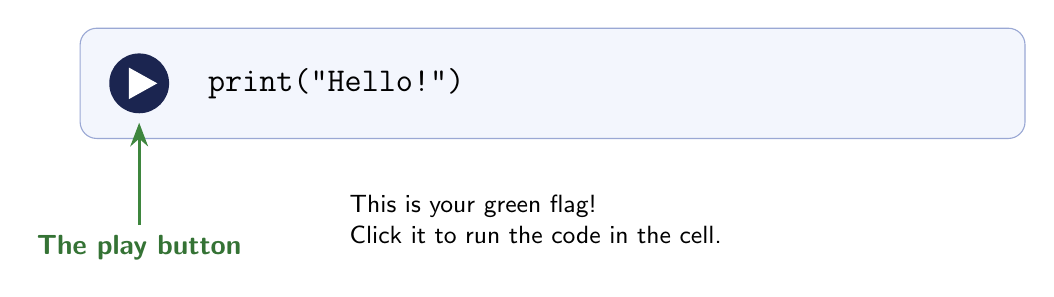
\begin{tikzpicture}
  \draw[codeframe, fill=codebg, rounded corners=6pt] (0,0) rectangle (12,1.4);
  \fill[ink] (0.75,0.7) circle (0.38);
  \fill[white] (0.62,0.5) -- (0.62,0.9) -- (0.98,0.7) -- cycle;
  \node[anchor=west, font=\ttfamily\large] at (1.5,0.7) {print("Hello!")};
  \draw[-{Stealth[length=3mm]}, line width=1.2pt, operators!70!black] (0.75,-1.1) -- (0.75,0.2);
  \node[anchor=north, font=\bfseries, text=operators!60!black] at (0.75,-1.1) {The play button};
  \node[anchor=north west, align=left, font=\small] at (3.3,-0.6) {This is your green flag!\\ Click it to run the code in the cell.};
\end{tikzpicture}
\end{center}

\step{Step 4: Say hello}
Click inside the cell and type this exactly:

\begin{typethis}
print("Hello!")
\end{typethis}

Now click the play button \playbtn. You can also hold \textbf{Shift} and press \textbf{Enter}. The first time, it may take a few seconds to start. Then you will see this underneath:

\begin{outputbox}
Hello!
\end{outputbox}

\textbf{You just ran your first Python program!}

\step{Step 5: Add more cells}
Click \textbf{+ Code} at the top to get a new empty cell. Use a new cell for each program. You can run any cell again whenever you like.

\needspace{16\baselineskip}
\subsection*{The ``In the beginning'' cell: getting the turtle}

In Scratch, you get the pen blocks by clicking the \textbf{Extensions} button in the bottom corner. Python works the same way: we add the drawing tools we need. In Python, the sprite that draws is called a \textbf{turtle}. It walks around the stage and leaves a line behind it, just like a Scratch sprite after \chip[pen]{pen down}.

Each time you open your notebook, run this cell first. We call it the \textbf{``In the beginning'' cell}. The Bible starts with ``In the beginning God created the heavens and the earth'' (Genesis 1:1), and every Colab session starts with this cell:

\begin{typethis}[The ``In the beginning'' cell: run it once every time you open Colab]
!pip install ColabTurtlePlus
\end{typethis}

The \texttt{!} at the start means: ``this isn't Python. It is an instruction for Colab to download the turtle tools.'' Lots of text will scroll past. That is fine. Wait until it stops.

\begin{watchout}[Watch out: Plus!]
It must say \textbf{ColabTurtlePlus}, with \textbf{Plus} on the end. There is a different, older library called \texttt{ColabTurtle}. It has a black stage, a different size, and (0, 0) in the wrong corner, so none of the programs in this book would work with it.
\end{watchout}

\needspace{20\baselineskip}
\subsection*{The three starting lines}

Every program that draws starts with these three lines. They do the same job as this Scratch block:\par\chip[events]{when green flag clicked}

\begin{typethis}[Start every drawing with these lines]
from ColabTurtlePlus.Turtle import *
clearscreen()
initializeTurtle((480, 360))
\end{typethis}

\begin{longtable}{>{\centering\arraybackslash}p{0.8cm} P{14.5cm}}
\toprule
\textbf{Line} & \textbf{What it does} \\
\midrule
1 & \textbf{Bring in the turtle tools.} This is like clicking Extensions and choosing Pen. The \texttt{*} means ``bring in all of them''. \\
2 & \textbf{Clear the stage.} It wipes away the old drawing and the old turtles, so you can start fresh every time you run the cell. \\
3 & \textbf{Make the stage 480 wide and 360 tall, and get the turtle ready.} That is exactly the same size as the Scratch stage! The two numbers sit in their own extra pair of brackets, \texttt{(480, 360)}, because the width and the height travel together as one thing. \\
\bottomrule
\end{longtable}

After these lines, you can just tell the turtle what to do. The turtle is like the \textbf{selected sprite} in Scratch: when you click a sprite, the blocks you snap together belong to it. In Python, you simply write \py|forward(100)|, and the turtle knows you mean it.

\needspace{14\baselineskip}
Try it! Type the three starting lines, then one more:

\begin{typethis}
from ColabTurtlePlus.Turtle import *
clearscreen()
initializeTurtle((480, 360))
forward(100)
\end{typethis}

The turtle starts in the middle of the stage, at (0, 0), facing \textbf{right}, just like a new Scratch sprite. When you run the cell, it walks 100 steps to the right and draws a line.

When you run the starting lines, Colab may also print a short note about \py|clearscreen()|. That is fine. It is just a reminder, and you can ignore it.

\begin{watchout}[If Colab gets stuck or forgets]
\begin{itemize}
  \item \textbf{A cell keeps running forever?} Click the \stopbtn{} button where the play button was. This is just like the red stop sign in Scratch.
  \item \textbf{You see \texttt{No module named 'ColabTurtlePlus'}?} Colab forgets everything when you close it or leave it alone for a while. Run the ``In the beginning'' cell again.
  \item \textbf{You see a \texttt{NameError}?} Python doesn't know a word yet, because a cell above has not run. Run the cells above it first, starting from the top. Or click \textbf{Runtime}, then \textbf{Run all}, to run every cell in order.
\end{itemize}
\end{watchout}

\begin{think}[Tip: switch on line numbers]
The line-by-line tables in this book talk about ``line 3'' and ``line 4''. Colab can number the lines in your cells too. Click \textbf{Tools}, then \textbf{Settings}, then \textbf{Editor}, and tick \textbf{Show line numbers}.
\end{think}

% =====================================================================
\banner{motion}{THE BIG PICTURE}{Scratch words, Python words}

Here are the Scratch things you know, and what Python calls them.

\begin{center}
\renewcommand{\arraystretch}{1.35}
\begin{tabular}{P{3.9cm} P{4.6cm} P{7.0cm}}
\toprule
\textbf{In Scratch} & \textbf{In Python with Colab} & \textbf{Example} \\
\midrule
The selected sprite & The turtle & \py|forward(100)| \\
Another sprite & A new turtle with its own name & \py|cat = Turtle()| \\
The stage & The drawing area & \lstinline[style=inl,basicstyle=\ttfamily\small]|initializeTurtle((480, 360))| \\
The green flag & The play button \playbtn & or Shift + Enter \\
The stop sign & The stop button \stopbtn & \\
A block & A line of code & \py|forward(10)| \\
Extensions button & \texttt{import} & \py|import random| \\
A white input bubble & Brackets \texttt{( )} & \py|right(90)| \\
Words in a bubble & Words in quote marks & \py|"Hello!"| \\
Make a Variable & Just give it a value & \py|score = 0| \\
My Blocks & A function & \py|def jump():| \\
\bottomrule
\end{tabular}
\end{center}

\begin{think}[More than one sprite]
Most programs only need the one turtle, so you just write \py|forward(100)|. When you want a second sprite, you make a new turtle and give it a name: \py|cat = Turtle()|. Then you tell that one what to do by putting its name and a dot first: \py|cat.forward(10)| means ``cat, move 10 steps''.
\end{think}

\needspace{20\baselineskip}
\subsection*{The stage is the same}

Good news: the turtle's stage has the same coordinates as the Scratch stage. The middle is (0, 0). \textbf{x} goes from −240 on the left to 240 on the right. \textbf{y} goes from −180 at the bottom to 180 at the top.

\begin{center}
\begin{tikzpicture}[scale=0.016]
  \draw[ink, line width=1pt, fill=white] (-240,-180) rectangle (240,180);
  \draw[muted!50, -{Stealth}] (-240,0) -- (255,0) node[right, font=\small, text=ink] {x};
  \draw[muted!50, -{Stealth}] (0,-180) -- (0,195) node[above, font=\small, text=ink] {y};
  \fill[motion] (0,0) circle (7);
  \node[font=\small, anchor=south west] at (5,5) {(0, 0)};
  \node[font=\small, anchor=east] at (-245,0) {−240};
  \node[font=\small, anchor=west] at (262,-18) {240};
  \node[font=\small, anchor=north] at (0,-185) {−180};
  \node[font=\small, anchor=south west] at (6,182) {180};
  \fill[looks] (100,80) circle (7) node[right, font=\small, text=ink] {\ (100, 80)};
\end{tikzpicture}
\end{center}

So \chip[motion]{go to x: 100 y: 80} is \py|goto(100, 80)|, and the turtle lands on the purple dot, the very same spot as in Scratch.

\needspace{12\baselineskip}
\subsection*{But the compass is turned!}

\begin{watchout}[Watch out: the compass is turned]
In Scratch, \chip[motion]{point in direction 90} points to the \textbf{right}, and 0 points \textbf{up}.

In Python, \py|setheading(0)| points to the \textbf{right}, and 90 points \textbf{up}.
\end{watchout}

\begin{center}
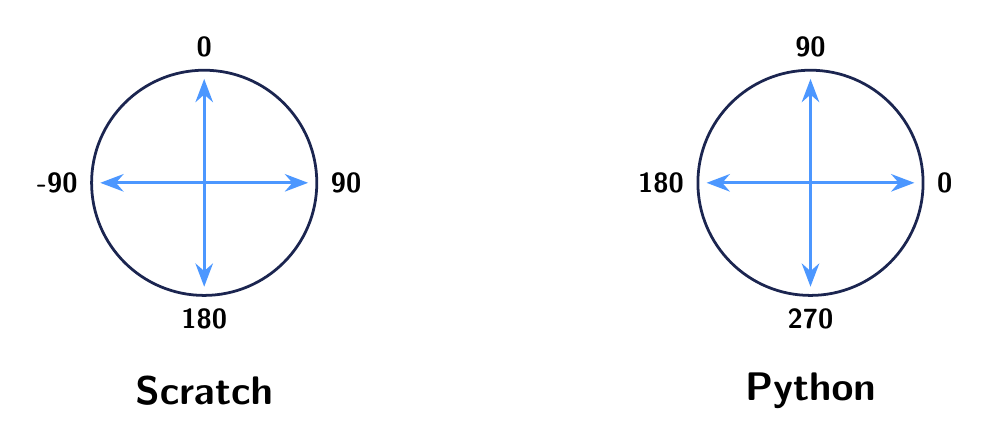
\begin{tikzpicture}[scale=1.1]
  \foreach \cx/\title/\up/\right/\down/\left in {0/Scratch/0/90/180/-90, 7/Python/90/0/270/180}{
    \begin{scope}[shift={(\cx,0)}]
      \draw[ink, line width=1pt] (0,0) circle (1.3);
      \draw[-{Stealth}, line width=1.2pt, motion] (0,0) -- (0,1.2);
      \draw[-{Stealth}, line width=1.2pt, motion] (0,0) -- (1.2,0);
      \draw[-{Stealth}, line width=1.2pt, motion] (0,0) -- (0,-1.2);
      \draw[-{Stealth}, line width=1.2pt, motion] (0,0) -- (-1.2,0);
      \node[above, font=\bfseries] at (0,1.35) {\up};
      \node[right, font=\bfseries] at (1.35,0) {\right};
      \node[below, font=\bfseries] at (0,-1.35) {\down};
      \node[left, font=\bfseries] at (-1.35,0) {\left};
      \node[font=\Large\bfseries] at (0,-2.4) {\title};
    \end{scope}}
\end{tikzpicture}
\end{center}

\begin{think}[The secret rule]
To turn any Scratch direction into a Python direction, take it away from 90:
\begin{center}\textbf{Python direction = 90 − Scratch direction}\end{center}
You don't even have to do the sum yourself. Python can do it for you!
\end{think}

\begin{tcbraster}[raster columns=2, raster equal height=rows, raster column skip=12pt, raster valign=center]
\begin{tcolorbox}[colback=white, colframe=white, boxrule=0pt, valign=center]
\begin{scratch}
\blockmove{point in direction \ovalnum{180}}
\end{scratch}
\end{tcolorbox}
\begin{code}
setheading(90 - 180)
\end{code}
\end{tcbraster}

90 − 180 is −90. Python understands −90 too: it points \textbf{down}, the same as Scratch's 180.

\begin{center}
\renewcommand{\arraystretch}{1.25}
\begin{tabular}{lll}
\toprule
\textbf{Scratch direction} & \textbf{Python} & \textbf{Points} \\
\midrule
0 & \py|setheading(90 - 0)| & up \\
90 & \py|setheading(90 - 90)| & right \\
180 & \py|setheading(90 - 180)| & down \\
−90 & \py|setheading(90 - -90)| & left \\
\bottomrule
\end{tabular}
\end{center}

The good news is that \textbf{turning} works the same. \chip[motion]{turn right 90 degrees} is \py|right(90)|, and \chip[motion]{turn left 90 degrees} is \py|left(90)|. Most of the time you will use turning, not directions.

% =====================================================================
\banner{control}{THE BIG PICTURE}{Four new habits}

Python understands the same ideas as Scratch. But because you type instead of snapping blocks, there are four new habits to learn.

\subsection*{Habit 1: Spaces show what is inside}

In Scratch, a block goes \textbf{inside} a loop when you drop it into the C-shaped mouth.

In Python, two things do that job:
\begin{enumerate}
  \item a \textbf{colon} \texttt{:} at the end of the line opens the mouth.
  \item \textbf{four spaces} at the start of a line put it inside.
\end{enumerate}

\begin{tcbraster}[raster columns=2, raster equal height=rows, raster column skip=12pt, raster valign=center]
\begin{tcolorbox}[colback=white, colframe=white, boxrule=0pt, valign=center]
\begin{scratch}
\blockrepeat{repeat \ovalnum{4}}{
  \blockmove{move \ovalnum{100} steps}
  \blockmove{turn \turnright{} \ovalnum{90} degrees}
}
\blockpen{pen up}
\end{scratch}
\end{tcolorbox}
\begin{spaces}
for i in range(4):
    forward(100)
    right(90)
penup()
\end{spaces}
\end{tcbraster}

The little \texttt{\textvisiblespace} marks show the spaces, which are normally invisible. Lines 2 and 3 have four spaces, so they are \textbf{inside} the loop and repeat 4 times. Line 4 has no spaces, so it is \textbf{outside} the loop. It happens once, after the loop has finished.

\begin{think}[Colab helps you]
When you type a colon \texttt{:} and press Enter, Colab adds the four spaces for you. To come back out of the loop, press \textbf{Backspace} once.
\end{think}

\needspace{14\baselineskip}
\subsection*{Habit 2: Spell it exactly}

Blocks are already spelled for you. In Python, you do the spelling, and Python is very fussy. Capital letters, brackets and quote marks must all be just right.

\begin{tcbraster}[raster columns=2, raster equal height=rows, raster column skip=12pt, raster valign=center]
\begin{tcolorbox}[colback=white, colframe=white, boxrule=0pt, valign=center]
\begin{scratch}
\blockmove{move \ovalnum{100} steps}
\end{scratch}
\end{tcolorbox}
\begin{code}
forward(100)
\end{code}
\end{tcbraster}

\begin{center}
\renewcommand{\arraystretch}{1.3}
\begin{tabular}{P{4.2cm} P{11cm}}
\toprule
\py|forward(100)| & \textbf{Works!} \\
\py|Forward(100)| & \textbf{Error:} capital F. Python thinks \texttt{Forward} and \texttt{forward} are different words. \\
\py|foward(100)| & \textbf{Error:} missing r. Python can't guess what you meant. \\
\py|forward 100| & \textbf{Error:} no brackets around 100. \\
\py|forward(100| & \textbf{Error:} the closing bracket is missing. \\
\py|print("Hi)| & \textbf{Error:} the closing quote mark is missing. \\
\bottomrule
\end{tabular}
\end{center}

\begin{think}[Rule of pairs]
Brackets and quotes always come in pairs, just like socks! Every \texttt{(} needs a \texttt{)}, and every \texttt{"} needs another \texttt{"}.
\end{think}

\needspace{20\baselineskip}
\subsection*{Habit 3: One line at a time, from the top}

In Scratch, you can have lots of scripts that all start when you click the green flag. They all run at the same time.

Python is different. It reads your cell like a book: line 1, then line 2, then line 3, all the way to the bottom. It only jumps around when a loop or one of your own functions tells it to.

\begin{tcbraster}[raster columns=2, raster equal height=rows, raster column skip=12pt, raster valign=center]
\begin{tcolorbox}[colback=white, colframe=white, boxrule=0pt, valign=center]
\begin{scratch}
\blockinit{when \greenflag clicked}
\blocklook{say \ovalnum{first}}
\blocklook{say \ovalnum{second}}
\blocklook{say \ovalnum{third}}
\end{scratch}
\end{tcolorbox}
\begin{code}
print("first")
print("second")
print("third")
\end{code}
\end{tcbraster}

\needspace{24\baselineskip}
\subsection*{Habit 4: One = sets, two == checks}

Scratch has two different blocks: one to \textbf{set} a variable and one to \textbf{check} whether it equals something. Python uses equals signs for both, so it needs a way to tell them apart:

\begin{itemize}
  \item \textbf{One} equals sign \texttt{=} means ``put this value in the box''. It is like \chip[variables]{set score to 0}.
  \item \textbf{Two} equals signs \texttt{==} mean ``are these the same?''. It is like the green \chip[operators]{\ = \ } block.
\end{itemize}

\begin{tcbraster}[raster columns=2, raster equal height=rows, raster column skip=12pt, raster valign=center]
\begin{tcolorbox}[colback=white, colframe=white, boxrule=0pt, valign=center]
\begin{scratch}
\blockvariable{set \selectmenu{score} to \ovalnum{5}}
\blockif{if \booloperator{\ovalvariable{score} = \ovalnum{5}} then}{
  \blocklook{say \ovalnum{You win!}}
}
\end{scratch}
\end{tcolorbox}
\begin{code}
score = 5
if score == 5:
    print("You win!")
\end{code}
\end{tcbraster}

% =====================================================================
\banner{pen}{THE BIG PICTURE}{How Colab is different from Scratch}

\subsection*{Colab asks instead of listening}

Colab can't hear key presses or mouse clicks. So instead of \chip[events]{when space key pressed}, your program \textbf{asks} you with \py|input()|, and you type your answer in a box under the cell.

\begin{typethis}
answer = input("Do you like cats? ")
if answer == "yes":
    print("Me too!")
\end{typethis}

Type \texttt{yes}, press Enter, and Python answers you. Later in the book you will meet a program that can hear keys, for real key-press games.

\subsection*{One loop moves all the sprites}

\noindent
\begin{minipage}[c]{0.64\linewidth}
\begin{typethis}[Type this]
from ColabTurtlePlus.Turtle import *
clearscreen()
initializeTurtle((480, 360))
cat = Turtle()
dog = Turtle()
dog.left(90)
for i in range(10):
    cat.forward(10)
    dog.forward(10)
\end{typethis}
\end{minipage}\hfill
\begin{minipage}[c]{0.33\linewidth}\raggedright
Python does one line at a time, so \textbf{one loop moves every sprite} a little bit each time round.

Here the cat walks right and the dog walks up. In Scratch, this would be two scripts.
\end{minipage}

\subsection*{Shapes and colours instead of costumes}

There are no costume pictures in Colab, but the turtle can wear lots of \textbf{shapes}, like \texttt{"turtle"}, \texttt{"arrow"} or \texttt{"circle"}, in any colour you like: \py|shape("turtle")| and \py|color("gold")|. (Python spells colour \texttt{color}, with no \texttt{u}, and colour names use small letters.) And it can draw anything you can imagine, line by line. \textbf{You are ready. Let's go!}

% Generated by chapters/_make_mission_chart.py -- do not edit by hand.
\banner{events}{TRACK YOUR PROGRESS}{My missions}
Colour in a star each time you finish a mission: one star for making it work, two for doing one challenge, and three for doing them all!
\begin{center}\renewcommand{\arraystretch}{1.12}
\begin{longtable}{c P{10.5cm} l}
\toprule
\textbf{Mission} & \textbf{What you make} & \textbf{Done?} \\
\midrule
\endhead
\multicolumn{3}{l}{\rule{0pt}{14pt}\textbf{Part 1: Motion and Pen}} \\
1 & A square the long way & $\star$\ \ $\star$\ \ $\star$ \\
2 & Draw a house & $\star$\ \ $\star$\ \ $\star$ \\
3 & Robot face & $\star$\ \ $\star$\ \ $\star$ \\
\multicolumn{3}{l}{\rule{0pt}{14pt}\textbf{Part 2: Loops}} \\
4 & Draw shapes the short way & $\star$\ \ $\star$\ \ $\star$ \\
5 & Stars & $\star$\ \ $\star$\ \ $\star$ \\
6 & Square spiral & $\star$\ \ $\star$\ \ $\star$ \\
7 & Flower of squares & $\star$\ \ $\star$\ \ $\star$ \\
\multicolumn{3}{l}{\rule{0pt}{14pt}\textbf{Part 3: Variables and Lists}} \\
8 & Score counter & $\star$\ \ $\star$\ \ $\star$ \\
9 & Growing spiral & $\star$\ \ $\star$\ \ $\star$ \\
10 & Rainbow from a colour list & $\star$\ \ $\star$\ \ $\star$ \\
11 & Random story maker & $\star$\ \ $\star$\ \ $\star$ \\
\multicolumn{3}{l}{\rule{0pt}{14pt}\textbf{Part 4: Operators}} \\
12 & Dice roller & $\star$\ \ $\star$\ \ $\star$ \\
13 & Times-table printer & $\star$\ \ $\star$\ \ $\star$ \\
14 & Random dot art & $\star$\ \ $\star$\ \ $\star$ \\
15 & Name machine & $\star$\ \ $\star$\ \ $\star$ \\
\multicolumn{3}{l}{\rule{0pt}{14pt}\textbf{Part 5: Sensing and Decisions}} \\
16 & Say hello & $\star$\ \ $\star$\ \ $\star$ \\
17 & Guess my number & $\star$\ \ $\star$\ \ $\star$ \\
18 & Quiz with a score & $\star$\ \ $\star$\ \ $\star$ \\
19 & Reaction timer & $\star$\ \ $\star$\ \ $\star$ \\
\multicolumn{3}{l}{\rule{0pt}{14pt}\textbf{Part 6: My Blocks}} \\
20 & Make your own block & $\star$\ \ $\star$\ \ $\star$ \\
21 & Shape machine & $\star$\ \ $\star$\ \ $\star$ \\
22 & Answer machine & $\star$\ \ $\star$\ \ $\star$ \\
23 & Sprite army & $\star$\ \ $\star$\ \ $\star$ \\
\multicolumn{3}{l}{\rule{0pt}{14pt}\textbf{Part 7: Looks, Sound and Events}} \\
24 & Costume parade & $\star$\ \ $\star$\ \ $\star$ \\
25 & Make music & $\star$\ \ $\star$\ \ $\star$ \\
26 & Turtle race & $\star$\ \ $\star$\ \ $\star$ \\
27 & Story with messages & $\star$\ \ $\star$\ \ $\star$ \\
\multicolumn{3}{l}{\rule{0pt}{14pt}\textbf{Big Projects}} \\
28 & Animate your name & $\star$\ \ $\star$\ \ $\star$ \\
29 & Pen flower & $\star$\ \ $\star$\ \ $\star$ \\
30 & Maths quiz & $\star$\ \ $\star$\ \ $\star$ \\
31 & Guess the number deluxe & $\star$\ \ $\star$\ \ $\star$ \\
32 & Choose-your-own story & $\star$\ \ $\star$\ \ $\star$ \\
33 & Virtual pet & $\star$\ \ $\star$\ \ $\star$ \\
34 & Chase game & $\star$\ \ $\star$\ \ $\star$ \\
35 & Catch game & $\star$\ \ $\star$\ \ $\star$ \\
\bottomrule
\end{longtable}
\end{center}


% =====================================================================
% PART 1: Motion and Pen
% =====================================================================
\partopener{motion}{PART 1}{Motion and Pen}{Make the turtle walk, turn and draw, just like a sprite with the Pen extension.}

In Scratch, the blue \textbf{Motion} blocks move your sprite around the stage, and the green \textbf{Pen} blocks let it draw. In Python, the \textbf{turtle} does both jobs. It is a sprite that always carries a pen.

In this part you will learn the Python for blocks like these:

{\raggedright \chip[motion]{move 10 steps} \chip[motion]{turn right 15 degrees} \chip[motion]{go to x: 0 y: 0} \chip[motion]{glide 1 secs to x: 0 y: 0} \chip[motion]{point in direction 90} \chip[motion]{change x by 10} \chip[motion]{x position} \chip[pen]{pen down} \chip[pen]{pen up} \chip[pen]{set pen color to} \chip[pen]{set pen size to 1} \chip[pen]{erase all} \chip[pen]{stamp}\par}

And you will learn some Python tricks that Scratch \textbf{can't} do, like circles, dots, filled-in shapes and writing words on the stage.

\subsection*{Before you start}

Every drawing program in this part begins with the \textbf{three starting lines}. They are like \chip[events]{when green flag clicked}. They bring in the turtle, wipe the stage and make it the same size as the Scratch stage.

\begin{typethis}[The three starting lines]
from ColabTurtlePlus.Turtle import *
clearscreen()
initializeTurtle((480, 360))
\end{typethis}

On the concept pages below, the boxes show only the new lines. Type the three starting lines first, then the new lines underneath, and press \playbtn.

\begin{think}[Where does the turtle start?]
\begin{itemize}
  \item In the middle of the stage, at $(0, 0)$, just like a new sprite.
  \item Pointing to the \textbf{right}, just like a new sprite (Scratch direction 90).
  \item With its pen \textbf{down}. This is different! A Scratch sprite only draws after \chip[pen]{pen down}, but the turtle draws a line every time it moves.
\end{itemize}
\end{think}

% ---------------------------------------------------------------------
\needspace{10\baselineskip}
\subsection*{Move and turn}

\begin{tcbraster}[raster columns=2, raster equal height=rows, raster column skip=12pt, raster valign=center]
\begin{tcolorbox}[colback=white, colframe=white, boxrule=0pt, valign=center]
\begin{scratch}
\blockmove{move \ovalnum{100} steps}
\blockmove{turn \turnright{} \ovalnum{90} degrees}
\blockmove{move \ovalnum{100} steps}
\blockmove{turn \turnleft{} \ovalnum{45} degrees}
\blockmove{move \ovalnum{-50} steps}
\end{scratch}
\end{tcolorbox}
\begin{code}
forward(100)
right(90)
forward(100)
left(45)
backward(50)
\end{code}
\end{tcbraster}

\textbf{How it works:} \py|forward(100)| is \chip[motion]{move 100 steps}. The number goes inside the round brackets \texttt{( )}, just like it goes inside the white bubble on the block. One step is one pixel in both, so your Scratch numbers work in Python too. To walk backwards, Scratch uses a minus number, but Python has its own word, \py|backward|.

\py|right(90)| turns clockwise, like the $\circlearrowright$ arrow, and \py|left(45)| turns anticlockwise, like the $\circlearrowleft$ arrow. The good news: turning works \textbf{exactly} the same in Scratch and Python.

\begin{watchout}[Watch out: lowercase only]
Python is fussy about capital letters. \py|forward(100)| works, but \py|Forward(100)| gives an error. Every command in this part is written in lowercase letters.
\end{watchout}

% ---------------------------------------------------------------------
\needspace{14\baselineskip}
\subsection*{Go to a spot}

\begin{tcbraster}[raster columns=2, raster equal height=rows, raster column skip=12pt, raster valign=center]
\begin{tcolorbox}[colback=white, colframe=white, boxrule=0pt, valign=center]
\begin{scratch}
\blockmove{go to x: \ovalnum{100} y: \ovalnum{50}}
\blockmove{go to x: \ovalnum{-100} y: \ovalnum{50}}
\blockmove{go to x: \ovalnum{0} y: \ovalnum{0}}
\end{scratch}
\end{tcolorbox}
\begin{code}
goto(100, 50)
goto(-100, 50)
goto(0, 0)
\end{code}
\end{tcbraster}

\textbf{How it works:} \py|goto(100, 50)| means ``go to x: 100, y: 50''. The x number always comes first, then a comma, then the y number. The stage is the same as in Scratch: $(0, 0)$ is the middle, x goes from $-240$ to $240$ and y goes from $-180$ to $180$. Because the pen is down, this program draws a triangle!

% ---------------------------------------------------------------------
\needspace{13\baselineskip}
\subsection*{Glide slowly}

\begin{tcbraster}[raster columns=2, raster equal height=rows, raster column skip=12pt, raster valign=center]
\begin{tcolorbox}[colback=white, colframe=white, boxrule=0pt, valign=center]
\begin{scratch}
\blockmove{glide \ovalnum{3} secs to x: \ovalnum{150} y: \ovalnum{100}}
\blockmove{glide \ovalnum{0.2} secs to x: \ovalnum{-150} y: \ovalnum{100}}
\end{scratch}
\end{tcolorbox}
\begin{code}
speed(1)
goto(150, 100)
speed(13)
goto(-150, 100)
\end{code}
\end{tcbraster}

\textbf{How it works:} The turtle always glides when it moves. You choose how fast with \py|speed()|. It takes a number from \textbf{1} (slowest, like a snail) to \textbf{13} (fastest, like a rocket). Python doesn't use seconds, so you pick the speed that looks right. The speed stays the same until you change it, so put \py|speed(13)| near the top when you want a big drawing to finish quickly.

\begin{watchout}[Watch out: don't use speed 0]
You might think \py|speed(0)| means ``stand still''. It doesn't! In Colab it means ``don't show anything until the end'', so your stage stays empty. Stick to 1 to 13.
\end{watchout}

% ---------------------------------------------------------------------
\needspace{13\baselineskip}
\subsection*{Point in a direction}

\begin{tcbraster}[raster columns=2, raster equal height=rows, raster column skip=12pt, raster valign=center]
\begin{tcolorbox}[colback=white, colframe=white, boxrule=0pt, valign=center]
\begin{scratch}
\blockmove{point in direction \ovalnum{0}}
\blockmove{move \ovalnum{100} steps}
\blockmove{point in direction \ovalnum{180}}
\blockmove{move \ovalnum{50} steps}
\end{scratch}
\end{tcolorbox}
\begin{code}
setheading(90 - 0)
forward(100)
setheading(90 - 180)
forward(50)
\end{code}
\end{tcbraster}

\textbf{How it works:} \py|setheading| means ``point in direction''. But Python's compass is turned round! In Scratch, 0 points \textbf{up} and the numbers go clockwise. In Python, 0 points \textbf{right} and the numbers go anticlockwise. Python can do sums inside the brackets, so we let it do the translating for us.

\begin{center}
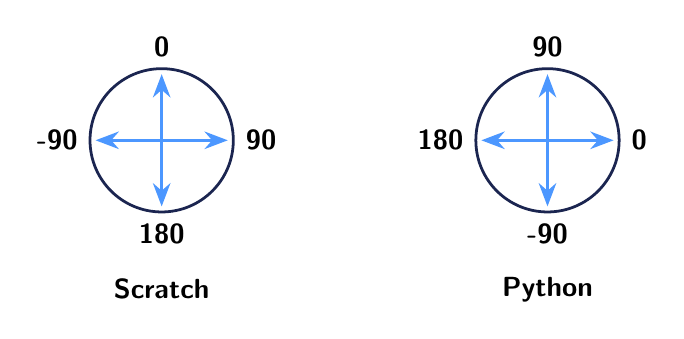
\begin{tikzpicture}[scale=0.7]
  \foreach \cx/\title/\up/\right/\down/\left in {0/Scratch/0/90/180/-90, 7/Python/90/0/-90/180}{
    \begin{scope}[shift={(\cx,0)}]
      \draw[ink, line width=1pt] (0,0) circle (1.3);
      \foreach \a in {0,90,180,270} \draw[-{Stealth}, line width=1.2pt, motion] (0,0) -- (\a:1.2);
      \node[above, font=\bfseries] at (0,1.35) {\up};
      \node[right, font=\bfseries] at (1.35,0) {\right};
      \node[below, font=\bfseries] at (0,-1.35) {\down};
      \node[left, font=\bfseries] at (-1.35,0) {\left};
      \node[font=\bfseries] at (0,-2.7) {\title};
    \end{scope}}
\end{tikzpicture}
\end{center}

\begin{think}[The secret rule]
\begin{center}\textbf{Python direction} $=$ \textbf{90} $-$ \textbf{Scratch direction}\end{center}
So \chip[motion]{point in direction 30} becomes \py|setheading(90 - 30)|. Write the Scratch number after the \texttt{90 -} and Python works out the rest. You never have to do the sum in your head!
\end{think}

\needspace{12\baselineskip}
\textbf{Fill in the table.} Work out each Python direction. Then try it in Colab with \py|forward(100)| after it, and check the turtle goes the way you expected.

\begin{center}
\renewcommand{\arraystretch}{1.5}
\begin{tabular}{P{2.8cm} P{6.0cm} P{3.0cm} P{2.8cm}}
\toprule
\textbf{Scratch direction} & \textbf{Python code} & \textbf{Python direction} & \textbf{Which way?} \\
\midrule
90 & \py|setheading(90 - 90)| & 0 & right \\
0 & \py|setheading(90 - 0)| & 90 & up \\
-90 & \py|setheading(90 - -90)| & \rule{2cm}{0.5pt} & \rule{2cm}{0.5pt} \\
45 & \py|setheading(90 - 45)| & \rule{2cm}{0.5pt} & \rule{2cm}{0.5pt} \\
135 & \py|setheading(90 - 135)| & \rule{2cm}{0.5pt} & \rule{2cm}{0.5pt} \\
\bottomrule
\end{tabular}
\end{center}

% ---------------------------------------------------------------------
\needspace{13\baselineskip}
\subsection*{Point towards something}

\begin{tcbraster}[raster columns=5, raster equal height=rows, raster column skip=12pt, raster valign=center]
\begin{tcolorbox}[raster multicolumn=2, colback=white, colframe=white, boxrule=0pt, valign=center]
\begin{scratch}
\blockmove{point towards \selectmenu{Star}}
\blockmove{move \ovalnum{100} steps}
\end{scratch}
\end{tcolorbox}
\begin{tcolorbox}[raster multicolumn=3, blank]
\begin{code}
setheading(towards(100, 100))
forward(100)
\end{code}
\end{tcolorbox}
\end{tcbraster}

\textbf{How it works:} In Scratch you point towards another sprite, like a Star sitting at x: 100, y: 100. In Python you point towards a \textbf{spot}. \py|towards(100, 100)| works out which direction the spot is in, and \py|setheading( )| turns the turtle to face it. One command sits inside the other, like a round block dropped into a white bubble.

\begin{think}[No 90 minus this time]
\py|towards| already gives the answer in Python's directions, so you don't need the secret rule here. You only need \texttt{90 -} when \textbf{you} type a Scratch direction number.
\end{think}

% ---------------------------------------------------------------------
\needspace{13\baselineskip}
\subsection*{Change x and y, set x and y}

\begin{tcbraster}[raster columns=2, raster equal height=rows, raster column skip=12pt, raster valign=center]
\begin{tcolorbox}[colback=white, colframe=white, boxrule=0pt, valign=center]
\begin{scratch}
\blockmove{change x by \ovalnum{50}}
\blockmove{change y by \ovalnum{50}}
\blockmove{set x to \ovalnum{-100}}
\blockmove{set y to \ovalnum{0}}
\end{scratch}
\end{tcolorbox}
\begin{code}
setx(xcor() + 50)
sety(ycor() + 50)
setx(-100)
sety(0)
\end{code}
\end{tcbraster}

\textbf{How it works:} \py|setx(-100)| is \chip[motion]{set x to -100}, and \py|sety(0)| is \chip[motion]{set y to 0}. Python has no ``change x'' command, so we build one. \py|xcor()| means ``my x position''. So \py|setx(xcor() + 50)| says: ``set x to (my x position + 50)''. That moves the turtle 50 steps to the right, which is exactly what \chip[motion]{change x by 50} does!

\begin{watchout}
\py|xcor()| needs its empty brackets. They tell Python ``go and get the answer now''. Without them, Python gets confused.
\end{watchout}

% ---------------------------------------------------------------------
\needspace{13\baselineskip}
\subsection*{Where am I? Which way am I facing?}

\begin{tcbraster}[raster columns=2, raster equal height=rows, raster column skip=12pt, raster valign=center]
\begin{tcolorbox}[colback=white, colframe=white, boxrule=0pt, valign=center]
\begin{scratch}
\blockmove{move \ovalnum{100} steps}
\blockmove{turn \turnleft{} \ovalnum{90} degrees}
\blocklook{say \ovalmove{x position} for \ovalnum{2} seconds}
\blocklook{say \ovalmove{y position} for \ovalnum{2} seconds}
\blocklook{say \ovalmove{direction} for \ovalnum{2} seconds}
\end{scratch}
\end{tcolorbox}
\begin{code}
forward(100)
left(90)
print(xcor())
print(ycor())
print(heading())
\end{code}
\end{tcbraster}

\textbf{How it works:} The round blocks \chip[motion]{x position}, \chip[motion]{y position} and \chip[motion]{direction} become \py|xcor()|, \py|ycor()| and \py|heading()|. \py|print( )| shows an answer underneath the cell, a bit like a sprite saying it.

\begin{outputbox}
100.0\\
0.0\\
90
\end{outputbox}

\begin{think}[Two things to spot]
\begin{itemize}
  \item \texttt{100.0} is just 100 written with a decimal point. Python likes to show positions that way.
  \item Scratch would say the direction is \textbf{0}, because the sprite points up. Python says \textbf{90}, because \py|heading()| answers in \textbf{Python} directions. To get the Scratch number, use the secret rule again: \py|print(90 - heading())|.
\end{itemize}
\end{think}

% ---------------------------------------------------------------------
\needspace{14\baselineskip}
\subsection*{Sneak peek: go to a random spot}

\begin{tcbraster}[raster columns=5, raster equal height=rows, raster column skip=12pt, raster valign=center]
\begin{tcolorbox}[raster multicolumn=2, colback=white, colframe=white, boxrule=0pt, valign=center]
\begin{scratch}
\blockmove{go to \selectmenu{random position}}
\end{scratch}
\end{tcolorbox}
\begin{tcolorbox}[raster multicolumn=3, blank]
\begin{code}
import random
goto(random.randint(-240, 240),
     random.randint(-180, 180))
\end{code}
\end{tcolorbox}
\end{tcbraster}

\textbf{How it works:} \py|import random| brings in Python's dice. \py|random.randint(-240, 240)| picks a whole number from $-240$ to $240$, so it is a surprise x. The second one picks a surprise y. The line was too long, so it carries on to the next line. Python allows that while a bracket is still open. You will meet \py|random| properly in Part 4.

% ---------------------------------------------------------------------
\needspace{10\baselineskip}
\subsection*{If on edge, bounce}

\begin{tcbraster}[raster columns=2, raster equal height=rows, raster column skip=12pt, raster valign=center]
\begin{tcolorbox}[colback=white, colframe=white, boxrule=0pt, valign=center]
\begin{scratch}
\blockmove{if on edge, bounce}
\end{scratch}
\end{tcolorbox}
\begin{tcolorbox}[colback=warnbg, colframe=warnframe, boxrule=0.6pt, arc=5pt]
Python has no command for this one.
\end{tcolorbox}
\end{tcbraster}

There is no wall around the turtle's stage. Try \py|forward(1000)|: the turtle walks right off the edge and keeps going! In \textbf{Part 5} you will build your own ``if on edge, bounce'' with an \py|if|. Then you will know the secret of what Scratch's block does.

% ---------------------------------------------------------------------
\needspace{13\baselineskip}
\subsection*{Pen up, pen down}

\begin{tcbraster}[raster columns=2, raster equal height=rows, raster column skip=12pt, raster valign=center]
\begin{tcolorbox}[colback=white, colframe=white, boxrule=0pt, valign=center]
\begin{scratch}
\blockpen{pen down}
\blockmove{move \ovalnum{50} steps}
\blockpen{pen up}
\blockmove{move \ovalnum{50} steps}
\blockpen{pen down}
\blockmove{move \ovalnum{50} steps}
\end{scratch}
\end{tcolorbox}
\begin{code}
forward(50)
penup()
forward(50)
pendown()
forward(50)
\end{code}
\end{tcbraster}

\textbf{How it works:} \py|penup()| lifts the pen off the paper, so the turtle moves without drawing. \py|pendown()| puts it back. The brackets are empty because these commands need no number, but Python still wants the brackets. They mean ``do it now!''. The turtle starts with its pen down, so the first \chip[pen]{pen down} needs no line of Python.

\begin{think}[Moving without a line]
To jump to a new place without drawing, use three lines: \py|penup()|, then \py|goto(x, y)|, then \py|pendown()|. You will use this trick a lot in the missions.
\end{think}

% ---------------------------------------------------------------------
\needspace{14\baselineskip}
\subsection*{Choose a pen colour}

\begin{tcbraster}[raster columns=2, raster equal height=rows, raster column skip=12pt, raster valign=center]
\begin{tcolorbox}[colback=white, colframe=white, boxrule=0pt, valign=center]
\begin{scratch}
\blockpen{set pen color to \ovalnum{red}}
\blockmove{move \ovalnum{100} steps}
\blockpen{set pen color to \ovalnum{orange}}
\blockmove{move \ovalnum{100} steps}
\end{scratch}
\end{tcolorbox}
\begin{code}
pencolor("red")
forward(100)
pencolor("#ff8800")
forward(100)
\end{code}
\end{tcbraster}

\textbf{How it works:} In Scratch you click a colour. In Python you type its name in \textbf{quote marks}, all in lowercase: \py|"red"|, \py|"gold"|, \py|"skyblue"|, \py|"hotpink"|. The quote marks tell Python ``this is a word, not a command''. There are 140 colour names to try!

For any colour at all, use a \textbf{hex code}, like \py|"#ff8800"| (orange). It is a \texttt{\#} and six digits or letters. The first two say how much red, the middle two how much green and the last two how much blue. \texttt{00} is none and \texttt{ff} is the most.

\begin{watchout}[Watch out: American spelling]
In this book we write ``colour'', but Python spells it the American way: \py|pencolor|, with no \texttt{u}. If you type \py|pencolour|, Python won't know the word.
\end{watchout}

% ---------------------------------------------------------------------
\needspace{10\baselineskip}
\subsection*{Pen size and erase all}

\begin{tcbraster}[raster columns=2, raster equal height=rows, raster column skip=12pt, raster valign=center]
\begin{tcolorbox}[colback=white, colframe=white, boxrule=0pt, valign=center]
\begin{scratch}
\blockpen{set pen size to \ovalnum{10}}
\blockmove{move \ovalnum{100} steps}
\blockpen{erase all}
\end{scratch}
\end{tcolorbox}
\begin{code}
pensize(10)
forward(100)
clear()
\end{code}
\end{tcbraster}

\textbf{How it works:} A bigger number in \py|pensize| gives a fatter line. The turtle starts at size 1, just like Scratch. The size must be more than 0: \py|pensize(0)| gives an error.

\py|clear()| rubs out everything the turtle has drawn. The turtle stays where it is, and keeps its colour and size, just like \chip[pen]{erase all}. (The starting line \py|clearscreen()| is the bigger eraser that wipes the whole stage and starts again.)

% ---------------------------------------------------------------------
\needspace{13\baselineskip}
\subsection*{Stamp}

\begin{tcbraster}[raster columns=2, raster equal height=rows, raster column skip=12pt, raster valign=center]
\begin{tcolorbox}[colback=white, colframe=white, boxrule=0pt, valign=center]
\begin{scratch}
\blockpen{stamp}
\blockmove{move \ovalnum{100} steps}
\blockpen{stamp}
\end{scratch}
\end{tcolorbox}
\begin{code}
shape("turtle")
stamp()
forward(100)
stamp()
\end{code}
\end{tcbraster}

\textbf{How it works:} \py|stamp()| prints a copy of the turtle onto the stage, like a rubber stamp. In Scratch the stamp looks like your costume. In Python it looks like the turtle's \textbf{shape}. \py|shape("turtle")| makes it look like a real turtle. You can also try the shapes \texttt{arrow}, \texttt{circle}, \texttt{square}, \texttt{triangle} and \texttt{classic} (the arrow it starts with). Remember the quote marks!

% ---------------------------------------------------------------------
\needspace{18\baselineskip}
\subsection*{Python superpowers that Scratch doesn't have}

Scratch's Pen can only draw lines. The turtle can do more!

\begin{center}
\renewcommand{\arraystretch}{1.4}
\begin{tabular}{P{5.4cm} P{10.4cm}}
\toprule
\textbf{Python} & \textbf{What it does} \\
\midrule
\py|circle(50)| & Draws a whole circle with a radius of 50 (that is the distance from the middle to the edge). The middle of the circle is on the turtle's \textbf{left}. A minus number, \py|circle(-50)|, puts it on the right. \\
\py|dot(30, "gold")| & Draws a filled-in dot, 30 across, right where the turtle is. It works even when the pen is up. \\
\py|fillcolor("skyblue")|\newline \py|begin_fill()|\newline \ldots\newline \py|end_fill()| & Colours in a shape. Choose the colour, say \py|begin_fill()|, draw the shape, then say \py|end_fill()|. The inside gets painted. \\
\py|write("Hi!")| & Writes words on the stage where the turtle is. \\
\py|shape("turtle")| & Changes how the turtle looks. A bit like choosing a costume. \\
\bottomrule
\end{tabular}
\end{center}

\needspace{12\baselineskip}
Try them all at once:

\begin{tcbraster}[raster columns=2, raster equal height=rows, raster column skip=12pt, raster valign=center]
\begin{code}
shape("turtle")
circle(50)
dot(30, "gold")
fillcolor("skyblue")
begin_fill()
circle(-40)
end_fill()
write("Hi!")
\end{code}
\begin{tcolorbox}[colback=white, colframe=white, boxrule=0pt, valign=center]
You should see an empty circle above the turtle, a blue filled-in circle below it, a gold dot where they touch, and the word \texttt{Hi!} on top. It looks a bit like a snowman!
\end{tcolorbox}
\end{tcbraster}

% =====================================================================
\mission{A square the long way}{\texttt{forward}, \texttt{right}, \texttt{pencolor}, \texttt{pensize} and \texttt{shape}, all in one program}

Time to put the blocks together. You will draw a blue square, one side at a time.

\step{Step 1: Build it in Scratch}
Add the \textbf{Pen} extension, then build:

\begin{center}
\begin{tabular}{c@{\hspace{1cm}}c}
\begin{scratch}
\blockinit{when \greenflag clicked}
\blockpen{erase all}
\blockpen{pen down}
\blockpen{set pen color to \ovalnum{blue}}
\blockpen{set pen size to \ovalnum{3}}
\blockmove{move \ovalnum{100} steps}
\blockmove{turn \turnright{} \ovalnum{90} degrees}
\end{scratch}
&
\begin{scratch}
\blockmove{move \ovalnum{100} steps}
\blockmove{turn \turnright{} \ovalnum{90} degrees}
\blockmove{move \ovalnum{100} steps}
\blockmove{turn \turnright{} \ovalnum{90} degrees}
\blockmove{move \ovalnum{100} steps}
\blockmove{turn \turnright{} \ovalnum{90} degrees}
\end{scratch}
\end{tabular}
\end{center}
The right-hand blocks join on underneath the left-hand ones.

\step{Step 2: Type it in Colab}

\begin{typethis}
from ColabTurtlePlus.Turtle import *
clearscreen()
initializeTurtle((480, 360))
shape("turtle")
pencolor("blue")
pensize(3)
forward(100)
right(90)
forward(100)
right(90)
forward(100)
right(90)
forward(100)
right(90)
\end{typethis}

\step{Step 3: Read it line by line}

\begin{longtable}{>{\centering\arraybackslash}p{1.1cm} P{5.3cm} P{9.1cm}}
\toprule
\textbf{Line} & \textbf{Scratch block} & \textbf{What it means} \\
\midrule
1--3 & \chip[events]{when green flag clicked} \chip[pen]{erase all} & The three starting lines. \py|clearscreen()| wipes the stage, so it does the job of \chip[pen]{erase all} too. \\
--- & \chip[pen]{pen down} & No line needed. The turtle's pen starts down. \\
4 & (choosing a costume) & \py|shape("turtle")| makes the turtle look like a turtle. \\
5 & \chip[pen]{set pen color to blue} & The colour name goes in quote marks. \\
6 & \chip[pen]{set pen size to 3} & A slightly fatter line. \\
7--8 & \chip[motion]{move 100 steps} \chip[motion]{turn right 90 degrees} & The first side, then a turn at the corner. \\
9--10 & the same again & The second side. \\
11--12 & the same again & The third side. \\
13--14 & the same again & The fourth side. The last turn makes the turtle face the way it started. \\
\bottomrule
\end{longtable}

\step{Step 4: Run it}
Press \playbtn. The turtle walks right, turns, walks down, and so on. You should see a blue square below the middle of the stage, with the turtle back where it started, facing right.

\begin{think}[Phew, that was long!]
Lines 7 and 8 are typed \textbf{four times}. In Scratch you would use \chip[control]{repeat 4} so you only build them once. Python has a shortcut just like that, and \textbf{Part 2} shows you how. For now, typing it the long way helps you see every step.
\end{think}

\step{Step 5: Make it yours}

\begin{challenge}
\tick Change \py|"blue"| to your favourite colour, and the pen size to 8.\par
\tick Make a bigger square: change all four \texttt{100}s to \texttt{150}.\par
\tick Make each side a different colour. Add a \py|pencolor(...)| line before each \py|forward|.\par
\tick Change every \py|right| to \py|left|. Where does the square go now? Predict first, then run it.
\end{challenge}

% =====================================================================
\mission{Draw a house}{moving without drawing with \texttt{penup} and \texttt{goto}, and filling shapes with colour}

Now you will draw a house with a roof, a door and a round window. You will use \py|goto| for every corner, and \py|penup()| to move between the parts without leaving a line.

\step{Step 1: Build it in Scratch}
Scratch can't fill shapes with colour, so the Scratch house is just outlines. Here are the walls and the roof:

\begin{center}
\begin{tabular}{c@{\hspace{1cm}}c}
\begin{scratch}
\blockinit{when \greenflag clicked}
\blockpen{erase all}
\blockpen{set pen size to \ovalnum{3}}
\blockpen{pen up}
\blockmove{go to x: \ovalnum{-100} y: \ovalnum{-150}}
\blockpen{pen down}
\blockmove{go to x: \ovalnum{100} y: \ovalnum{-150}}
\blockmove{go to x: \ovalnum{100} y: \ovalnum{50}}
\blockmove{go to x: \ovalnum{-100} y: \ovalnum{50}}
\blockmove{go to x: \ovalnum{-100} y: \ovalnum{-150}}
\end{scratch}
&
\begin{scratch}
\blockpen{pen up}
\blockmove{go to x: \ovalnum{-120} y: \ovalnum{50}}
\blockpen{pen down}
\blockmove{go to x: \ovalnum{120} y: \ovalnum{50}}
\blockmove{go to x: \ovalnum{0} y: \ovalnum{150}}
\blockmove{go to x: \ovalnum{-120} y: \ovalnum{50}}
\end{scratch}
\end{tabular}
\end{center}

The right-hand blocks join on underneath the left-hand ones. The door works the same way.

\step{Step 2: Type it in Colab}
The empty lines split the program into parts: walls, roof, door and window. Python doesn't mind empty lines, and they make it easier to read.

\begin{typethis}
from ColabTurtlePlus.Turtle import *
clearscreen()
initializeTurtle((480, 360))
speed(8)
pensize(3)
\end{typethis}
\begin{tcbraster}[raster columns=2, raster column skip=10pt, raster valign=top]
\begin{tcblisting}{listing only, enhanced, colback=codebg, colframe=codeframe, boxrule=0.8pt, arc=6pt, left=22pt, right=8pt, top=4pt, bottom=4pt, title={\textbf{\ldots and carry on in the same cell}}, coltitle=white, colbacktitle=ink, fonttitle=\small, listing options={style=py, firstnumber=7}}
penup()
goto(-100, -150)
pendown()
fillcolor("tan")
begin_fill()
goto(100, -150)
goto(100, 50)
goto(-100, 50)
goto(-100, -150)
end_fill()

penup()
goto(-120, 50)
pendown()
fillcolor("firebrick")
begin_fill()
goto(120, 50)
goto(0, 150)
goto(-120, 50)
end_fill()
\end{tcblisting}
\begin{tcblisting}{listing only, enhanced, colback=codebg, colframe=codeframe, boxrule=0.8pt, arc=6pt, left=22pt, right=8pt, top=4pt, bottom=4pt, title={\textbf{\ldots and carry on in the same cell}}, coltitle=white, colbacktitle=ink, fonttitle=\small, listing options={style=py, firstnumber=28}}
penup()
goto(-25, -150)
pendown()
fillcolor("saddlebrown")
begin_fill()
goto(-25, -70)
goto(25, -70)
goto(25, -150)
end_fill()

penup()
goto(55, -10)
dot(40, "skyblue")
hideturtle()
\end{tcblisting}
\end{tcbraster}

\step{Step 3: Read it line by line}

\begin{longtable}{>{\centering\arraybackslash}p{1.1cm} P{5.3cm} P{9.1cm}}
\toprule
\textbf{Line} & \textbf{Scratch block} & \textbf{What it means} \\
\midrule
1--3 & \chip[events]{when green flag clicked} & The three starting lines. \\
4 & (none) & \py|speed(8)| makes the turtle quicker, so you don't wait too long. \\
5 & \chip[pen]{set pen size to 3} & Fatter lines for the outline. \\
7--9 & \chip[pen]{pen up} \chip[motion]{go to x: -100 y: -150} \chip[pen]{pen down} & The ``moving without a line'' trick. The turtle hops to the bottom-left corner of the walls. \\
10--16 & \chip[motion]{go to x: 100 y: -150} and the other corners & Choose the paint colour and say \py|begin_fill()|: ``start remembering this shape''. Walk round the four corners and back to the start. Then \py|end_fill()| paints the inside tan. Scratch can't fill! \\
18--26 & the roof & The same pattern again: hop, choose a colour, draw three corners, fill. A triangle only needs three corners! \\
28--36 & the door & The same pattern a third time. The door starts at the bottom of the walls. \\
38--41 & \chip[looks]{hide} & Hop to the window spot and drop a big blue dot. Then \py|hideturtle()| hides the turtle so you can admire your house. \\
\bottomrule
\end{longtable}

\step{Step 4: Run it}
You should see a tan house with a red roof, a brown door and a round blue window.

\begin{watchout}[If a line goes across your house]
You probably forgot a \py|penup()|, so the turtle drew a line as it moved. Check lines 7, 18, 28 and 38.
\end{watchout}

\step{Step 5: Make it yours}

\begin{challenge}
\tick Paint your house in your own colours.\par
\tick Add a second window on the left. Copy lines 38 to 40 to the end, and change the x number.\par
\tick Add a sun in the top corner: hop to \py|goto(-190, 140)| and use a big \mbox{\texttt{dot(60, "gold")}}.\par
\tick Write your house number on the door. Hop to the door, then use \py|write("12")|.
\end{challenge}

% =====================================================================
\mission{Robot face}{\texttt{circle}, \texttt{dot}, \texttt{write} and \texttt{stamp}: the Python superpowers}

Meet Robo! You will draw a robot head with a round face, big eyes, a mouth and an antenna. Then Robo gets a little pet turtle.

\step{Step 1: Build it in Scratch}
Scratch has no circle block, so the head and eyes are hard to make in Scratch. Here is the part Scratch \textbf{can} do: the mouth, the antenna and the pet.

\begin{center}
\begin{tabular}{c@{\hspace{1cm}}c}
\begin{scratch}
\blockinit{when \greenflag clicked}
\blockpen{erase all}
\blockpen{set pen size to \ovalnum{4}}
\blockpen{pen up}
\blockmove{go to x: \ovalnum{-50} y: \ovalnum{-40}}
\blockpen{pen down}
\blockpen{set pen color to \ovalnum{red}}
\blockmove{go to x: \ovalnum{50} y: \ovalnum{-40}}
\end{scratch}
&
\begin{scratch}
\blockpen{pen up}
\blockmove{go to x: \ovalnum{0} y: \ovalnum{100}}
\blockpen{pen down}
\blockpen{set pen color to \ovalnum{grey}}
\blockmove{go to x: \ovalnum{0} y: \ovalnum{140}}
\blockpen{pen up}
\blockmove{go to x: \ovalnum{-150} y: \ovalnum{-120}}
\blockpen{stamp}
\blocklook{hide}
\end{scratch}
\end{tabular}
\end{center}

\step{Step 2: Type it in Colab}

\begin{typethis}
from ColabTurtlePlus.Turtle import *
clearscreen()
initializeTurtle((480, 360))
speed(10)
pensize(4)
pencolor("slategray")
\end{typethis}
\begin{tcbraster}[raster columns=2, raster column skip=10pt, raster valign=top]
\begin{tcblisting}{listing only, enhanced, colback=codebg, colframe=codeframe, boxrule=0.8pt, arc=6pt, left=22pt, right=8pt, top=4pt, bottom=4pt, title={\textbf{\ldots and carry on in the same cell}}, coltitle=white, colbacktitle=ink, fonttitle=\small, listing options={style=py, firstnumber=8}}
penup()
goto(0, -100)
pendown()
fillcolor("lightgray")
begin_fill()
circle(100)
end_fill()

penup()
goto(-40, 30)
dot(40, "white")
dot(16, "black")
goto(40, 30)
dot(40, "white")
dot(16, "black")
\end{tcblisting}
\begin{tcblisting}{listing only, enhanced, colback=codebg, colframe=codeframe, boxrule=0.8pt, arc=6pt, left=22pt, right=8pt, top=4pt, bottom=4pt, title={\textbf{\ldots and carry on in the same cell}}, coltitle=white, colbacktitle=ink, fonttitle=\small, listing options={style=py, firstnumber=24}}
goto(-50, -40)
pendown()
pencolor("red")
goto(50, -40)

penup()
goto(0, 100)
pendown()
pencolor("slategray")
goto(0, 140)
dot(20, "gold")

penup()
goto(120, -150)
write("I am Robo!")
shape("turtle")
color("seagreen")
goto(-150, -120)
stamp()
hideturtle()
\end{tcblisting}
\end{tcbraster}

\step{Step 3: Read it line by line}

\begin{longtable}{>{\centering\arraybackslash}p{1.1cm} P{5.3cm} P{9.1cm}}
\toprule
\textbf{Line} & \textbf{Scratch block} & \textbf{What it means} \\
\midrule
1--3 & \chip[events]{when green flag clicked} & The three starting lines. \\
4--6 & \chip[pen]{set pen size to 4} \chip[pen]{set pen color to} & Fast drawing, a thick line and a grey-blue colour called \py|"slategray"|. \\
8--10 & \chip[pen]{pen up} \chip[motion]{go to x: 0 y: -100} \chip[pen]{pen down} & Hop to the bottom of where the face will be. \\
11--14 & (Scratch can't do this) & \py|circle(100)| draws the face. The middle of the circle is 100 steps to the turtle's left. The turtle faces right, so its left is \textbf{up}, and the middle lands at $(0, 0)$. The fill paints it light grey. \\
16--22 & \chip[pen]{pen up} \chip[motion]{go to x: -40 y: 30} & Hop to the left eye. A big white dot with a small black dot on top makes an eyeball. Then the same for the right eye. Dots work with the pen up. \\
24--27 & \chip[motion]{go to x: -50 y: -40} \ldots & The mouth: pen down, red, and a straight line across. \\
29--34 & \chip[motion]{go to x: 0 y: 100} \ldots & The antenna: a short line up from the top of the head, and a gold dot on the end. \\
36--38 & (Scratch can't do this) & Hop below the face and \py|write| a message. Words go in quote marks. \\
39--40 & (choosing a costume) & Turn into a turtle shape. \py|color("seagreen")| sets the pen colour \textbf{and} the fill colour at once, so the turtle becomes green. \\
41--42 & \chip[motion]{go to x: -150 y: -120} \chip[pen]{stamp} & Walk to the bottom-left and stamp a copy of the turtle: Robo's pet! \\
43 & \chip[looks]{hide} & Hide the real turtle. The stamp stays behind. \\
\bottomrule
\end{longtable}

\step{Step 4: Run it}
You should see a grey round robot face with two big eyes, a straight red mouth and an antenna with a gold ball on top. ``I am Robo!'' is written in the bottom-right, and a green turtle stamp sits in the bottom-left.


\step{Step 5: Make it yours}

\begin{challenge}
\tick Give Robo different coloured eyes, like \py|"lime"| or \py|"hotpink"|.\par
\tick Change the message to your own robot's name.\par
\tick Make a smile: replace line 27 with \py|goto(0, -60)| and add \py|goto(50, -40)| after it. Now the mouth is a V shape.\par
\tick Stamp a whole family of pets. After line 42, add more \py|goto(...)| and \py|stamp()| pairs. Try changing \py|color(...)| between stamps.
\end{challenge}

% =====================================================================
\needspace{20\baselineskip}
\subsection*{Translate it yourself}

Here is a Scratch script you haven't seen. Write the Python for it on the lines below. Start with the three starting lines. Then type it into Colab to check. Hints: remember the secret rule for \chip[motion]{point in direction}, and remember that the turtle's pen starts down. (The answer is at the back of the book.)

\begin{tcbraster}[raster columns=2, raster equal height=rows, raster column skip=12pt, raster valign=center]
\begin{tcolorbox}[colback=white, colframe=white, boxrule=0pt, valign=center]
\begin{scratch}
\blockinit{when \greenflag clicked}
\blockpen{pen up}
\blockmove{go to x: \ovalnum{-100} y: \ovalnum{0}}
\blockpen{pen down}
\blockpen{set pen color to \ovalnum{red}}
\blockpen{set pen size to \ovalnum{4}}
\blockmove{point in direction \ovalnum{0}}
\blockmove{move \ovalnum{80} steps}
\blockmove{turn \turnright{} \ovalnum{90} degrees}
\blockmove{move \ovalnum{80} steps}
\blockpen{stamp}
\end{scratch}
\end{tcolorbox}
\begin{tcolorbox}[colback=white, colframe=codeframe, arc=5pt, title=\textbf{My Python}, coltitle=ink, colbacktitle=codebg]
\vspace{4pt}
\foreach \n in {1,...,13}{\rule{\linewidth}{0.4pt}\par\vspace{9pt}}
\end{tcolorbox}
\end{tcbraster}


% =====================================================================
\needspace{12\baselineskip}
\begin{puzzle}
The turtle is in the middle, facing right, as always. Make it point \textbf{straight down} and walk \textbf{100 steps}. You may use only \textbf{two lines} of Python after the three starting lines. (Hint: Scratch's direction for down is 180.)

\vspace{6pt}
\rule{\linewidth}{0.4pt}\par\vspace{12pt}
\rule{\linewidth}{0.4pt}
\end{puzzle}

% =====================================================================
\needspace{14\baselineskip}
\subsection*{Part 1 checklist}

Tick each one you can do.

\tick I can move the turtle with \py|forward| and \py|backward|, and turn it with \py|right| and \py|left|.\par
\tick I can send the turtle to a spot with \py|goto(x, y)|, and choose how fast it goes with \py|speed|.\par
\tick I can turn a Scratch direction into Python with \py|setheading(90 - d)|.\par
\tick I can move without drawing using \py|penup()| and \py|pendown()|.\par
\tick I can choose a pen colour and size, \py|clear()| the drawing and \py|stamp()| the turtle.\par
\tick I can use a Python superpower: \py|circle|, \py|dot|, \py|begin_fill| or \py|write|.

% =====================================================================
% PART 2: Loops
% =====================================================================
\partopener{control}{PART 2}{Loops}{Make the computer do the repeating for you.}

In Part 1 you drew pictures one command at a time. To draw a square you typed \py|forward(100)| and \py|right(90)| four times each. That is a lot of typing! In Scratch you would never do that. You would grab a \chip[control]{repeat 4} block and let it do the work.

In this part you will learn the Python for the orange \textbf{Control} blocks that repeat and wait:

\begin{center}
\chip[control]{repeat 10}\quad \chip[control]{forever}\quad \chip[control]{wait 1 seconds}\quad \chip[control]{stop this script}
\end{center}

By the end you will draw stars, spirals and flowers with just a few lines of code.

% ---------------------------------------------------------------------
\needspace{14\baselineskip}
\subsection*{Repeat becomes \texttt{for}}

Here is the square from Part 1, but with a loop. Look at the two sides and match each block to its line. (In this part, the side-by-side pictures leave out the three starting lines to save space. When you type a drawing program into Colab, always start with them.)

\begin{tcbraster}[raster columns=2, raster equal height=rows, raster column skip=12pt, raster valign=center]
\begin{tcolorbox}[colback=white, colframe=white, boxrule=0pt, valign=center]
\begin{scratch}[scale=0.85]
\blockinit{when \greenflag clicked}
\blockrepeat{repeat \ovalnum{4}}{
  \blockmove{move \ovalnum{100} steps}
  \blockmove{turn \turnright{} \ovalnum{90} degrees}
}
\end{scratch}
\end{tcolorbox}
\begin{code}
for i in range(4):
    forward(100)
    right(90)
\end{code}
\end{tcbraster}

\textbf{How it works.} Line 1, \py|for i in range(4):|, is the \chip[control]{repeat 4} block. You can read it as ``for each turn, 4 times''. The word \py|range(4)| means ``count 4 times''. Lines 2 and 3 are the blocks inside the loop, so they happen 4 times.

% ---------------------------------------------------------------------
\needspace{14\baselineskip}
\subsection*{The mouth of the C: a colon and four spaces}

In Scratch, a block goes \textbf{inside} a loop when you drop it into the C-shaped mouth. Python has no C shape, so it uses two things instead:

\begin{enumerate}
  \item A \textbf{colon} \texttt{:} at the end of the \py|for| line. The colon \textbf{opens the mouth}. It says ``the inside starts on the next line''.
  \item \textbf{Four spaces} at the start of a line. Those lines are \textbf{inside} the mouth.
\end{enumerate}

The first line that goes back to the left edge, with no spaces, is the block snapped \textbf{under} the C. It runs once, after the loop has finished.

\begin{tcbraster}[raster columns=2, raster equal height=rows, raster column skip=12pt, raster valign=center]
\begin{tcolorbox}[colback=white, colframe=white, boxrule=0pt, valign=center]
\begin{scratch}[scale=0.85]
\blockrepeat{repeat \ovalnum{4}}{
  \blockmove{move \ovalnum{100} steps}
  \blockmove{turn \turnright{} \ovalnum{90} degrees}
}
\blocklook{say \ovalnum{Square done!}}
\end{scratch}
\end{tcolorbox}
\begin{spaces}
for i in range(4):
    forward(100)
    right(90)
print("Square done!")
\end{spaces}
\end{tcbraster}

The little \texttt{\textvisiblespace} marks show the spaces, which are normally invisible. Lines 2 and 3 have four spaces, so they repeat 4 times. Line 4 has no spaces, so it is outside the loop. You see \texttt{Square done!} only once, when the square is finished.

\begin{think}[Colab helps you]
When you type the colon and press \textbf{Enter}, Colab puts the four spaces in for you. To come back out of the loop, press \textbf{Backspace} once at the start of the line.
\end{think}

% ---------------------------------------------------------------------
\needspace{12\baselineskip}
\subsection*{What does \texttt{i} count?}

The \texttt{i} in \py|for i in range(4):| is a \textbf{counter}. Each time the loop goes round, Python changes \texttt{i} by itself. Scratch's \chip[control]{repeat} block has no counter you can see. In Scratch you would have to make one yourself.

Let's peek at \texttt{i}. This program doesn't draw, so it doesn't need the three starting lines.

\begin{tcbraster}[raster columns=2, raster equal height=rows, raster column skip=12pt, raster valign=center]
\begin{code}
for i in range(4):
    print(i)
\end{code}
\begin{outputbox}
0\\
1\\
2\\
3
\end{outputbox}
\end{tcbraster}

Python starts counting at \textbf{0}, so \texttt{i} is 0, then 1, then 2, then 3. That is still 4 times round! Notice that \py|range(4)| stops \textbf{before} it gets to 4. You don't have to use \texttt{i}, but it is always there if you want it.

% ---------------------------------------------------------------------
\needspace{12\baselineskip}
\subsection*{Using \texttt{i} inside the loop}

Because \texttt{i} changes every time round, you can use it to make each turn of the loop a little different. The star \texttt{*} means \textbf{times} in Python (there is no $\times$ key on the keyboard).

\begin{tcbraster}[raster columns=2, raster equal height=rows, raster column skip=12pt, raster valign=center]
\begin{code}
for i in range(5):
    print(i * 10)
\end{code}
\begin{outputbox}
0\\
10\\
20\\
30\\
40
\end{outputbox}
\end{tcbraster}

Now imagine \py|forward(i * 5)| instead of \py|print(i * 10)|. The turtle would walk a bit further each time round. That is how you will draw a spiral in a mission soon! A name like \texttt{i} that holds a number is called a \textbf{variable}. You will make your own variables in Part 3.

% ---------------------------------------------------------------------
\needspace{14\baselineskip}
\subsection*{When the spaces go wrong}

Python is fussy about the colon and the spaces. Here are the two red messages you will see most often. Read them like a detective's clue note: the last line tells you what is wrong.

\textbf{Forgot the colon?}

\begin{codenonum}
for i in range(3)
    print("hi")
\end{codenonum}
\begin{errorbox}
SyntaxError: expected ':'
\end{errorbox}

Python wants the colon that opens the mouth. Add \texttt{:} to the end of the \py|for| line.

\needspace{10\baselineskip}
\textbf{Forgot the spaces?}

\begin{codenonum}
for i in range(3):
print("hi")
\end{codenonum}
\begin{errorbox}
IndentationError: expected an indented block after 'for' statement on line 1
\end{errorbox}

This means ``the C has an empty mouth''. Nothing is inside the loop. Put four spaces in front of \py|print("hi")|.

\needspace{16\baselineskip}
\begin{watchout}[Watch out: the sneaky bug with no red writing]
What if only \textbf{one} line loses its spaces?
\begin{codenonum}
for i in range(4):
    forward(100)
right(90)
\end{codenonum}
Python is happy, so there is \textbf{no error}. But \py|right(90)| is now outside the loop, like a block dropped \textbf{under} the C instead of inside it. The turtle walks forward 4 times in a row (one long line that runs off the stage) and turns only once, at the very end. If your drawing looks wrong, check the spaces first!
\end{watchout}

% ---------------------------------------------------------------------
\needspace{14\baselineskip}
\subsection*{A loop inside a loop}

In Scratch you can put a \chip[control]{repeat} block inside another \chip[control]{repeat} block. Python can do the same. The inside loop gets \textbf{more} spaces.

\begin{tcbraster}[raster columns=2, raster equal height=rows, raster column skip=12pt, raster valign=center]
\begin{tcolorbox}[colback=white, colframe=white, boxrule=0pt, valign=center]
\begin{scratch}[scale=0.85]
\blockrepeat{repeat \ovalnum{6}}{
  \blockrepeat{repeat \ovalnum{3}}{
    \blockmove{move \ovalnum{80} steps}
    \blockmove{turn \turnright{} \ovalnum{120} degrees}
  }
  \blockmove{turn \turnright{} \ovalnum{60} degrees}
}
\end{scratch}
\end{tcolorbox}
\begin{spaces}
for i in range(6):
    for j in range(3):
        forward(80)
        right(120)
    right(60)
\end{spaces}
\end{tcbraster}

\textbf{How it works.} Count the spaces at the start of each line:
\begin{itemize}
  \item \textbf{0 spaces} (line 1): the outside loop. It goes round 6 times.
  \item \textbf{4 spaces} (lines 2 and 5): inside the outside loop.
  \item \textbf{8 spaces} (lines 3 and 4): inside \textbf{both} loops. They draw one triangle.
\end{itemize}
Line 5 has 4 spaces, so it is not part of the triangle. It turns the turtle a little after each triangle. The inside loop uses a different counter letter, \texttt{j}, so the two counters don't get mixed up. The result is 6 triangles spinning round the middle, 18 lines in all.

% ---------------------------------------------------------------------
\needspace{14\baselineskip}
\subsection*{Forever becomes \texttt{while True}}

The \chip[control]{forever} block repeats with no end. In Python it is \py|while True:|. Read it as ``keep going while true is true'', and true is always true!

\begin{tcbraster}[raster columns=2, raster equal height=rows, raster column skip=12pt, raster valign=center]
\begin{tcolorbox}[colback=white, colframe=white, boxrule=0pt, valign=center]
\begin{scratch}[scale=0.85]
\blockinit{when \greenflag clicked}
\blockinfloop{forever}{
  \blockmove{move \ovalnum{100} steps}
  \blockmove{turn \turnright{} \ovalnum{90} degrees}
}
\end{scratch}
\end{tcolorbox}
\begin{code}
while True:
    forward(100)
    right(90)
\end{code}
\end{tcbraster}

\textbf{How it works.} The colon and the four spaces work just like in a \py|for| loop. The difference is that this loop \textbf{never stops on its own}. The turtle draws the same square again and again, and the cell keeps running. While a cell is running, its play button turns into a spinning circle. Click it (\stopbtn) to stop the cell, just like the red stop sign in Scratch. You can also use the menu: \textbf{Runtime}, then \textbf{Interrupt execution}.

\begin{watchout}[Watch out: forever means forever]
When you stop the cell, Colab shows some red writing that ends with \texttt{KeyboardInterrupt}. That is not a mistake. It just means ``you pressed stop''. While a forever loop is running, no other cell can run, so remember to stop it. For drawings, a \py|for| loop with a number is usually better: it finishes by itself, and you still see the whole picture.
\end{watchout}

% ---------------------------------------------------------------------
\needspace{14\baselineskip}
\subsection*{Wait becomes \texttt{time.sleep}}

The \chip[control]{wait 1 seconds} block pauses the script. Python keeps its clock in a toolbox called \py|time|. You open the toolbox once, at the top, with \py|import time|. Then \py|time.sleep(2)| means ``sleep for 2 seconds''.

\begin{tcbraster}[raster columns=2, raster equal height=rows, raster column skip=12pt, raster valign=center]
\begin{tcolorbox}[colback=white, colframe=white, boxrule=0pt, valign=center]
\begin{scratch}[scale=0.85]
\blockinit{when \greenflag clicked}
\blocklook{say \ovalnum{Ready...}}
\blockcontrol{wait \ovalnum{2} seconds}
\blocklook{say \ovalnum{Go!}}
\end{scratch}
\end{tcolorbox}
\begin{code}
import time
print("Ready...")
time.sleep(2)
print("Go!")
\end{code}
\end{tcbraster}

The dot in \py|time.sleep| means ``the \texttt{sleep} tool from the \texttt{time} toolbox''. If you forget line 1, Python gives a \texttt{NameError}, because it doesn't know what \texttt{time} is yet.

\needspace{12\baselineskip}
\textbf{Countdown rocket.} Here a loop and a wait work together. Each time round, \py|5 - i| works out the next number: $5-0=5$, then $5-1=4$, and so on.

\begin{tcbraster}[raster columns=2, raster equal height=rows, raster column skip=12pt, raster valign=center]
\begin{code}
import time
for i in range(5):
    print(5 - i)
    time.sleep(1)
print("Blast off!")
\end{code}
\begin{outputbox}
5\\
4\\
3\\
2\\
1\\
Blast off!
\end{outputbox}
\end{tcbraster}

\begin{think}[Predict first]
What would happen if \py|print("Blast off!")| had four spaces in front of it? Say what you think, then try it. (Remember the sneaky bug!)
\end{think}

% ---------------------------------------------------------------------
\needspace{14\baselineskip}
\subsection*{Stop this script becomes \texttt{break}}

The \chip[control]{stop this script} block ends the script. Inside a Python loop, the word \py|break| does the same job: it \textbf{breaks out} of the loop straight away.

\begin{tcbraster}[raster columns=2, raster equal height=rows, raster column skip=12pt, raster valign=center]
\begin{tcolorbox}[colback=white, colframe=white, boxrule=0pt, valign=center]
\begin{scratch}[scale=0.85]
\blockinit{when \greenflag clicked}
\blockinfloop{forever}{
  \blocklook{say \ovalnum{Hello!}}
  \blockstop{stop \selectmenu{this script}}
}
\end{scratch}
\end{tcolorbox}
\begin{code}
while True:
    print("Hello!")
    break
print("Out of the loop")
\end{code}
\end{tcbraster}

This prints \texttt{Hello!} only once, then \texttt{Out of the loop}. Here is something Scratch can't do: in Scratch nothing can snap under a \chip[control]{forever}, but in Python the line after the loop runs as soon as \py|break| jumps out. Right now \py|break| looks a bit silly, because it always stops the loop the first time round. In Part 5 you will learn \py|if|, and then \py|break| becomes really useful: ``if the guess is right, stop''.

\begin{think}[What about repeat until?]
Scratch also has \chip[control]{repeat until}. In Python it becomes \py|while not ...:|, where the dots are a question like ``has the cat reached the edge?''. You need a few more tools to ask those questions, so \chip[control]{repeat until} waits for Part 5.
\end{think}

% =====================================================================
\mission{Draw shapes the short way}{\texttt{for} loops, the colon and four spaces, and the 360 trick}

Now you can draw any shape with just three lines of loop. Let's start with a triangle. (In Scratch, add the \textbf{Pen} extension first.)

\begin{tcbraster}[raster columns=2, raster column skip=12pt, raster valign=top, raster force size=false,
  raster column 1/.style={add to width=-2.4cm}, raster column 2/.style={add to width=2.4cm}]
\begin{tcolorbox}[blankest]{\large\bfseries\color{ink}Step 1: Build it in Scratch}\end{tcolorbox}
\begin{tcolorbox}[blankest]{\large\bfseries\color{ink}Step 2: Type it in Colab}\end{tcolorbox}
\begin{tcolorbox}[blankest]
\begin{scratch}[scale=0.75]
\blockinit{when \greenflag clicked}
\blockpen{set pen color to \ovalnum{blue}}
\blockpen{set pen size to \ovalnum{3}}
\blockrepeat{repeat \ovalnum{3}}{
  \blockmove{move \ovalnum{120} steps}
  \blockmove{turn \turnright{} \ovalnum{120} degrees}
}
\end{scratch}
\end{tcolorbox}
\begin{typethis}
from ColabTurtlePlus.Turtle import *
clearscreen()
initializeTurtle((480, 360))
pencolor("blue")
pensize(3)
for i in range(3):
    forward(120)
    right(120)
\end{typethis}
\end{tcbraster}

\step{Step 3: Read it line by line}

\begin{longtable}{>{\centering\arraybackslash}p{1.1cm} P{5.3cm} P{9.1cm}}
\toprule
\textbf{Line} & \textbf{Scratch block} & \textbf{What it means} \\
\midrule
1--3 & \chip[events]{when green flag clicked} & The three starting lines. They get the stage and the turtle ready. The pen starts down. \\
4 & \chip[pen]{set pen color to blue} & The colour is a word in quote marks, in small letters. \\
5 & \chip[pen]{set pen size to 3} & A thicker line. \\
6 & \chip[control]{repeat 3} & \py|for i in range(3):| means ``do this 3 times''. The colon opens the mouth. \\
7 & \chip[motion]{move 120 steps} & Four spaces in front, so it is inside the loop. \\
8 & \chip[motion]{turn right 120 degrees} & Four spaces too, so this is inside the loop as well. \\
\bottomrule
\end{longtable}

\step{Step 4: Run it}
Press \playbtn. The turtle draws a blue triangle, then stops back where it started, pointing the same way as at the beginning.

\needspace{14\baselineskip}
\step{Step 5: Make it yours}

Here is a trick: \textbf{when the turtle goes all the way round a shape, its turns add up to 360 degrees}, one full circle. So to find the turn, divide 360 by the number of sides. Fill in the table, then draw each shape by changing the numbers in lines 6, 7 and 8. Bigger shapes need a smaller move, or they run off the stage.

\begin{center}
\renewcommand{\arraystretch}{1.3}
\begin{tabular}{P{3.2cm} P{2.6cm} P{2.0cm} P{3.4cm} P{1.6cm}}
\toprule
\textbf{Shape} & \textbf{Sides (range)} & \textbf{Move} & \textbf{Turn} & \textbf{Drawn?} \\
\midrule
Triangle & 3 & 120 & $360 \div 3 = 120$ & $\square$ \\
Square & 4 & 120 & $360 \div 4 = 90$ & $\square$ \\
Pentagon & 5 & 100 & \rule{2.2cm}{0.5pt} & $\square$ \\
Hexagon & 6 & 80 & \rule{2.2cm}{0.5pt} & $\square$ \\
Octagon & 8 & 60 & \rule{2.2cm}{0.5pt} & $\square$ \\
Decagon & 10 & 50 & \rule{2.2cm}{0.5pt} & $\square$ \\
Almost a circle & 36 & 10 & \rule{2.2cm}{0.5pt} & $\square$ \\
\bottomrule
\end{tabular}
\end{center}

\begin{challenge}
\tick Fill in the table and draw every shape. Which one looks most like a circle?\par
\tick Add \py|speed(13)| just after line 3 so the turtle draws faster.\par
\tick Put \py|pencolor("red")| \textbf{inside} the loop, with four spaces, just before \py|forward(120)|. Does anything change? Why?\par
\tick Add \py|print("Ta-da!")| at the very end with \textbf{no} spaces. How many times does it print? Now give it four spaces and run it again.
\end{challenge}


% =====================================================================
\mission{Stars}{turning more than once round, and moving before you draw}

A star is a shape that turns \textbf{further} than a pentagon. Each point is a sharp turn of 144 degrees.

\begin{tcbraster}[raster columns=2, raster column skip=12pt, raster valign=top, raster force size=false,
  raster column 1/.style={add to width=-2.4cm}, raster column 2/.style={add to width=2.4cm}]
\begin{tcolorbox}[blankest]{\large\bfseries\color{ink}Step 1: Build it in Scratch}\end{tcolorbox}
\begin{tcolorbox}[blankest]{\large\bfseries\color{ink}Step 2: Type it in Colab}\end{tcolorbox}
\begin{tcolorbox}[blankest]
\begin{scratch}[scale=0.75]
\blockinit{when \greenflag clicked}
\blockpen{set pen color to \ovalnum{gold}}
\blockpen{set pen size to \ovalnum{4}}
\blockpen{pen up}
\blockmove{go to x: \ovalnum{-75} y: \ovalnum{30}}
\blockpen{pen down}
\blockrepeat{repeat \ovalnum{5}}{
  \blockmove{move \ovalnum{150} steps}
  \blockmove{turn \turnright{} \ovalnum{144} degrees}
}
\end{scratch}
\end{tcolorbox}
\begin{typethis}
from ColabTurtlePlus.Turtle import *
clearscreen()
initializeTurtle((480, 360))
pencolor("gold")
pensize(4)
penup()
goto(-75, 30)
pendown()
for i in range(5):
    forward(150)
    right(144)
\end{typethis}
\end{tcbraster}

\step{Step 3: Read it line by line}

\begin{longtable}{>{\centering\arraybackslash}p{1.1cm} P{5.3cm} P{9.1cm}}
\toprule
\textbf{Line} & \textbf{Scratch block} & \textbf{What it means} \\
\midrule
1--3 & \chip[events]{when green flag clicked} & The three starting lines. \\
4--5 & \chip[pen]{set pen color to gold} \chip[pen]{set pen size to 4} & A thick gold pen. \\
6 & \chip[pen]{pen up} & Lift the pen so the next move leaves no line. \\
7 & \chip[motion]{go to x: -75 y: 30} & Jump a little to the left, so the star ends up in the middle of the stage. \\
8 & \chip[pen]{pen down} & Ready to draw again. \\
9 & \chip[control]{repeat 5} & 5 points, so 5 times round. \\
10--11 & \chip[motion]{move 150 steps} \chip[motion]{turn right 144 degrees} & Inside the loop: one long line and one sharp turn for each point. \\
\bottomrule
\end{longtable}

\step{Step 4: Run it}
Press \playbtn. A big gold star appears in the middle of the stage, and the turtle ends up back at the start.

\begin{think}[Twice round!]
A pentagon turns $5 \times 72 = 360$ degrees: once round. The star turns $5 \times 144 = 720$ degrees. That is $360 + 360$, so the turtle spins round \textbf{twice} while it draws the star. That's why its lines cross over in the middle.
\end{think}

\needspace{12\baselineskip}
\step{Step 5: Make it yours}

For a star with an \textbf{odd} number of points (5, 7, 9, \ldots), here is a recipe for the turn:
\[ \text{turn} = 180 - (180 \div \text{points}) \]
Check it for 5 points: $180 \div 5 = 36$, and $180 - 36 = 144$. It works! Fill in the table and draw each star. Use the number of points in \py|range( )| too.

\begin{center}
\renewcommand{\arraystretch}{1.3}
\begin{tabular}{P{2.6cm} P{4.2cm} P{3.4cm} P{1.6cm}}
\toprule
\textbf{Points} & \textbf{$180 \div$ points} & \textbf{Turn} & \textbf{Drawn?} \\
\midrule
5 & 36 & 144 & $\square$ \\
9 & \rule{2.2cm}{0.5pt} & \rule{2.2cm}{0.5pt} & $\square$ \\
15 & \rule{2.2cm}{0.5pt} & \rule{2.2cm}{0.5pt} & $\square$ \\
45 & \rule{2.2cm}{0.5pt} & \rule{2.2cm}{0.5pt} & $\square$ \\
\bottomrule
\end{tabular}
\end{center}

\begin{challenge}
\tick Fill in the star table. The 45-point star looks like a fuzzy sun! Add \py|speed(13)| after line 3 for that one.\par
\tick \textbf{Even stars} need a different turn. Try \py|range(8)| with \py|right(135)|, and \py|range(12)| with \py|right(150)|.\par
\tick Change the colour and the pen size. Try \py|"skyblue"| or \py|"hotpink"|.\par
\tick Change line 7 to put the star in a corner of the stage. Can you keep it all on the stage?
\end{challenge}

% =====================================================================
\mission{Square spiral}{using the counter \texttt{i} to change each step}

In this mission each line is a little longer than the last, so the turtle spirals outwards. In Scratch you need a variable for this. In Python the counter \texttt{i} does the job for free!

In Scratch, make a variable called \textbf{size} first.

\begin{tcbraster}[raster columns=2, raster column skip=12pt, raster valign=top, raster force size=false,
  raster column 1/.style={add to width=-2.4cm}, raster column 2/.style={add to width=2.4cm}]
\begin{tcolorbox}[blankest]{\large\bfseries\color{ink}Step 1: Build it in Scratch}\end{tcolorbox}
\begin{tcolorbox}[blankest]{\large\bfseries\color{ink}Step 2: Type it in Colab}\end{tcolorbox}
\begin{tcolorbox}[blankest]
\begin{scratch}[scale=0.75]
\blockinit{when \greenflag clicked}
\blockpen{set pen color to \ovalnum{purple}}
\blockvariable{set \selectmenu{size} to \ovalnum{0}}
\blockrepeat{repeat \ovalnum{40}}{
  \blockmove{move \ovalvariable{size} steps}
  \blockmove{turn \turnright{} \ovalnum{90} degrees}
  \blockvariable{change \selectmenu{size} by \ovalnum{5}}
}
\end{scratch}
\end{tcolorbox}
\begin{typethis}
from ColabTurtlePlus.Turtle import *
clearscreen()
initializeTurtle((480, 360))
pencolor("purple")
speed(13)
for i in range(40):
    forward(i * 5)
    right(90)
\end{typethis}
\end{tcbraster}

\step{Step 3: Read it line by line}

\begin{longtable}{>{\centering\arraybackslash}p{1.1cm} P{5.3cm} P{9.1cm}}
\toprule
\textbf{Line} & \textbf{Scratch block} & \textbf{What it means} \\
\midrule
1--3 & \chip[events]{when green flag clicked} & The three starting lines. \\
4 & \chip[pen]{set pen color to purple} & A purple pen. \\
5 & (none) & Fastest drawing, so you don't wait long for 40 lines. \\
--- & \chip[variables]{set size to 0} & No line needed! The counter \texttt{i} starts at 0 by itself. \\
6 & \chip[control]{repeat 40} & 40 times round. \texttt{i} counts 0, 1, 2, \ldots{} up to 39. \\
7 & \chip[motion]{move size steps} & \py|i * 5| means ``\texttt{i} times 5''. The first line is $0 \times 5 = 0$ steps, then 5, then 10, and so on, up to $39 \times 5 = 195$ steps. \\
8 & \chip[motion]{turn right 90 degrees} & A square corner each time. \\
--- & \chip[variables]{change size by 5} & No line needed! \texttt{i} goes up by 1 every time round, so \py|i * 5| goes up by 5. \\
\bottomrule
\end{longtable}

\step{Step 4: Run it}
Press \playbtn. A purple square spiral grows out from the middle of the stage. The lines get longer and longer, 5 steps at a time.

\begin{think}[A puzzle for you]
The loop goes round 40 times, but if you count carefully, the turtle draws only 39 lines. Where did one go? (Look at the first time round. The answer is at the back of the book.)
\end{think}

\needspace{12\baselineskip}
\step{Step 5: Make it yours}

\begin{challenge}
\tick Change \py|right(90)| to \py|right(91)|. Just one degree more makes the spiral twist round like a whirlpool!\par
\tick Change the turn to \py|right(120)| for a triangle spiral, or \py|right(60)| for a hexagon spiral.\par
\tick Try \py|range(60)| with \py|forward(i * 3)|. Why does the spiral get more lines but stay about the same size?\par
\tick \textbf{Super challenge:} what number in line 6 would make the spiral run off the stage? Guess first, then test it.
\end{challenge}

% =====================================================================
\mission{Flower of squares}{loops inside loops, with 8 spaces}

One square is plain. Twelve squares, each turned a little, make a flower!

\begin{tcbraster}[raster columns=2, raster column skip=12pt, raster valign=top, raster force size=false,
  raster column 1/.style={add to width=-2.4cm}, raster column 2/.style={add to width=2.4cm}]
\begin{tcolorbox}[blankest]{\large\bfseries\color{ink}Step 1: Build it in Scratch}\end{tcolorbox}
\begin{tcolorbox}[blankest]{\large\bfseries\color{ink}Step 2: Type it in Colab}\end{tcolorbox}
\begin{tcolorbox}[blankest]
\begin{scratch}[scale=0.75]
\blockinit{when \greenflag clicked}
\blockpen{set pen color to \ovalnum{deeppink}}
\blockrepeat{repeat \ovalnum{12}}{
  \blockrepeat{repeat \ovalnum{4}}{
    \blockmove{move \ovalnum{80} steps}
    \blockmove{turn \turnright{} \ovalnum{90} degrees}
  }
  \blockmove{turn \turnright{} \ovalnum{30} degrees}
}
\end{scratch}
\end{tcolorbox}
\begin{typethis}
from ColabTurtlePlus.Turtle import *
clearscreen()
initializeTurtle((480, 360))
pencolor("deeppink")
speed(13)
for i in range(12):
    for j in range(4):
        forward(80)
        right(90)
    right(30)
\end{typethis}
\end{tcbraster}

\step{Step 3: Read it line by line}

\begin{longtable}{>{\centering\arraybackslash}p{1.1cm} P{5.3cm} P{9.1cm}}
\toprule
\textbf{Line} & \textbf{Scratch block} & \textbf{What it means} \\
\midrule
1--3 & \chip[events]{when green flag clicked} & The three starting lines. \\
4--5 & \chip[pen]{set pen color to deeppink} & A deep pink pen, drawing fast. \\
6 & \chip[control]{repeat 12} & The outside loop: 12 squares. No spaces in front. \\
7 & \chip[control]{repeat 4} & The inside loop: one square. It has 4 spaces, so it is inside the outside loop. It gets its own counter, \texttt{j}. \\
8--9 & \chip[motion]{move 80 steps} \chip[motion]{turn right 90 degrees} & 8 spaces: inside \textbf{both} loops. These two lines run $12 \times 4 = 48$ times. \\
10 & \chip[motion]{turn right 30 degrees} & Back to 4 spaces: after each square, turn a little. It runs 12 times. \\
\bottomrule
\end{longtable}

\step{Step 4: Run it}
Press \playbtn. The turtle draws a square, turns a little, draws another square, and so on. After 12 squares you have a pink flower. The turns add up to $12 \times 30 = 360$, so the flower goes exactly once round.

\needspace{14\baselineskip}
\step{Step 5: Make it yours}

\begin{challenge}
\tick Change line 6 to \py|range(36)| and line 10 to \py|right(10)|. Why do those two numbers belong together? (Hint: the 360 trick.)\par
\tick Make a flower of triangles: change the inside loop to \py|range(3)| and \py|right(120)|.\par
\tick Make a flower of stars: inside loop \py|range(5)| with \py|right(144)|, outside loop \py|range(8)| with \py|right(45)|.\par
\tick Add \py|hideturtle()| at the very end so only the flower shows. How many spaces should it have?
\end{challenge}

\begin{watchout}
If you get one square and then a mess, check line 10. It needs exactly \textbf{4} spaces. With 8 spaces it is inside the square loop, and every corner turns an extra 30 degrees.
\end{watchout}

% =====================================================================
\clearpage
\subsection*{Translate it yourself}

Here is a Scratch script you haven't seen before. Write the Python on the lines. Start with the three starting lines.

\begin{enumerate}
  \item \textbf{Draw a line} from each block to the Python word that does the same job.
  \item \textbf{Write the Python} on the lines. Count your spaces carefully!
  \item \textbf{Type it into Colab} and run it. Did the turtle draw the same thing as the Scratch sprite?
\end{enumerate}

\begin{tcbraster}[raster columns=2, raster equal height=rows, raster column skip=12pt, raster valign=top]
\begin{tcolorbox}[colback=white, colframe=white, boxrule=0pt]
\begin{scratch}[scale=0.85]
\blockinit{when \greenflag clicked}
\blockpen{set pen size to \ovalnum{4}}
\blockpen{set pen color to \ovalnum{purple}}
\blockrepeat{repeat \ovalnum{8}}{
  \blockrepeat{repeat \ovalnum{6}}{
    \blockmove{move \ovalnum{40} steps}
    \blockmove{turn \turnright{} \ovalnum{60} degrees}
  }
  \blockmove{turn \turnright{} \ovalnum{45} degrees}
}
\blockpen{pen up}
\blocklook{say \ovalnum{Done!}}
\end{scratch}
\end{tcolorbox}
\begin{tcolorbox}[colback=white, colframe=codeframe, arc=5pt, title=\textbf{My Python}, coltitle=ink, colbacktitle=codebg]
\vspace{4pt}
\foreach \n in {1,...,12}{\rule{\linewidth}{0.4pt}\par\vspace{9pt}}
\end{tcolorbox}
\end{tcbraster}

\begin{think}[Clues]
How many spaces does \chip[motion]{move 40 steps} need? It is inside two C blocks. And where does \chip[pen]{pen up} go: inside a loop, or after?
\end{think}

% ---------------------------------------------------------------------
\needspace{9\baselineskip}
\begin{puzzle}
Write a program that prints the numbers \textbf{1, 2, 3, 4, 5}, one on each line. You may only use \textbf{two lines} of Python, and one of them must be a \py|for| loop.

\textbf{Clue:} \texttt{i} starts at 0, but you want to start at 1. What can you do to \texttt{i} inside the loop?

\vspace{4pt}
\foreach \n in {1,2}{\rule{\linewidth}{0.4pt}\par\vspace{9pt}}
\end{puzzle}

% ---------------------------------------------------------------------
\needspace{16\baselineskip}
\subsection*{Part 2 checklist}
Tick each one when you can do it without looking back.

\tick I can turn \chip[control]{repeat 10} into \py|for i in range(10):| with a colon and four spaces.\par
\tick I know that \texttt{i} counts 0, 1, 2, \ldots{} and I can use it inside a loop, like \py|forward(i * 5)|.\par
\tick I can put a line \textbf{after} a loop by taking its spaces away.\par
\tick I can put a loop inside a loop, using 8 spaces for the innermost lines.\par
\tick I can use \py|while True:| and stop it with the stop button \stopbtn.\par
\tick I can make Python wait with \py|import time| and \py|time.sleep(1)|.

% =====================================================================
% PART 3: Variables and Lists
% =====================================================================
\partopener{variables}{PART 3}{Variables and Lists}{Give your programs a memory: boxes that remember one thing, and backpacks that carry lots.}

In Scratch, the orange \textbf{Variables} blocks and the red-orange \textbf{List} blocks give your project a memory. A variable remembers \textbf{one} thing, like a score. A list remembers \textbf{lots} of things in order, like everything in a backpack.

In this part you will meet the Python for blocks like these:

\chip[variables]{set score to 0} \quad \chip[variables]{change score by 1} \quad \chip[variables]{show variable score}

\chip[lists]{add apple to backpack} \quad \chip[lists]{item 1 of backpack}

\chip[lists]{length of backpack} \quad \chip[lists]{backpack contains sword?}

Good news: in Python, variables and lists need \textbf{no} magic starting lines. Programs that do not draw can start straight away.

% ---------------------------------------------------------------------
\needspace{12\baselineskip}
\subsection*{A variable is a labelled box}

In Scratch, you click \textbf{Make a Variable}, type a name, and Scratch makes a box for you. In Python there is no button. You make a box just by putting something in it.

\begin{tcbraster}[raster columns=2, raster equal height=rows, raster column skip=12pt, raster valign=center]
\begin{tcolorbox}[colback=white, colframe=white, boxrule=0pt, valign=center]
\begin{scratch}
\blockinit{when \greenflag clicked}
\blockvariable{set \selectmenu{score} to \ovalnum{0}}
\blockvariable{set \selectmenu{name} to \ovalnum{Ada}}
\end{scratch}
\end{tcolorbox}
\begin{code}
score = 0
name = "Ada"
\end{code}
\end{tcbraster}

\begin{center}
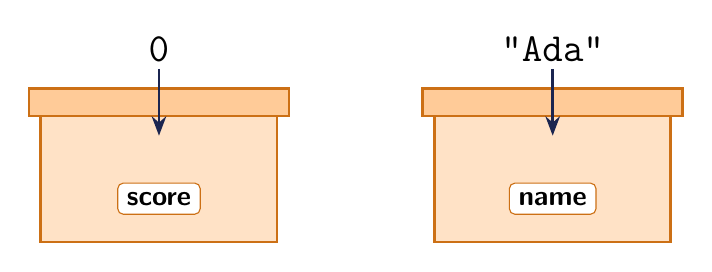
\begin{tikzpicture}[font=\sffamily]
  \foreach \x/\lab/\val in {0/score/0, 5/name/"Ada"}{
    \fill[variables!25] (\x,0) -- (\x+3,0) -- (\x+3,1.6) -- (\x,1.6) -- cycle;
    \draw[variables!80!black, line width=1pt] (\x,0) rectangle (\x+3,1.6);
    \draw[variables!80!black, line width=1pt, fill=variables!45] (\x-0.15,1.6) -- (\x+3.15,1.6) -- (\x+3.15,1.95) -- (\x-0.15,1.95) -- cycle;
    \node[fill=white, draw=variables!80!black, rounded corners=2pt, font=\sffamily\bfseries] at (\x+1.5,0.55) {\lab};
    \node[font=\ttfamily\Large] at (\x+1.5,2.45) {\val};
    \draw[-{Stealth[length=7pt]}, line width=1pt, ink] (\x+1.5,2.2) -- (\x+1.5,1.35);
  }
\end{tikzpicture}
\end{center}

\textbf{How it works:} \py|score = 0| means ``put 0 in the box labelled \texttt{score}''. In Python, one \texttt{=} does \textbf{not} mean ``equals''. It means \textbf{put in the box}. Read it from right to left: the value on the right goes into the box on the left. A box holds one thing at a time, so putting something new in throws the old thing out.

\begin{think}[Why does \texttt{"Ada"} have quote marks?]
Quote marks tell Python ``this is writing''. Without them, \py|name = Ada| makes Python look for a box called \texttt{Ada}, and it can't find one. Numbers like \texttt{0} don't need quote marks.
\end{think}

% ---------------------------------------------------------------------
\needspace{12\baselineskip}
\subsection*{Change the score}

\begin{tcbraster}[raster columns=2, raster equal height=rows, raster column skip=12pt, raster valign=center]
\begin{tcolorbox}[colback=white, colframe=white, boxrule=0pt, valign=center]
\begin{scratch}
\blockvariable{set \selectmenu{score} to \ovalnum{0}}
\blockvariable{change \selectmenu{score} by \ovalnum{1}}
\blockvariable{change \selectmenu{score} by \ovalnum{1}}
\end{scratch}
\end{tcolorbox}
\begin{code}
score = 0
score = score + 1
score += 1
\end{code}
\end{tcbraster}

\textbf{How it works:} Line 2 looks strange if you think \texttt{=} means ``equals''. But remember, it means \textbf{put in the box}. Python works out the right side first: ``what's in \texttt{score}, plus 1''. That is 1. Then it puts the 1 back in the box. Line 3 is a shortcut that does exactly the same thing: \py|score += 1| means ``change score by 1''. After both lines, \texttt{score} holds 2.

\begin{think}[Going down]
\chip[variables]{change score by -1} is \py|score -= 1| (or \py|score = score - 1|). You can use \texttt{+=}, \texttt{-=}, \texttt{*=} and \texttt{/=}.
\end{think}

% ---------------------------------------------------------------------
\needspace{12\baselineskip}
\subsection*{Show the variable}

In Scratch, ticking the box next to a variable shows a \textbf{monitor} on the stage that updates all by itself. Python has no monitor. Instead, you \texttt{print} the box whenever you want to look inside.

\begin{tcbraster}[raster columns=2, raster equal height=rows, raster column skip=12pt, raster valign=center]
\begin{tcolorbox}[colback=white, colframe=white, boxrule=0pt, valign=center]
\begin{scratch}
\blockvariable{set \selectmenu{score} to \ovalnum{7}}
\blockvariable{show variable \selectmenu{score}}
\blocklook{say \ovaloperator{join \ovalnum{Score: } \ovalvariable{score}}}
\end{scratch}
\end{tcolorbox}
\begin{code}
score = 7
print(score)
print("Score:", score)
\end{code}
\end{tcbraster}

\begin{outputbox}
7\\
Score: 7
\end{outputbox}

\textbf{How it works:} \py|print(score)| has no quote marks around \texttt{score}, so Python shows what is \textbf{inside} the box, not the word ``score''. In line 3, the comma lets you print two things in a row, and Python puts a space between them for you. That is easier than Scratch's \chip[operators]{join} block!

% ---------------------------------------------------------------------
\needspace{12\baselineskip}
\subsection*{Naming your boxes}

Scratch lets you call a variable almost anything, even \texttt{my score} with a space. Python is pickier. A Python name must follow these rules:

\begin{itemize}
  \item \textbf{No spaces.} Use an underscore \texttt{\_} instead: \texttt{my\_score}.
  \item \textbf{Don't start with a digit.} \texttt{score2} is fine, \texttt{2score} is not.
  \item \textbf{Capitals matter.} \texttt{Score} and \texttt{score} are two different boxes.
  \item \textbf{Not a Python word.} You can't call a box \texttt{for} or \texttt{import}, because Python already uses those words.
\end{itemize}

\begin{center}
\renewcommand{\arraystretch}{1.35}
\begin{tabular}{P{3.6cm} P{1.6cm} P{8.4cm}}
\toprule
\textbf{Name} & \textbf{OK?} & \textbf{Why} \\
\midrule
\texttt{score} & \textcolor{chalframe}{\textbf{Yes}} & Small letters are perfect. \\
\texttt{my\_score} & \textcolor{chalframe}{\textbf{Yes}} & The underscore joins the words. \\
\texttt{score2} & \textcolor{chalframe}{\textbf{Yes}} & Digits are fine after the first letter. \\
\texttt{my score} & \textcolor{errframe}{\textbf{No}} & A space. Python thinks these are two names. \\
\texttt{2score} & \textcolor{errframe}{\textbf{No}} & It starts with a digit. \\
\texttt{for} & \textcolor{errframe}{\textbf{No}} & Python already uses this word for loops. \\
\bottomrule
\end{tabular}
\end{center}

\needspace{12\baselineskip}
\begin{watchout}[Watch out: capitals make a different box]
\begin{codenonum}
Score = 10
print(score)
\end{codenonum}
\begin{errorbox}
NameError: name 'score' is not defined
\end{errorbox}
Python only knows the boxes you have made. Read the last line of the red error: it names the box Python can't find. Look closely: the box you made is \texttt{Score}, with a capital S. Use small letters for your names and you will rarely hit this bug.
\end{watchout}

\needspace{10\baselineskip}
\begin{challenge}[Quick quiz: box or bust?]
Tick the names Python will accept. (Answers at the back.)\par
\begin{tabular}{@{}p{4.6cm}p{4.6cm}p{4.6cm}@{}}
\tick \texttt{lives} & \tick \texttt{high score} & \tick \texttt{player\_1} \\
\tick \texttt{1st\_place} & \tick \texttt{bestTime} & \tick \texttt{import} \\
\end{tabular}
\end{challenge}

% ---------------------------------------------------------------------
\needspace{12\baselineskip}
\subsection*{Text or number? Quotes matter!}

Scratch quietly guesses whether something is a number or writing. Python never guesses. \texttt{5} is a number. \texttt{"5"} in quote marks is writing (Python calls writing a \textbf{string}).

\begin{tcbraster}[raster columns=2, raster equal height=rows, raster column skip=12pt, raster valign=center]
\begin{code}
print(5 + 5)
print("5" + "5")
\end{code}
\begin{outputbox}
10\\
55
\end{outputbox}
\end{tcbraster}

\textbf{How it works:} Adding two numbers does maths: 10. Adding two strings sticks them together, like the \chip[operators]{join} block: \texttt{55}. In Scratch, both would give 10. And if you try to add a string and a number, Python stops and complains:

\begin{codenonum}
score = 5
print("Score: " + score)
\end{codenonum}
\begin{errorbox}
TypeError: can only concatenate str (not "int") to str
\end{errorbox}

This means ``I can only join writing to writing, and you gave me a number''. The easy fix is the comma you already know: \py|print("Score:", score)|.

% ---------------------------------------------------------------------
\needspace{8\baselineskip}
\begin{think}[For this sprite only, or for all sprites?]
When you make a Scratch variable, Scratch asks: \textbf{For all sprites} or \textbf{For this sprite only}? In this part, all your Python boxes are like ``for all sprites'': any line in your program can use them. In a later part you will learn how to give each sprite its own boxes, like a cat with its own \texttt{health} and a dog with its own \texttt{health}.
\end{think}

% ---------------------------------------------------------------------
\needspace{12\baselineskip}
\subsection*{Variables can draw too}

A box can hold the size of a shape. Change the box, and every line that uses it changes too.

\noindent\begin{minipage}[t]{0.33\linewidth}\vspace{0pt}
\setscratch{scale=0.85}
\begin{scratch}
\blockinit{when \greenflag clicked}
\blockpen{pen down}
\blockvariable{set \selectmenu{size} to \ovalnum{50}}
\blockrepeat{repeat \ovalnum{4}}{
  \blockmove{move \ovalvariable{size} steps}
  \blockmove{turn \turnright{} \ovalnum{90} degrees}
}
\blockvariable{change \selectmenu{size} by \ovalnum{50}}
\blockrepeat{repeat \ovalnum{4}}{
  \blockmove{move \ovalvariable{size} steps}
  \blockmove{turn \turnright{} \ovalnum{90} degrees}
}
\end{scratch}
\end{minipage}\hfill\begin{minipage}[t]{0.66\linewidth}\vspace{0pt}
\begin{code}
from ColabTurtlePlus.Turtle import *
clearscreen()
initializeTurtle((480, 360))
size = 50
for i in range(4):
    forward(size)
    right(90)
size = size + 50
for i in range(4):
    forward(size)
    right(90)
\end{code}
\end{minipage}

\textbf{How it works:} \py|forward(size)| has no quote marks, so the turtle walks however many steps are in the \texttt{size} box. The first square uses 50. Line 8 makes the box hold 100, so the second square is twice as big. Both squares start from the same corner.

What if you put \py|size = size + 50| \textbf{inside} the loop, so the size grows after every line? You will find out in the \textbf{Growing spiral} mission\ldots

% ---------------------------------------------------------------------
\needspace{8\baselineskip}
\subsection*{A list is a backpack}

A variable holds one thing. A \textbf{list} holds lots of things, in order, under one name. In Scratch you click \textbf{Make a List}. In Python you write square brackets.

\begin{tcbraster}[raster columns=2, raster equal height=rows, raster column skip=12pt, raster valign=center]
\begin{tcolorbox}[colback=white, colframe=white, boxrule=0pt, valign=center, halign=center]
\tcbox[on line, colback=white, colframe=muted, arc=4pt, boxrule=0.8pt]{\sffamily\small Make a List}
\par\medskip
New list name: \textbf{backpack}
\end{tcolorbox}
\begin{code}
backpack = []
print(backpack)
\end{code}
\end{tcbraster}

\textbf{How it works:} The square brackets \texttt{[ ]} are the backpack. With nothing between them, the backpack is empty, and \py|print(backpack)| shows \texttt{[]}. Printing a list is Python's \chip[lists]{show list backpack}.

% ---------------------------------------------------------------------
\needspace{12\baselineskip}
\subsection*{Put things in the backpack}

\begin{tcbraster}[raster columns=2, raster equal height=rows, raster column skip=12pt, raster valign=center]
\begin{tcolorbox}[colback=white, colframe=white, boxrule=0pt, valign=center]
\begin{scratch}
\blocklist{delete all of \selectmenu{backpack}}
\blocklist{add \ovalnum{apple} to \selectmenu{backpack}}
\blocklist{add \ovalnum{torch} to \selectmenu{backpack}}
\blocklist{add \ovalnum{map} to \selectmenu{backpack}}
\end{scratch}
\end{tcolorbox}
\begin{code}
backpack = []
backpack.append("apple")
backpack.append("torch")
backpack.append("map")
print(backpack)
\end{code}
\end{tcbraster}

\begin{outputbox}
{[}'apple', 'torch', 'map']
\end{outputbox}

\textbf{How it works:} \py|append| means ``add to the end''. The dot joins the list's name to the job you want it to do: \py|backpack.append("torch")| means ``backpack, add torch to your end''. You can also fill a backpack in one go: \py|backpack = ["apple", "torch", "map"]|. Commas go between the items.

% ---------------------------------------------------------------------
\needspace{12\baselineskip}
\subsection*{Python counts from 0!}

Think of a list as a train. Each carriage carries one item. Scratch numbers the carriages like seats: 1, 2, 3. Python counts \textbf{how many carriages away from the front} each one is, so the first carriage is number \textbf{0}.

\begin{center}
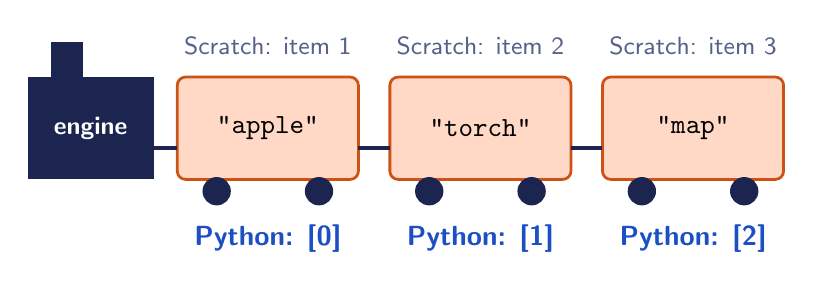
\begin{tikzpicture}[font=\sffamily]
  \fill[ink] (-1.9,0) rectangle (-0.3,1.3);
  \fill[ink] (-1.6,1.3) rectangle (-1.2,1.75);
  \node[white, font=\sffamily\small\bfseries] at (-1.1,0.65) {engine};
  \foreach \i/\item in {0/apple, 1/torch, 2/map}{
    \draw[lists!80!black, line width=1pt, fill=lists!25, rounded corners=3pt] (\i*2.7,0) rectangle (\i*2.7+2.3,1.3);
    \node[font=\ttfamily] at (\i*2.7+1.15,0.65) {"\item"};
    \fill[ink] (\i*2.7+0.5,-0.15) circle (0.18);
    \fill[ink] (\i*2.7+1.8,-0.15) circle (0.18);
    \node[font=\sffamily\small, text=muted] at (\i*2.7+1.15,1.7) {Scratch: item \the\numexpr\i+1\relax};
    \node[font=\sffamily\bfseries, text=kw] at (\i*2.7+1.15,-0.75) {Python: [\i]};
  }
  \draw[ink, line width=1.5pt] (-0.3,0.4) -- (0,0.4);
  \draw[ink, line width=1.5pt] (2.3,0.4) -- (2.7,0.4);
  \draw[ink, line width=1.5pt] (5.0,0.4) -- (5.4,0.4);
\end{tikzpicture}
\end{center}

\begin{tcbraster}[raster columns=2, raster equal height=rows, raster column skip=12pt, raster valign=center]
\begin{tcolorbox}[colback=white, colframe=white, boxrule=0pt, valign=center]
\begin{scratch}
\blocklook{say \ovallist{item \ovalnum{1} of \selectmenu{backpack}}}
\blocklook{say \ovallist{item \ovalnum{3} of \selectmenu{backpack}}}
\end{scratch}
\end{tcolorbox}
\begin{code}
print(backpack[0])
print(backpack[2])
\end{code}
\end{tcbraster}

\begin{outputbox}
apple\\
map
\end{outputbox}

\textbf{How it works:} The square brackets after the name pick one carriage. Here is the rule to remember: \textbf{Scratch item $n$ is Python \texttt{[n - 1]}}. Item 1 is \py|backpack[0]|, item 3 is \py|backpack[2]|.

% ---------------------------------------------------------------------
\needspace{12\baselineskip}
\subsection*{How long is the list?}

\begin{tcbraster}[raster columns=2, raster equal height=rows, raster column skip=12pt, raster valign=center]
\begin{tcolorbox}[colback=white, colframe=white, boxrule=0pt, valign=center]
\begin{scratch}
\blocklook{say \ovallist{length of \selectmenu{backpack}}}
\end{scratch}
\end{tcolorbox}
\begin{code}
print(len(backpack))
\end{code}
\end{tcbraster}

\textbf{How it works:} \py|len| is short for \textbf{length}. It counts the carriages: for our backpack it gives \texttt{3}. Notice that the length is 3 but the last item is \py|backpack[2]|. That is the count-from-0 rule again.

% ---------------------------------------------------------------------
\needspace{12\baselineskip}
\subsection*{Take things out}

\begin{tcbraster}[raster columns=2, raster equal height=rows, raster column skip=12pt, raster valign=center]
\begin{tcolorbox}[colback=white, colframe=white, boxrule=0pt, valign=center]
\begin{scratch}
\blocklist{delete \ovalnum{2} of \selectmenu{backpack}}
\blocklist{delete all of \selectmenu{backpack}}
\end{scratch}
\end{tcolorbox}
\begin{code}
del backpack[1]
backpack.clear()
\end{code}
\end{tcbraster}

\textbf{How it works:} \py|del| is short for \textbf{delete}. Scratch's item 2 is Python's \texttt{[1]}, so \py|del backpack[1]| takes out \texttt{"torch"}, and the train closes the gap: \texttt{['apple', 'map']}. \py|backpack.clear()| empties the whole backpack, leaving \texttt{[]}.

% ---------------------------------------------------------------------
\needspace{12\baselineskip}
\subsection*{Squeeze in and swap}

Start again with \py|backpack = ["apple", "torch", "map"]|.

\begin{center}
\begin{scratch}
\blocklist{insert \ovalnum{rope} at \ovalnum{2} of \selectmenu{backpack}}
\blocklist{replace item \ovalnum{4} of \selectmenu{backpack} with \ovalnum{lamp}}
\end{scratch}
\end{center}
\begin{code}
backpack.insert(1, "rope")
backpack[3] = "lamp"
\end{code}

\begin{outputbox}[After line 1, then after line 2]
{[}'apple', 'rope', 'torch', 'map']\\
{[}'apple', 'rope', 'torch', 'lamp']
\end{outputbox}

\textbf{How it works:} \py|insert(1, "rope")| squeezes a new carriage in at place 1 (Scratch's place 2), and the others shuffle back. \py|backpack[3] = "lamp"| uses the ``put in the box'' sign: carriage 3 (Scratch's item 4) gets a new item, and the old \texttt{"map"} is thrown out. Each carriage works like a little box!

% ---------------------------------------------------------------------
\needspace{12\baselineskip}
\subsection*{Is it in the backpack?}

\begin{center}
\begin{scratch}
\blocklook{say \boollist{\selectmenu{backpack} contains \ovalnum{torch} ?}}
\blocklook{say \boollist{\selectmenu{backpack} contains \ovalnum{sword} ?}}
\end{scratch}
\end{center}
\begin{code}
backpack = ["apple", "torch", "map"]
print("torch" in backpack)
print("sword" in backpack)
\end{code}

\begin{outputbox}
True\\
False
\end{outputbox}

\textbf{How it works:} \py|"sword" in backpack| asks a yes-or-no question. Python answers \texttt{True} (yes) or \texttt{False} (no), where Scratch says \texttt{true} or \texttt{false}. In Part 5 you will use questions like this with \py|if|, to do something only when the sword is there.

\begin{watchout}[Watch out: capitals again]
Scratch thinks \texttt{Torch} and \texttt{torch} are the same. Python doesn't: \py|"Torch" in backpack| is \texttt{False}. Type your items exactly.
\end{watchout}

% ---------------------------------------------------------------------
\needspace{24\baselineskip}
\subsection*{A Python power: walk through the backpack}

In Scratch, to visit every item you need a counter variable, \chip[control]{repeat (length of backpack)} and \chip[lists]{item (i) of backpack}. Python has a much shorter way.

\begin{center}
\begin{scratch}
\blockvariable{set \selectmenu{i} to \ovalnum{1}}
\blockrepeat{repeat \ovallist{length of \selectmenu{backpack}}}{
  \blocklook{say \ovallist{item \ovalvariable{i} of \selectmenu{backpack}} for \ovalnum{1} seconds}
  \blockvariable{change \selectmenu{i} by \ovalnum{1}}
}
\end{scratch}
\end{center}
\begin{code}
for thing in backpack:
    print("In my backpack:", thing)
\end{code}

\begin{outputbox}
In my backpack: apple\\
In my backpack: torch\\
In my backpack: map
\end{outputbox}

\textbf{How it works:} \py|for thing in backpack:| means ``take each item out of the backpack in turn, and call it \texttt{thing}''. The first time round the loop, \texttt{thing} holds \texttt{"apple"}, then \texttt{"torch"}, then \texttt{"map"}. You get to choose the name: \py|for snack in snacks:| reads nicely. No counter, no \texttt{- 1}, no mistakes!

% ---------------------------------------------------------------------
\needspace{12\baselineskip}
\subsection*{Pick one at random}

\begin{center}
\begin{scratch}
\blocklook{say \ovallist{item \ovalnum{random} of \selectmenu{snacks}}}
\end{scratch}
\end{center}
\begin{code}
import random
snacks = ["crisps", "banana", "cookie"]
print(random.choice(snacks))
\end{code}

\textbf{How it works:} Did you know you can type \texttt{random} into Scratch's \chip[lists]{item 1 of} block? Python's version is \py|random.choice(snacks)|: it reaches into the list without looking and pulls out one item. Like \py|import time| in Part 2, \py|import random| brings in Python's random tools first. Run it a few times: you won't always get the same snack.

% ---------------------------------------------------------------------
\needspace{12\baselineskip}
\begin{watchout}[Watch out: Python tells you when a carriage is missing]
Ask Scratch for \chip[lists]{item 4 of backpack} when there are only 3 items, and Scratch quietly gives you nothing. Python stops and tells you:
\begin{codenonum}
backpack = ["apple", "torch", "map"]
print(backpack[3])
\end{codenonum}
\begin{errorbox}
IndexError: list index out of range
\end{errorbox}
\textbf{Index} is Python's word for a carriage number. ``Out of range'' means ``there is no carriage with that number''. A list of 3 has carriages 0, 1 and 2 only. This error is a clue note, not a telling-off: it shows you exactly which line to fix.
\end{watchout}

% =====================================================================
\mission{Score counter}{making a variable, changing it in a loop, and printing it}

Every game needs a score. This program gives you 10 points every second, five times, and shows the score each time, just like a Scratch monitor ticking up.

\step{Step 1: Build it in Scratch}
\noindent\begin{minipage}[t]{0.52\linewidth}\vspace{0pt}
\begin{scratch}
\blockinit{when \greenflag clicked}
\blockvariable{set \selectmenu{score} to \ovalnum{0}}
\blockvariable{show variable \selectmenu{score}}
\blockrepeat{repeat \ovalnum{5}}{
  \blockcontrol{wait \ovalnum{1} seconds}
  \blockvariable{change \selectmenu{score} by \ovalnum{10}}
}
\blocklook{say \ovaloperator{join \ovalnum{Game over! Final score: } \ovalvariable{score}}}
\end{scratch}
\end{minipage}\hfill\begin{minipage}[t]{0.39\linewidth}\vspace{0pt}
Click \textbf{Make a Variable} and call it \textbf{score}. Then build:
\end{minipage}


\step{Step 2: Type it in Colab}
This one doesn't draw, so you don't need the three starting lines.

\begin{typethis}
import time
score = 0
print("Score:", score)
for i in range(5):
    time.sleep(1)
    score = score + 10
    print("Score:", score)
print("Game over! Final score:", score)
\end{typethis}

\needspace{8\baselineskip}
\step{Step 3: Read it line by line}

\begin{longtable}{>{\centering\arraybackslash}p{1.1cm} P{5.3cm} P{9.1cm}}
\toprule
\textbf{Line} & \textbf{Scratch block} & \textbf{What it means} \\
\midrule
--- & \chip[events]{when green flag clicked} & No code needed. The play button \playbtn{} starts it. \\
1 & (wait needs this) & Brings in Python's clock tools, so we can use \py|time.sleep|. \\
2 & \chip[variables]{set score to 0} & Makes a box called \texttt{score} and puts 0 in it. \\
3 & \chip[variables]{show variable score} & Shows what is in the box: \texttt{Score: 0}. \\
4 & \chip[control]{repeat 5} & Do the indented lines 5 times. \\
5 & \chip[control]{wait 1 seconds} & Wait one second. \\
6 & \chip[variables]{change score by 10} & Take what's in the box, add 10, and put it back. \\
7 & (the monitor updates) & Scratch's monitor changes by itself. In Python, we print again to see the new score. \\
8 & \chip[looks]{say join Game over! \ldots} & No spaces in front, so it runs once, after the loop. \\
\bottomrule
\end{longtable}

\step{Step 4: Run it}
Press \playbtn. A new line appears every second.

\noindent\begin{minipage}[t]{0.36\linewidth}\vspace{0pt}
\begin{outputbox}
Score: 0\\
Score: 10\\
Score: 20\\
Score: 30\\
Score: 40\\
Score: 50\\
Game over! Final score: 50
\end{outputbox}
\end{minipage}\hfill\begin{minipage}[t]{0.55\linewidth}\vspace{0pt}
\begin{think}[What if you forget line 2?]
Delete line 2 and click \textbf{Runtime}, then \textbf{Restart session}, then run the cell again. Python says \texttt{NameError: name 'score' is not defined}. You can't add 10 to a box that doesn't exist yet! In Scratch, a new variable starts at 0 by itself. In Python, you always fill the box first.
\end{think}
\end{minipage}


\begin{challenge}
\tick Change line 6 to \py|score += 10|. Does anything change when you run it?\par
\tick Make it count \textbf{down}: start the score at 50 and take away 10 each time. (Hint: \texttt{-=}.)\par
\tick Add a second box, \py|lives = 3|, before the loop. Inside the loop, take one life away and print both: \py|print("Score:", score, "Lives:", lives)|. What happens to the lives after 5 goes?\par
\tick \textbf{Super challenge:} make the points get bigger each time. Add \py|points = 10| before the loop. Inside it, add \py|points| to the score, then make \py|points| 10 bigger. What is the final score?
\end{challenge}

% =====================================================================
\mission{Growing spiral}{using a variable for the size, and changing it inside a loop}

On the ``Variables can draw too'' page, the size changed once, between two squares. Now the size grows a little after \textbf{every} line. Each line is longer than the one before, and the turtle spirals outwards.

\step{Step 1 and Step 2: Build it in Scratch, then type it in Colab}
Make a variable called \textbf{size}. Add the \textbf{Pen} extension, then build the script on the left. Then type the Python on the right.

\noindent\begin{minipage}[t]{0.33\linewidth}\vspace{0pt}
\setscratch{scale=0.85}
\begin{scratch}
\blockinit{when \greenflag clicked}
\blockpen{erase all}
\blockpen{pen down}
\blockpen{set pen color to \ovalnum{purple}}
\blockvariable{set \selectmenu{size} to \ovalnum{5}}
\blockrepeat{repeat \ovalnum{40}}{
  \blockmove{move \ovalvariable{size} steps}
  \blockmove{turn \turnright{} \ovalnum{90} degrees}
  \blockvariable{change \selectmenu{size} by \ovalnum{5}}
}
\end{scratch}
\end{minipage}\hfill\begin{minipage}[t]{0.66\linewidth}\vspace{0pt}
\begin{typethis}
from ColabTurtlePlus.Turtle import *
clearscreen()
initializeTurtle((480, 360))
speed(13)
pencolor("purple")
size = 5
for i in range(40):
    forward(size)
    right(90)
    size = size + 5
\end{typethis}
\end{minipage}

\step{Step 3: Read it line by line}

\begin{longtable}{>{\centering\arraybackslash}p{1.1cm} P{5.3cm} P{9.1cm}}
\toprule
\textbf{Line} & \textbf{Scratch block} & \textbf{What it means} \\
\midrule
1--3 & \chip[events]{when green flag clicked}\newline\chip[pen]{erase all} & The three starting lines. \py|clearscreen()| wipes the stage, like \chip[pen]{erase all}. The pen starts down. \\
4 & & The fastest speed, so you don't wait too long. \\
5 & \chip[pen]{set pen color to purple} & Colour names go in quote marks, in small letters. \\
6 & \chip[variables]{set size to 5} & The first line will be 5 steps long. \\
7 & \chip[control]{repeat 40} & Do the indented lines 40 times. \\
8 & \chip[motion]{move (size) steps} & Walk forward by whatever is in the \texttt{size} box right now. \\
9 & \chip[motion]{turn right 90 degrees} & Turn a corner. \\
10 & \chip[variables]{change size by 5} & Make the box 5 bigger, \textbf{inside} the loop, so the next line is longer. \\
\bottomrule
\end{longtable}

\step{Step 4: Run it}
A purple square spiral grows out from the middle of the stage. The lines go 5, 10, 15, 20 \ldots{} steps, and the last one is 200 steps long.

\begin{think}[Spaces matter]
Line 10 has four spaces in front, so it is inside the loop. Take the spaces away and run it. Now \py|size| only changes \textbf{once}, after the loop has finished, so every line is 5 steps long and the turtle just goes round a tiny square 40 times. No red error, but the wrong drawing!
\end{think}

\begin{challenge}
\tick Change \py|right(90)| to \py|right(91)|. The spiral twists! Try 89, 120 and 144 too.\par
\tick Make the spiral tighter with \py|size = size + 2|, or looser with \py|size = size + 8|. With \texttt{+ 8}, does it still fit on the stage?\par
\tick Make the pen thicker as well: add \py|thick = 1| before the loop, then \py|pensize(thick)| and \py|thick = thick + 0.2| inside it.\par
\tick \textbf{Super challenge:} make a spiral that \textbf{shrinks}. Start at \py|size = 200| and take away 5 each time. (Hint: so it fits on the stage, jump to \py|goto(-100, 100)| with the pen up before you start.)
\end{challenge}

% =====================================================================
\mission{Rainbow from a colour list}{a list of colours, and a \texttt{for} loop that walks through it}

A rainbow is a list of colours! This program keeps the six colours in a list, then draws one thick stripe for each colour, from top to bottom.

\step{Step 1: Build it in Scratch}
\noindent\begin{minipage}[t]{0.61\linewidth}\vspace{0pt}
\begin{scratch}
\blockinit{when \greenflag clicked}
\blockpen{erase all}
\blockpen{set pen size to \ovalnum{15}}
\blockvariable{set \selectmenu{y} to \ovalnum{60}}
\blockvariable{set \selectmenu{i} to \ovalnum{1}}
\blockrepeat{repeat \ovallist{length of \selectmenu{colours}}}{
  \blockpen{set pen color to \ovallist{item \ovalvariable{i} of \selectmenu{colours}}}
  \blockpen{pen up}
  \blockmove{go to x: \ovalnum{-150} y: \ovalvariable{y}}
  \blockpen{pen down}
  \blockmove{move \ovalnum{300} steps}
  \blockvariable{change \selectmenu{y} by \ovalnum{-15}}
  \blockvariable{change \selectmenu{i} by \ovalnum{1}}
}
\end{scratch}
\end{minipage}\hfill\begin{minipage}[t]{0.36\linewidth}\vspace{0pt}
Make a list called \textbf{colours} and two variables called \textbf{y} and \textbf{i}. Scratch's pen doesn't understand colour names, so fill the list on the stage with six colour codes: \texttt{\#FF0000}, \texttt{\#FFA500}, \texttt{\#FFFF00}, \texttt{\#008000}, \texttt{\#0000FF}, \texttt{\#800080}. Then build:
\end{minipage}


\step{Step 2: Type it in Colab}

\begin{typethis}
from ColabTurtlePlus.Turtle import *
clearscreen()
initializeTurtle((480, 360))
speed(13)
pensize(15)
colours = ["red", "orange", "yellow",
           "green", "blue", "purple"]
y = 60
for colour in colours:
    pencolor(colour)
    penup()
    goto(-150, y)
    pendown()
    forward(300)
    y = y - 15
hideturtle()
\end{typethis}

\par\medskip{\large\bfseries\color{ink}Step 3: Read it line by line}\par\nopagebreak

\begin{longtable}{>{\centering\arraybackslash}p{1.1cm} P{5.3cm} P{9.1cm}}
\toprule
\textbf{Line} & \textbf{Scratch block} & \textbf{What it means} \\
\midrule
1--3 & \chip[events]{when green flag clicked} & The three starting lines. They also do \chip[pen]{erase all}. \\
4--5 & \chip[pen]{set pen size to 15} & The fastest speed, and thick stripes. \\
6--7 & (the list on the stage) & Six colour names. Inside square brackets you may carry on to the next line. \\
8 & \chip[variables]{set y to 60} & The first stripe is at $y = 60$. \\
9 & \chip[control]{repeat length of colours} & Take out each colour in turn, and call it \texttt{colour}. No counter \texttt{i}! \\
10 & \chip[pen]{set pen color to}\newline\chip[lists]{item i of colours} & Use the colour we just took out. \texttt{colour} has no quote marks: it is a box, not the word ``colour''. Python understands colour \textbf{names}, so no codes are needed. \\
11--13 & \chip[pen]{pen up}\newline\chip[motion]{go to x: -150 y: (y)}\newline\chip[pen]{pen down} & Jump to the left end of this stripe without drawing. \\
14 & \chip[motion]{move 300 steps} & Draw the stripe. The turtle faces right. \\
15 & \chip[variables]{change y by -15} & Move down 15 for the next stripe. Then line 16 hides the turtle. \\
\bottomrule
\end{longtable}

\step{Step 4: Run it}
Six thick stripes appear one under another: red at the top, then orange, yellow, green, blue and purple at the bottom.

\begin{think}[Colour and \texttt{colour}]
In this book we spell it \textbf{colour}. Python was written in America, so its own words use \textbf{color}: \py|pencolor|. Our list and box names can use any spelling we like, as long as we always spell them the same way.
\end{think}

\begin{challenge}
\tick Add a seventh stripe with \py|colours.append("pink")| on a new line after line 7.\par
\tick Leave gaps between the stripes: change \texttt{15} in line 15 to \texttt{20}.\par
\tick Make your own flag. Change the list to \py|["red", "white", "blue"]|. Which countries could you make?\par
\tick \textbf{Super challenge:} make every stripe shorter than the one above it. Add \py|length = 300| before the loop, use \py|forward(length)|, and take 30 off \texttt{length} each time round.
\end{challenge}

% =====================================================================
\mission{Random story maker}{filling lists, adding to them, and picking with \texttt{random.choice}}

Three lists, one pinch of randomness, and you get a silly sentence every time. Will a dragon eat your homework?

\step{Step 1: Build it in Scratch}
\noindent\begin{minipage}[t]{0.68\linewidth}\vspace{0pt}
\begin{scratch}
\blockinit{when \greenflag clicked}
\blocklist{add \ovalnum{my homework} to \selectmenu{things}}
\blockrepeat{repeat \ovalnum{3}}{
  \blockvariable{set \selectmenu{hero} to \ovallist{item \ovalnum{random} of \selectmenu{heroes}}}
  \blockvariable{set \selectmenu{action} to \ovallist{item \ovalnum{random} of \selectmenu{actions}}}
  \blockvariable{set \selectmenu{thing} to \ovallist{item \ovalnum{random} of \selectmenu{things}}}
  \blocklook{say \ovaloperator{join \ovalvariable{hero} \ovaloperator{join \ovalvariable{action} \ovalvariable{thing}}} for \ovalnum{2} seconds}
}
\end{scratch}
\end{minipage}\hfill\begin{minipage}[t]{0.29\linewidth}\vspace{0pt}
Make three lists, \textbf{heroes}, \textbf{actions} and \textbf{things}, and fill them on the stage. Make three variables, \textbf{hero}, \textbf{action} and \textbf{thing}. Then build:
\end{minipage}


\step{Step 2: Type it in Colab}

\begin{typethis}
import random
heroes = ["A dragon", "My teacher", "A tiny robot"]
actions = ["ate", "sang to", "tickled"]
things = ["a banana", "the moon", "a sock"]
things.append("my homework")
for i in range(3):
    hero = random.choice(heroes)
    action = random.choice(actions)
    thing = random.choice(things)
    print(hero, action, thing)
\end{typethis}

\needspace{8\baselineskip}
\step{Step 3: Read it line by line}

\begin{longtable}{>{\centering\arraybackslash}p{1.1cm} P{5.3cm} P{9.1cm}}
\toprule
\textbf{Line} & \textbf{Scratch block} & \textbf{What it means} \\
\midrule
1 & & Brings in Python's random tools. \\
2--4 & (lists filled on the stage) & Three lists, each with three items. Each item is a string, so each has quote marks. Commas go between items. \\
5 & \chip[lists]{add my homework to things} & Puts a fourth thing on the end of the \texttt{things} list. \\
6 & \chip[control]{repeat 3} & Make three sentences. \\
7--9 & \chip[variables]{set hero to}\newline\chip[lists]{item random of heroes} \ldots & Pick one item from each list, and put it in a box. \\
10 & \chip[looks]{say join hero \ldots} & Print the three boxes in a row. The commas put spaces between them, so you don't need three \chip[operators]{join} blocks. \\
\bottomrule
\end{longtable}

\step{Step 4: Run it}
You will get three random sentences. Yours will be different!

\begin{outputbox}[You might see]
A dragon ate a sock\\
A tiny robot tickled my homework\\
My teacher sang to the moon
\end{outputbox}

\begin{think}[Click the flag twice]
In Scratch, lists remember their items even after the project stops. Click the green flag twice, and \texttt{my homework} is added \textbf{twice}! In Python, line 4 makes a fresh \texttt{things} list every time you run the cell, so it always starts with exactly three things.
\end{think}

\begin{challenge}
\tick Add your own words to each list. Don't forget the quote marks and commas!\par
\tick Make 5 sentences instead of 3.\par
\tick Add a fourth list, \texttt{places}, like \py|["in the bath", "on the bus"]|, and print a place at the end of each sentence.\par
\tick \textbf{Super challenge:} after the loop, print \py|len(things)| and the whole \texttt{things} list. How many things are there, and where did \texttt{"my homework"} go?
\end{challenge}

% =====================================================================
\banner{variables}{YOUR TURN}{Translate it yourself}

You are the translator now! Write the Python for this new Scratch script, then run it in Colab.

\noindent\begin{minipage}[t]{0.47\linewidth}\vspace{0pt}
\setscratch{scale=0.9}
\begin{scratch}
\blockinit{when \greenflag clicked}
\blocklist{delete all of \selectmenu{pets}}
\blocklist{add \ovalnum{cat} to \selectmenu{pets}}
\blocklist{add \ovalnum{dog} to \selectmenu{pets}}
\blocklist{add \ovalnum{fish} to \selectmenu{pets}}
\blocklook{say \ovallist{length of \selectmenu{pets}} for \ovalnum{2} seconds}
\blocklook{say \ovallist{item \ovalnum{2} of \selectmenu{pets}} for \ovalnum{2} seconds}
\end{scratch}
\end{minipage}\hfill\begin{minipage}[t]{0.5\linewidth}\vspace{0pt}
\begin{tcolorbox}[colback=white, colframe=codeframe, arc=5pt, title=\textbf{My Python}, coltitle=ink, colbacktitle=codebg]
\vspace{4pt}
\foreach \n in {1,...,6}{\rule{\linewidth}{0.4pt}\par\vspace{9pt}}
\end{tcolorbox}
\small\textbf{Hints:} What starts an empty list? Which word adds to the end? Item 2 is not \texttt{[2]}!
\end{minipage}

\medskip
\begin{puzzle}
Can you count the items in a list \textbf{without} \py|len|? Write the \textbf{two} missing lines, using a \py|for| loop and \texttt{+=}. It should print \texttt{4}.
\begin{codenonum}
words = ["tiger", "lion", "zebra", "hippo"]
count = 0
\end{codenonum}
\vspace{10pt}
\rule{\linewidth}{0.4pt}\par\vspace{10pt}
\rule{\linewidth}{0.4pt}\par\vspace{2pt}
\hspace*{8pt}\texttt{print(count)}
\end{puzzle}

\smallskip
\begin{tcolorbox}[colback=variables!10, colframe=variables!80!black, arc=6pt, boxrule=0.8pt, left=10pt, top=2pt, bottom=2pt, title={\textbf{Part 3 checklist}}, coltitle=white, colbacktitle=variables!80!black]
\tick I can make a variable with \py|=| and explain that it means ``put in the box''.\par
\tick I can change a variable with \py|score += 1| and show it with \py|print|.\par
\tick I know the naming rules, and that \texttt{5} and \texttt{"5"} are different.\par
\tick I can make a list and use \py|append|, \py|len|, \py|del|, \py|insert| and \py|clear|.\par
\tick I remember that Scratch item 1 is Python \texttt{[0]}, and I know what \texttt{IndexError} means.\par
\tick I can walk through a list with \py|for| and pick at random with \py|random.choice|.
\end{tcolorbox}

% =====================================================================
% PART 4: Operators
% =====================================================================
\partopener{operators}{PART 4}{Operators}{Do maths, roll dice, compare things and take words apart.}
\setscratch{scale=0.8}

The green \textbf{Operators} blocks are the thinking blocks of Scratch. They do sums, pick random numbers, check whether things are true, and play with words. In this part you will meet the Python version of every one of them:

\begin{itemize}
  \item \chip[operators]{7 + 2} becomes \py|7 + 2|
  \item \chip[operators]{pick random 1 to 6} becomes \py|random.randint(1, 6)|
  \item \chip[operators]{join Hello Sam} becomes \py|"Hello " + "Sam"|
  \item \chip[operators]{letter 1 of banana} becomes \py|"banana"[0]|
\end{itemize}

Most of the programs in this part \textbf{don't draw}, so you don't need the three starting lines. Just make a new cell with \textbf{+ Code}, type, and press \playbtn.

\begin{think}[A friendly waiter and a strict robot chef]
Scratch is like a friendly waiter. If you ask for something a bit muddled, it guesses what you meant. Python is like a strict robot chef. It does \textbf{exactly} what you say, and if your order doesn't make sense, it stops and tells you why. That sounds annoying, but it means Python never quietly guesses wrong. Look out for the \textbf{Watch out!} boxes in this part: they show the places where the robot chef is fussier than the waiter.
\end{think}

% ---------------------------------------------------------------------
\needspace{15\baselineskip}
\subsection*{Doing sums: + -- * /}

In Scratch you can drop a green sum block into a \chip[looks]{say} block. In Python you put the sum inside \py|print( )|.

\begin{tcbraster}[raster columns=2, raster equal height=rows, raster column skip=12pt, raster valign=center, raster force size=false, raster odd column/.style={add to width=-1.2cm}, raster even column/.style={add to width=1.2cm}]
\begin{tcolorbox}[colback=white, colframe=white, boxrule=0pt, valign=center]
\begin{scratch}
\blockinit{when \greenflag clicked}
\blocklook{say \ovaloperator{\ovalnum{7} + \ovalnum{2}} for \ovalnum{1} seconds}
\blocklook{say \ovaloperator{\ovalnum{7} - \ovalnum{2}} for \ovalnum{1} seconds}
\blocklook{say \ovaloperator{\ovalnum{7} * \ovalnum{2}} for \ovalnum{1} seconds}
\blocklook{say \ovaloperator{\ovalnum{7} / \ovalnum{2}} for \ovalnum{1} seconds}
\end{scratch}
\end{tcolorbox}
\begin{tcolorbox}[colback=white, colframe=white, boxrule=0pt, left=0pt, right=0pt, top=0pt, bottom=0pt, valign=center]
\begin{code}
print(7 + 2)
print(7 - 2)
print(7 * 2)
print(7 / 2)
\end{code}
\begin{outputbox}
9\\
5\\
14\\
3.5
\end{outputbox}
\end{tcolorbox}
\end{tcbraster}

\textbf{How it works.} The signs are the same as in Scratch: \texttt{*} (a star) means times, and \texttt{/} (a slash) means divide. You don't need the green oval: the numbers and the sign just sit next to each other. Put spaces around the sign so it is easy to read.

\needspace{10\baselineskip}
\begin{watchout}[Watch out: divide always gives a decimal]
In Python, \texttt{/} always gives a number with a decimal point, even when it divides exactly. \py|print(6 / 2)| shows \texttt{3.0}, not \texttt{3}. It is still the right answer!

\textbf{Bonus:} two slashes, \texttt{//}, divide and throw away the leftover part. \py|print(7 // 2)| shows \texttt{3}. Scratch has no block for this.
\end{watchout}

\needspace{14\baselineskip}
\begin{think}[Brackets are the green ovals]
In Scratch, you choose which sum happens first by putting one block \textbf{inside} another. In Python you use brackets. Without brackets, Python does times and divide before plus and minus, just like in maths lessons:
\begin{center}
\begin{tabular}{l@{\hspace{1.5cm}}l}
\ovaloperator{\ovalnum{2} + \ovaloperator{\ovalnum{3} * \ovalnum{4}}} & \py|2 + 3 * 4| gives \texttt{14} \\[8pt]
\ovaloperator{\ovaloperator{\ovalnum{2} + \ovalnum{3}} * \ovalnum{4}} & \py|(2 + 3) * 4| gives \texttt{20}
\end{tabular}
\end{center}
\end{think}

% ---------------------------------------------------------------------
\needspace{15\baselineskip}
\subsection*{Pick random}

\begin{tcbraster}[raster columns=2, raster equal height=rows, raster column skip=12pt, raster valign=center, raster force size=false, raster odd column/.style={add to width=-1.2cm}, raster even column/.style={add to width=1.2cm}]
\begin{tcolorbox}[colback=white, colframe=white, boxrule=0pt, valign=center]
\begin{scratch}
\blockinit{when \greenflag clicked}
\blockvariable{set \selectmenu{roll} to \ovaloperator{pick random \ovalnum{1} to \ovalnum{6}}}
\blocklook{say \ovalvariable{roll}}
\end{scratch}
\end{tcolorbox}
\begin{code}
import random
roll = random.randint(1, 6)
print(roll)
\end{code}
\end{tcbraster}

\textbf{How it works.} \py|import random| is like clicking the \textbf{Extensions} button: it brings in Python's random-number tools. You only need it once, at the top of the cell. \py|random.randint(1, 6)| means ``from the random tools, pick a whole number (an \textbf{int}eger) from 1 to 6''. The dot means ``from inside''. Just like Scratch, \textbf{both ends are included}, so you can get 1 and you can get 6. Run the cell a few times: you get a different number each time.

\begin{watchout}[Watch out: smallest number first]
Scratch doesn't mind \chip[operators]{pick random 6 to 1}: it swaps the numbers for you. Python stops with \texttt{ValueError: empty range}. Always put the smaller number first.
\end{watchout}

% ---------------------------------------------------------------------
\needspace{15\baselineskip}
\subsection*{Bigger, smaller, the same: > < ==}

The pointy green blocks answer a question with \textbf{true} or \textbf{false}. You can drop one into a \chip[looks]{say} block to see the answer. In Python, the answer is \py|True| or \py|False|.

\begin{tcbraster}[raster columns=2, raster equal height=rows, raster column skip=12pt, raster valign=center, raster force size=false, raster odd column/.style={add to width=-1.2cm}, raster even column/.style={add to width=1.2cm}]
\begin{tcolorbox}[colback=white, colframe=white, boxrule=0pt, valign=center]
\begin{scratch}
\blockinit{when \greenflag clicked}
\blockvariable{set \selectmenu{score} to \ovalnum{10}}
\blocklook{say \booloperator{\ovalnum{5} > \ovalnum{3}} for \ovalnum{1} seconds}
\blocklook{say \booloperator{\ovalnum{5} < \ovalnum{3}} for \ovalnum{1} seconds}
\blocklook{say \booloperator{\ovalvariable{score} = \ovalnum{10}}}
\end{scratch}
\end{tcolorbox}
\begin{tcolorbox}[colback=white, colframe=white, boxrule=0pt, left=0pt, right=0pt, top=0pt, bottom=0pt, valign=center]
\begin{code}
score = 10
print(5 > 3)
print(5 < 3)
print(score == 10)
\end{code}
\begin{outputbox}
True\\
False\\
True
\end{outputbox}
\end{tcolorbox}
\end{tcbraster}

\textbf{How it works.} \texttt{>} and \texttt{<} are the same as in Scratch. To check whether two things are the same, Python uses \textbf{two} equals signs, \texttt{==}. Remember from Part 3: \textbf{one} equals sign puts a value in a box (\py|score = 10|). Two equals signs ask a question: ``is \texttt{score} the same as 10?'' \py|True| and \py|False| always start with a capital letter.

In Part 5 you will put these questions inside \py|if|, to make the program decide what to do. For now, we just print the answers.

\begin{think}[Two blocks Scratch doesn't have]
Python can also ask ``bigger \textbf{or the same}'' with \texttt{>=}, and ``smaller or the same'' with \texttt{<=}. \py|print(10 >= 10)| shows \texttt{True}. And \texttt{!=} means ``is \textbf{not} the same as''.
\end{think}

\needspace{12\baselineskip}
\begin{watchout}[Watch out: capital letters count!]
In Scratch, \chip[operators]{Cat = cat} is \textbf{true}. Scratch doesn't care about capital letters. Python does: \py|print("Cat" == "cat")| shows \texttt{False}.

The fix is \py|.lower()|, which turns writing into small letters before you compare:\par
\py|print("Cat".lower() == "cat".lower())| shows \texttt{True}.
\end{watchout}

% ---------------------------------------------------------------------
\needspace{15\baselineskip}
\subsection*{and, or, not}

\begin{tcbraster}[raster columns=2, raster equal height=rows, raster column skip=12pt, raster valign=center, raster force size=false, raster odd column/.style={add to width=-1.2cm}, raster even column/.style={add to width=1.2cm}]
\begin{tcolorbox}[colback=white, colframe=white, boxrule=0pt, valign=center]
\begin{scratch}
\blockinit{when \greenflag clicked}
\blockvariable{set \selectmenu{age} to \ovalnum{9}}
\blocklook{say \booloperator{\booloperator{\ovalvariable{age} > \ovalnum{8}} and \booloperator{\ovalvariable{age} < \ovalnum{12}}}}
\blocklook{say \booloperator{\booloperator{\ovalvariable{age} < \ovalnum{5}} or \booloperator{\ovalvariable{age} > \ovalnum{10}}}}
\blocklook{say \booloperator{not \booloperator{\ovalvariable{age} > \ovalnum{8}}}}
\end{scratch}
\end{tcolorbox}
\begin{tcolorbox}[colback=white, colframe=white, boxrule=0pt, left=0pt, right=0pt, top=0pt, bottom=0pt, valign=center]
\begin{code}
age = 9
print(age > 8 and age < 12)
print(age < 5 or age > 10)
print(not age > 8)
\end{code}
\begin{outputbox}
True\\
False\\
False
\end{outputbox}
\end{tcolorbox}
\end{tcbraster}

\textbf{How it works.} Python uses the same words as Scratch, written in small letters. \py|and| is \py|True| only when \textbf{both} sides are true. \py|or| is \py|True| when \textbf{at least one} side is true. \py|not| flips the answer: true becomes false and false becomes true. You don't need the extra hexagon shapes: Python works out the \texttt{>} and \texttt{<} questions first, then the \py|and|.

% ---------------------------------------------------------------------
\needspace{15\baselineskip}
\subsection*{Join: sticking words together}

\begin{tcbraster}[raster columns=2, raster equal height=rows, raster column skip=12pt, raster valign=center, raster force size=false, raster odd column/.style={add to width=-1.2cm}, raster even column/.style={add to width=1.2cm}]
\begin{tcolorbox}[colback=white, colframe=white, boxrule=0pt, valign=center]
\begin{scratch}
\blockinit{when \greenflag clicked}
\blockvariable{set \selectmenu{name} to \ovalnum{Sam}}
\blockvariable{set \selectmenu{score} to \ovalnum{7}}
\blocklook{say \ovaloperator{join \ovalnum{Hello } \ovalvariable{name}} for \ovalnum{1} seconds}
\blocklook{say \ovaloperator{join \ovalnum{Score: } \ovalvariable{score}}}
\end{scratch}
\end{tcolorbox}
\begin{tcolorbox}[colback=white, colframe=white, boxrule=0pt, left=0pt, right=0pt, top=0pt, bottom=0pt, valign=center]
\begin{code}
name = "Sam"
score = 7
print("Hello " + name)
print("Score: " + str(score))
\end{code}
\begin{outputbox}
Hello Sam\\
Score: 7
\end{outputbox}
\end{tcolorbox}
\end{tcbraster}

\textbf{How it works.} When \texttt{+} has writing on both sides, it joins them, just like \chip[operators]{join}. Python calls a piece of writing a \textbf{string} (think of letters threaded on a string, like beads). Notice the space inside \py|"Hello "|: without it you would get \texttt{HelloSam}.

\needspace{12\baselineskip}
\begin{watchout}[Watch out: you can't join writing and a number]
\py|print("Score: " + score)| stops with this clue:
\begin{errorbox}
TypeError: can only concatenate str (not "int") to str
\end{errorbox}
``Concatenate'' is a long word for join. Python is saying: ``I can only join a string to a string, and you gave me a number.'' Scratch would just guess. In Python, turn the number into a string first with \py|str(score)|, like line 4 above.
\end{watchout}

\needspace{10\baselineskip}
\begin{think}[Bonus: f-strings, the easy way to join]
Put an \texttt{f} in front of the quote marks, and anything inside curly brackets \texttt{\{ \}} is filled in for you, numbers too:\par
\py|print(f"Score: {score}")| shows \texttt{Score: 7}. No \py|str( )| and no \texttt{+} needed!

And one more trick: \py|print("ha" * 3)| shows \texttt{hahaha}.
\end{think}

% ---------------------------------------------------------------------
\needspace{15\baselineskip}
\subsection*{Letter of, and length of}

\begin{tcbraster}[raster columns=2, raster equal height=rows, raster column skip=12pt, raster valign=center, raster force size=false, raster odd column/.style={add to width=-1.2cm}, raster even column/.style={add to width=1.2cm}]
\begin{tcolorbox}[colback=white, colframe=white, boxrule=0pt, valign=center]
\begin{scratch}
\blockinit{when \greenflag clicked}
\blockvariable{set \selectmenu{word} to \ovalnum{banana}}
\blocklook{say \ovaloperator{letter \ovalnum{1} of \ovalvariable{word}} for \ovalnum{1} seconds}
\blocklook{say \ovaloperator{length of \ovalvariable{word}}}
\end{scratch}
\end{tcolorbox}
\begin{tcolorbox}[colback=white, colframe=white, boxrule=0pt, left=0pt, right=0pt, top=0pt, bottom=0pt, valign=center]
\begin{code}
word = "banana"
print(word[0])
print(len(word))
\end{code}
\begin{outputbox}
b\\
6
\end{outputbox}
\end{tcolorbox}
\end{tcbraster}

\textbf{How it works.} Square brackets after a string pick out one letter, just like picking an item from a list in Part 3. And just like lists, Python \textbf{counts from 0}. So Scratch's \chip[operators]{letter 1 of banana} is \py|word[0]| in Python, letter 2 is \py|word[1]|, and so on. The rule is: \textbf{take away 1} from the Scratch number. \py|len( )| is short for \emph{length}: it counts the letters. It works on lists too.

\begin{center}
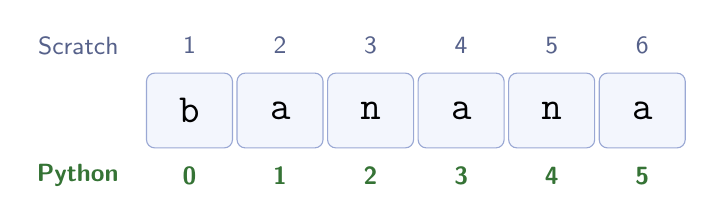
\begin{tikzpicture}[x=1.15cm]
  \foreach \l [count=\i from 0] in {b,a,n,a,n,a}{
    \draw[codeframe, fill=codebg, rounded corners=3pt] (\i,0) rectangle ++(0.95,0.95);
    \node[font=\ttfamily\Large] at (\i+0.475,0.475) {\l};
    \node[font=\small\bfseries, text=operators!60!black] at (\i+0.475,-0.35) {\i};
    \pgfmathtruncatemacro{\s}{\i+1}
    \node[font=\small, text=muted] at (\i+0.475,1.3) {\s};
  }
  \node[anchor=east, font=\small, text=muted] at (-0.2,1.3) {Scratch};
  \node[anchor=east, font=\small\bfseries, text=operators!60!black] at (-0.2,-0.35) {Python};
\end{tikzpicture}
\end{center}

\begin{watchout}[Watch out: off the end]
\texttt{"banana"} has 6 letters, so the last one is \py|word[5]|. Asking for \py|word[6]| stops with \texttt{IndexError: string index out of range}. (Scratch just gives an empty answer.) \textbf{Bonus:} \py|word[-1]| is a shortcut for the last letter.
\end{watchout}

% ---------------------------------------------------------------------
\needspace{15\baselineskip}
\subsection*{Contains}

\begin{tcbraster}[raster columns=2, raster equal height=rows, raster column skip=12pt, raster valign=center, raster force size=false, raster odd column/.style={add to width=-1.2cm}, raster even column/.style={add to width=1.2cm}]
\begin{tcolorbox}[colback=white, colframe=white, boxrule=0pt, valign=center]
\begin{scratch}
\blockinit{when \greenflag clicked}
\blocklook{say \booloperator{\ovalnum{banana} contains \ovalnum{nan} ?}}
\end{scratch}
\end{tcolorbox}
\begin{code}
print("nan" in "banana")
\end{code}
\end{tcbraster}

\textbf{How it works.} It shows \texttt{True}. Read it out loud: ``is \texttt{nan} \textbf{in} \texttt{banana}?'' The order is flipped from Scratch: the small piece comes first, then \py|in|, then the big word. Like \texttt{==}, \py|in| cares about capitals: \py|"A" in "banana"| is \py|False|. Use \py|.lower()| again if you need it.

% ---------------------------------------------------------------------
\needspace{15\baselineskip}
\subsection*{Mod: the leftover}

\begin{tcbraster}[raster columns=2, raster equal height=rows, raster column skip=12pt, raster valign=center, raster force size=false, raster odd column/.style={add to width=-1.2cm}, raster even column/.style={add to width=1.2cm}]
\begin{tcolorbox}[colback=white, colframe=white, boxrule=0pt, valign=center]
\begin{scratch}
\blockinit{when \greenflag clicked}
\blocklook{say \ovaloperator{\ovalnum{7} mod \ovalnum{3}} for \ovalnum{1} seconds}
\blocklook{say \booloperator{\ovaloperator{\ovalnum{10} mod \ovalnum{2}} = \ovalnum{0}}}
\end{scratch}
\end{tcolorbox}
\begin{tcolorbox}[colback=white, colframe=white, boxrule=0pt, left=0pt, right=0pt, top=0pt, bottom=0pt, valign=center]
\begin{code}
print(7 % 3)
print(10 % 2 == 0)
\end{code}
\begin{outputbox}
1\\
True
\end{outputbox}
\end{tcolorbox}
\end{tcbraster}

\textbf{How it works.} In Python, \texttt{mod} is the percent sign, \texttt{\%}. It gives the \textbf{leftover} after dividing. Share 7 sweets between 3 friends: everyone gets 2, and 1 is left over. So \py|7 % 3| is 1.

\begin{think}[Even or odd?]
An even number divided by 2 has nothing left over. So \py|n % 2 == 0| is \py|True| for even numbers and \py|False| for odd ones. Programmers use this trick all the time.
\end{think}

% ---------------------------------------------------------------------
\needspace{15\baselineskip}
\subsection*{abs, square root and friends}

\begin{tcbraster}[raster columns=2, raster equal height=rows, raster column skip=12pt, raster valign=center, raster force size=false, raster odd column/.style={add to width=-1.2cm}, raster even column/.style={add to width=1.2cm}]
\begin{tcolorbox}[colback=white, colframe=white, boxrule=0pt, valign=center]
\begin{scratch}
\blockinit{when \greenflag clicked}
\blocklook{say \ovaloperator{\selectmenu{abs} of \ovalnum{-5}} for \ovalnum{1} seconds}
\blocklook{say \ovaloperator{\selectmenu{sqrt} of \ovalnum{16}}}
\end{scratch}
\end{tcolorbox}
\begin{tcolorbox}[colback=white, colframe=white, boxrule=0pt, left=0pt, right=0pt, top=0pt, bottom=0pt, valign=center]
\begin{code}
import math
print(abs(-5))
print(math.sqrt(16))
\end{code}
\begin{outputbox}
5\\
4.0
\end{outputbox}
\end{tcolorbox}
\end{tcbraster}

\textbf{How it works.} \py|abs( )| takes away the minus sign. It is built into Python, so you can use it straight away. The square root lives in Python's maths tools, so first \py|import math|, then use \py|math.sqrt( )|. The square root of 16 is 4, because $4 \times 4 = 16$. Like divide, it gives a decimal: \texttt{4.0}.

The other choices in that Scratch drop-down are in \texttt{math} too: \chip[operators]{floor of} is \py|math.floor( )| (round down) and \chip[operators]{ceiling of} is \py|math.ceil( )| (round up). The angle ones, like \texttt{sin}, work a bit differently in Python, so leave them for later.

% ---------------------------------------------------------------------
\needspace{15\baselineskip}
\subsection*{Round}

\begin{tcbraster}[raster columns=2, raster equal height=rows, raster column skip=12pt, raster valign=center, raster force size=false, raster odd column/.style={add to width=-1.2cm}, raster even column/.style={add to width=1.2cm}]
\begin{tcolorbox}[colback=white, colframe=white, boxrule=0pt, valign=center]
\begin{scratch}
\blockinit{when \greenflag clicked}
\blocklook{say \ovaloperator{round \ovalnum{2.7}} for \ovalnum{1} seconds}
\blocklook{say \ovaloperator{round \ovalnum{2.5}}}
\end{scratch}
\end{tcolorbox}
\begin{tcolorbox}[colback=white, colframe=white, boxrule=0pt, left=0pt, right=0pt, top=0pt, bottom=0pt, valign=center]
\begin{code}
print(round(2.7))
print(round(2.5))
\end{code}
\begin{outputbox}
3\\
2
\end{outputbox}
\end{tcolorbox}
\end{tcbraster}

\textbf{How it works.} \py|round( )| goes to the nearest whole number, so 2.7 becomes 3. But look at the second answer!

\begin{watchout}[Watch out: Python rounds 2.5 to 2]
Scratch rounds 2.5 \textbf{up} to 3. Python rounds a number that ends in .5 to the nearest \textbf{even} number. So \py|round(2.5)| is 2, but \py|round(3.5)| is 4. Grown-up programmers do this so that, over lots of numbers, rounding doesn't push the total up.

Want Scratch's way? Use \py|math.floor(2.5 + 0.5)|, which gives \texttt{3}.

\textbf{Bonus:} \py|round(3.14159, 2)| keeps 2 decimal places and gives \texttt{3.14}.
\end{watchout}

% ---------------------------------------------------------------------
\needspace{15\baselineskip}
\subsection*{Python is fussier than Scratch}

Here are all the robot-chef moments from this part in one table. Come back to it when Python shows you a red error.

\begin{center}\small
\renewcommand{\arraystretch}{1.35}
\begin{tabular}{P{3.6cm} P{2.3cm} P{3.7cm} P{5.2cm}}
\toprule
\textbf{You write} & \textbf{Scratch says} & \textbf{Python says} & \textbf{Do this instead} \\
\midrule
\texttt{"Score: " + 10} & Score: 10 & \texttt{TypeError} & \py|"Score: " + str(10)| \\
\texttt{"Cat" == "cat"} & true & \texttt{False} & \py|.lower()| on both \\
letter 1 of \texttt{"cat"} & c & \py|"cat"[1]| is \texttt{a} & \py|"cat"[0]| \\
round 2.5 & 3 & \texttt{2} & \py|math.floor(2.5 + 0.5)| \\
\texttt{10 / 0} & Infinity & \texttt{ZeroDivisionError} & Never divide by 0 \\
pick random 6 to 1 & a number & \texttt{ValueError} & Smaller number first \\
\bottomrule
\end{tabular}
\end{center}

\needspace{16\baselineskip}
\subsection*{Predict it!}
Before you run each line, write down what you think Python will show. Then type all six lines into one cell and run it. How many did you get right? (Answers at the back.)

\begin{center}
\renewcommand{\arraystretch}{1.6}
\begin{tabular}{l P{5cm}}
\toprule
\textbf{Code} & \textbf{I think it shows} \\
\midrule
\py|print(9 / 3)| & \rule{4cm}{0.4pt} \\
\py|print("4" + "4")| & \rule{4cm}{0.4pt} \\
\py|print("Dog" == "dog")| & \rule{4cm}{0.4pt} \\
\py|print("pizza"[1])| & \rule{4cm}{0.4pt} \\
\py|print(round(4.5))| & \rule{4cm}{0.4pt} \\
\py|print(17 % 5)| & \rule{4cm}{0.4pt} \\
\bottomrule
\end{tabular}
\end{center}

% =====================================================================
\setscratch{scale=0.7}
\mission{Dice roller}{\texttt{random.randint}, adding up in a loop, and joining numbers with \texttt{str( )}}

Roll a dice 10 times, add up all the rolls, and work out the average. Is the average close to what you expected?

\step{Step 1: Build it in Scratch}
Make two variables, \textbf{roll} and \textbf{total}, then build:

\begin{center}
\begin{scratch}
\blockinit{when \greenflag clicked}
\blockvariable{set \selectmenu{total} to \ovalnum{0}}
\blockrepeat{repeat \ovalnum{10}}{
  \blockvariable{set \selectmenu{roll} to \ovaloperator{pick random \ovalnum{1} to \ovalnum{6}}}
  \blockvariable{change \selectmenu{total} by \ovalvariable{roll}}
  \blocklook{say \ovaloperator{join \ovalnum{You rolled } \ovalvariable{roll}} for \ovalnum{1} seconds}
}
\blocklook{say \ovaloperator{join \ovalnum{Total: } \ovalvariable{total}} for \ovalnum{2} seconds}
\blocklook{say \ovaloperator{join \ovalnum{Average: } \ovaloperator{\ovalvariable{total} / \ovalnum{10}}}}
\end{scratch}
\end{center}

\step{Step 2: Type it in Colab}

\begin{typethis}
import random
total = 0
for i in range(10):
    roll = random.randint(1, 6)
    total = total + roll
    print("You rolled " + str(roll))
print("Total: " + str(total))
print("Average: " + str(total / 10))
\end{typethis}

\step{Step 3: Read it line by line}

\begin{longtable}{>{\centering\arraybackslash}p{1.1cm} P{5.3cm} P{9.1cm}}
\toprule
\textbf{Line} & \textbf{Scratch block} & \textbf{What it means} \\
\midrule
--- & \chip[events]{when green flag clicked} & No code needed: the play button \playbtn{} starts it. \\
1 & (Extensions) & Brings in the random tools. \\
2 & \chip[variables]{set total to 0} & Make a box called \py|total| with 0 in it. \\
3 & \chip[control]{repeat 10} & Do the indented lines 10 times. \\
4 & \chip[variables]{set roll to pick random} & Roll the dice: a whole number from 1 to 6, both ends included. \\
5 & \chip[variables]{change total by roll} & Take what is in \py|total|, add the roll, and put the answer back in \py|total|. \\
6 & \chip[looks]{say join You rolled roll} & \py|roll| is a number, so \py|str(roll)| turns it into a string before joining. \\
7 & \chip[looks]{say join Total: total} & No spaces in front, so this runs once, after the loop. \\
8 & \chip[looks]{say join Average: \ldots} & \py|total / 10| is worked out first, then turned into a string. \\
\bottomrule
\end{longtable}

\step{Step 4: Run it}
Press \playbtn. Your rolls will be different, because they are random! Here is one real run:

\begin{outputbox}[You might see]
You rolled 6\\
You rolled 2\\
{\sffamily\itshape\color{muted} \ldots\ 8 more rolls: 6, 2, 1, 3, 3, 1, 4, 6 \ldots}\\
Total: 34\\
Average: 3.4
\end{outputbox}

The average is a decimal because \texttt{/} always gives a decimal. If you roll a fair dice lots and lots of times, the average gets close to 3.5, exactly half-way between 1 and 6.

\begin{challenge}
\tick Roll 100 times instead of 10. Change line 3 \textbf{and} line 8. Is the average closer to 3.5 now? (Tip: take out line 6 first, or you will get 100 lines!)\par
\tick Make a 20-sided dice for a board game.\par
\tick Roll \textbf{two} dice each time: \py|roll = random.randint(1, 6) + random.randint(1, 6)|. What is the biggest total you could get?\par
\tick Add \py|print(roll == 6)| inside the loop. It shows \texttt{True} every time you roll a six.
\end{challenge}

% =====================================================================
\mission{Times-table printer}{multiplying in a loop, and f-strings}

Let Python print a whole times table in a flash. Then change one number to get any table you like.

\step{Step 1: Build it in Scratch}
Make two variables, \textbf{table} and \textbf{n}, then build:

\begin{center}
\begin{scratch}
\blockinit{when \greenflag clicked}
\blockvariable{set \selectmenu{table} to \ovalnum{7}}
\blockvariable{set \selectmenu{n} to \ovalnum{1}}
\blockrepeat{repeat \ovalnum{12}}{
  \blocklook{say \ovaloperator{join \ovalvariable{n} \ovaloperator{join \ovalnum{ x 7 = } \ovaloperator{\ovalvariable{n} * \ovalvariable{table}}}} for \ovalnum{1} seconds}
  \blockvariable{change \selectmenu{n} by \ovalnum{1}}
}
\end{scratch}
\end{center}

That's a lot of joins! Python makes this much easier.

\step{Step 2: Type it in Colab}

\begin{typethis}
table = 7
n = 1
for i in range(12):
    print(f"{n} x {table} = {n * table}")
    n = n + 1
\end{typethis}

\step{Step 3: Read it line by line}

\begin{longtable}{>{\centering\arraybackslash}p{1.1cm} P{5.3cm} P{9.1cm}}
\toprule
\textbf{Line} & \textbf{Scratch block} & \textbf{What it means} \\
\midrule
1 & \chip[variables]{set table to 7} & Which times table to print. \\
2 & \chip[variables]{set n to 1} & \py|n| counts 1, 2, 3 \ldots\ up to 12. \\
3 & \chip[control]{repeat 12} & Do the indented lines 12 times. \\
4 & \chip[looks]{say join \ldots} & An \textbf{f-string}. Each pair of curly brackets is a gap that Python fills in. \texttt{\{n * table\}} even does the sum first! The \texttt{x} is just a letter x in the writing. \\
5 & \chip[variables]{change n by 1} & Add 1 to \py|n|, ready for the next line. \\
\bottomrule
\end{longtable}

\step{Step 4: Run it}

\begin{outputbox}
1 x 7 = 7\\
2 x 7 = 14\\
3 x 7 = 21\\
4 x 7 = 28\\
{\sffamily\itshape\color{muted} \ldots\ and so on, down to \ldots}\\
12 x 7 = 84
\end{outputbox}

\begin{think}[The same line without an f-string]
You could also join with \texttt{+} and \py|str( )|, like Mission 1. It works, but it is long, so it is easier in three lines:
\begin{codenonum}
a = str(n) + " x "
b = str(table) + " = "
print(a + b + str(n * table))
\end{codenonum}
Both ways are right. Most Python coders choose the f-string.
\end{think}

\begin{challenge}
\tick Print the 9 times table. Which line do you change?\par
\tick Go all the way up to 20 x 7.\par
\tick Print square numbers: change line 4 so it shows \texttt{5 x 5 = 25} and so on. (Hint: you only need \py|n|.)\par
\tick Add \texttt{\{n * table \% 2 == 0\}} at the end of the f-string. What does the \texttt{True} or \texttt{False} tell you?
\end{challenge}

% =====================================================================
\mission{Random dot art}{random positions with \texttt{goto}, \texttt{dot( )}, and picking a random colour from a list}

The turtle jumps to 50 random places on the stage and leaves a coloured dot at each one. Every time you run it, you get a new picture!

\step{Step 1: Build it in Scratch}
Add the \textbf{Pen} extension, then build:

\begin{center}
\begin{scratch}
\blockinit{when \greenflag clicked}
\blockpen{erase all}
\blockpen{pen up}
\blocklook{hide}
\blockrepeat{repeat \ovalnum{50}}{
  \blockmove{go to x: \ovaloperator{pick random \ovalnum{-240} to \ovalnum{240}} y: \ovaloperator{pick random \ovalnum{-180} to \ovalnum{180}}}
  \blockpen{set pen size to \ovaloperator{pick random \ovalnum{10} to \ovalnum{40}}}
  \blockpen{set pen \selectmenu{color} to \ovaloperator{pick random \ovalnum{0} to \ovalnum{100}}}
  \blockpen{pen down}
  \blockpen{pen up}
}
\end{scratch}
\end{center}

\step{Step 2: Type it in Colab}

\begin{typethis}
from ColabTurtlePlus.Turtle import *
clearscreen()
initializeTurtle((480, 360))
import random

colours = ["red", "gold", "skyblue", "pink", "lime"]
speed(13)
penup()
hideturtle()
for i in range(50):
    x = random.randint(-240, 240)
    y = random.randint(-180, 180)
    goto(x, y)
    size = random.randint(10, 40)
    colour = colours[random.randint(0, 4)]
    dot(size, colour)
\end{typethis}

\step{Step 3: Read it line by line}

\begin{longtable}{>{\centering\arraybackslash}p{1.1cm} P{5.3cm} P{9.1cm}}
\toprule
\textbf{Line} & \textbf{Scratch block} & \textbf{What it means} \\
\midrule
1--3 & \chip[events]{when green flag clicked}\newline\chip[pen]{erase all} & The three starting lines. They also wipe the stage clean. \\
4 & (Extensions) & Bring in the random tools. \\
6 & (a list) & A list of 5 colour names. Scratch pen colours are numbers from 0 to 100, but Python likes colour \textbf{names}, so we keep our favourites in a list. \\
7 & & Draw as fast as the turtle can go. \\
8--9 & \chip[pen]{pen up}\newline\chip[looks]{hide} & Don't draw lines between the dots, and hide the turtle. \\
10 & \chip[control]{repeat 50} & Make 50 dots. \\
11--13 & \chip[motion]{go to x: \ldots{} y: \ldots} & Pick a random \py|x| from one side of the stage to the other, and a random \py|y| from bottom to top. Then go there. \\
14 & \chip[pen]{set pen size to pick random} & A random dot size from 10 to 40. \\
15 & \chip[pen]{set pen color to pick random} & Pick a random place in the list. The list has 5 colours, but Python counts from 0, so the places are 0, 1, 2, 3 and 4. That's why it is \py|randint(0, 4)| and not \py|randint(1, 5)|. \\
16 & \chip[pen]{pen down}\newline\chip[pen]{pen up} & In Scratch, pen down then pen up makes a dot. \py|dot(size, colour)| draws a round dot right where the turtle is. \\
\bottomrule
\end{longtable}

\step{Step 4: Run it}
You should see 50 dots of different sizes in red, gold, sky blue, pink and lime, scattered all over the stage. Run it again: the picture is different every time.

\begin{challenge}
\tick Add \py|bgcolor("black")| after line 3 for a night sky. Make 200 dots.\par
\tick Add more colours to the list, such as \py|"orange"| and \py|"purple"|. Line 15 only picks places 0 to 4, so it will never pick them until you fix it. (Clever way: \py|random.randint(0, len(colours) - 1)| always fits the list.)\par
\tick Make all the dots fall in the top half of the stage. Which numbers in line 12 do you change?\par
\tick \textbf{Bonus:} \py|random.choice(colours)| picks a random item from a list in one go. Try it in line 15.
\end{challenge}

% =====================================================================
\mission{Name machine}{taking words apart with letters and \texttt{len( )}, and building a word backwards}

Python takes a name, counts its letters, spells it out one letter per line, and then writes it backwards.

\step{Step 1: Build it in Scratch}
Make three variables, \textbf{name}, \textbf{n} and \textbf{backwards}, then build:

\begin{center}
\begin{scratch}
\blockinit{when \greenflag clicked}
\blockvariable{set \selectmenu{name} to \ovalnum{Matilda}}
\blocklook{say \ovaloperator{join \ovalnum{Your name has } \ovaloperator{join \ovaloperator{length of \ovalvariable{name}} \ovalnum{ letters}}} for \ovalnum{2} seconds}
\blockvariable{set \selectmenu{n} to \ovalnum{1}}
\blockrepeat{repeat \ovaloperator{length of \ovalvariable{name}}}{
  \blocklook{say \ovaloperator{letter \ovalvariable{n} of \ovalvariable{name}} for \ovalnum{1} seconds}
  \blockvariable{change \selectmenu{n} by \ovalnum{1}}
}
\blockvariable{set \selectmenu{backwards} to \ovalnum{}}
\blockvariable{set \selectmenu{n} to \ovalnum{1}}
\blockrepeat{repeat \ovaloperator{length of \ovalvariable{name}}}{
  \blockvariable{set \selectmenu{backwards} to \ovaloperator{join \ovaloperator{letter \ovalvariable{n} of \ovalvariable{name}} \ovalvariable{backwards}}}
  \blockvariable{change \selectmenu{n} by \ovalnum{1}}
}
\blocklook{say \ovalvariable{backwards}}
\end{scratch}
\end{center}

\step{Step 2: Type it in Colab}
Put your own name in line 1!

\begin{typethis}
name = "Matilda"
print("Your name has " + str(len(name)) + " letters")
for i in range(len(name)):
    print(name[i])

backwards = ""
for i in range(len(name)):
    backwards = name[i] + backwards
print(backwards)
\end{typethis}

\step{Step 3: Read it line by line}

\begin{longtable}{>{\centering\arraybackslash}p{1.1cm} P{5.3cm} P{9.1cm}}
\toprule
\textbf{Line} & \textbf{Scratch block} & \textbf{What it means} \\
\midrule
1 & \chip[variables]{set name to Matilda} & The name goes in quote marks, because it is a string. \\
2 & \chip[looks]{say join Your name has \ldots} & \py|len(name)| counts the letters. \py|str( )| turns that number into a string, so it can be joined. \\
3 & \chip[control]{repeat length of name} & Go round once for every letter. \\
4 & \chip[looks]{say letter n of name} & Here is the clever part. The loop's \py|i| counts 0, 1, 2, 3 \ldots\ and those are exactly the numbers Python uses for letters! So Python doesn't need \texttt{n} or \chip[variables]{change n by 1}. \\
6 & \chip[variables]{set backwards to (empty)} & Two quote marks with nothing between them make an empty string, like an empty box. \\
7 & \chip[control]{repeat length of name} & Go through the letters again. \\
8 & \chip[variables]{set backwards to join \ldots} & Stick each new letter on the \textbf{front}. M, then aM, then taM \ldots\ until the whole name is backwards. \\
9 & \chip[looks]{say backwards} & Show the backwards name, once, after the loop. \\
\bottomrule
\end{longtable}

\step{Step 4: Run it}

\begin{outputbox}
Your name has 7 letters\\
M\\
a\\
t\\
i\\
l\\
d\\
a\\
adlitaM
\end{outputbox}

\begin{think}[Spaces are letters too]
Try \py|name = "Ada Lovelace"|. Python says it has 12 letters, because it counts the space too. Scratch's \chip[operators]{length of} does the same.
\end{think}

\begin{challenge}
\tick Print the name in capitals with \py|print(name.upper())|.\par
\tick Print the first and the last letter: \py|name[0]| and \py|name[-1]|.\par
\tick Number the letters: change line 4 to \py|print(str(i + 1) + ": " + name[i])|. Why does it say \py|i + 1|?\par
\tick Does your name contain an \texttt{a}? Add \py|print("a" in name.lower())|.
\end{challenge}

% =====================================================================
\needspace{22\baselineskip}
\subsection*{Part 4: Translate it yourself}

Here is a Scratch script you haven't seen. Write it in Python on the lines, then type it into Colab and run it. Does it do the same as the Scratch script? (Answer at the back.)

\begin{tcbraster}[raster columns=2, raster equal height=rows, raster column skip=12pt, raster valign=top]
\begin{tcolorbox}[colback=white, colframe=white, boxrule=0pt]
\begin{scratch}
\blockinit{when \greenflag clicked}
\blockrepeat{repeat \ovalnum{3}}{
  \blockvariable{set \selectmenu{a} to \ovaloperator{pick random \ovalnum{1} to \ovalnum{10}}}
  \blockvariable{set \selectmenu{b} to \ovaloperator{pick random \ovalnum{1} to \ovalnum{10}}}
  \blocklook{say \ovaloperator{join \ovalnum{Total: } \ovaloperator{\ovalvariable{a} + \ovalvariable{b}}} for \ovalnum{1} seconds}
}
\end{scratch}
\end{tcolorbox}
\begin{tcolorbox}[colback=white, colframe=codeframe, arc=5pt, title=\textbf{My Python}, coltitle=ink, colbacktitle=codebg]
\vspace{4pt}
\foreach \n in {1,...,7}{\rule{\linewidth}{0.4pt}\par\vspace{9pt}}
\end{tcolorbox}
\end{tcbraster}

\textbf{Two clues:} what do you need at the very top before you can pick random numbers? And can you join \texttt{"Total: "} straight to a number?

\begin{puzzle}
The turtle's secret password is the \textbf{first letter} of \texttt{Turtle} joined to the \textbf{number of letters} in \texttt{Turtle}. Write \textbf{two lines} of Python that work out the password and print it. Don't type the answer in yourself: make Python work it out!

When it works, you should see:
\begin{outputbox}
T6
\end{outputbox}
\end{puzzle}

\setscratch{scale=1}
\needspace{8\baselineskip}
\subsection*{Part 4 checklist}
\tick I can do sums with \texttt{+ - * /}, and I know \texttt{/} always gives a decimal.\par
\tick I can pick a random number with \py|random.randint( )|, after \py|import random|.\par
\tick I can compare with \texttt{> < ==} and \py|and|, \py|or|, \py|not|, and print \py|True| or \py|False|.\par
\tick I can join strings with \texttt{+}, and use \py|str( )| or an f-string for numbers.\par
\tick I can get a letter with \py|word[0]|, count letters with \py|len( )|, and check with \py|in|.\par
\tick I know where Python is fussier than Scratch: \py|round(2.5)|, capitals and counting from 0.

% =====================================================================
% PART 5: Sensing and Decisions
% =====================================================================
\partopener{sensing}{PART 5}{Sensing and Decisions}{Your programs will listen to you, watch the clock and make choices.}

Until now your programs did the same thing every time you pressed \playbtn. In this part they start to \textbf{sense} things and \textbf{decide} what to do. Sensing blocks are the sprite's eyes, ears and watch. In Python, \py|input()| is the program's ears, \py|distance()| is its measuring tape, and \py|time| is its stopwatch.

You will meet these Scratch blocks and their Python twins:

\begin{itemize}
  \item \chip[sensing]{ask and wait} and \chip[sensing]{answer} become \py|input()|
  \item \chip[control]{if then}, \chip[control]{if then else} and \chip[control]{repeat until} become \py|if|, \py|else| and \py|while|
  \item \chip[sensing]{timer} and \chip[sensing]{current year} become \py|time| and \py|datetime|
  \item \chip[sensing]{touching?} and \chip[motion]{if on edge, bounce} become a little bit of maths with \py|distance()|, \py|xcor()| and \py|if|
\end{itemize}

None of these programs need the turtle until near the end, so most of them start straight away with no starting lines.

% ---------------------------------------------------------------------
\needspace{14\baselineskip}
\subsection*{Ask a question and wait}

\begin{tcbraster}[raster columns=2, raster equal height=rows, raster column skip=12pt, raster valign=center, raster force size=false, raster column 1/.style={width=0.36\linewidth}, raster column 2/.style={width=0.64\linewidth-12pt}]
\begin{tcolorbox}[colback=white, colframe=white, boxrule=0pt, valign=center, left=0pt, right=0pt]
\setscratch{scale=0.8}
\begin{scratch}
\blockinit{when \greenflag clicked}
\blocksensing{ask \ovalnum{What's your name?} and wait}
\blocklook{say \ovaloperator{join \ovalnum{Hello } \ovalsensing{answer}}}
\end{scratch}
\end{tcolorbox}
\begin{code}
name = input("What's your name? ")
print("Hello " + name)
\end{code}
\end{tcbraster}

\textbf{How it works.} \py|input("...")| does the job of \chip[sensing]{ask and wait}. It shows the question, then a little box appears \textbf{under the cell}. Click in the box, type, and press \textbf{Enter}. Whatever you typed comes out of \py|input()| and is put into the variable on the left of the \texttt{=}. Scratch keeps the reply in a block called \chip[sensing]{answer}; in Python \textbf{you} choose the name of the box, so here it is called \py|name|.

\begin{outputbox}
What's your name? Ada\\
Hello Ada
\end{outputbox}

\begin{think}[Leave a space at the end]
Look at the space after the question mark in \py|"What's your name? "|. It stops your typing from sticking to the question, like \texttt{What's your name?Ada}.
\end{think}

% ---------------------------------------------------------------------
\needspace{14\baselineskip}
\subsection*{Input always gives you writing}

\begin{center}
\begin{scratch}
\blockinit{when \greenflag clicked}
\blocksensing{ask \ovalnum{How old are you?} and wait}
\blocklook{say \ovaloperator{join \ovalnum{Next year you will be } \ovaloperator{\ovalsensing{answer} + \ovalnum{1}}}}
\end{scratch}
\end{center}
\vspace{-4pt}
\begin{code}
age = input("How old are you? ")
age = int(age)
print("Next year you will be " + str(age + 1))
\end{code}

\textbf{How it works.} Whatever you type into \py|input()| is \textbf{writing} to Python, even if it looks like a number. \texttt{"9"} is writing; \texttt{9} is a number. Scratch quietly turns the writing into a number for you. Python wants you to say so: \py|int(age)| turns the writing \texttt{"9"} into the number \texttt{9}. (\texttt{int} is short for \emph{integer}, which means a whole number.) Then \py|str( )| turns the answer back into writing so it can be joined with \texttt{+}, just as you did in Part 4.

You can do both jobs in one line, and you will see this a lot:
\begin{codenonum}
age = int(input("How old are you? "))
\end{codenonum}

\needspace{12\baselineskip}
\begin{watchout}[What if you type a word?]
Run the program and type \texttt{nine} instead of \texttt{9}. Python can't turn \texttt{nine} into a number, so it stops with a clue note. Read the \textbf{last line} first:
\begin{errorbox}
ValueError: invalid literal for int() with base 10: 'nine'
\end{errorbox}
It means: ``\texttt{int()} was given \texttt{'nine'}, and that isn't a number I can read.'' Nothing is broken. Press \playbtn{} again and type digits.
\end{watchout}

% ---------------------------------------------------------------------
\needspace{14\baselineskip}
\subsection*{If this, then that}

\begin{tcbraster}[raster columns=2, raster equal height=rows, raster column skip=12pt, raster valign=center, raster force size=false, raster column 1/.style={width=0.36\linewidth}, raster column 2/.style={width=0.64\linewidth-12pt}]
\begin{tcolorbox}[colback=white, colframe=white, boxrule=0pt, valign=center, left=0pt, right=0pt]
\setscratch{scale=0.8}
\begin{scratch}
\blockinit{when \greenflag clicked}
\blocksensing{ask \ovalnum{Do you like cats?} and wait}
\blockif{if \booloperator{\ovalsensing{answer} = \ovalnum{yes}} then}{
  \blocklook{say \ovalnum{Me too!} for \ovalnum{2} seconds}
}
\blocklook{say \ovalnum{Bye!}}
\end{scratch}
\end{tcolorbox}
\begin{code}
answer = input("Do you like cats? ")
if answer == "yes":
    print("Me too!")
print("Bye!")
\end{code}
\end{tcbraster}

\textbf{How it works.} \py|if| works just like the C-shaped \chip[control]{if then} block. The \textbf{colon} at the end opens the mouth of the C, and the lines with \textbf{four spaces} in front go inside it, exactly like a \py|for| loop. Python checks the question once. If it is true, it runs the inside lines; if not, it skips them. \py|print("Bye!")| is back at the left edge, so it is \textbf{under} the C and always runs. Remember: \textbf{two} equals signs \texttt{==} \textbf{check}; one \texttt{=} \textbf{sets}.

\begin{watchout}[Capitals count]
Type \texttt{Yes} with a capital Y. Python says only \texttt{Bye!}, because \texttt{"Yes"} and \texttt{"yes"} are different to Python. Scratch thinks they are the same! You will learn the fix, \py|.lower()|, in Mission 3.
\end{watchout}

% ---------------------------------------------------------------------
\needspace{14\baselineskip}
\subsection*{If this, else that}

\begin{tcbraster}[raster columns=2, raster equal height=rows, raster column skip=12pt, raster valign=center, raster force size=false, raster column 1/.style={width=0.36\linewidth}, raster column 2/.style={width=0.64\linewidth-12pt}]
\begin{tcolorbox}[colback=white, colframe=white, boxrule=0pt, valign=center, left=0pt, right=0pt]
\setscratch{scale=0.8}
\begin{scratch}
\blockinit{when \greenflag clicked}
\blocksensing{ask \ovalnum{How old are you?} and wait}
\blockifelse{if \booloperator{\ovalsensing{answer} > \ovalnum{9}} then}{
  \blocklook{say \ovalnum{Double figures!}}
}{
  \blocklook{say \ovalnum{Not double figures yet}}
}
\end{scratch}
\end{tcolorbox}
\begin{code}
age = int(input("How old are you? "))
if age >= 10:
    print("Double figures!")
else:
    print("Not double figures yet")
\end{code}
\end{tcbraster}

\textbf{How it works.} \py|else:| is the second mouth of the \chip[control]{if then else} block. It means ``otherwise''. \py|else| lines up with \py|if| (no spaces in front) and needs its own colon. Exactly \textbf{one} of the two mouths runs, never both. Scratch has no ``bigger or equal'' block, so Scratch uses \texttt{> 9}; Python can say \py|>= 10| (``10 or more''). Both mean the same thing for whole numbers.

% ---------------------------------------------------------------------
\needspace{14\baselineskip}
\subsection*{A Python shortcut: elif}

\begin{center}
\setscratch{scale=0.8}
\begin{scratch}
\blocksensing{ask \ovalnum{Your score out of 10?} and wait}
\blockifelse{if \booloperator{\ovalsensing{answer} = \ovalnum{10}} then}{
  \blocklook{say \ovalnum{Perfect!}}
}{
  \blockifelse{if \booloperator{\ovalsensing{answer} > \ovalnum{6}} then}{
    \blocklook{say \ovalnum{Great job!}}
  }{
    \blockifelse{if \booloperator{\ovalsensing{answer} > \ovalnum{3}} then}{
      \blocklook{say \ovalnum{Good try!}}
    }{
      \blocklook{say \ovalnum{Keep practising!}}
    }
  }
}
\end{scratch}
\end{center}
\vspace{-4pt}
\begin{code}
score = int(input("Your score out of 10? "))
if score == 10:
    print("Perfect!")
elif score >= 7:
    print("Great job!")
elif score >= 4:
    print("Good try!")
else:
    print("Keep practising!")
\end{code}

\textbf{How it works.} In Scratch, to choose between more than two things you put an \chip[control]{if then else} inside the \textbf{else} mouth of another one, and the script gets wider and wider. Python has a shortcut that Scratch doesn't: \py|elif|, short for ``else if''. Python checks the questions \textbf{from the top} and runs only the \textbf{first} one that is true, then jumps past all the rest. If none is true, the \py|else| part runs. All the \py|if|, \py|elif| and \py|else| lines line up, so the code stays neat and narrow.

\begin{think}[Why does 8 not say ``Good try!'' too?]
8 is bigger than 4, so \py|score >= 4| is true. But Python already found \py|score >= 7| was true, ran \texttt{Great job!}, and skipped everything below it. Only one part ever runs.
\end{think}

% ---------------------------------------------------------------------
\needspace{14\baselineskip}
\subsection*{Repeat until: Python flips the question}

\begin{tcbraster}[raster columns=1, raster row skip=6pt]
\begin{tcolorbox}[colback=white, colframe=white, boxrule=0pt, valign=center, left=0pt, right=0pt]
\setscratch{scale=0.8}
\begin{scratch}
\blockinit{when \greenflag clicked}
\blockrepeat{repeat until \booloperator{\ovalsensing{answer} = \ovalnum{Genesis}}}{
  \blocksensing{ask \ovalnum{First book of the Bible?} and wait}
}
\blocklook{say \ovalnum{Well done!}}
\end{scratch}
\end{tcolorbox}
\begin{code}
answer = ""
while answer != "Genesis":
    answer = input("First book of the Bible? ")
print("Well done!")
\end{code}
\end{tcbraster}

\textbf{How it works.} Python has no ``repeat until''. It has \py|while|, which means ``keep going \textbf{as long as} this is true''. So you flip the question. Scratch says repeat \textbf{until} the answer \textbf{is} ``Genesis''. Python says keep going \textbf{while} the answer is \textbf{not} ``Genesis''. \texttt{!=} means ``is not equal to''. It is like ``stay outside until it rains'' and ``stay outside while it isn't raining'': the same plan, said the other way round.

You can also flip it with the word \py|not|, which matches the green \chip[operators]{not} block:
\begin{codenonum}
while not answer == "Genesis":
\end{codenonum}
Both lines do the same thing. Most Python coders use \texttt{!=} because it is shorter.

\begin{think}[Why \texttt{answer = ""} on line 1?]
\py|while| checks its question \textbf{before} the first go, just like \chip[control]{repeat until}. Python needs a box called \py|answer| to look in. \py|""| is empty writing: a box with nothing in it yet. It is not ``Genesis'', so the loop starts.
\end{think}

% ---------------------------------------------------------------------
\needspace{14\baselineskip}
\subsection*{Your own stopwatch: the timer}

\begin{center}
\begin{scratch}
\blockinit{when \greenflag clicked}
\blocksensing{reset timer}
\blocksensing{ask \ovalnum{Count to 10, then press Enter} and wait}
\blocklook{say \ovaloperator{join \ovalnum{That took } \ovalsensing{timer}}}
\end{scratch}
\end{center}
\vspace{-4pt}
\begin{code}
import time
start = time.time()
input("Count to 10 in your head, then press Enter ")
taken = time.time() - start
print("That took " + str(round(taken, 1)) + " seconds")
\end{code}

\textbf{How it works.} Python has no timer that starts by itself. Instead, \py|time.time()| tells you what time it is right now, as a huge number of seconds. (It counts from 1 January 1970!) So you make your own stopwatch: write down the time at the start (\py|start = time.time()|, that is \chip[sensing]{reset timer}), and later take it away from the new time. \py|time.time() - start| is the \chip[sensing]{timer} block: the seconds since you started. \py|round(taken, 1)| keeps one number after the dot.

\begin{think}[Reset the timer]
To reset your stopwatch, just do \py|start = time.time()| again. You can have lots of stopwatches at once, too: \py|start1|, \py|start2|\ldots{} Scratch has only one timer.
\end{think}

% ---------------------------------------------------------------------
\needspace{14\baselineskip}
\subsection*{Wait until}

\begin{tcbraster}[raster columns=2, raster equal height=rows, raster column skip=12pt, raster valign=center, raster force size=false, raster column 1/.style={width=0.36\linewidth}, raster column 2/.style={width=0.64\linewidth-12pt}]
\begin{tcolorbox}[colback=white, colframe=white, boxrule=0pt, valign=center, left=0pt, right=0pt]
\setscratch{scale=0.8}
\begin{scratch}
\blockinit{when \greenflag clicked}
\blocksensing{reset timer}
\blocklook{say \ovalnum{Wait for it...}}
\blockcontrol{wait until \booloperator{\ovalsensing{timer} > \ovalnum{3}}}
\blocklook{say \ovalnum{3 seconds are up!}}
\end{scratch}
\end{tcolorbox}
\begin{code}
import time
start = time.time()
print("Wait for it...")
while not time.time() - start > 3:
    time.sleep(0.1)
print("3 seconds are up!")
\end{code}
\end{tcbraster}

\textbf{How it works.} \chip[control]{wait until} is a \py|while not| loop that does nothing but wait. Each time round, \py|time.sleep(0.1)| has a tiny nap of a tenth of a second, then Python checks the question again. When the timer passes 3, the question \py|not ... > 3| is false, the loop ends, and line 6 runs. The nap stops the computer from asking ``are we there yet?'' millions of times a second.

\begin{watchout}[Something must change]
In Scratch, another sprite might make the question true. In Python only one script runs, so a \py|while| loop waits for ever if nothing inside it can change the answer. Waiting for the clock, or for an \py|input()|, is safe. If a cell runs for ever, press \stopbtn.
\end{watchout}

% ---------------------------------------------------------------------
\needspace{14\baselineskip}
\subsection*{What year is it? What time is it?}

\begin{center}
\setscratch{scale=0.85}
\begin{scratch}
\blockinit{when \greenflag clicked}
\blocklook{say \ovaloperator{join \ovalnum{The year is } \ovalsensing{current \selectmenu{year}}} for \ovalnum{2} seconds}
\blockifelse{if \booloperator{\ovalsensing{current \selectmenu{hour}} < \ovalnum{12}} then}{
  \blocklook{say \ovalnum{Good morning!}}
}{
  \blocklook{say \ovalnum{Good afternoon!}}
}
\end{scratch}
\end{center}
\vspace{-4pt}
\begin{code}
import datetime
now = datetime.datetime.now()
print("The year is " + str(now.year))
if now.hour < 12:
    print("Good morning!")
else:
    print("Good afternoon!")
\end{code}

\textbf{How it works.} \py|import datetime| brings in Python's calendar tools. \py|datetime.datetime.now()| reads the clock once and keeps the answer in \py|now|. Then \py|now.year|, \py|now.month|, \py|now.day|, \py|now.hour|, \py|now.minute| and \py|now.second| work like the menu in the \chip[sensing]{current year} block. (Yes, \texttt{datetime} is written twice: the first is the toolbox, the second is the tool inside it.)

\begin{watchout}[Colab's clock may be in another country]
Your code runs on a Google computer, which is often set to \textbf{UTC} (London's winter time), not your home time. If Colab says \texttt{Good afternoon!} at breakfast, your code is fine: the computer is just somewhere else in the world. The year and the date are almost always right.
\end{watchout}

% ---------------------------------------------------------------------
\needspace{14\baselineskip}
\subsection*{Touching? Use a measuring tape}

Now the turtle comes back. Scratch checks whether two pictures overlap. The turtle can't see pictures, but it can \textbf{measure}: \py|distance(x, y)| tells you how many steps away a spot is. If it is very close, say less than 20 steps, we say it is touching.

\begin{tcbraster}[raster columns=2, raster equal height=rows, raster column skip=12pt, raster valign=center, raster force size=false, raster column 1/.style={width=0.36\linewidth}, raster column 2/.style={width=0.64\linewidth-12pt}]
\begin{tcolorbox}[colback=white, colframe=white, boxrule=0pt, valign=center, left=0pt, right=0pt]
\setscratch{scale=0.8}
\begin{scratch}
\blockinit{when \greenflag clicked}
\blockmove{go to x: \ovalnum{-200} y: \ovalnum{0}}
\blockrepeat{repeat until \boolsensing{touching \selectmenu{Spot}?}}{
  \blockmove{move \ovalnum{10} steps}
}
\blocklook{say \ovalnum{Touched it!}}
\end{scratch}
\end{tcolorbox}
\begin{code}
from ColabTurtlePlus.Turtle import *
clearscreen()
initializeTurtle((480, 360))
dot(20, "red")
penup()
goto(-200, 0)
pendown()
while distance(0, 0) >= 20:
    forward(10)
print("Touched it!")
\end{code}
\end{tcbraster}

\textbf{How it works.} Line 4 draws a red spot in the middle, at $(0, 0)$. \py|distance(0, 0)| measures from the turtle to that spot. ``Repeat \textbf{until} touching'' flips into ``keep going \textbf{while} the distance is 20 or more''. It's like pretending each sprite has an invisible bubble around it.

\needspace{20\baselineskip}
To check whether two \textbf{sprites} touch, make a second turtle with \py|Turtle()| and measure to where it is. \py|dog.pos()| gives the dog's position, its $x$ and $y$ together.

\begin{tcbraster}[raster columns=2, raster equal height=rows, raster column skip=12pt, raster valign=center, raster force size=false, raster column 1/.style={width=0.36\linewidth}, raster column 2/.style={width=0.64\linewidth-12pt}]
\begin{tcolorbox}[colback=white, colframe=white, boxrule=0pt, valign=center, left=0pt, right=0pt]
\setscratch{scale=0.8}
\begin{scratch}
\blockinit{when \greenflag clicked}
\blockrepeat{repeat until \boolsensing{touching \selectmenu{Dog}?}}{
  \blockmove{move \ovalnum{10} steps}
}
\blocklook{say \ovalnum{Got you, dog!}}
\end{scratch}
\end{tcolorbox}
\begin{code}
from ColabTurtlePlus.Turtle import *
clearscreen()
initializeTurtle((480, 360))
shape("turtle")
dog = Turtle()
dog.shape("circle")
dog.penup()
dog.goto(150, 0)
while distance(dog.pos()) >= 20:
    forward(10)
print("Got you, dog!")
\end{code}
\end{tcbraster}

\textbf{How it works.} \py|dog = Turtle()| makes a new sprite and gives it the name \py|dog|. Commands with \py|dog.| in front move only the dog; plain commands move the first turtle, as always. Line 9 measures from the turtle to the dog's position. If you make two named sprites, the check looks like \py|cat.distance(dog.pos()) < 20|.

\begin{watchout}[Don't forget \texttt{.pos()}]
In ColabTurtlePlus you must measure to the dog's \textbf{position}, \py|dog.pos()|. Writing \py|distance(dog)| gives a \texttt{ValueError}, because the measuring tape wants numbers, not a whole sprite.
\end{watchout}

% ---------------------------------------------------------------------
\needspace{14\baselineskip}
\subsection*{Key pressed? Mouse down? Take turns instead}

\begin{tcbraster}[raster columns=2, raster equal height=rows, raster column skip=12pt, raster valign=center, raster force size=false, raster column 1/.style={width=0.36\linewidth}, raster column 2/.style={width=0.64\linewidth-12pt}]
\begin{tcolorbox}[colback=white, colframe=white, boxrule=0pt, valign=center, left=0pt, right=0pt]
\setscratch{scale=0.7}
\begin{scratch}
\blockinit{when \greenflag clicked}
\blockrepeat{repeat \ovalnum{5}}{
  \blockif{if \boolsensing{key \selectmenu{left arrow} pressed?} then}{
    \blockmove{turn \turnleft{} \ovalnum{90} degrees}
  }
  \blockif{if \boolsensing{key \selectmenu{right arrow} pressed?} then}{
    \blockmove{turn \turnright{} \ovalnum{90} degrees}
  }
  \blockmove{move \ovalnum{50} steps}
}
\end{scratch}
\end{tcolorbox}
\begin{code}
from ColabTurtlePlus.Turtle import *
clearscreen()
initializeTurtle((480, 360))
shape("turtle")
for i in range(5):
    key = input("f, l or r? ")
    if key == "l":
        left(90)
    elif key == "r":
        right(90)
    forward(50)
\end{code}
\end{tcbraster}

\textbf{How it works.} Colab's turtle can't hear the keyboard or feel the mouse, so \chip[sensing]{key pressed?} and \chip[sensing]{mouse down?} don't work there. Instead we take \textbf{turns}: each time round the loop, \py|input()| waits for you to type a letter and press Enter, and \py|if| and \py|elif| decide what to do. Any other letter, like \texttt{f}, just goes forward. (Real key-press games are coming later, in Thonny.)

% ---------------------------------------------------------------------
\needspace{14\baselineskip}
\subsection*{Make your own ``if on edge, bounce''}

\begin{tcbraster}[raster columns=2, raster equal height=rows, raster column skip=12pt, raster valign=center, raster force size=false, raster column 1/.style={width=0.28\linewidth}, raster column 2/.style={width=0.72\linewidth-12pt}]
\begin{tcolorbox}[colback=white, colframe=white, boxrule=0pt, valign=center, left=0pt, right=0pt]
\setscratch{scale=0.8}
\begin{scratch}
\blockinit{when \greenflag clicked}
\blockmove{point in direction \ovalnum{60}}
\blockrepeat{repeat \ovalnum{300}}{
  \blockmove{move \ovalnum{10} steps}
  \blockmove{if on edge, bounce}
}
\end{scratch}
\end{tcolorbox}
\begin{code}
from ColabTurtlePlus.Turtle import *
clearscreen()
initializeTurtle((480, 360))
speed(13)
setheading(30)
for i in range(300):
    forward(10)
    if xcor() > 230 or xcor() < -230:
        setheading(180 - heading())
    if ycor() > 170 or ycor() < -170:
        setheading(0 - heading())
\end{code}
\end{tcbraster}

\textbf{How it works.} The turtle has no bounce block and no walls: it would happily walk off the stage. So we build the walls with \py|if|. \py|xcor()| is the turtle's $x$ position. If it is past 230 (the right wall) or past $-230$ (the left wall), we turn it round. \py|heading()| tells you which way the turtle points right now. Line 5 uses the 90 minus rule: Scratch direction 60 is Python \py|90 - 60|, which is 30.

\needspace{12\baselineskip}
\begin{think}[The bounce maths]
A ball bouncing off a side wall keeps going up (or down) but swaps right for left. That is \py|180 - heading()|. Bouncing off the floor or ceiling keeps going right (or left) but swaps up for down. That is \py|0 - heading()|.
\begin{center}
\renewcommand{\arraystretch}{1.25}
\begin{tabular}{lll}
\toprule
\textbf{Pointing} & \textbf{Hits} & \textbf{New heading} \\
\midrule
30 (up and right) & right wall & $180 - 30 = 150$ (up and left) \\
150 (up and left) & ceiling & $0 - 150 = -150$ (down and left) \\
$-150$ (down and left) & left wall & $180 - (-150) = 330$ (down and right) \\
\bottomrule
\end{tabular}
\end{center}
\end{think}

% =====================================================================
\mission{Say hello}{\texttt{input}, joining words, and keeping more than one answer}

The computer asks your name and your favourite food, then tells everyone what you love.

\step{Step 1: Build it in Scratch}
Make a variable called \textbf{name}, then build:

\begin{center}
\begin{scratch}
\blockinit{when \greenflag clicked}
\blocksensing{ask \ovalnum{What's your name?} and wait}
\blockvariable{set \selectmenu{name} to \ovalsensing{answer}}
\blocklook{say \ovaloperator{join \ovalnum{Hello } \ovalvariable{name}} for \ovalnum{2} seconds}
\blocksensing{ask \ovalnum{What's your favourite food?} and wait}
\blocklook{say \ovaloperator{join \ovalvariable{name} \ovaloperator{join \ovalnum{ loves } \ovalsensing{answer}}}}
\end{scratch}
\end{center}

Why the \textbf{name} variable? Scratch has only one \chip[sensing]{answer}. The second question wipes out the first answer, so you have to save the name somewhere safe first.

\step{Step 2: Type it in Colab}
This one doesn't draw, so you don't need the starting lines.

\begin{typethis}
name = input("What's your name? ")
print("Hello " + name)
food = input("What's your favourite food? ")
print(name + " loves " + food + "!")
\end{typethis}

\step{Step 3: Read it line by line}

\begin{longtable}{>{\centering\arraybackslash}p{1.1cm} P{5.3cm} P{9.1cm}}
\toprule
\textbf{Line} & \textbf{Scratch block} & \textbf{What it means} \\
\midrule
--- & \chip[events]{when green flag clicked} & No code needed. The play button \playbtn{} starts it. \\
1 & \chip[sensing]{ask and wait}\newline\chip[variables]{set name to answer} & Two blocks in one line! \py|input()| asks and waits, and the reply goes straight into the box called \py|name|. \\
2 & \chip[looks]{say join Hello name} & \texttt{+} joins writing together, like \chip[operators]{join}. \\
3 & \chip[sensing]{ask and wait} & A second question with its own box, \py|food|. Python can keep as many answers as you like. \\
4 & \chip[looks]{say join name join \ldots} & Four pieces joined in a row. Scratch needs a \chip[operators]{join} inside a \chip[operators]{join}; Python just adds another \texttt{+}. \\
\bottomrule
\end{longtable}

\step{Step 4: Run it}
Press \playbtn. Type your name in the box and press Enter, then type a food and press Enter.

\begin{outputbox}
What's your name? Ada\\
Hello Ada\\
What's your favourite food? pizza\\
Ada loves pizza!
\end{outputbox}

\begin{think}
Look at the spaces inside \py|" loves "|: one before and one after. Without them you would get \texttt{Adalovespizza!}
\end{think}

\begin{challenge}
\tick Ask a third question, like your favourite animal, and add it to the last sentence.\par
\tick Ask \py|age = int(input("How old are you? "))| and print how old you will be in 10 years. Don't forget \py|str( )| when you join a number!\par
\tick Use an \py|if| to give a special reply when the food is \texttt{"broccoli"}.\par
\tick \textbf{Super challenge:} leave out the \py|int( )| in the age question and run it. Read the last line of the red writing. Which kind of error is it?
\end{challenge}

% =====================================================================
\mission{Guess my number}{\texttt{random}, \texttt{while}, \texttt{if} and \texttt{elif}, \texttt{int}, and counting tries}

The computer picks a secret number from 1 to 10. You keep guessing until you get it. It tells you ``too low'' or ``too high'', and at the end it tells you how many tries you took.

\step{Step 1: Build it in Scratch}
Make three variables called \textbf{secret}, \textbf{guess} and \textbf{tries}, then build:

\begin{center}
\setscratch{scale=0.8}
\begin{scratch}
\blockinit{when \greenflag clicked}
\blockvariable{set \selectmenu{secret} to \ovaloperator{pick random \ovalnum{1} to \ovalnum{10}}}
\blockvariable{set \selectmenu{guess} to \ovalnum{0}}
\blockvariable{set \selectmenu{tries} to \ovalnum{0}}
\blockrepeat{repeat until \booloperator{\ovalvariable{guess} = \ovalvariable{secret}}}{
  \blocksensing{ask \ovalnum{Guess 1 to 10:} and wait}
  \blockvariable{set \selectmenu{guess} to \ovalsensing{answer}}
  \blockvariable{change \selectmenu{tries} by \ovalnum{1}}
  \blockifelse{if \booloperator{\ovalvariable{guess} < \ovalvariable{secret}} then}{
    \blocklook{say \ovalnum{Too low} for \ovalnum{1} seconds}
  }{
    \blockif{if \booloperator{\ovalvariable{guess} > \ovalvariable{secret}} then}{
      \blocklook{say \ovalnum{Too high} for \ovalnum{1} seconds}
    }
  }
}
\blocklook{say \ovaloperator{join \ovalnum{You got it in } \ovaloperator{join \ovalvariable{tries} \ovalnum{ tries!}}}}
\end{scratch}
\end{center}

\step{Step 2: Type it in Colab}

\begin{typethis}
import random
secret = random.randint(1, 10)
guess = 0
tries = 0
while guess != secret:
    guess = int(input("Guess 1 to 10: "))
    tries += 1
    if guess < secret:
        print("Too low")
    elif guess > secret:
        print("Too high")
print("You got it in " + str(tries) + " tries!")
\end{typethis}

\step{Step 3: Read it line by line}

\begin{longtable}{>{\centering\arraybackslash}p{1.1cm} P{5.3cm} P{9.1cm}}
\toprule
\textbf{Line} & \textbf{Scratch block} & \textbf{What it means} \\
\midrule
1 & (Extensions) & Brings in Python's random number tools. \\
2 & \chip[variables]{set secret to pick random} & \py|random.randint(1, 10)| picks a whole number from 1 to 10. It can pick 1 or 10. \\
3--4 & \chip[variables]{set guess to 0}\newline\chip[variables]{set tries to 0} & Make the two boxes. \py|guess| starts at 0, which can never be the secret, so the loop is sure to start. \\
5 & \chip[control]{repeat until guess = secret} & Flipped! Keep going \textbf{while} the guess is \textbf{not} the secret. \\
6 & \chip[sensing]{ask}\newline\chip[variables]{set guess to answer} & Ask, turn the writing into a number with \py|int( )|, and keep it in \py|guess|. \\
7 & \chip[variables]{change tries by 1} & \py|tries += 1| is the short way to write \py|tries = tries + 1|. \\
8--9 & \chip[control]{if guess < secret then} & Too small? Say so. \\
10--11 & \chip[control]{else} \chip[control]{if guess > secret then} & \py|elif| means ``otherwise, if''. If the guess is neither too low nor too high, nothing is printed, because it must be right! \\
12 & \chip[looks]{say join You got it in \ldots} & No spaces in front, so it runs once, after the loop. \py|str(tries)| turns the number into writing so it can be joined. \\
\bottomrule
\end{longtable}

\step{Step 4: Run it}
Press \playbtn{} and type a guess into the box. Press Enter after each one.

\begin{outputbox}[You might see]
Guess 1 to 10: 5\\
Too low\\
Guess 1 to 10: 8\\
Too high\\
Guess 1 to 10: 7\\
You got it in 3 tries!
\end{outputbox}

\begin{think}[Can you always win in 4 tries?]
Always guess the middle of the numbers that are left. 1 to 10: guess 5. Too low? Now it's 6 to 10: guess 8. This trick is called a \textbf{binary search}, and real programmers use it all the time.
\end{think}

\begin{challenge}
\tick Make it harder: pick a number from 1 to \textbf{100}. Change the question too!\par
\tick Change the last line so it says \texttt{try} (not \texttt{tries}) when you get it first time. Use \py|if tries == 1:| and \py|else:|.\par
\tick Give the player only 5 tries. Change line 5 to \py|while guess != secret and tries < 5:|. After the loop, use \py|if|/\py|else| to say whether they won or ran out, and tell them the secret.\par
\tick Type \texttt{cat} as a guess. Read the last line of the red writing. What went wrong?
\end{challenge}

% =====================================================================
\mission{Quiz with a score}{\texttt{if}/\texttt{else}, \texttt{.lower()} and keeping score with \texttt{+=}}

Make a three-question quiz. Each right answer adds one to your score, and at the end the computer tells you how you did.

\step{Step 1: Build it in Scratch}
Make a variable called \textbf{score}. Here is the first question. Questions 2 and 3 are built the same way, one under the other.

\begin{center}
\setscratch{scale=0.8}
\begin{scratch}
\blockinit{when \greenflag clicked}
\blockvariable{set \selectmenu{score} to \ovalnum{0}}
\blocksensing{ask \ovalnum{What is 6 x 7?} and wait}
\blockifelse{if \booloperator{\ovalsensing{answer} = \ovalnum{42}} then}{
  \blocklook{say \ovalnum{Correct!} for \ovalnum{1} seconds}
  \blockvariable{change \selectmenu{score} by \ovalnum{1}}
}{
  \blocklook{say \ovalnum{Oops! It was 42.} for \ovalnum{1} seconds}
}
\blockspace[0.6]
\blocklook{say \ovaloperator{join \ovalnum{You scored } \ovaloperator{join \ovalvariable{score} \ovalnum{ out of 3}}}}
\end{scratch}
\end{center}

\step{Step 2: Type it in Colab}

\begin{typethis}
score = 0

answer = int(input("What is 6 x 7? "))
if answer == 42:
    print("Correct!")
    score += 1
else:
    print("Oops! It was 42.")

answer = input("What colour is a banana? ")
if answer.lower() == "yellow":
    print("Correct!")
    score += 1
else:
    print("Oops! It was yellow.")

answer = input("Which animal says moo? ")
if answer.lower() == "cow":
    print("Correct!")
    score += 1
else:
    print("Oops! It was a cow.")

print("You scored " + str(score) + " out of 3")
\end{typethis}

\step{Step 3: Read it line by line}

\begin{longtable}{>{\centering\arraybackslash}p{1.1cm} P{5.3cm} P{9.1cm}}
\toprule
\textbf{Line} & \textbf{Scratch block} & \textbf{What it means} \\
\midrule
1 & \chip[variables]{set score to 0} & The score starts at 0. Blank lines (2, 9, 16, 23) don't do anything; they just make the code easier to read. \\
3 & \chip[sensing]{ask and wait} & The answer should be a number, so \py|int( )| turns it into one. \\
4 & \chip[control]{if answer = 42 then} & Is the number 42? Two equals signs to check. \\
5--6 & \chip[looks]{say Correct!}\newline\chip[variables]{change score by 1} & Both lines are inside the \py|if|. \py|score += 1| adds one to the score. \\
7--8 & \chip[control]{else} & Otherwise, tell them the right answer. \\
10 & \chip[sensing]{ask} & A word answer this time, so no \py|int( )|. We reuse the box \py|answer|; the new reply replaces the old one, just like in Scratch. \\
11 & \chip[control]{if answer = yellow then} & \py|answer.lower()| turns the reply into small letters first, so \texttt{Yellow}, \texttt{YELLOW} and \texttt{yellow} all count. \\
12--15 & & The same pattern as lines 5 to 8. \\
17--22 & & Question 3, built the same way. \\
24 & \chip[looks]{say join You scored \ldots} & At the left edge, so it always runs at the end. \\
\bottomrule
\end{longtable}

\begin{watchout}[Why \texttt{.lower()}?]
Scratch thinks \texttt{Yellow} and \texttt{yellow} are the same. Python doesn't: capital letters count! \py|.lower()| makes a small-letter copy of the writing, so it doesn't matter how the player types. Make sure the word you check against, like \py|"yellow"|, is in small letters too, or it can never match.
\end{watchout}

\step{Step 4: Run it}

\begin{outputbox}[You might see]
What is 6 x 7? 42\\
Correct!\\
What colour is a banana? Yellow\\
Correct!\\
Which animal says moo? sheep\\
Oops! It was a cow.\\
You scored 2 out of 3
\end{outputbox}

\begin{challenge}
\tick Change the questions to be about something you love: football, dinosaurs, space\ldots\par
\tick Add a fourth question. Remember to change \texttt{3} to \texttt{4} on the last line.\par
\tick At the end, use \py|if|, \py|elif| and \py|else| to give a message: \texttt{Quiz champion!} for 3, \texttt{Well done!} for 1 or 2, and \texttt{Better luck next time!} for 0.\par
\tick \textbf{Super challenge:} time the whole quiz with a stopwatch, and print how many seconds it took.
\end{challenge}

% =====================================================================
\mission{Reaction timer}{the timer, \texttt{time.sleep}, \texttt{random} and \texttt{if}/\texttt{else}}

How fast are you? The computer waits a surprise amount of time, then shouts GO! Press Enter as fast as you can, and it measures how long you took.

\step{Step 1: Build it in Scratch}
Make a variable called \textbf{taken}, then build:

\begin{center}
\setscratch{scale=0.8}
\begin{scratch}
\blockinit{when \greenflag clicked}
\blocksensing{ask \ovalnum{Press Enter to start} and wait}
\blocklook{say \ovalnum{Get ready...}}
\blockcontrol{wait \ovaloperator{pick random \ovalnum{2} to \ovalnum{5}} seconds}
\blocksensing{reset timer}
\blocksensing{ask \ovalnum{GO! Press Enter!} and wait}
\blockvariable{set \selectmenu{taken} to \ovalsensing{timer}}
\blocklook{say \ovaloperator{join \ovalnum{Your time: } \ovalvariable{taken}} for \ovalnum{2} seconds}
\blockifelse{if \booloperator{\ovalvariable{taken} < \ovalnum{0.5}} then}{
  \blocklook{say \ovalnum{Lightning fast!}}
}{
  \blocklook{say \ovalnum{Good! Try again to beat it.}}
}
\end{scratch}
\end{center}

\step{Step 2: Type it in Colab}

\begin{typethis}
import time
import random
input("Press Enter to start ")
print("Get ready...")
time.sleep(random.randint(2, 5))
start = time.time()
input("GO! Press Enter! ")
taken = time.time() - start
taken = round(taken, 2)
print("Your time: " + str(taken) + " seconds")
if taken < 0.5:
    print("Lightning fast!")
else:
    print("Good! Try again to beat it.")
\end{typethis}

\step{Step 3: Read it line by line}

\begin{longtable}{>{\centering\arraybackslash}p{1.1cm} P{5.3cm} P{9.1cm}}
\toprule
\textbf{Line} & \textbf{Scratch block} & \textbf{What it means} \\
\midrule
1--2 & (Extensions) & Bring in the clock tools and the random tools. \\
3 & \chip[sensing]{ask and wait} & We don't keep the answer, so there is no \py|answer =|. \py|input()| is used just for its waiting. \\
4 & \chip[looks]{say Get ready...} & \\
5 & \chip[control]{wait pick random seconds} & \py|time.sleep( )| is \chip[control]{wait}. A random wait means you can't guess when GO is coming. \\
6 & \chip[sensing]{reset timer} & Start the stopwatch. \\
7 & \chip[sensing]{ask GO! and wait} & Waits until you press Enter. \\
8 & \chip[variables]{set taken to timer} & Now minus start: the seconds you took. \\
9 & & \py|round(taken, 2)| keeps two numbers after the dot, so \texttt{0.4371825} becomes \texttt{0.44}. \\
10 & \chip[looks]{say join Your time: taken} & Turn the number into writing and join it. \\
11--14 & \chip[control]{if then else} & Under half a second? Lightning! Otherwise, encourage another go. \\
\bottomrule
\end{longtable}

\step{Step 4: Run it}
Press \playbtn, then press Enter in the box. Get ready, and when you see GO!, press Enter as fast as you can.

\begin{outputbox}[You might see]
Press Enter to start\\
Get ready...\\
GO! Press Enter!\\
Your time: 0.62 seconds\\
Good! Try again to beat it.
\end{outputbox}

\begin{think}[Why is Colab a bit slow?]
Colab runs on a computer far away. Your Enter press has to travel there over the internet, so your time includes the journey. Compare your times with each other, not with a friend's on a different computer. If \texttt{0.5} is too hard, change line 11 to \texttt{0.8}.
\end{think}

\begin{challenge}
\tick Ask for the player's name first, and print it with their time.\par
\tick Add an \py|elif| so there are three messages: under 0.5, under 1, and the rest.\par
\tick \textbf{Best of three:} put lines 3 to 8 inside \py|for i in range(3):| (with four more spaces). Before the loop, set \py|best = 100|. Inside, after line 8, add \py|if taken < best:| and \py|best = taken|. Print the best time at the end.\par
\tick Make it sneakier: change the wait to \py|random.randint(1, 8)|.
\end{challenge}

% =====================================================================
\needspace{30\baselineskip}
\subsection*{Translate it yourself}
Here is a Scratch script you haven't seen before. Write the Python on the lines, then type it into Colab and run it. Does it do the same thing?

\begin{tcbraster}[raster columns=2, raster equal height=rows, raster column skip=12pt, raster valign=top]
\begin{tcolorbox}[colback=white, colframe=white, boxrule=0pt]
\setscratch{scale=0.85}
\begin{scratch}
\blockinit{when \greenflag clicked}
\blocksensing{ask \ovalnum{What's the password?} and wait}
\blockrepeat{repeat until \booloperator{\ovalsensing{answer} = \ovalnum{banana}}}{
  \blocklook{say \ovalnum{Wrong! Try again.} for \ovalnum{1} seconds}
  \blocksensing{ask \ovalnum{What's the password?} and wait}
}
\blocklook{say \ovalnum{Come in!}}
\end{scratch}
\end{tcolorbox}
\begin{tcolorbox}[colback=white, colframe=codeframe, arc=5pt, title=\textbf{My Python}, coltitle=ink, colbacktitle=codebg]
\vspace{4pt}
\foreach \n in {1,...,7}{\rule{\linewidth}{0.4pt}\par\vspace{9pt}}
\end{tcolorbox}
\end{tcbraster}

\begin{think}[Two clues]
\chip[control]{repeat until} flips into \py|while| \ldots\ \texttt{!=}. And for \chip[looks]{say Wrong! Try again.} a \py|print| is enough.
\end{think}

% ---------------------------------------------------------------------
\needspace{12\baselineskip}
\begin{puzzle}
Write \textbf{two lines} of Python that ask ``How old are you?'' and then print how old you will be next year, like \texttt{Next year you will be 10}.

\vspace{4pt}
\rule{\linewidth}{0.4pt}\par\vspace{12pt}
\rule{\linewidth}{0.4pt}
\end{puzzle}

% ---------------------------------------------------------------------
\needspace{10\baselineskip}
\subsection*{Part 5 checklist}
\begingroup\setlength{\parskip}{5pt}
\tick I can ask a question with \py|input()| and keep the answer in a variable.\par
\tick I can turn writing into a number with \py|int( )|, and I know a \texttt{ValueError} means I typed a word.\par
\tick I can make choices with \py|if|, \py|else| and \py|elif|, with a colon and four spaces.\par
\tick I can flip ``repeat until'' into a \py|while| loop with \texttt{!=} or \py|not|.\par
\tick I can make a stopwatch with \py|time.time()| and read the year with \py|datetime|.\par
\tick I can check ``touching'' with \py|distance()| and make a turtle bounce off the walls.\par
\endgroup

% =====================================================================
% PART 6: My Blocks (functions, return, sprites, clones)
% =====================================================================
\partopener{myblocks}{PART 6}{My Blocks}{Invent your own Python blocks, get answers back from them, and fill the stage with sprites.}

In Scratch, the pink \textbf{My Blocks} button lets you invent a brand-new block, like \chip[myblocks]{square} or \chip[myblocks]{jump}. You build it once, and then you can use it again and again. In Python, a home-made block is called a \textbf{function}. Think of it as a \textbf{recipe card}: you write the steps once, give the card a name, and then you just say the name whenever you want those steps.

In this part you will meet:
\begin{itemize}
  \item \chip[myblocks]{define square (size)} \quad becomes \quad \py|def square(size):|
  \item \chip[myblocks]{square 100} \quad becomes \quad \py|square(100)|
  \item \chip[control]{create clone of myself} \quad becomes \quad \py|s = Turtle()| inside a loop
\end{itemize}

And you will learn a Python superpower that Scratch's pink blocks don't have: a block that \textbf{gives an answer back}.

\setscratch{scale=0.85}

% ---------------------------------------------------------------------
\needspace{14\baselineskip}
\subsection*{Make a block: \texttt{def}}

\begin{tcbraster}[raster columns=2, raster equal height=rows, raster column skip=12pt, raster valign=center, raster force size=false, raster column 1/.style={add to width=-2cm}, raster column 2/.style={add to width=2cm}]
\begin{tcolorbox}[colback=white, colframe=white, boxrule=0pt, valign=center]
\begin{scratch}
\initmoreblocks{define \namemoreblocks{hello}}
\blocklook{say \ovalnum{Hello!} for \ovalnum{1} seconds}
\blocklook{say \ovalnum{My new block!}}
\end{scratch}
\end{tcolorbox}
\begin{code}
def hello():
    print("Hello!")
    print("My new block!")
\end{code}
\end{tcbraster}

\textbf{How it works.} \py|def| is short for \textbf{define}, so \py|def hello():| is the pink \chip[myblocks]{define hello} hat. The name comes next, then a pair of round brackets (empty for now, because this block has no inputs). The \textbf{colon} opens the block's mouth, just like the colon after \py|for| or \py|if|. Every line with four spaces in front is \textbf{inside} the block. The first line back at the left edge is no longer part of it.

\begin{think}[Nothing happened?]
If you run just these three lines, \textbf{nothing appears}. That's correct! A \chip[myblocks]{define} hat on its own doesn't run in Scratch either. You have written the recipe card, but nobody has cooked it yet. Read on to find out how.
\end{think}

% ---------------------------------------------------------------------
\needspace{14\baselineskip}
\subsection*{Use your block: brackets make it run}

\begin{tcbraster}[raster columns=2, raster equal height=rows, raster column skip=12pt, raster valign=center, raster force size=false, raster column 1/.style={add to width=-2cm}, raster column 2/.style={add to width=2cm}]
\begin{tcolorbox}[colback=white, colframe=white, boxrule=0pt, valign=center]
\begin{scratch}
\blockinit{when \greenflag clicked}
\blockmoreblocks{hello}
\blockmoreblocks{hello}
\end{scratch}
\end{tcolorbox}
\begin{code}
def hello():
    print("Hello!")
    print("My new block!")

hello()
hello()
\end{code}
\end{tcbraster}

\textbf{How it works.} Writing the name with round brackets, \py|hello()|, \textbf{calls} the block. That is the same as snapping the pink \chip[myblocks]{hello} block into a script. Python jumps up to the \py|def|, does every line inside, and then comes back to carry on. Here it runs twice, so you see the two lines twice.

\begin{watchout}[Watch out: no brackets, no action]
If you type \py|hello| without the brackets, Python does \textbf{nothing}, and it doesn't show an error either! The brackets are the ``go'' button. Without them, you have only said the block's name, as if you pointed at the recipe card without cooking. When a block seems to be ignored, check for the \texttt{()}.
\end{watchout}

% ---------------------------------------------------------------------
\needspace{14\baselineskip}
\subsection*{A number input}

\begin{tcbraster}[raster columns=2, raster equal height=rows, raster column skip=12pt, raster valign=center, raster force size=false, raster column 1/.style={add to width=-2cm}, raster column 2/.style={add to width=2cm}]
\begin{tcolorbox}[colback=white, colframe=white, boxrule=0pt, valign=center]
\begin{scratch}
\initmoreblocks{define \namemoreblocks{square \ovalmoreblocks{size}}}
\blockrepeat{repeat \ovalnum{4}}{
  \blockmove{move \ovalmoreblocks{size} steps}
  \blockmove{turn \turnright{} \ovalnum{90} degrees}
}
\end{scratch}
\par\medskip
\begin{scratch}
\blockinit{when \greenflag clicked}
\blockmoreblocks{square \ovalnum{50}}
\blockmoreblocks{square \ovalnum{100}}
\end{scratch}
\end{tcolorbox}
\begin{code}
def square(size):
    for i in range(4):
        forward(size)
        right(90)

square(50)
square(100)
\end{code}
\end{tcbraster}

\textbf{How it works.} The word inside the brackets of the \py|def| line is an \textbf{input}. Python calls it a \textbf{parameter}. It is like the pink \chip[myblocks]{size} oval in Scratch: a labelled box that gets filled each time the block is used. \py|square(50)| puts 50 into \py|size|, and \py|square(100)| puts 100 into it. Inside the block, you use \py|size| wherever you would drag the pink oval. (Put the three starting lines above this code when you run it.)

% ---------------------------------------------------------------------
\needspace{14\baselineskip}
\subsection*{Two or more inputs}

\begin{tcbraster}[raster columns=2, raster equal height=rows, raster column skip=12pt, raster valign=center, raster force size=false, raster column 1/.style={add to width=-0.6cm}, raster column 2/.style={add to width=0.6cm}]
\begin{tcolorbox}[colback=white, colframe=white, boxrule=0pt, valign=center]
\begin{scratch}
\initmoreblocks{define \namemoreblocks{polygon \ovalmoreblocks{sides} \ovalmoreblocks{size}}}
\blockrepeat{repeat \ovalmoreblocks{sides}}{
  \blockmove{move \ovalmoreblocks{size} steps}
  \blockmove{turn \turnright{} \ovaloperator{\ovalnum{360} / \ovalmoreblocks{sides}} degrees}
}
\end{scratch}
\par\medskip
\begin{scratch}
\blockmoreblocks{polygon \ovalnum{3} \ovalnum{100}}
\end{scratch}
\end{tcolorbox}
\begin{code}
def polygon(sides, size):
    for i in range(sides):
        forward(size)
        right(360 / sides)

polygon(3, 100)
polygon(6, 50)
\end{code}
\end{tcbraster}

\textbf{How it works.} Put a comma between the inputs. When you call the block, the numbers go into the inputs \textbf{in order}: the first number goes into \py|sides| and the second into \py|size|. So \py|polygon(3, 100)| is a big triangle and \py|polygon(6, 50)| is a small hexagon.

\begin{watchout}[Watch out: order matters, and none can be missing]
\py|polygon(100, 3)| swaps them: 100 sides that are 3 steps long. You get a tiny circle! And if you forget an input, Scratch just uses a blank, but Python stops and tells you:
\begin{errorbox}
TypeError: polygon() missing 1 required positional argument: 'size'
\end{errorbox}
Read it like a detective's clue: the block \texttt{polygon} is \textbf{missing} the input called \texttt{size}. Give it two numbers, like \py|polygon(6, 50)|.
\end{watchout}

\begin{think}[Inputs live inside the block]
In Scratch, if you drag the pink \chip[myblocks]{size} oval out of the define hat and use it somewhere else, it just reports 0. In Python, an input only exists \textbf{inside} its block. Try \py|print(sides)| on a line at the left edge, after the block: Python says \texttt{NameError}, because \py|sides| belongs to \py|polygon| alone.
\end{think}

% ---------------------------------------------------------------------
\needspace{10\baselineskip}
\subsection*{Define it before you use it}

In Scratch, the \chip[myblocks]{define} hat can sit anywhere in the code area. Python is different: it reads from the \textbf{top down}, like you read a book. If a line uses a block that Python hasn't read yet, it stops:

\begin{code}
flower()

def flower():
    print("A flower!")
\end{code}
\begin{errorbox}
NameError: name 'flower' is not defined
\end{errorbox}

The clue says Python has never heard of \texttt{flower}. The fix: move the \py|def| part \textbf{above} the line that uses it.

\begin{watchout}[Watch out in Colab: run the def cell first]
If your \py|def| is in one cell and you use the block in another, run the \py|def| cell \textbf{first}. And if you change a \py|def|, run its cell again, or Colab keeps using the old version.
\end{watchout}

% ---------------------------------------------------------------------
\needspace{14\baselineskip}
\subsection*{Text inputs and True/False inputs}

\begin{tcbraster}[raster columns=2, raster equal height=rows, raster column skip=12pt, raster valign=center, raster force size=false, raster column 1/.style={add to width=-2cm}, raster column 2/.style={add to width=2cm}]
\begin{tcolorbox}[colback=white, colframe=white, boxrule=0pt, valign=center]
\setscratch{scale=0.85}
\begin{scratch}
\initmoreblocks{define \namemoreblocks{greet \ovalmoreblocks{name} \boolmoreblocks{shout}}}
\blockifelse{if \boolmoreblocks{shout} then}{
  \blocklook{say \ovaloperator{join \ovalnum{HELLO } \ovalmoreblocks{name}}}
}{
  \blocklook{say \ovaloperator{join \ovalnum{Hello } \ovalmoreblocks{name}}}
}
\end{scratch}
\par\medskip
\begin{scratch}
\blockmoreblocks{greet \ovalnum{Ada} \booloperator{\ovalnum{1} = \ovalnum{2}}}
\blockmoreblocks{greet \ovalnum{Sam} \booloperator{\ovalnum{1} = \ovalnum{1}}}
\end{scratch}
\end{tcolorbox}
\begin{code}
def greet(name, shout):
    if shout:
        print("HELLO " + name)
    else:
        print("Hello " + name)

greet("Ada", False)
greet("Sam", True)
\end{code}
\end{tcbraster}

\begin{outputbox}
Hello Ada\\
HELLO Sam
\end{outputbox}

\textbf{How it works.} An input can hold words too. Words need quote marks when you call the block: \py|greet("Ada", False)|. The pointy hexagon input in Scratch is a \textbf{True/False} input. Scratch has no True block, so Scratchers drop in a test like \chip[operators]{1 = 1}. Python just lets you type \py|True| or \py|False| (with a capital letter and no quote marks). Then \py|if shout:| asks ``is \texttt{shout} True?''

% ---------------------------------------------------------------------
\needspace{14\baselineskip}
\subsection*{Run without screen refresh}

\begin{tcbraster}[raster columns=2, raster equal height=rows, raster column skip=12pt, raster valign=center, raster force size=false, raster column 1/.style={add to width=-2cm}, raster column 2/.style={add to width=2cm}]
\begin{tcolorbox}[colback=white, colframe=white, boxrule=0pt, valign=center]
\begin{scratch}
\initmoreblocks{define \namemoreblocks{flower}}
\blockrepeat{repeat \ovalnum{36}}{
  \blockmoreblocks{square \ovalnum{80}}
  \blockmove{turn \turnright{} \ovalnum{10} degrees}
}
\end{scratch}
\par\smallskip
{\small $\boxtimes$ Run without screen refresh}
\end{tcolorbox}
\begin{code}
def flower():
    animationOff()
    for i in range(36):
        square(80)
        right(10)
    animationOn()

flower()
\end{code}
\end{tcbraster}

\textbf{How it works.} When you make a block in Scratch, you can tick \textbf{Run without screen refresh} so it draws in a flash. Python has two ways to hurry the turtle up:
\begin{itemize}
  \item \py|speed(13)| is the fastest speed where you still watch the lines being drawn.
  \item \py|animationOff()| makes the turtle \textbf{jump} instead of walk, so a big drawing appears very quickly. \py|animationOn()| turns walking back on.
\end{itemize}
(This program also needs the three starting lines and the \py|def square| from the number-input page above it.)

\begin{watchout}[Watch out: don't use speed(0)]
In Colab, \py|speed(0)| shows \textbf{nothing at all} until the very end, and only if you add \py|done()|. It looks as if your program is broken. Stick to \py|speed(13)| or \py|animationOff()|.
\end{watchout}

% ---------------------------------------------------------------------
\needspace{14\baselineskip}
\subsection*{Python's superpower: \texttt{return}}

Scratch's pink blocks can \textbf{do} things, but they can't \textbf{give an answer back}. There is no pink round reporter block. So Scratchers store the answer in a variable and read it afterwards. In Python, a block can hand the answer straight back with \py|return|.

\begin{tcbraster}[raster columns=2, raster equal height=rows, raster column skip=12pt, raster valign=center, raster force size=false, raster column 1/.style={add to width=-2cm}, raster column 2/.style={add to width=2cm}]
\begin{tcolorbox}[colback=white, colframe=white, boxrule=0pt, valign=center]
\begin{scratch}
\initmoreblocks{define \namemoreblocks{double \ovalmoreblocks{n}}}
\blockvariable{set \selectmenu{answer} to \ovaloperator{\ovalmoreblocks{n} * \ovalnum{2}}}
\end{scratch}
\par\medskip
\begin{scratch}
\blockinit{when \greenflag clicked}
\blockmoreblocks{double \ovalnum{5}}
\blocklook{say \ovalvariable{answer}}
\end{scratch}
\end{tcolorbox}
\begin{code}
def double(n):
    return n * 2

answer = double(5)
print(answer)
print(double(double(3)))
\end{code}
\end{tcbraster}

\begin{outputbox}
10\\
12
\end{outputbox}

\textbf{How it works.} \py|return n * 2| means ``work out \py|n * 2| and hand it back to whoever asked''. So \py|double(5)| turns into \texttt{10}, and you can put it in a variable, print it, or even feed it into another \py|double|. \py|double(double(3))| works from the inside out: \py|double(3)| is 6, and \py|double(6)| is 12. Your block now works like a round green reporter, such as \chip[operators]{pick random 1 to 10}!

\needspace{14\baselineskip}
\begin{watchout}[Watch out: print is not return]
\py|print| only \textbf{shows} a number on the screen. It doesn't hand it back. Look:
\begin{code}
def show_double(n):
    print(n * 2)

x = show_double(5)
print(x)
\end{code}
This shows \texttt{10} and then \texttt{None}. \texttt{None} is Python's word for ``nothing''. A block without \py|return| gives back nothing, so \py|x| is empty. If you want to \textbf{use} the answer, use \py|return|.
\end{watchout}

% ---------------------------------------------------------------------
\needspace{14\baselineskip}
\subsection*{More sprites: \texttt{Turtle()}}

\begin{tcbraster}[raster columns=2, raster equal height=rows, raster column skip=12pt, raster valign=center, raster force size=false, raster column 1/.style={add to width=-1.2cm}, raster column 2/.style={add to width=1.2cm}]
\begin{tcolorbox}[colback=white, colframe=white, boxrule=0pt, valign=center]
\setscratch{scale=0.7}{\small\bfseries Cat sprite}\par
\begin{scratch}
\blockinit{when \greenflag clicked}
\blockpen{set pen color to \ovalnum{orange}}
\blockmove{move \ovalnum{100} steps}
\end{scratch}
\par\smallskip
{\small\bfseries Dog sprite}\par
\begin{scratch}
\blockinit{when \greenflag clicked}
\blockpen{set pen color to \ovalnum{blue}}
\blockmove{turn \turnleft{} \ovalnum{90} degrees}
\blockmove{move \ovalnum{100} steps}
\end{scratch}
\end{tcolorbox}
\begin{code}
cat = Turtle()
dog = Turtle()
cat.pencolor("orange")
dog.pencolor("blue")
cat.forward(100)
dog.left(90)
dog.forward(100)
\end{code}
\end{tcbraster}

\textbf{How it works.} So far, your plain commands have moved one turtle. \py|cat = Turtle()| makes a \textbf{new sprite} and gives it the name \py|cat|. Every new sprite starts in the middle, facing right, with its pen down. To tell a sprite what to do, write its name, a dot, then the command: \py|cat.forward(100)|. The name before the dot is like clicking that sprite in Scratch's sprite list.


% ---------------------------------------------------------------------
\needspace{8\baselineskip}
\subsection*{Give a sprite to your block}

In Scratch, a pink block belongs to \textbf{one} sprite. If the dog wants the cat's \chip[myblocks]{square} block, you have to drag a copy over. In Python, one block can work for every sprite: you hand it the sprite as an input!

\begin{tcbraster}[raster columns=2, raster equal height=rows, raster column skip=12pt, raster valign=center, raster force size=false, raster column 1/.style={add to width=-2cm}, raster column 2/.style={add to width=2cm}]
\begin{tcolorbox}[colback=white, colframe=white, boxrule=0pt, valign=center]
\begin{scratch}
\initmoreblocks{define \namemoreblocks{square \ovalmoreblocks{size}}}
\blockrepeat{repeat \ovalnum{4}}{
  \blockmove{move \ovalmoreblocks{size} steps}
  \blockmove{turn \turnright{} \ovalnum{90} degrees}
}
\end{scratch}
\par\smallskip
{\small (one copy in the Cat, another copy in the Dog)}
\end{tcolorbox}
\begin{code}
def square(t, size):
    for i in range(4):
        t.forward(size)
        t.right(90)

square(cat, 60)
square(dog, 100)
\end{code}
\end{tcbraster}

\textbf{How it works.} The input \py|t| holds a sprite. When you call \py|square(cat, 60)|, the cat goes into \py|t|, so \py|t.forward(size)| moves the cat. Call \py|square(dog, 100)| and the same lines move the dog. (Make \py|cat| and \py|dog| first, as above.)

\begin{think}[Speed is for one sprite]
\py|speed(13)| only speeds up the plain turtle. Each new sprite has its own speed, so write \py|cat.speed(13)| for the cat.
\end{think}

% ---------------------------------------------------------------------
\needspace{14\baselineskip}
\subsection*{Clones: a list of sprites}

\begin{tcbraster}[raster columns=2, raster equal height=rows, raster column skip=12pt, raster valign=center, raster force size=false, raster column 1/.style={add to width=-2cm}, raster column 2/.style={add to width=2cm}]
\begin{tcolorbox}[colback=white, colframe=white, boxrule=0pt, valign=center]
\setscratch{scale=0.85}
\begin{scratch}
\blockinit{when \greenflag clicked}
\blocklook{hide}
\blockpen{pen up}
\blockmove{go to x: \ovalnum{-200} y: \ovalnum{120}}
\blockrepeat{repeat \ovalnum{5}}{
  \blockcontrol{create clone of \selectmenu{myself}}
  \blockmove{change y by \ovalnum{-60}}
}
\end{scratch}
\par\smallskip
\begin{scratch}
\blockinitclone{when I start as a clone}
\blocklook{show}
\blockmove{move \ovalnum{100} steps}
\end{scratch}
\end{tcolorbox}
\begin{code}
army = []
for i in range(5):
    s = Turtle()
    s.shape("turtle")
    s.penup()
    s.goto(-200, 120 - i * 60)
    army.append(s)

for s in army:
    s.forward(100)
\end{code}
\end{tcbraster}

\textbf{How it works.} Python has no ``create clone'' block. Instead, you make new sprites in a loop and keep them in a \textbf{list}, like a backpack full of sprites. Each time round, \py|Turtle()| makes a new sprite called \py|s|, we move it into place, and \py|army.append(s)| puts it in the backpack. \py|i| is 0, 1, 2, 3, 4, so \py|120 - i * 60| gives the heights 120, 60, 0, $-60$ and $-120$. Then \py|for s in army:| takes the sprites out one at a time and moves each one. That second loop is your \chip[control]{when I start as a clone} script.

\begin{think}[Taking turns]
Scratch clones seem to move all at the same time. Python moves them \textbf{one after another}, very quickly. Keep your army small (up to about 20 sprites), or Colab gets slow.
\end{think}

% ---------------------------------------------------------------------
\needspace{14\baselineskip}
\subsection*{Bonus: the cookie cutter}

\textit{This page is extra. Skip it if you like, and come back when you are ready.}

A \textbf{class} is a cookie cutter. You design the cutter once, then stamp out as many cookies as you like. Each cookie is its own sprite with its own position.

\begin{code}
class Bug:
    def __init__(self, y):
        self.t = Turtle()
        self.t.shape("turtle")
        self.t.penup()
        self.t.goto(-200, y)

    def move(self):
        self.t.forward(30)

bugs = []
for i in range(3):
    bugs.append(Bug(i * 60))

for step in range(5):
    for b in bugs:
        b.move()
\end{code}

\textbf{How it works.} \py|class Bug:| starts the cookie cutter. \py|__init__| (two underscores on each side) runs once, the moment a new bug is made, just like \chip[control]{when I start as a clone}. \py|self| means ``this bug, the one being made right now'', so \py|self.t| is this bug's own turtle. \py|move| is a block that every bug knows. \py|Bug(60)| stamps out a new bug at height 60, and \py|b.move()| tells one bug to move.

% ---------------------------------------------------------------------
\needspace{14\baselineskip}
\subsection*{Bonus challenge: a block that uses itself}

\textit{Extra, for brave coders.} A block can call \textbf{itself}! This is called \textbf{recursion}. Each branch of this tree grows two smaller trees.

\begin{code}
speed(13)

def tree(size):
    if size < 10:
        return
    forward(size)
    left(30)
    tree(size * 0.7)
    right(60)
    tree(size * 0.7)
    left(30)
    back(size)

penup()
goto(0, -170)
setheading(90)
pendown()
tree(80)
\end{code}

\textbf{How it works.} Lines 4 and 5 are the \textbf{stop rule}: when the branch is tiny, \py|return| ends the block straight away (like \chip[control]{stop this script}). Without it, the tree would grow for ever, and Python would stop with a \texttt{RecursionError}. Each new tree is 0.7 times the size of the one before. The last line, \py|back(size)|, walks back down the branch, so the turtle always ends where it started. (Add the three starting lines at the top.)

% =====================================================================
\setscratch{scale=1}
\mission{Make your own block}{\texttt{def}, a number input, and using one block many times}

In this mission you make a \chip[myblocks]{square} block with a \texttt{size} input, then use it three times.

\step{Step 1: Build it in Scratch}
Click \textbf{My Blocks}, then \textbf{Make a Block}. Call it \texttt{square}, and add a number input called \texttt{size}. Add the Pen extension too.

\begin{center}
\begin{tabular}{c@{\hspace{1.2cm}}c}
\begin{scratch}
\initmoreblocks{define \namemoreblocks{square \ovalmoreblocks{size}}}
\blockrepeat{repeat \ovalnum{4}}{
  \blockmove{move \ovalmoreblocks{size} steps}
  \blockmove{turn \turnright{} \ovalnum{90} degrees}
}
\end{scratch}
&
\begin{scratch}
\blockinit{when \greenflag clicked}
\blockpen{pen down}
\blockmoreblocks{square \ovalnum{40}}
\blockmoreblocks{square \ovalnum{80}}
\blockmoreblocks{square \ovalnum{120}}
\end{scratch}
\end{tabular}
\end{center}

\step{Step 2: Type it in Colab}

\begin{typethis}
from ColabTurtlePlus.Turtle import *
clearscreen()
initializeTurtle((480, 360))

def square(size):
    for i in range(4):
        forward(size)
        right(90)

square(40)
square(80)
square(120)
\end{typethis}

\step{Step 3: Read it line by line}

\begin{longtable}{>{\centering\arraybackslash}p{1.1cm} P{5.3cm} P{9.1cm}}
\toprule
\textbf{Line} & \textbf{Scratch block} & \textbf{What it means} \\
\midrule
1--3 & \chip[events]{when green flag clicked} & The three starting lines. The turtle's pen starts down, so you don't need \chip[pen]{pen down}. \\
5 & \chip[myblocks]{define square (size)} & \py|def square(size):| makes a new block called \py|square| with an input called \py|size|. The colon opens it up. \\
6 & \chip[control]{repeat 4} & This line has four spaces, so it is inside the block. \\
7--8 & \chip[motion]{move size steps}\newline\chip[motion]{turn right 90 degrees} & \textbf{Eight} spaces, because they are inside the loop, which is inside the block! \py|size| is used where the pink oval goes. \\
10 & \chip[myblocks]{square 40} & This \textbf{uses} your block. The 40 goes into \py|size|. \\
11--12 & \chip[myblocks]{square 80}\newline\chip[myblocks]{square 120} & Use it again with bigger sizes. You wrote the square code once, but used it three times! \\
\bottomrule
\end{longtable}

\step{Step 4: Run it}
Press \playbtn. You should see three squares of different sizes, all starting from the same corner in the middle of the stage, and growing down and to the right.

\begin{think}[Why is line 9 empty?]
Python doesn't need it. It helps \textbf{you} see where the block ends.
\end{think}

\begin{challenge}
\tick Make a \py|triangle(size)| block. It works like \texttt{square}, but repeats 3 times and turns 120.\par
\tick \textbf{Draw a flower.} Add this at the bottom and run it. (Put \py|speed(13)| after line 3, so it doesn't take ages.)
\begin{codenonum}
for i in range(12):
    square(80)
    right(30)
\end{codenonum}
\tick Give your block a second input for the colour: \py|def square(size, colour):|, then add \py|pencolor(colour)| as the first line inside. Use it like this: \py|square(80, "red")|.\par
\tick Type \py|square| on its own line, without brackets, and run it. What happens? Why?
\end{challenge}

% =====================================================================
\mission{Shape machine}{blocks with two inputs, and a block that uses another block}

One block can draw \textbf{any} shape. Then a second block uses the first one to draw a flower.

\step{Step 1: Build it in Scratch}

\begin{center}
\begin{tabular}{l@{\hspace{0.6cm}}l}
\begin{tabular}[t]{@{}l@{}}
\begin{scratch}
\initmoreblocks{define \namemoreblocks{polygon \ovalmoreblocks{sides} \ovalmoreblocks{size}}}
\blockrepeat{repeat \ovalmoreblocks{sides}}{
  \blockmove{move \ovalmoreblocks{size} steps}
  \blockmove{turn \turnright{} \ovaloperator{\ovalnum{360} / \ovalmoreblocks{sides}} degrees}
}
\end{scratch}
\\ \rule{0pt}{0.7cm}\\
\begin{scratch}
\initmoreblocks{define \namemoreblocks{flower \ovalmoreblocks{petals} \ovalmoreblocks{sides} \ovalmoreblocks{size}}}
\blockrepeat{repeat \ovalmoreblocks{petals}}{
  \blockmoreblocks{polygon \ovalmoreblocks{sides} \ovalmoreblocks{size}}
  \blockmove{turn \turnright{} \ovaloperator{\ovalnum{360} / \ovalmoreblocks{petals}} degrees}
}
\end{scratch}
\end{tabular}
&
\begin{tabular}[t]{@{}l@{}}
\begin{scratch}
\blockinit{when \greenflag clicked}
\blockpen{pen up}
\blockmove{go to x: \ovalnum{-170} y: \ovalnum{60}}
\blockpen{pen down}
\blockpen{set pen color to \ovalnum{blue}}
\blockmoreblocks{polygon \ovalnum{5} \ovalnum{70}}
\blockpen{pen up}
\blockmove{go to x: \ovalnum{90} y: \ovalnum{0}}
\blockpen{pen down}
\blockpen{set pen color to \ovalnum{purple}}
\blockmoreblocks{flower \ovalnum{12} \ovalnum{6} \ovalnum{40}}
\end{scratch}
\end{tabular}
\end{tabular}
\end{center}

\step{Step 2: Type it in Colab}

\begin{typethis}
from ColabTurtlePlus.Turtle import *
clearscreen()
initializeTurtle((480, 360))
speed(13)

def polygon(sides, size):
    for i in range(sides):
        forward(size)
        right(360 / sides)

def flower(petals, sides, size):
    for i in range(petals):
        polygon(sides, size)
        right(360 / petals)

penup()
goto(-170, 60)
pendown()
pencolor("blue")
polygon(5, 70)

penup()
goto(90, 0)
pendown()
pencolor("purple")
flower(12, 6, 40)
\end{typethis}

\step{Step 3: Read it line by line}

\begin{longtable}{>{\centering\arraybackslash}p{1.1cm} P{5.3cm} P{9.1cm}}
\toprule
\textbf{Line} & \textbf{Scratch block} & \textbf{What it means} \\
\midrule
1--3 & \chip[events]{when green flag clicked} & The three starting lines. \\
4 & $\boxtimes$ Run without screen refresh & \py|speed(13)| draws as fast as possible while you still watch. \\
6 & \chip[myblocks]{define polygon (sides) (size)} & A block with \textbf{two} inputs, with a comma between them. \\
7 & \chip[control]{repeat sides} & \py|range(sides)| repeats as many times as the number in \py|sides|. \\
8--9 & \chip[motion]{move size steps}\newline\chip[motion]{turn right 360 / sides} & The turns of any shape add up to 360, so each turn is \py|360 / sides|. \\
11 & \chip[myblocks]{define flower (petals)}\newline\chip[myblocks]{(sides) (size)} & A second block with three inputs. \\
12--14 & \chip[myblocks]{polygon sides size} & The \texttt{flower} block \textbf{uses} the \texttt{polygon} block, then turns a little. Blocks can use other blocks! \\
16--18 & \chip[pen]{pen up}\newline\chip[motion]{go to x: -170 y: 60}\newline\chip[pen]{pen down} & Move to the left side without drawing a line. \\
19--20 & \chip[myblocks]{polygon 5 70} & A blue pentagon: 5 sides, each 70 steps long. \\
22--24 & \chip[motion]{go to x: 90 y: 0} & Move to the right side without drawing. \\
25--26 & \chip[myblocks]{flower 12 6 40} & A purple flower: 12 petals, each petal a hexagon with sides of 40. \\
\bottomrule
\end{longtable}

\step{Step 4: Run it}
You should see a blue pentagon on the left and a purple flower made of 12 overlapping hexagons on the right.

\begin{think}[Order inside the brackets]
\py|polygon(5, 70)| and \py|polygon(70, 5)| are very different! The first number always goes into the first input. Try \py|polygon(70, 5)| and see what you get.
\end{think}

\begin{challenge}
\tick Change line 26 to \py|flower(8, 4, 60)|. How many petals can you count? What shape is each petal?\par
\tick Add a fourth input to \texttt{flower} called \texttt{colour}, and use \py|pencolor(colour)| inside it.\par
\tick Draw a triangle, a square and a hexagon in a row, using only \py|polygon|, \py|penup|, \py|goto| and \py|pendown|.\par
\tick Swap line 4 for \py|animationOff()|. Is it faster?
\end{challenge}

% =====================================================================
\mission{Answer machine}{\texttt{return}: blocks that give back an answer}

Now you build blocks that work out answers and hand them back, like your own reporter blocks. This program doesn't draw, so you don't need the three starting lines.

\step{Step 1: Build it in Scratch}
Scratch can't make a reporter block, so these pink blocks put their answer in a variable called \textbf{answer}.

\begin{center}
\setscratch{scale=0.75}
\begin{tabular}{l@{\hspace{0.8cm}}l}
\begin{tabular}[t]{@{}l@{}}
\begin{scratch}
\initmoreblocks{define \namemoreblocks{double \ovalmoreblocks{n}}}
\blockvariable{set \selectmenu{answer} to \ovaloperator{\ovalmoreblocks{n} * \ovalnum{2}}}
\end{scratch}
\\ \rule{0pt}{0.6cm}\\
\begin{scratch}
\initmoreblocks{define \namemoreblocks{area \ovalmoreblocks{width} \ovalmoreblocks{height}}}
\blockvariable{set \selectmenu{answer} to \ovaloperator{\ovalmoreblocks{width} * \ovalmoreblocks{height}}}
\end{scratch}
\end{tabular}
&
\begin{tabular}[t]{@{}l@{}}
\begin{scratch}
\blockinit{when \greenflag clicked}
\blockmoreblocks{double \ovalnum{4}}
\blocklook{say \ovalvariable{answer} for \ovalnum{2} seconds}
\blockmoreblocks{area \ovalnum{5} \ovalnum{3}}
\blocklook{say \ovaloperator{join \ovalnum{The rug covers } \ovalvariable{answer}}}
\end{scratch}
\end{tabular}
\end{tabular}
\end{center}

\step{Step 2: Type it in Colab}

\begin{typethis}
def double(n):
    return n * 2

def area(width, height):
    return width * height

print(double(4))
print(double(21))
rug = area(5, 3)
print("The rug covers " + str(rug) + " squares")
print(area(double(2), 10))

w = int(input("How wide? "))
h = int(input("How tall? "))
print("Area: " + str(area(w, h)))
\end{typethis}

\step{Step 3: Read it line by line}

\begin{longtable}{>{\centering\arraybackslash}p{1.1cm} P{5.3cm} P{9.1cm}}
\toprule
\textbf{Line} & \textbf{Scratch block} & \textbf{What it means} \\
\midrule
1--2 & \chip[myblocks]{define double (n)} & \py|return n * 2| hands back double the number. No variable needed! \\
4--5 & \chip[myblocks]{define area (width) (height)} & The area of a rectangle is width times height. \py|return| hands it back. \\
7 & \chip[myblocks]{double 4} \chip[looks]{say answer} & \py|double(4)| turns into 8, and \py|print| shows it. One line instead of two blocks. \\
8 & & The same block with a different number gives 42. \\
9 & \chip[myblocks]{area 5 3} & The answer, 15, is stored in a variable called \py|rug|. \\
10 & \chip[looks]{say join The rug\ldots} & \py|str(rug)| turns the number into writing, so it can be joined with \texttt{+}. \\
11 & & Blocks inside blocks: \py|double(2)| is 4, so this is \py|area(4, 10)|, which is 40. \\
13--14 & \chip[sensing]{ask How wide? and wait} & Ask for two numbers. \py|int( )| turns each answer into a number. \\
15 & \chip[looks]{say} & Work out the area of \textbf{your} rectangle and show it. \\
\bottomrule
\end{longtable}

\step{Step 4: Run it}
Press \playbtn. When it asks, type a width and a height, pressing Enter after each one.

\begin{outputbox}[You might see]
8\\
42\\
The rug covers 15 squares\\
40\\
How wide? 7\\
How tall? 4\\
Area: 28
\end{outputbox}

\begin{watchout}[Watch out: return ends the block]
As soon as Python reaches \py|return|, it leaves the block straight away. Any lines after \py|return| inside the block never run.
\end{watchout}

\begin{challenge}
\tick Write \py|def half(n):| that gives back half of a number. Try \py|print(half(9))|.\par
\tick Write \py|def perimeter(width, height):| that gives back the distance all the way round a rectangle (that's \py|2 * width + 2 * height|).\par
\tick Change line 2 to \py|print(n * 2)|. Run it. Why do you see \texttt{None}, and why does line 11 now go wrong?\par
\tick \textbf{Super challenge:} write \py|def is_even(n):| that gives back \py|n % 2 == 0|. Then try \py|if is_even(7):|. Scratch can't make a pink True/False block at all!
\end{challenge}

% =====================================================================
\mission{Sprite army}{making many sprites in a loop, keeping them in a list, and moving them together}

You will make five turtle sprites, each a different colour, and march them across the stage together. These are Python's version of clones.

\step{Step 1: Build it in Scratch}

\begin{center}
\setscratch{scale=0.85}
\begin{tabular}{c@{\hspace{0.8cm}}c}
\begin{scratch}
\blockinit{when \greenflag clicked}
\blocklook{hide}
\blockpen{pen up}
\blockmove{go to x: \ovalnum{-200} y: \ovalnum{120}}
\blockrepeat{repeat \ovalnum{5}}{
  \blockcontrol{create clone of \selectmenu{myself}}
  \blockmove{change y by \ovalnum{-60}}
  \blocklook{change \selectmenu{color} effect by \ovalnum{25}}
}
\end{scratch}
&
\begin{scratch}
\blockinitclone{when I start as a clone}
\blocklook{show}
\blockpen{pen down}
\blockrepeat{repeat \ovalnum{4}}{
  \blockmove{move \ovalnum{80} steps}
}
\end{scratch}
\end{tabular}
\end{center}

\step{Step 2: Type it in Colab}

\begin{typethis}
from ColabTurtlePlus.Turtle import *
clearscreen()
initializeTurtle((480, 360))

colours = ["red", "orange", "gold", "green", "blue"]
army = []
for i in range(5):
    s = Turtle()
    s.shape("turtle")
    s.color(colours[i])
    s.speed(13)
    s.penup()
    s.goto(-200, 120 - i * 60)
    s.pendown()
    army.append(s)

def march(steps):
    for s in army:
        s.forward(steps)

for step in range(4):
    march(80)
\end{typethis}

\par\medskip{\large\bfseries\color{ink}Step 3: Read it line by line}\par

\begin{longtable}{>{\centering\arraybackslash}p{1.1cm} P{5.3cm} P{9.1cm}}
\toprule
\textbf{Line} & \textbf{Scratch block} & \textbf{What it means} \\
\midrule
1--3 & \chip[events]{when green flag clicked} & The three starting lines. \\
5 & \chip[looks]{change color effect by 25} & A list of five colours, one for each sprite. \\
6 & & An empty list: the backpack that will hold the army. \\
7 & \chip[control]{repeat 5} & Go round 5 times. \py|i| counts 0, 1, 2, 3, 4. \\
8 & \chip[control]{create clone of myself} & \py|Turtle()| makes a brand-new sprite, called \py|s| for now. \\
9--11 & \chip[looks]{show} & Give it the turtle costume, its own colour (\py|colours[i]|), and the fastest speed. \py|color| sets the pen and the costume colour together. \\
12--14 & \chip[pen]{pen up}\newline\chip[motion]{go to x: -200 y: 120}\newline\chip[pen]{pen down} & Jump to the start line without drawing. Each sprite is 60 steps lower than the one before. \\
15 & & Put the new sprite in the backpack. \\
17--19 & \chip[myblocks]{define march (steps)} & A block that moves \textbf{every} sprite in the army forward. \\
21--22 & \chip[control]{repeat 4}\newline\chip[motion]{move 80 steps} & March 4 times. Each time, every sprite takes 80 steps. \\
\bottomrule
\end{longtable}

\step{Step 4: Run it}
Five coloured turtles appear on the left, one above the other. Then they march to the right together, step by step, each leaving a line of its own colour. They stop at $x = 120$.

\begin{think}[Why not five names?]
You could write \py|red = Turtle()|, \py|orange = Turtle()| and so on. But with a list, 5 sprites take the same number of lines as 50. Just change the \texttt{5} in line 7 (and add more colours)!
\end{think}

\begin{challenge}
\tick Give the army 8 sprites. Add three more colours to the list, and change \py|i * 60| to \py|i * 35| so they fit on the stage.\par
\tick Make a \py|turn_all(angle)| block that turns every sprite, and use it to march the army up the stage.\par
\tick Import \py|random| and make each sprite take \py|random.randint(10, 80)| steps instead of the same number. Now it's a race!\par
\tick Use \py|army[0]| to move only the first sprite. Which one is it?
\end{challenge}

% =====================================================================
\banner{pen}{YOUR TURN}{Translate it yourself}

Here is a Scratch project with a home-made block. Write the Python on the lines (with the three starting lines at the top). Then type it into Colab and check that the turtle draws the same thing. Clue: don't forget to \textbf{call} your block, with brackets, below the \py|def|.

\needspace{20\baselineskip}
\begin{tcbraster}[raster columns=2, raster equal height=rows, raster column skip=12pt, raster valign=top]
\begin{tcolorbox}[colback=white, colframe=white, boxrule=0pt]
\begin{scratch}
\initmoreblocks{define \namemoreblocks{star \ovalmoreblocks{size}}}
\blockrepeat{repeat \ovalnum{5}}{
  \blockmove{move \ovalmoreblocks{size} steps}
  \blockmove{turn \turnright{} \ovalnum{144} degrees}
}
\end{scratch}
\par\bigskip
\begin{scratch}
\blockinit{when \greenflag clicked}
\blockpen{set pen color to \ovalnum{gold}}
\blockmoreblocks{star \ovalnum{100}}
\blockmoreblocks{star \ovalnum{50}}
\end{scratch}
\end{tcolorbox}
\begin{tcolorbox}[colback=white, colframe=codeframe, arc=5pt, title=\textbf{My Python}, coltitle=ink, colbacktitle=codebg]
\vspace{4pt}
\foreach \n in {1,...,11}{\rule{\linewidth}{0.4pt}\par\vspace{9pt}}
\end{tcolorbox}
\end{tcbraster}


\needspace{10\baselineskip}
\begin{puzzle}
Write a block called \py|triple| that \textbf{gives back} three times the number you put in. It takes exactly \textbf{two lines}. When it works, this line should show \texttt{18}:
\begin{codenonum}
print(triple(triple(2)))
\end{codenonum}
\vspace{4pt}
\foreach \n in {1,...,2}{\rule{\linewidth}{0.4pt}\par\vspace{9pt}}
\end{puzzle}

\needspace{14\baselineskip}
\subsection*{Part 6 checklist}

I can\ldots
\begin{itemize}[label={}, leftmargin=0pt]
  \item \tick make my own block with \py|def| and a colon, and call it with brackets.
  \item \tick give a block one or more inputs, in the right order.
  \item \tick explain why the \py|def| must come before the call (and fix a \texttt{NameError}).
  \item \tick use \py|return| to give an answer back, and tell \py|print| and \py|return| apart.
  \item \tick make a new sprite with \py|Turtle()| and hand it to a block.
  \item \tick make an army of sprites in a loop and move them all with another loop.
\end{itemize}

% =====================================================================
% PART 7: Looks, Sound and Events
% =====================================================================
\partopener{events}{PART 7}{Looks, Sound and Events}{Make your sprites dress up, sing a tune and pass messages, then race them all in one loop.}

This is the last Part, and it is a fun one. You will dress your turtle up, make Colab play music, and learn how Python does the job of Scratch's yellow hat blocks. Here are some of the blocks you will meet:

\begin{center}
\chip[looks]{say Hello! for 2 seconds}\quad
\chip[looks]{next costume}\quad
\chip[looks]{set size to 200 \%}\quad
\chip[looks]{switch backdrop to blue sky}\par\vspace{6pt}
\chip[sound]{start sound Meow}\quad
\chip[sound]{play sound Meow until done}\par\vspace{6pt}
\chip[events]{when green flag clicked}\quad
\chip[events]{broadcast message1}\quad
\chip[events]{when I receive message1}
\end{center}

Some of these work almost the same in Python. A few need a clever trick. And one big idea is different: Scratch looks as if it runs lots of scripts at once, but Python does \textbf{one thing at a time}. By the end of this Part you will know how to make one loop move every sprite.

% ---------------------------------------------------------------------
\needspace{18\baselineskip}
\subsection*{Saying things: \texttt{print}}

You met \py|print| right at the start of the book. It is Python's \chip[looks]{say} block. The words appear under the code cell instead of in a speech bubble.

\begin{tcbraster}[raster columns=2, raster equal height=rows, raster column skip=12pt, raster valign=center]
\begin{tcolorbox}[colback=white, colframe=white, boxrule=0pt, valign=center]
\begin{scratch}
\blockinit{when \greenflag clicked}
\blocklook{say \ovalnum{Hello!} for \ovalnum{2} seconds}
\blocklook{say \ovalnum{Bye!}}
\end{scratch}
\end{tcolorbox}
\begin{code}
import time
print("Hello!")
time.sleep(2)
print("Bye!")
\end{code}
\end{tcbraster}

\textbf{How it works:} \py|print("Hello!")| is the \chip[looks]{say} part. The ``for 2 seconds'' part is a wait, so it becomes \py|time.sleep(2)|, which you met with the \chip[control]{wait} block. \py|import time| at the top brings in the clock tools. In Scratch, the bubble disappears after 2 seconds. Printed words stay on the page, so you will see \texttt{Hello!} and then, 2 seconds later, \texttt{Bye!} underneath it.

\begin{think}[What about think?]
Python has no cloud bubble, so \chip[looks]{think Hmm...} is just \py|print("Hmm...")| too. If you want people to know it is a thought, you could write \py|print("(thinks) Hmm...")|.
\end{think}

% ---------------------------------------------------------------------
\needspace{14\baselineskip}
\subsection*{Words on the stage: a speech turtle}

Do you want the words to appear \textbf{on the stage}, next to your sprite? The turtle has a \py|write()| command that writes words where it is standing. The trick is to make a second, \textbf{invisible} turtle whose only job is to write. Let's call it \py|speech|.

\begin{center}
\begin{scratch}
\blockinit{when \greenflag clicked}
\blocklook{switch costume to \selectmenu{turtle}}
\blocklook{say \ovalnum{Hello!} for \ovalnum{2} seconds}
\end{scratch}
\end{center}

\begin{typethis}
from ColabTurtlePlus.Turtle import *
clearscreen()
initializeTurtle((480, 360))
import time

shape("turtle")
speech = Turtle()
speech.hideturtle()
speech.penup()
speech.goto(0, 30)
speech.write("Hello!", align="center",
             font=("Arial", 20, "normal"))
time.sleep(2)
speech.clear()
\end{typethis}

\textbf{How it works:} lines 7 to 10 make a new sprite called \py|speech|, hide it, lift its pen and move it just above the turtle. Lines 11 and 12 are the \chip[looks]{say} part: \py|write| writes the words where \py|speech| is standing. \py|align="center"| puts the middle of the words there, and \py|font=| gives the letter style, the size (20) and \py|"normal"|. It is one command split over two lines: Python knows it isn't finished until the bracket is closed. Line 13 waits, and line 14 makes the ``bubble'' go away: \py|clear()| rubs out everything \py|speech| has written or drawn.

\begin{watchout}[Why a separate speech turtle?]
\py|clear()| wipes \textbf{all} of that turtle's drawing, not just the words. If your main turtle wrote the words and then cleared them, its lines would vanish too! A speech turtle is like a friend holding a whiteboard: to change the sign, the friend wipes the whiteboard and writes again, and your drawing is safe. For a thought, change \py|"normal"| to \py|"italic"| and the words come out slanted, like thinking.
\end{watchout}

% ---------------------------------------------------------------------
\needspace{20\baselineskip}
\subsection*{Costumes: \texttt{shape}}

In Scratch, a sprite can change its costume. The turtle can too, with \py|shape()|. You give it the name of a costume in quote marks.

\begin{tcbraster}[raster columns=2, raster equal height=rows, raster column skip=12pt, raster valign=center]
\begin{tcolorbox}[colback=white, colframe=white, boxrule=0pt, valign=center]
\begin{scratch}
\blocklook{switch costume to \selectmenu{turtle}}
\end{scratch}
\end{tcolorbox}
\begin{code}
shape("turtle")
\end{code}
\end{tcbraster}

The turtle has nine costumes. Try them all!

\begin{center}
\renewcommand{\arraystretch}{1.3}
\begin{tabular}{lll}
\toprule
\py|"classic"| (the one you start with) & \py|"arrow"| & \py|"triangle"| \\
\py|"square"| & \py|"circle"| & \py|"turtle"| \\
\py|"turtle2"| (a pointy turtle) & \py|"ring"| & \py|"blank"| (invisible) \\
\bottomrule
\end{tabular}
\end{center}

\textbf{How it works:} the costume name is writing, so it needs quote marks, and it must be spelled exactly. If you type a name that isn't on the list, Python stops with a \texttt{ValueError} and shows you the list of names it knows. That is a helpful clue note!

\begin{watchout}[No picture costumes in Colab]
In Scratch you can paint a costume or pick a cat. The Colab turtle only has the shapes in the table: it can't load pictures. Instead, make your costumes different by changing their \textbf{shape}, \textbf{colour} and \textbf{size}. That's what the rest of this page is about.
\end{watchout}

% ---------------------------------------------------------------------
\needspace{12\baselineskip}
\subsection*{Next costume: a list and a hanger}

Scratch keeps a wardrobe of costumes for you. In Python you build the wardrobe yourself, as a \textbf{list}. A number called \py|n| is the hanger you are pointing at.

\begin{tcbraster}[raster columns=2, raster equal height=rows, raster column skip=12pt, raster valign=center, raster force size=false, raster column 1/.style={add to width=-2.2cm}, raster column 2/.style={add to width=2.2cm}]
\begin{tcolorbox}[colback=white, colframe=white, boxrule=0pt, valign=center]
\begin{scratch}
\blockinit{when \greenflag clicked}
\blockrepeat{repeat \ovalnum{6}}{
  \blockcontrol{wait \ovalnum{1} seconds}
  \blocklook{next costume}
}
\end{scratch}
\end{tcolorbox}
\begin{code}
costumes = ["turtle", "circle",
            "square"]
n = 0
shape(costumes[n])
for i in range(6):
    time.sleep(1)
    n = (n + 1) % len(costumes)
    shape(costumes[n])
\end{code}
\end{tcbraster}

\textbf{How it works:} \py|costumes[n]| picks the costume on hanger \py|n|. Remember that lists start counting at 0, so hanger 0 is \py|"turtle"|. Line 7 is the clever part. \py|n + 1| moves to the next hanger. \py|len(costumes)| is 3, the number of costumes. The \texttt{\%} sign is Scratch's \chip[operators]{mod} block: it gives the remainder after dividing. So when \py|n + 1| reaches 3, \py|3 % 3| is 0 and you are back at the first hanger, just like Scratch going from the last costume back to the first.

\begin{center}
\renewcommand{\arraystretch}{1.25}
\begin{tabular}{cccc}
\toprule
\py|n| before & \py|n + 1| & \py|(n + 1) % 3| & costume \\
\midrule
0 & 1 & 1 & \py|"circle"| \\
1 & 2 & 2 & \py|"square"| \\
2 & 3 & 0 & \py|"turtle"| \\
\bottomrule
\end{tabular}
\end{center}

Scratch's \chip[looks]{costume number} counts from 1, so in Python it is \py|n + 1|.

% ---------------------------------------------------------------------
\needspace{16\baselineskip}
\subsection*{Size: \texttt{shapesize}}

\begin{tcbraster}[raster columns=2, raster equal height=rows, raster column skip=12pt, raster valign=center]
\begin{tcolorbox}[colback=white, colframe=white, boxrule=0pt, valign=center]
\begin{scratch}
\blocklook{set size to \ovalnum{200} \%}
\blockrepeat{repeat \ovalnum{5}}{
  \blocklook{change size by \ovalnum{50}}
}
\end{scratch}
\end{tcolorbox}
\begin{code}
shapesize(2)
size = 200
for i in range(5):
    size = size + 50
    shapesize(size / 100)
\end{code}
\end{tcbraster}

\textbf{How it works:} Scratch measures size in percent, and 100\,\% is normal. Python uses ``how many times as big'', so \py|shapesize(1)| is normal (100\,\%), \py|shapesize(2)| is double (200\,\%) and \py|shapesize(0.5)| is half (50\,\%). To change the size bit by bit, keep your own \py|size| variable in percent, just like Scratch, and divide it by 100 when you give it to \py|shapesize|.

\begin{watchout}[Never size 0]
\py|shapesize(0)| makes Python stop with a \texttt{ValueError}. Scratch quietly stops your sprite getting too small, but Python doesn't. If your size goes down in a loop, make sure it never reaches 0. Use 0.1 for a tiny turtle.
\end{watchout}

% ---------------------------------------------------------------------
\needspace{16\baselineskip}
\subsection*{Show and hide}

\begin{tcbraster}[raster columns=2, raster equal height=rows, raster column skip=12pt, raster valign=center]
\begin{tcolorbox}[colback=white, colframe=white, boxrule=0pt, valign=center]
\begin{scratch}
\blockrepeat{repeat \ovalnum{3}}{
  \blocklook{hide}
  \blockcontrol{wait \ovalnum{0.5} seconds}
  \blocklook{show}
  \blockcontrol{wait \ovalnum{0.5} seconds}
}
\end{scratch}
\end{tcolorbox}
\begin{code}
for i in range(3):
    hideturtle()
    time.sleep(0.5)
    showturtle()
    time.sleep(0.5)
\end{code}
\end{tcbraster}

\textbf{How it works:} \py|hideturtle()| makes the turtle invisible and \py|showturtle()| brings it back. The brackets are empty because there is nothing to tell it, but you still need them: they are what makes Python \textbf{do} the command. A hidden turtle can still move and draw. That's how the speech turtle works!

% ---------------------------------------------------------------------
\needspace{18\baselineskip}
\subsection*{Backdrops and colours}

\begin{tcbraster}[raster columns=2, raster equal height=rows, raster column skip=12pt, raster valign=center]
\begin{tcolorbox}[colback=white, colframe=white, boxrule=0pt, valign=center]
\begin{scratch}
\blocklook{switch backdrop to \selectmenu{blue sky}}
\blockrepeat{repeat \ovalnum{4}}{
  \blocklook{change \selectmenu{color} effect by \ovalnum{25}}
  \blockcontrol{wait \ovalnum{0.5} seconds}
}
\end{scratch}
\end{tcolorbox}
\begin{code}
bgcolor("skyblue")
rainbow = ["red", "orange",
           "gold", "green"]
for c in rainbow:
    color(c)
    time.sleep(0.5)
\end{code}
\end{tcbraster}

\textbf{How it works:} \py|bgcolor()| (``background colour'') paints the whole stage. Colab backdrops are plain colours only, not pictures, so choose a colour that feels right: \py|"skyblue"| for the sky, \py|"black"| for space, \py|"lightgreen"| for a field. \py|color(c)| colours the turtle itself. The loop goes through the \py|rainbow| list and gives the turtle each colour in turn, which is a simple way to do Scratch's colour effect. Python spells it \texttt{color}, the American way, so we do too in code. Remember: colour names are all small letters.

% ---------------------------------------------------------------------
\needspace{16\baselineskip}
\subsection*{Sound in Colab: the sound cell}

Colab runs on Google's computers, far away, so Python can't reach your speakers. But it \textbf{can} send a sound to the web page, and your browser plays it. To do that, run this \textbf{sound cell} once, after the ``In the beginning'' cell. It makes a new block called \py|beep|.

\begin{typethis}[Sound cell: run it once each time you open Colab]
import numpy as np
from IPython.display import Audio, display

def beep(freq=440, secs=0.5):
    times = np.linspace(0, secs, int(22050 * secs))
    sound = np.sin(2 * np.pi * freq * times)
    display(Audio(sound, rate=22050, autoplay=True))
\end{typethis}

You don't need to understand every line of this. It is a recipe card that someone else wrote, and you just use it, like a block from an extension. Here is the idea. Lines 1 and 2 bring in two extensions: \py|numpy| (super-fast maths) and the tools that put a sound player on the page. Line 4 makes your own block, \py|beep|, with two inputs: how high the note is (\py|freq|, short for \emph{frequency}) and how long it lasts (\py|secs|). \py|freq=440| means ``if nobody says, use 440''. Lines 5 and 6 work out the shape of the sound wave, and line 7 puts a little sound player on the page and plays it straight away (\py|autoplay=True|).

\begin{watchout}[No sound?]
\begin{itemize}
  \item Check that your computer's volume is up.
  \item Some browsers block sounds that play by themselves. If you see a small player with a \playbtn{} button under the cell but hear nothing, press its play button.
  \item \texttt{NameError: name 'beep' is not defined}? Run the sound cell first.
\end{itemize}
\end{watchout}

% ---------------------------------------------------------------------
\needspace{18\baselineskip}
\subsection*{Start sound, and play until done}

\begin{tcbraster}[raster columns=2, raster equal height=rows, raster column skip=12pt, raster valign=center]
\begin{tcolorbox}[colback=white, colframe=white, boxrule=0pt, valign=center]
\begin{scratch}
\blocksound{play sound \selectmenu{Low C} until done}
\blocksound{play sound \selectmenu{E} until done}
\blocksound{start sound \selectmenu{Long G}}
\end{scratch}
\end{tcolorbox}
\begin{code}
import time
beep(262)
time.sleep(0.5)
beep(330)
time.sleep(0.5)
beep(392, 1)
\end{code}
\end{tcbraster}

\textbf{How it works:} \py|beep(262)| is \chip[sound]{start sound}: it starts the note and Python carries straight on to the next line. \chip[sound]{play sound until done} waits for the sound to finish. Colab can't tell when a sound has finished, so you wait yourself: the note lasts 0.5 seconds, so \py|time.sleep(0.5)| waits 0.5 seconds. \py|beep(392, 1)| gives the second input too, so that note lasts 1 second.

\begin{think}[The doorbell and the radio]
\chip[sound]{start sound} is like switching on the radio and walking off to do something else. \chip[sound]{play sound until done} is like waiting by the radio until the song ends. Take the two \py|time.sleep| lines out and run it again. The notes all start at once and play on top of each other!
\end{think}

% ---------------------------------------------------------------------
\needspace{12\baselineskip}
\subsection*{Notes are numbers}

The number you give \py|beep| decides how high the note is. Bigger numbers are higher. Here are the notes of a scale, starting at middle C:

\begin{center}
\renewcommand{\arraystretch}{1.3}
\begin{tabular}{l*{8}{c}}
\toprule
\textbf{Note} & C & D & E & F & G & A & B & high C \\
\textbf{Number} & 262 & 294 & 330 & 349 & 392 & 440 & 494 & 523 \\
\textbf{Scratch Music note} & 60 & 62 & 64 & 65 & 67 & 69 & 71 & 72 \\
\bottomrule
\end{tabular}
\end{center}

A tune is a list of notes, so you can play it with a \py|for| loop:

\begin{code}
notes = [262, 294, 330, 349, 392, 440, 494, 523]
for note in notes:
    beep(note, 0.3)
    time.sleep(0.4)
\end{code}

This plays the whole scale, from C up to high C. Each note lasts 0.3 seconds, and the 0.4-second wait leaves a tiny gap before the next one.

\begin{think}[For grown-ups: if all the notes play at the end]
On most computers each note plays as soon as \py|beep| runs. If yours saves them all up and plays them together when the cell finishes, join the notes into one sound and play that instead. Paste this under the sound cell and use \py|play_tune([262, 294, 330])|:
\begin{codenonum}
def play_tune(notes, secs=0.4):
    parts = []
    for note in notes:
        times = np.linspace(0, secs, int(22050 * secs))
        parts.append(np.sin(2 * np.pi * note * times))
    song = np.concatenate(parts)
    display(Audio(song, rate=22050, autoplay=True))
\end{codenonum}
\end{think}

% ---------------------------------------------------------------------
\needspace{12\baselineskip}
\subsection*{The green flag: running the cell}

Every Scratch script starts with a hat block. The one you use most is \chip[events]{when green flag clicked}. In Colab the green flag is the play button \playbtn: running a cell starts everything in it, from the top. That is why your drawing programs start with the three starting lines. They do the jobs a green flag script does at the start: clear the stage and get the sprite ready.

Scratch's other hat blocks need different tricks in Python. Here they are:

\begin{center}
\renewcommand{\arraystretch}{1.4}
\begin{tabular}{P{5.6cm} P{9.6cm}}
\toprule
\textbf{Scratch} & \textbf{Python in Colab} \\
\midrule
\chip[events]{when green flag clicked} & Press \playbtn{} to run the cell. \\
\chip[events]{when I receive message1} & Make a function: \py|def message1():| \\
\chip[events]{broadcast message1} & Call the function: \py|message1()| \\
\chip[events]{when space key pressed} & Not in Colab. Ask with \py|input()| instead, or use Thonny (page at the end of this Part). \\
\chip[events]{when this sprite clicked} & Not in Colab. Ask with \py|input()| instead. \\
\bottomrule
\end{tabular}
\end{center}

% ---------------------------------------------------------------------
\needspace{12\baselineskip}
\subsection*{Broadcasts are function calls}

In Scratch, one script can \textbf{broadcast} a message, and another script that starts with \chip[events]{when I receive} does its job. In Python, the receiving script is a \textbf{function}, and broadcasting is \textbf{calling} it.

\begin{center}
\begin{tabular}{c@{\hspace{1cm}}c}
\begin{scratch}
\blockinit{when \greenflag clicked}
\blocklook{say \ovalnum{Ready...}}
\blockevent{broadcast \selectmenu{go} and wait}
\blocklook{say \ovalnum{Done!}}
\end{scratch}
&
\begin{scratch}
\blockinit{when I receive \selectmenu{go}}
\blocklook{say \ovalnum{Go, go, go!}}
\end{scratch}
\end{tabular}
\end{center}

\begin{code}
def go():
    print("Go, go, go!")

print("Ready...")
go()
print("Done!")
\end{code}

\begin{outputbox}
Ready...\\
Go, go, go!\\
Done!
\end{outputbox}

\textbf{How it works:} lines 1--2 are the \chip[events]{when I receive go} script. Python learns the recipe but doesn't do it yet. Line 4 runs first. Line 5 is the broadcast: Python jumps into \py|go|, does everything inside it, then comes back and carries on with line 6.

\begin{think}[A call always waits]
Scratch has two broadcast blocks. \chip[events]{broadcast} sends the message and carries on at once. \chip[events]{broadcast and wait} waits until the other script has finished. A Python function call \textbf{always waits}: Python finishes \py|go()| before it moves to the next line. So a plain call is like \chip[events]{broadcast and wait}. Good news: that makes it easy to know what happens in which order.
\end{think}

% ---------------------------------------------------------------------
\needspace{12\baselineskip}
\subsection*{Key presses become questions}

The Colab turtle can't hear the keyboard or the mouse while a program runs. So instead of \chip[events]{when f key pressed}, you \textbf{ask} which key, with \py|input()|. The player types a letter and presses Enter. It's like a board game: one move per turn.

\begin{center}
\begin{tabular}{c@{\hspace{0.6cm}}c@{\hspace{0.6cm}}c}
\begin{scratch}
\blockinit{when \selectmenu{f} key pressed}
\blockmove{move \ovalnum{50} steps}
\end{scratch}
&
\begin{scratch}
\blockinit{when \selectmenu{l} key pressed}
\blockmove{turn \turnleft{} \ovalnum{90} degrees}
\end{scratch}
&
\begin{scratch}
\blockinit{when \selectmenu{r} key pressed}
\blockmove{turn \turnright{} \ovalnum{90} degrees}
\end{scratch}
\end{tabular}
\end{center}

\begin{typethis}
from ColabTurtlePlus.Turtle import *
clearscreen()
initializeTurtle((480, 360))

shape("turtle")
for turn in range(5):
    key = input("f, l or r? ")
    if key == "f":
        forward(50)
    elif key == "l":
        left(90)
    elif key == "r":
        right(90)
\end{typethis}

\textbf{How it works:} three Scratch scripts become one loop with five turns. Each turn, \py|input| waits for a letter. Then the \py|if| checks which letter it was and does the job of the matching hat block. \py|elif| means ``else, if'': it is only checked when the lines above it were not true. Try typing \texttt{f}, \texttt{l}, \texttt{f}, \texttt{r}, \texttt{f}. The turtle draws a zigzag step!

\begin{watchout}[Watch out: always give your loop a way out]
In Scratch, \chip[control]{forever} is safe because you can click the red stop sign. In Colab, \py|while True:| with no way out makes the cell run for ever, and nothing else can happen. Use a \py|for| loop like \py|for turn in range(5):|, or a \py|while| whose condition will become false, like the one in the Turtle race later in this Part. If a cell does get stuck, press the stop button \stopbtn.
\end{watchout}

% ---------------------------------------------------------------------
\needspace{12\baselineskip}
\subsection*{Many sprites, one loop}

In Scratch, every sprite can have its own \chip[events]{when green flag clicked} script, and they all seem to run at the same time. Here a cat walks right while a dog walks up:

\begin{center}
\begin{tabular}{c@{\hspace{1cm}}c}
\textbf{Cat sprite} & \textbf{Dog sprite} \\[4pt]
\begin{scratch}
\blockinit{when \greenflag clicked}
\blockrepeat{repeat \ovalnum{20}}{
  \blockmove{move \ovalnum{10} steps}
}
\end{scratch}
&
\begin{scratch}
\blockinit{when \greenflag clicked}
\blockmove{point in direction \ovalnum{0}}
\blockrepeat{repeat \ovalnum{20}}{
  \blockmove{move \ovalnum{5} steps}
}
\end{scratch}
\end{tabular}
\end{center}

Python does \textbf{one thing at a time}. If you wrote the cat's loop and then the dog's loop, the cat would finish its whole walk before the dog even started. Instead, write \textbf{one loop that moves every sprite a little}:

\begin{typethis}
from ColabTurtlePlus.Turtle import *
clearscreen()
initializeTurtle((480, 360))

hideturtle()
cat = Turtle()
cat.shape("turtle")
dog = Turtle()
dog.shape("circle")
dog.left(90)
for step in range(20):
    cat.forward(10)
    dog.forward(5)
\end{typethis}

\textbf{How it works:} each time round the loop, the cat takes one small step, then the dog takes one small step. It happens so fast that they seem to move together. This is called a \textbf{game loop}, and every real computer game has one. Scratch has one too, hidden inside it, like a juggler giving each ball a little push.


% =====================================================================
\mission{Costume parade}{lists of costumes and colours, \texttt{shapesize}, \texttt{\%} and \texttt{time.sleep}}

Your turtle is going to put on a fashion show! It changes costume, colour and size every half a second, then takes a bow and disappears.

\step{Step 1: Build it in Scratch}
Give a sprite four costumes, then build:

\begin{center}
\begin{scratch}
\blockinit{when \greenflag clicked}
\blocklook{switch backdrop to \selectmenu{lavender}}
\blocklook{switch costume to \selectmenu{turtle}}
\blocklook{set size to \ovalnum{100} \%}
\blockrepeat{repeat \ovalnum{8}}{
  \blocklook{change \selectmenu{color} effect by \ovalnum{25}}
  \blockcontrol{wait \ovalnum{0.5} seconds}
  \blocklook{next costume}
  \blocklook{change size by \ovalnum{50}}
}
\blocklook{hide}
\blocklook{say \ovalnum{Ta-da!}}
\end{scratch}
\end{center}

\step{Step 2: Type it in Colab}

\begin{typethis}
from ColabTurtlePlus.Turtle import *
clearscreen()
initializeTurtle((480, 360))
import time

costumes = ["turtle", "circle", "square", "triangle"]
colours = ["green", "red", "blue", "orange"]
n = 0
size = 100
bgcolor("lavender")
for i in range(8):
    shape(costumes[n])
    color(colours[n])
    shapesize(size / 100)
    print("Costume", n + 1, costumes[n])
    time.sleep(0.5)
    n = (n + 1) % len(costumes)
    size = size + 50
hideturtle()
print("Ta-da!")
\end{typethis}

\step{Step 3: Read it line by line}

\begin{longtable}{>{\centering\arraybackslash}p{1.1cm} P{5.3cm} P{9.1cm}}
\toprule
\textbf{Line} & \textbf{Scratch block} & \textbf{What it means} \\
\midrule
1--4 & \chip[events]{when green flag clicked} & The three starting lines, plus the clock tools. \\
6 & (the costumes tab) & The wardrobe: a list of four costumes. \\
7 & \chip[looks]{change color effect} & A list of four colours, one for each costume. \\
8 & \chip[looks]{switch costume to turtle} & The hanger starts at 0, the first costume. \\
9 & \chip[looks]{set size to 100 \%} & Your own size variable, in percent like Scratch. \\
10 & \chip[looks]{switch backdrop to lavender} & Paint the stage a pale purple. \\
11 & \chip[control]{repeat 8} & Do the inside lines 8 times. \\
12--14 & & Put on costume number \py|n|, in colour number \py|n|, at the right size. \\
15 & (the costume number) & Say which costume it is. \py|print| can show several things at once if you put commas between them, and it adds spaces for you. \py|n + 1| because Scratch counts costumes from 1. \\
16 & \chip[control]{wait 0.5 seconds} & Pause so you can see the costume. \\
17 & \chip[looks]{next costume} & Move to the next hanger, and back to 0 after the last one. \\
18 & \chip[looks]{change size by 50} & Grow by 50\,\% for next time. \\
19 & \chip[looks]{hide} & Disappear\ldots \\
20 & \chip[looks]{say Ta-da!} & \ldots and take a bow. \\
\bottomrule
\end{longtable}

\step{Step 4: Run it}
The stage turns pale purple. The turtle changes costume and colour every half a second, and gets bigger each time. Then it vanishes. Under the cell you will see:

\begin{outputbox}
Costume 1 turtle\\
Costume 2 circle\\
Costume 3 square\\
Costume 4 triangle\\
Costume 1 turtle\\
Costume 2 circle\\
Costume 3 square\\
Costume 4 triangle\\
Ta-da!
\end{outputbox}

\begin{think}
The costume and the colour always go together: costume 2 is always red. That is because both lists use the same hanger number \py|n|. The two lists are like two clothes rails standing side by side.
\end{think}

\begin{challenge}
\tick Add a fifth costume, \py|"arrow"|, to the end of the costume list. What else do you need to add, so that line 13 doesn't crash? (Hint: count the colours.)\par
\tick Make the turtle \textbf{shrink} instead: start with \py|size = 400| and take 40 away each time. Check that it never reaches 0!\par
\tick Add a list of backdrop colours, like \py|["lavender", "pink", "skyblue", "lightyellow"]|, and change the backdrop every time too.\par
\tick Use a speech turtle to write the costume name on the stage above the turtle, instead of printing it. Remember to \py|clear()| the old name first.
\end{challenge}

% =====================================================================
\mission{Make music}{playing a tune from a list of notes, and \texttt{range(len(...))}}

Now let's make Colab sing. You will play the first line of ``Twinkle, Twinkle, Little Star''. Before you start, run the ``In the beginning'' cell and the \textbf{sound cell}.

\step{Step 1: Build it in Scratch}
Click \textbf{Extensions} and add \textbf{Music}. Its blocks are green in Scratch. This book draws them in pink, with the sound blocks.

\begin{center}
\begin{scratch}
\blockinit{when \greenflag clicked}
\blocksound{set tempo to \ovalnum{150}}
\blocksound{play note \ovalnum{60} for \ovalnum{1} beats}
\blocksound{play note \ovalnum{60} for \ovalnum{1} beats}
\blocksound{play note \ovalnum{67} for \ovalnum{1} beats}
\blocksound{play note \ovalnum{67} for \ovalnum{1} beats}
\blocksound{play note \ovalnum{69} for \ovalnum{1} beats}
\blocksound{play note \ovalnum{69} for \ovalnum{1} beats}
\blocksound{play note \ovalnum{67} for \ovalnum{2} beats}
\blocklook{say \ovalnum{Twinkle, twinkle, little star!}}
\end{scratch}
\end{center}

\step{Step 2: Type it in Colab}

\begin{typethis}
import time
C = 262
D = 294
E = 330
F = 349
G = 392
A = 440

tune = [C, C, G, G, A, A, G]
beats = [1, 1, 1, 1, 1, 1, 2]
for i in range(len(tune)):
    secs = beats[i] * 0.4
    beep(tune[i], secs)
    time.sleep(secs + 0.1)
print("Twinkle, twinkle, little star!")
\end{typethis}

\step{Step 3: Read it line by line}

\begin{longtable}{>{\centering\arraybackslash}p{1.1cm} P{5.3cm} P{9.1cm}}
\toprule
\textbf{Line} & \textbf{Scratch block} & \textbf{What it means} \\
\midrule
--- & \chip[events]{when green flag clicked} & No turtle needed, so no starting lines. The sound cell must have been run already. \\
1 & & The clock tools, for waiting. \\
2--7 & (the note numbers) & Six variables, one for each note. Now you can write \py|G| instead of remembering 392. Capital letters are fine for variable names, and they look like real music. \\
9 & the seven \chip[sound]{play note} blocks & The tune is a list of notes, in order. \\
10 & the beats & How many beats each note lasts. The last note is twice as long. \\
11 & \chip[control]{repeat 7} & \py|len(tune)| is 7, so \py|range(7)| gives \py|i| = 0, 1, 2 \ldots{} 6: one number for each note. \\
12 & \chip[sound]{set tempo to 150} & One beat lasts 0.4 seconds. Multiply to get the length of this note. \\
13 & \chip[sound]{play note for beats} & Play note number \py|i| for the right time. \\
14 & (``until done'') & Wait for the note to finish, plus a tiny gap so you can hear two Cs, not one long one. \\
15 & \chip[looks]{say} & Printed when the tune is over. \\
\bottomrule
\end{longtable}

\begin{think}[Why \texttt{range(len(tune))}?]
Line 11 counts through the positions, 0 to 6, instead of the notes themselves. That's because you need the \textbf{same position} from two lists: \py|tune[i]| is the note and \py|beats[i]| is how long it lasts. It's the same trick as the two clothes rails in the Costume parade.
\end{think}

\step{Step 4: Run it}
You should hear ``Twinkle, twinkle, little star'' and see a small sound player appear for each note. Then the words appear under the cell:

\begin{outputbox}
Twinkle, twinkle, little star!
\end{outputbox}

If you hear nothing, look back at the \textbf{No sound?} box on the sound cell page.

\begin{challenge}
\tick Make it faster: change \py|0.4| in line 12 to \py|0.25|. That's like \chip[sound]{set tempo to 240}.\par
\tick Add the next line of the song, ``how I wonder what you are'': the notes are F F E E D D C, and the last one is long. Add them to the end of both lists.\par
\tick \textbf{Happy Birthday!} Add \py|B = 494| and \py|C2 = 523|, then play \py|[G, G, A, G, C2, B]| with beats \py|[0.75, 0.25, 1, 1, 1, 2]|.\par
\tick Make a dancing turtle: add the three starting lines at the top and put \py|right(30)| inside the loop, so the turtle turns on every note.
\end{challenge}

% =====================================================================
\mission{Turtle race}{two sprites in one loop, a function that makes sprites, and \texttt{if}/\texttt{else}}

Two turtles race across the stage. Each step of the loop, both move forward by a random amount. Who will win? Even the computer doesn't know!

\step{Step 1: Build it in Scratch}
Make two sprites called \textbf{Red} and \textbf{Blue}. The red one gets this script, and the blue one gets the same script with $y = -50$:

\begin{center}
\begin{scratch}
\blockinit{when \greenflag clicked}
\blocklook{switch costume to \selectmenu{turtle}}
\blockpen{pen up}
\blockmove{go to x: \ovalnum{-200} y: \ovalnum{50}}
\blockpen{pen down}
\blockrepeat{repeat until \booloperator{\ovalmove{x position} > \ovalnum{200}}}{
  \blockmove{change x by \ovaloperator{pick random \ovalnum{1} to \ovalnum{20}}}
}
\blocklook{say \ovalnum{I win!}}
\end{scratch}
\end{center}

In Scratch, each sprite runs its own script \textbf{at the same time}. In Python, \textbf{one loop moves both turtles}, one step each, again and again. And because both sprites are set up in the same way, a function can do the setting up for you.

\step{Step 2: Type it in Colab}

\begin{typethis}
from ColabTurtlePlus.Turtle import *
clearscreen()
initializeTurtle((480, 360))
import random

def make_racer(colour, y):
    racer = Turtle()
    racer.shape("turtle")
    racer.color(colour)
    racer.penup()
    racer.goto(-200, y)
    racer.pendown()
    return racer

hideturtle()
red = make_racer("red", 50)
blue = make_racer("blue", -50)

while red.xcor() < 200 and blue.xcor() < 200:
    red.forward(random.randint(1, 20))
    blue.forward(random.randint(1, 20))

if red.xcor() > blue.xcor():
    print("Red wins!")
    red.write("I win!", font=("Arial", 16, "bold"))
else:
    print("Blue wins!")
    blue.write("I win!", font=("Arial", 16, "bold"))
\end{typethis}

\step{Step 3: Read it line by line}

\begin{longtable}{>{\centering\arraybackslash}p{1.1cm} P{5.3cm} P{9.1cm}}
\toprule
\textbf{Line} & \textbf{Scratch block} & \textbf{What it means} \\
\midrule
1--4 & \chip[events]{when green flag clicked} & The three starting lines, plus the random number tools. \\
6 & (a sprite factory) & A function with two inputs: the racer's colour and how high up it starts. \\
7 & (a new sprite) & Make a brand-new sprite and call it \py|racer| for now. \\
8--9 & \chip[looks]{switch costume to turtle} & The turtle costume, in the colour you asked for. \\
10--12 & \chip[pen]{pen up}\newline\chip[motion]{go to x: -200 y: 50}\newline\chip[pen]{pen down} & Go to the start line without drawing, then put the pen down so it leaves a trail. \\
13 & & \py|return| hands the finished sprite back to whoever asked for it. \\
15 & \chip[looks]{hide} & Hide the plain turtle in the middle: it isn't racing. \\
16--17 & (two sprites) & Use the factory twice. Each call makes a new sprite, and you give it a name. \\
19 & \chip[control]{repeat until x position > 200} & Keep going \textbf{while} red has not reached 200 \textbf{and} blue has not reached 200. This is the game loop, and it has a way out: as soon as one turtle crosses the line, it stops. \\
20--21 & \chip[motion]{change x by pick random} & One small step for each turtle, every time round. \\
23 & \chip[control]{if then else} & Is red further right than blue? \\
24--25 & \chip[looks]{say I win!} & Red wins: print it, and write it on the stage next to red, in bold. \\
26--28 & (the else part) & Otherwise blue wins. \\
\bottomrule
\end{longtable}

\begin{think}[Why a function?]
Without \py|make_racer|, you would type the six setting-up lines twice, once for red and once for blue. With it, adding a green racer is just one more line: \py|green = make_racer("green", 0)|. A function is a recipe card you can use again and again.
\end{think}

\step{Step 4: Run it}
Watch the turtles race! The winner writes \textbf{I win!} at the finish, and under the drawing you will see one of these:

\begin{outputbox}
Red wins!
\end{outputbox}

Run it again. Do you get the same winner every time?

\begin{challenge}
\tick Add a third racer: \py|green = make_racer("green", 0)|. Then change line 19 so the race stops when \textbf{any} of the three crosses the line, and add a \py|forward| line for green. (Hint: three turtles means \texttt{and} twice.)\par
\tick Make one turtle a cheater: let it move \py|random.randint(1, 25)|. Run the race 5 times. Who wins most?\par
\tick Give \py|make_racer| a third input, \py|costume|, so one racer can be a \py|"circle"| and the other a \py|"triangle"|.\par
\tick Play a sound when the race is over: run the sound cell first, then add \py|beep(523, 1)| at the very end.
\end{challenge}

% =====================================================================
\mission{Story with messages}{functions as broadcasts, and choices with \texttt{input()}}

In Scratch, big stories are often built with messages. The stage broadcasts \texttt{scene 1}, then asks a question, then broadcasts a different message depending on the answer. In Python, each message is a function, and each broadcast is a function call.

\step{Step 1: Build it in Scratch}
These scripts can go on the stage or on a sprite. The left one runs the story. The others wait for their messages. (The \texttt{left path} and \texttt{the end} scripts look like the \texttt{right path} one.)

\begin{center}
\begin{tabular}{c@{\hspace{0.8cm}}c}
\begin{scratch}[scale=0.9]
\blockinit{when \greenflag clicked}
\blockevent{broadcast \selectmenu{scene 1} and wait}
\blocksensing{ask \ovalnum{Go left or right?} and wait}
\blockifelse{if \booloperator{\ovalsensing{answer} = \ovalnum{left}} then}{
  \blockevent{broadcast \selectmenu{left path} and wait}
}{
  \blockevent{broadcast \selectmenu{right path} and wait}
}
\blockevent{broadcast \selectmenu{the end} and wait}
\end{scratch}
&
\begin{tabular}{c}
\begin{scratch}[scale=0.9]
\blockinit{when I receive \selectmenu{scene 1}}
\blocklook{say \ovalnum{A little turtle wakes up...} for \ovalnum{2} seconds}
\blocklook{say \ovalnum{Two paths lead away...}}
\end{scratch}
\\[8pt]
\begin{scratch}[scale=0.9]
\blockinit{when I receive \selectmenu{right path}}
\blocklook{say \ovalnum{You meet a friendly dragon!}}
\end{scratch}
\end{tabular}
\end{tabular}
\end{center}

\step{Step 2: Type it in Colab}

\begin{typethis}
import time

def scene1():
    print("A little turtle wakes up in a forest.")
    time.sleep(2)
    print("Two paths lead away from here.")

def left_path():
    print("You find a river full of fish. Yum!")

def right_path():
    print("You meet a friendly dragon!")

def the_end():
    time.sleep(1)
    print("THE END")

scene1()
choice = input("Go left or right? ")
if choice == "left":
    left_path()
else:
    right_path()
the_end()
\end{typethis}

\step{Step 3: Read it line by line}

\begin{longtable}{>{\centering\arraybackslash}p{1.1cm} P{5.3cm} P{9.1cm}}
\toprule
\textbf{Line} & \textbf{Scratch block} & \textbf{What it means} \\
\midrule
1 & & The clock tools. No turtle needed: this story is all words. \\
3--6 & \chip[events]{when I receive scene 1} & The \texttt{scene 1} script. Python learns it now, and does it later when it is called. \\
8--9 & \chip[events]{when I receive left path} & The \texttt{left path} script. Function names can't have spaces, so we use an underscore: \py|left_path|. \\
11--12 & \chip[events]{when I receive right path} & The \texttt{right path} script. \\
14--16 & \chip[events]{when I receive the end} & The \texttt{the end} script. \\
18 & \chip[events]{broadcast scene 1 and wait} & The story starts here! Call \py|scene1|, and wait until it has finished. \\
19 & \chip[sensing]{ask and wait} & Ask the question and keep the answer in \py|choice|. \\
20--23 & \chip[control]{if then else} with two broadcasts & Call the function that matches the answer. \\
24 & \chip[events]{broadcast the end and wait} & This line is back at the edge, so it happens whichever path you chose. \\
\bottomrule
\end{longtable}

\begin{watchout}[The story starts at line 18, not line 1]
Lines 3 to 16 only \textbf{teach} Python the scenes. Nothing is printed until line 18 calls the first one. If you forget the calls at the bottom, you will run the cell and see\ldots{} nothing at all! That's like building \chip[events]{when I receive} scripts and never broadcasting.
\end{watchout}

\step{Step 4: Run it}
Type \texttt{left} or \texttt{right} when the question appears, then press Enter.

\begin{outputbox}[You might see]
A little turtle wakes up in a forest.\\
Two paths lead away from here.\\
Go left or right? left\\
You find a river full of fish. Yum!\\
THE END
\end{outputbox}

\begin{think}
What happens if you type \texttt{Left} with a capital L? Python thinks \texttt{"Left"} and \texttt{"left"} are different, so you go right! You can fix it by changing line 19 to \py|choice = input("Go left or right? ").lower()|, which turns the answer into small letters.
\end{think}

\begin{challenge}
\tick Add a third choice, \texttt{straight on}, with its own function. You will need an \py|elif|.\par
\tick Inside \py|right_path|, ask another question (``Will you be friends? yes or no'') and call a different function for each answer.\par
\tick Make the story musical: run the sound cell, then put a \py|beep| inside each scene. A low note (\py|beep(262)|) for scary bits, a high one (\py|beep(523)|) for happy bits.\par
\tick Add a backdrop: put the three starting lines at the top, and call \py|bgcolor("darkgreen")| inside \py|scene1| for the forest and \py|bgcolor("skyblue")| inside \py|left_path| for the river.
\end{challenge}

% =====================================================================
\banner{events}{BONUS}{Key presses on your computer: Thonny}

The Colab turtle can't hear key presses, but Python on your own computer can. \textbf{Thonny} (\texttt{thonny.org}) is a free Python editor made for beginners. It works offline and needs no account. Ask a grown-up to install it. Thonny comes with Python's own \texttt{turtle}, which opens its own window and \textbf{can} listen to the keyboard.

This is \chip[events]{when space key pressed} in Thonny:

\begin{center}
\begin{tabular}{c}
\begin{scratch}
\blockinit{when \selectmenu{space} key pressed}
\blockmove{turn \turnleft{} \ovalnum{90} degrees}
\blockmove{move \ovalnum{50} steps}
\blockmove{move \ovalnum{-50} steps}
\blockmove{turn \turnright{} \ovalnum{90} degrees}
\end{scratch}
\end{tabular}
\end{center}

\begin{typethis}[Type this into Thonny, then press the green Run button]
import turtle

t = turtle.Turtle()
t.shape("turtle")
screen = turtle.Screen()

def jump():
    t.left(90)
    t.forward(50)
    t.back(50)
    t.right(90)

screen.onkeypress(jump, "space")
screen.listen()
turtle.mainloop()
\end{typethis}

\begin{longtable}{>{\centering\arraybackslash}p{1.1cm} P{14.4cm}}
\toprule
\textbf{Line} & \textbf{What it means} \\
\midrule
1--5 & Thonny's starting lines. There is no \texttt{pip install}: the turtle is already there. The turtle is called \py|t|, so each command starts with \py|t.|, and \py|screen| is the window. \\
7--11 & A function: the script under the hat block. \\
13 & ``When the space key is pressed, run \py|jump|.'' This is the hat block! Key names are fussy: \py|"space"|, \py|"Right"|, \py|"Left"|, \py|"Up"|, \py|"Down"|, or a letter like \py|"a"|. \\
14 & Tell the window to start listening to the keyboard. \\
15 & Keep the window open and keep waiting for key presses. This must be the \textbf{last} line. \\
\bottomrule
\end{longtable}

Run it, then \textbf{click on the turtle window} so it knows you are talking to it, and press space. The turtle jumps! Can you add a \py|go_right| function for the \py|"Right"| arrow key?

\begin{watchout}[Three things that catch everyone]
\begin{itemize}
  \item \textbf{No brackets after the function name.} Write \py|screen.onkeypress(jump, "space")|, not \py|jump()|. You are telling Python \emph{which} block to run later, not running it now.
  \item \textbf{Use \texttt{onkeypress}, not \texttt{onkey}.} \py|onkey| waits until you let go of the key, which feels slow. \py|onkeypress| works the moment you press it, like Scratch.
  \item \textbf{Click the turtle window first}, or your key presses go to the code instead.
\end{itemize}
\end{watchout}

In Thonny, \py|t.setheading()| uses the same compass as Colab, so the \textbf{90 minus} rule still works.

% =====================================================================
\needspace{30\baselineskip}
\subsection*{Translate it yourself}

Here is a Scratch script you haven't seen before. Write the Python on the lines. Start with the three starting lines and \py|import time|. Then type it into Colab and check that the turtle does the same as the Scratch sprite.

\begin{tcbraster}[raster columns=2, raster equal height=rows, raster column skip=12pt, raster valign=top]
\begin{tcolorbox}[colback=white, colframe=white, boxrule=0pt]
\begin{scratch}
\blockinit{when \greenflag clicked}
\blocklook{switch costume to \selectmenu{turtle}}
\blocklook{set size to \ovalnum{300} \%}
\blockrepeat{repeat \ovalnum{3}}{
  \blocklook{hide}
  \blockcontrol{wait \ovalnum{0.5} seconds}
  \blocklook{show}
  \blockcontrol{wait \ovalnum{0.5} seconds}
}
\blocklook{say \ovalnum{Boo!} for \ovalnum{2} seconds}
\end{scratch}
\end{tcolorbox}
\begin{tcolorbox}[colback=white, colframe=codeframe, arc=5pt, title=\textbf{My Python}, coltitle=ink, colbacktitle=codebg]
\vspace{4pt}
\foreach \n in {1,...,13}{\rule{\linewidth}{0.4pt}\par\vspace{9pt}}
\end{tcolorbox}
\end{tcbraster}

% ---------------------------------------------------------------------
\needspace{12\baselineskip}
\subsection*{Two-line puzzle}

\begin{puzzle}
Write the Python for this Scratch script. It needs only two lines!
\begin{center}
\begin{scratch}
\blockinit{when I receive \selectmenu{cheer}}
\blocklook{say \ovalnum{Hooray!}}
\end{scratch}
\end{center}
Then add a third line that \textbf{broadcasts} \texttt{cheer}, and run it.
\end{puzzle}

% ---------------------------------------------------------------------
\needspace{14\baselineskip}
\subsection*{Part 7 checklist}

\tick I can make the turtle say things with \py|print|, and on the stage with a speech turtle.\par
\tick I can change the turtle's costume, size, colour and backdrop, and make it hide and show.\par
\tick I can use a list and \texttt{\%} to do \chip[looks]{next costume}.\par
\tick I can play notes and a tune in Colab with \py|beep| and \py|time.sleep|.\par
\tick I can turn \chip[events]{when I receive} into a function and \chip[events]{broadcast} into a call.\par
\tick I can move two sprites with one loop, and I always give my loops a way out.

% =====================================================================
% 08-projects.tex : BIG PROJECTS (after Parts 1 to 7)
% Eight projects in difficulty order, then "Your own project".
% All programs tested: text games with piped input (python3 -I),
% drawing games with a stand-in turtle. Drawing programs are also in
% 08-colab-tests.py.
% =====================================================================

\partopener{pen}{BIG PROJECTS}{Big Projects}{Eight real projects that use everything you know, and then one of your own.}

You have finished all seven Parts. You can draw, loop, keep things in variables and lists, do maths, pick random numbers, ask questions, make choices with \py|if|, repeat with \py|while|, build your own functions, and make extra sprites. That is a whole toolbox! Now it is time to build \textbf{big things} with it.

Every project here is a classic Scratch project, rebuilt in Python. They get a little harder as you go, so do them in order:

\begin{center}
\begin{tabular}{rll}
\toprule
& \textbf{Project} & \textbf{Big idea} \\
\midrule
1 & Animate your name & loops over letters, \py|write()| and colours \\
2 & Pen flower & a function inside a loop, maths in turns \\
3 & Maths quiz & a function that gives back a score, a timer \\
4 & Guess the number deluxe & levels, tries, and a ``play again'' loop \\
5 & Choose-your-own story & functions as scenes \\
6 & Virtual pet & variables that change every turn \\
7 & Chase game & three sprites, \py|towards()| and \py|distance()| \\
8 & Catch game & a falling sprite and a real game loop \\
\bottomrule
\end{tabular}
\end{center}

\subsection*{How to do a big project}
Each project has four parts. Work through them like this:
\begin{enumerate}[label=\textbf{\arabic*.}]
  \item \textbf{The Scratch version.} Look at the Scratch script. You probably know a project like it already. If you like, build it in Scratch first.
  \item \textbf{The Python version.} \textbf{Predict} what it will do. Then type it in and \textbf{run} it. It is longer than the missions, so take your time and check every colon and bracket.
  \item \textbf{How it works.} Read the table. Point at each line in your code as you read about it.
  \item \textbf{Level up.} \textbf{Change} it! Pick at least one challenge. Then add an idea of your own. This is the most important part: the project becomes \emph{yours}.
\end{enumerate}

\begin{think}[Games in Colab work in turns]
Colab cannot feel your keyboard while a program runs, so there is no \chip[events]{when space key pressed}. Instead, the games here ask you what to do with \py|input()|, then move everything, then ask again. It is like a board game: you take a turn, then the computer takes a turn. The game ideas are exactly the same as in Scratch: move, check for touching, change the score.
\end{think}

\begin{watchout}[A long program is typed a bit at a time]
Don't type 40 lines and then press \playbtn{} for the first time. Type the first part (up to a blank line), run it, and check it works. Then add the next part. Programmers do this all the time. If an error appears, it is in the part you just added, so it is easy to find.
\end{watchout}

\needspace{12\baselineskip}
\subsection*{My big projects}
Tick each project when it works, and again when you have levelled it up.

\begin{center}
\begin{tabular}{lcc}
\toprule
\textbf{Project} & \textbf{It works!} & \textbf{I levelled it up} \\
\midrule
1 Animate your name & \tick & \tick \\
2 Pen flower & \tick & \tick \\
3 Maths quiz & \tick & \tick \\
4 Guess the number deluxe & \tick & \tick \\
5 Choose-your-own story & \tick & \tick \\
6 Virtual pet & \tick & \tick \\
7 Chase game & \tick & \tick \\
8 Catch game & \tick & \tick \\
My own project & \tick & \tick \\
\bottomrule
\end{tabular}
\end{center}

% =====================================================================
\mission{Animate your name}{looping over the letters of a word, \texttt{write()}, random colours and \texttt{clear()}}

Your name dances across the stage in flashing colours. Every letter jumps up and down on its own!

\step{The Scratch version}
In Scratch you would make one sprite for each letter. Every letter sprite gets a script like this one:

\begin{center}
\begin{scratch}
\blockinit{when \greenflag clicked}
\blockrepeat{repeat \ovalnum{8}}{
  \blocklook{set \selectmenu{color} effect to \ovaloperator{pick random \ovalnum{0} to \ovalnum{200}}}
  \blockmove{go to x: \ovalmove{x position} y: \ovaloperator{pick random \ovalnum{-20} to \ovalnum{20}}}
  \blockcontrol{wait \ovalnum{0.3} seconds}
}
\end{scratch}
\end{center}

In Python you don't need a sprite for each letter. A \py|for| loop visits the letters one by one, and the turtle \textbf{writes} each letter in the right place.

\begin{think}[Predict first]
Before you type, look at the Python on the next page. Find the line that asks for your name. Find the two \py|for| loops: one is the 8 frames and one is the letters. Which is which? What do you think happens if your name is very long?
\end{think}

\needspace{40\baselineskip}
\step{The Python version}
\begin{typethis}
from ColabTurtlePlus.Turtle import *
clearscreen()
initializeTurtle((480, 360))
import random
import time

bgcolor("black")
hideturtle()
penup()
speed(13)
colours = ["red", "orange", "gold", "lime", "skyblue",
           "violet", "hotpink"]

name = input("What is your name? ")
gap = 40
if len(name) > 10:
    gap = 400 / len(name)
start = 0 - (len(name) - 1) * gap / 2

for frame in range(8):
    clear()
    x = start
    for letter in name:
        color(random.choice(colours))
        goto(x, random.randint(-20, 20))
        write(letter, align="center",
              font=("Arial", 40, "bold"))
        x = x + gap
    time.sleep(0.3)

goto(0, -120)
color("white")
write("Hello, " + name + "!", align="center",
      font=("Arial", 24, "italic"))
\end{typethis}

\needspace{14\baselineskip}
\step{How it works}
\begin{longtable}{>{\centering\arraybackslash}p{1.1cm} P{5.3cm} P{9.1cm}}
\toprule
\textbf{Line} & \textbf{Scratch block} & \textbf{What it means} \\
\midrule
1--5 & \chip[events]{when green flag clicked} & The three starting lines, then \py|random| and \py|time|. \\
7--10 & \chip[looks]{hide} & A black stage, and the turtle hides and lifts its pen. We only want the letters, not the turtle or lines. \\
11--12 & (a list) & The colours to choose from. A long list can carry on to the next line, because Python knows the \texttt{[} is not closed yet. \\
15--18 & \chip[operators]{length of} & \py|len(name)| counts the letters. Long names get a smaller gap so they fit on the stage. \py|start| is where the first letter goes, so the name ends up in the middle. \\
20--21 & \chip[control]{repeat 8}\newline\chip[pen]{erase all} & Eight frames of animation. \py|clear()| wipes the turtle's old letters, ready to write them again. \\
23 & & \py|for letter in name:| visits the letters one at a time, like reading a word with your finger. \\
24--25 & \chip[looks]{set color effect}\newline\chip[motion]{go to x: y:} & A random colour, then jump to a random height. \\
26--27 & \chip[looks]{say} & \py|write()| prints the letter on the stage. \py|align="center"| puts the middle of the letter at the turtle; \py|font| gives the font name, size and style. \\
28 & \chip[motion]{change x by 40} & Move along for the next letter. \\
29 & \chip[control]{wait 0.3 seconds} & A short pause, so you can see each frame. \\
31--34 & \chip[looks]{say Hello!} & A white greeting at the bottom. \\
\bottomrule
\end{longtable}

\begin{think}[Code spelling, again]
The list is called \py|colours| (British spelling, our own name), but the command is \py|color()|. That is Python's own spelling, and Python only understands it that way.
\end{think}

\begin{challenge}[Level up]
\tick Make it 20 frames instead of 8, and try \py|time.sleep(0.1)| for a faster dance.\par
\tick Add your own favourite colours to the list (small letters only: \py|"deeppink"|, \py|"aqua"|).\par
\tick Make the letters grow: write each frame with size \py|20 + frame * 5| instead of 40.\par
\tick Make a rainbow: instead of a random colour, use \py|colours[frame % 7]| so every letter in one frame is the same colour, and the colour changes each frame.
\end{challenge}

% =====================================================================
\mission{Pen flower}{a function inside a loop, maths in a turn, \texttt{\%} to repeat a list, and \texttt{circle()}}

A flower with as many petals as you like, in rainbow colours, with a spinning spirograph pattern in the middle.

\step{The Scratch version}
This uses the Pen extension and a My Block called \textbf{petal}:

\begin{center}
\begin{scratch}
\blockinit{when \greenflag clicked}
\blockpen{erase all}
\blockpen{pen down}
\blocksensing{ask \ovalnum{How many petals?} and wait}
\blockrepeat{repeat \ovalsensing{answer}}{
  \blockpen{change pen \selectmenu{color} by \ovalnum{10}}
  \blockmoreblocks{petal \ovalnum{100}}
  \blockmove{turn \turnleft{} \ovaloperator{\ovalnum{360} / \ovalsensing{answer}} degrees}
}
\end{scratch}
\end{center}

\begin{think}[Predict first]
If you type 6 petals, how far will the turtle turn after each petal? (Work out $360 \div 6$.) And with 8 petals? Look for the line in the Python that does this sum for you.
\end{think}

\needspace{40\baselineskip}
\step{The Python version}
\begin{typethis}
from ColabTurtlePlus.Turtle import *
clearscreen()
initializeTurtle((480, 360))

bgcolor("black")
speed(13)
pensize(2)
colours = ["red", "orange", "gold", "lime",
           "skyblue", "violet"]

def petal(size):
    circle(size, 60)
    left(120)
    circle(size, 60)
    left(120)

petals = int(input("How many petals? (3 to 20) "))
for p in range(petals):
    color(colours[p % 6])
    petal(100)
    left(360 / petals)

color("white")
for ring in range(36):
    circle(40)
    left(10)

penup()
goto(0, 0)
dot(25, "gold")
hideturtle()
\end{typethis}

\needspace{14\baselineskip}
\step{How it works}
\begin{longtable}{>{\centering\arraybackslash}p{1.1cm} P{5.3cm} P{9.1cm}}
\toprule
\textbf{Line} & \textbf{Scratch block} & \textbf{What it means} \\
\midrule
1--3 & \chip[events]{when green flag clicked} & The three starting lines. \\
5--7 & \chip[pen]{set pen size to 2} & Black stage, fastest speed, thicker pen. \\
11--15 & \chip[myblocks]{define petal (size)} & Our own block. \py|circle(size, 60)| draws one sixth of a circle (60 degrees of it). Two of those curves with turns make a pointy petal shape. \\
17 & \chip[sensing]{ask and wait} & Ask for a number. \py|int()| turns the typed text into a number we can do maths with. \\
18 & \chip[control]{repeat (answer)} & One trip round the loop for each petal. \py|p| counts 0, 1, 2, \ldots \\
19 & \chip[pen]{change pen color by 10} & \py|p % 6| is the remainder after dividing by 6. It goes 0, 1, 2, 3, 4, 5, 0, 1, \ldots so the colours go round and round the list and never run out. \\
20 & \chip[myblocks]{petal 100} & Use our block. \\
21 & \chip[motion]{turn (360 / answer)} & Share a full turn (360 degrees) equally between the petals. \\
23--26 & \chip[control]{repeat 36} & 36 circles, turning 10 degrees each time: $36 \times 10 = 360$, all the way round. That makes the spirograph. \\
28--31 & \chip[pen]{pen up} & Go back to the middle, put a gold dot there, and hide the turtle. \\
\bottomrule
\end{longtable}

\begin{challenge}[Level up]
\tick Try 3, 7 and 20 petals. Which looks best?\par
\tick Change \py|petal(100)| to \py|petal(150)|. What happens? Can you make a small flower inside the big one?\par
\tick Give the spirograph its own colours: inside the \py|ring| loop, add \py|color(colours[ring % 6])|.\par
\tick Make a whole garden: put lines 18--21 inside a function \py|flower(x, y)| that goes to \py|(x, y)| first, and draw three flowers with smaller petals.
\end{challenge}

% =====================================================================
\mission{Maths quiz}{a function that gives back an answer with \texttt{return}, keeping score, and a stopwatch}

Five times-tables questions. The computer keeps score and times you. Can you get 5 out of 5 in under 30 seconds?

\step{The Scratch version}
\begin{center}
\begin{scratch}
\blockinit{when \greenflag clicked}
\blockvariable{set \selectmenu{score} to \ovalnum{0}}
\blocksensing{reset timer}
\blockrepeat{repeat \ovalnum{5}}{
  \blockvariable{set \selectmenu{a} to \ovaloperator{pick random \ovalnum{2} to \ovalnum{12}}}
  \blockvariable{set \selectmenu{b} to \ovaloperator{pick random \ovalnum{2} to \ovalnum{12}}}
  \blocksensing{ask \ovaloperator{join \ovalvariable{a} \ovaloperator{join \ovalnum{ x } \ovalvariable{b}}} and wait}
  \blockifelse{if \booloperator{\ovalsensing{answer} = \ovaloperator{\ovalvariable{a} * \ovalvariable{b}}} then}{
    \blockvariable{change \selectmenu{score} by \ovalnum{1}}
    \blocklook{say \ovalnum{Correct!} for \ovalnum{1} seconds}
  }{
    \blocklook{say \ovalnum{Oops!} for \ovalnum{1} seconds}
  }
}
\blocklook{say \ovaloperator{join \ovalvariable{score} \ovalsensing{timer}}}
\end{scratch}
\end{center}

\needspace{44\baselineskip}
\begin{think}[Predict first]
What do you think happens if you type \texttt{cat} instead of a number? Will the program crash? Read line 6 of the Python and the table to find out.
\end{think}

\step{The Python version}
\begin{typethis}
import random
import time

def question(a, b):
    answer = input(str(a) + " x " + str(b) + " = ")
    if answer == str(a * b):
        print("Correct!")
        return 1
    else:
        print("Oops! It was", a * b)
        return 0

print("Times tables quiz: 5 questions. Go!")
score = 0
start = time.time()
for i in range(5):
    a = random.randint(2, 12)
    b = random.randint(2, 12)
    score = score + question(a, b)

seconds = round(time.time() - start)
print("You scored", score, "out of 5")
print("You took", seconds, "seconds")
if score == 5 and seconds < 30:
    print("Lightning maths champion!")
elif score >= 3:
    print("Great work!")
else:
    print("Keep practising. You'll get there!")
\end{typethis}

\needspace{14\baselineskip}
\step{How it works}
\begin{longtable}{>{\centering\arraybackslash}p{1.1cm} P{5.3cm} P{9.1cm}}
\toprule
\textbf{Line} & \textbf{Scratch block} & \textbf{What it means} \\
\midrule
4 & \chip[myblocks]{define question (a) (b)} & Our own block, with two inputs. \\
5 & \chip[sensing]{ask (join a " x " b) and wait} & \py|str()| turns a number into text so it can be joined with \py|+|. \\
6 & \chip[operators]{answer = a * b} & \py|input()| always gives text, so we turn the right answer into text too and compare text with text. Now typing \texttt{cat} can't crash the quiz: it is just wrong! \\
8, 11 & (no Scratch block!) & \py|return 1| hands the number 1 back to whoever used the block. Scratch My Blocks can't do this. It is a Python superpower. \\
14--15 & \chip[variables]{set score to 0}\newline\chip[sensing]{reset timer} & \py|time.time()| reads the clock (in seconds). We save it in \py|start|, like pressing a stopwatch. \\
19 & \chip[variables]{change score by 1} & Ask a question and add what comes back: 1 if right, 0 if wrong. \\
21 & \chip[sensing]{timer} & Clock now minus clock at the start = how long you took. \py|round()| makes it a whole number. \\
24--29 & \chip[control]{if then else} & Three different messages. \py|elif| means ``else, if''. \\
\bottomrule
\end{longtable}

\needspace{9\baselineskip}
\begin{outputbox}[You might see (your questions will be different)]
Times tables quiz: 5 questions. Go!\\
12 x 4 = 48\\
Correct!\\
9 x 11 = 98\\
Oops! It was 99\\
\ldots
\end{outputbox}

\begin{challenge}[Level up]
\tick Make it 10 questions. Which two lines must change?\par
\tick Only practise your hardest table: make \py|a = 7| every time.\par
\tick Make the timer stricter: lightning champion only if \py|seconds < 20|.\par
\tick If you made \py|beep()| in Part 7, run that cell first, then play a happy high note in the \py|if| part of \py|question| and a low note in the \py|else| part.
\end{challenge}

% =====================================================================
\mission{Guess the number deluxe}{nested \texttt{while} loops, \texttt{and}/\texttt{not}, difficulty levels and ``play again''}

The guessing game, with three levels, a limited number of tries, and a ``play again?'' question at the end.

\step{The Scratch version}
This is the important part: one ``repeat until'' inside another.

\begin{center}
\begin{scratch}
\blockinit{when \greenflag clicked}
\blockrepeat{repeat until \booloperator{\ovalsensing{answer} = \ovalnum{n}}}{
  \blockvariable{set \selectmenu{secret} to \ovaloperator{pick random \ovalnum{1} to \ovalvariable{top}}}
  \blockrepeat{repeat until \booloperator{\booloperator{\ovalvariable{tries} = \ovalnum{0}} or \booloperator{\ovalvariable{won} = \ovalnum{yes}}}}{
    \blocksensing{ask \ovalnum{Your guess:} and wait}
    \blockvariable{change \selectmenu{tries} by \ovalnum{-1}}
  }
  \blocksensing{ask \ovalnum{Play again?} and wait}
}
\end{scratch}
\end{center}

\begin{think}[Predict first]
The Python has two \py|while| loops, one inside the other, just like the Scratch script. Find them. Which one is one whole game, and which one is one guess? What do you think \py|tries = tries - 1| does?
\end{think}

\needspace{42\baselineskip}
\step{The Python version}
\begin{typethis}
import random

again = "y"
while again == "y":
    print("Levels: 1 easy, 2 medium, 3 hard")
    level = input("Pick a level: ")
    if level == "1":
        top = 10
        tries = 4
    elif level == "2":
        top = 50
        tries = 6
    else:
        top = 100
        tries = 7
    secret = random.randint(1, top)
    print("I'm thinking of a number from 1 to", top)

    won = False
    while tries > 0 and not won:
        print("Tries left:", tries)
        guess = int(input("Your guess: "))
        tries = tries - 1
        if guess == secret:
            won = True
        elif guess < secret:
            print("Too low!")
        else:
            print("Too high!")

    if won:
        print("You got it! It was", secret)
    else:
        print("Out of tries! It was", secret)
    again = input("Play again? (y/n) ").lower()

print("Thanks for playing!")
\end{typethis}

\needspace{14\baselineskip}
\step{How it works}
\begin{longtable}{>{\centering\arraybackslash}p{1.1cm} P{5.3cm} P{9.1cm}}
\toprule
\textbf{Line} & \textbf{Scratch block} & \textbf{What it means} \\
\midrule
3--4 & \chip[control]{repeat until answer = n} & The big loop: one trip round = one whole game. It keeps going while \py|again| is \py|"y"|. \\
7--15 & \chip[control]{if then else} & The level sets two variables: the biggest number and how many tries you get. Anything other than 1 or 2 gives the hard level. \\
19 & \chip[variables]{set won to no} & \py|won| is a true-or-false variable. It starts \py|False|. \\
20 & \chip[control]{repeat until tries = 0 or won} & The small loop: one trip round = one guess. Keep going while you still have tries \textbf{and} you have \textbf{not} won yet. \\
22--23 & \chip[sensing]{ask and wait}\newline\chip[variables]{change tries by -1} & Ask for a guess, turn it into a number, and use up one try. \\
24--25 & \chip[variables]{set won to yes} & Right! \py|won = True| makes the small loop stop. \\
31--34 & \chip[control]{if then else} & After the small loop: did you win or run out? \py|if won:| is short for \py|if won == True:|. \\
35 & \chip[sensing]{ask Play again?} & \py|.lower()| turns \texttt{Y} into \texttt{y}, so capitals work too. \\
37 & \chip[looks]{say} & This line is back at the margin, so it runs once, after the big loop has finished. \\
\bottomrule
\end{longtable}

\begin{think}[Is it fair?]
On hard, you get 7 tries for 100 numbers. Is that enough? Yes, \textbf{if} you are clever! Always guess the middle of the numbers that are left (50, then 25 or 75, and so on). Each guess cuts the numbers in half, and 7 halvings take you from 100 down to 1. That is why easy has 4 tries and medium has 6. Try it!
\end{think}

\begin{challenge}[Level up]
\tick Add a level 4, ``super hard'': numbers up to 1000. How many tries is fair? (Keep halving 1000 until you get to 1.)\par
\tick Count how many games you won, and print it at the very end.\par
\tick Warn the player when they are close: if the guess is within 5 of the secret, print \texttt{Hot!}\par
\tick Make the game ignore guesses that are too big: if \py|guess > top|, print a message and don't use up a try.
\end{challenge}

% =====================================================================
\mission{Choose-your-own story}{functions as scenes, a function that checks the answer, and \texttt{return}}

An adventure where \textbf{you} decide what happens. Every choice leads somewhere different. There are four endings. Can you find them all?

\step{The Scratch version}
In Scratch, each scene could be a \textbf{broadcast}. The main script sends the message, and another script \textbf{receives} it:

\begin{center}
\begin{minipage}[t]{0.52\linewidth}
\begin{scratch}[scale=0.8]
\blockinit{when \greenflag clicked}
\blocksensing{ask \ovalnum{Hero's name?} and wait}
\blocklook{say \ovalnum{... stands in a forest.} for \ovalnum{1} seconds}
\blocksensing{ask \ovalnum{Go left or right?} and wait}
\blockifelse{if \booloperator{\ovalsensing{answer} = \ovalnum{left}} then}{
  \blockevent{broadcast \selectmenu{cave} and wait}
}{
  \blockevent{broadcast \selectmenu{river} and wait}
}
\blocklook{say \ovalnum{THE END}}
\end{scratch}
\end{minipage}\hfill
\begin{minipage}[t]{0.44\linewidth}
\begin{scratch}[scale=0.8]
\blockinit{when I receive \selectmenu{cave}}
\blocklook{say \ovalnum{The cave is dark...} for \ovalnum{1} seconds}
\blocksensing{ask \ovalnum{Grab or tiptoe?} and wait}
\blockif{if \booloperator{\ovalsensing{answer} = \ovalnum{grab}} then}{
  \blocklook{say \ovalnum{A friendly dragon!}}
}
\end{scratch}
\end{minipage}
\end{center}

In Python, each scene is a \textbf{function}. Calling the function, like \py|cave()|, is the same as \chip[events]{broadcast cave and wait}.

\begin{think}[Predict first]
Count the scenes. How many different endings can the story have? Draw a little map: a box for each scene and an arrow for each choice.
\end{think}

\needspace{50\baselineskip}
\step{The Python version}
\begin{typethis}
import time
def choose(question, a, b):
    prompt = question + " (" + a + " or " + b + ") "
    answer = ""
    while answer != a and answer != b:
        answer = input(prompt).lower()
    return answer

def say(words):
    print(words)
    time.sleep(1)

def cave():
    say("The cave is dark. Something glitters...")
    say("...and something growls!")
    pick = choose("Grab or tiptoe?", "grab", "tiptoe")
    if pick == "grab":
        say("A friendly dragon shares its gold!")
    else:
        say("You sneak out safely.")

def river():
    say("A wide river. There is a wobbly boat.")
    pick = choose("Row or swim?", "row", "swim")
    if pick == "row":
        say("You reach an island of talking parrots!")
    else:
        say("Brrr! Too cold. Hot chocolate time!")

hero = input("What is your hero's name? ")
say(hero + " stands at the edge of a dark forest.")
way = choose("Go left or right?", "left", "right")
if way == "left":
    cave()
else:
    river()
say("THE END")
\end{typethis}

\needspace{14\baselineskip}
\step{How it works}
\begin{longtable}{>{\centering\arraybackslash}p{1.1cm} P{5.3cm} P{9.1cm}}
\toprule
\textbf{Line} & \textbf{Scratch block} & \textbf{What it means} \\
\midrule
2--7 & \chip[myblocks]{define choose} & A helper block. It asks the question and \textbf{keeps asking} until you type one of the two choices. Then \py|return| hands your choice back. \\
5 & \chip[control]{repeat until} & Keep going while the answer is not \py|a| \textbf{and} not \py|b|. \py|!=| means ``is not equal to''. \\
9--11 & \chip[looks]{say for 1 seconds} & Our own ``say for 1 second'' block: print, then wait. \\
13--20 & \chip[events]{when I receive cave} & The cave scene. Defining it does not run it yet. It waits until it is called, just like a ``when I receive'' script waits for its message. \\
16 & \chip[sensing]{ask and wait} & \py|choose()| gives back \py|"grab"| or \py|"tiptoe"|, and we keep it in \py|pick|. \\
22--28 & \chip[events]{when I receive river} & The river scene. \\
30--37 & \chip[events]{when green flag clicked} & The story starts here, at the margin. \\
34, 36 & \chip[events]{broadcast cave and wait} & Calling a scene. The story jumps into the function, runs it, then comes back and carries on at line 37. \\
\bottomrule
\end{longtable}

\begin{challenge}[Level up]
\tick Change the words so the story is about something you love: space, football, dinosaurs.\par
\tick Add a new scene \py|def bridge():| and give the river a third choice that leads to it. (Hint: you can call \py|choose()| from inside a scene, and you can call one scene from inside another.)\par
\tick Count the treasure: give each ending a different number of gold coins and print it.\par
\tick Make a story map on paper first: boxes for scenes, arrows for choices. Then write one function for each box.
\end{challenge}

% =====================================================================
\mission{Virtual pet}{several variables that change every turn, a forever loop with \texttt{break}, and keeping numbers in range}

Look after your own pet. Feed it and play with it. If it gets too hungry or too sad, it runs away!

\step{The Scratch version}
\begin{center}
\begin{scratch}[scale=0.8]
\blockinit{when \greenflag clicked}
\blockvariable{set \selectmenu{hunger} to \ovalnum{3}}
\blockvariable{set \selectmenu{happy} to \ovalnum{7}}
\blockinfloop{forever}{
  \blocksensing{ask \ovalnum{feed, play or quit?} and wait}
  \blockif{if \booloperator{\ovalsensing{answer} = \ovalnum{feed}} then}{
    \blockvariable{change \selectmenu{hunger} by \ovalnum{-3}}
  }
  \blockif{if \booloperator{\ovalsensing{answer} = \ovalnum{play}} then}{
    \blockvariable{change \selectmenu{happy} by \ovalnum{2}}
  }
  \blockvariable{change \selectmenu{hunger} by \ovalnum{1}}
  \blockif{if \booloperator{\ovalvariable{hunger} > \ovalnum{9}} then}{
    \blocklook{say \ovalnum{I ran away!}}
    \blockstop{stop \selectmenu{all}}
  }
}
\end{scratch}
\end{center}

\begin{think}[Predict first]
What do you think happens if you only ever type \texttt{play} and never \texttt{feed}? How many days will your pet last? Run it and see if you were right.
\end{think}

\needspace{42\baselineskip}
\step{The Python version}
\begin{typethis}
import random

name = input("Name your pet: ")
hunger = 3
happy = 7
day = 0

while True:
    day = day + 1
    print("Day", day, "|", name, "| hunger", hunger,
          "| happy", happy)
    choice = input("feed, play or quit? ").lower()
    if choice == "feed":
        hunger = hunger - 3
        print(name, "munches happily. Yum!")
    elif choice == "play":
        happy = happy + 2
        print(name, "chases the ball!")
    elif choice == "quit":
        print("Bye!", name, "will miss you.")
        break
    else:
        print("Try feed, play or quit.")

    hunger = hunger + 1
    happy = happy - random.randint(0, 1)
    if hunger < 0:
        hunger = 0
    if happy > 10:
        happy = 10
    if hunger >= 10 or happy <= 0:
        print("Oh no!", name, "ran away!")
        print("Look after your next pet better.")
        break
\end{typethis}

\needspace{14\baselineskip}
\step{How it works}
\begin{longtable}{>{\centering\arraybackslash}p{1.1cm} P{5.3cm} P{9.1cm}}
\toprule
\textbf{Line} & \textbf{Scratch block} & \textbf{What it means} \\
\midrule
3--6 & \chip[variables]{set hunger to 3} & The pet's ``stats''. Hunger goes from 0 (full) to 10 (starving); happy goes from 0 (sad) to 10 (very happy). \\
8 & \chip[control]{forever} & \py|while True:| repeats forever. That is safe here, because \py|input()| waits for you every turn, and \py|break| gets us out. \\
10--11 & \chip[looks]{say} & Show the stats. The \texttt{|} signs are just a fence between the numbers. \\
13--23 & \chip[control]{if then else} & One answer, four possible actions. \py|elif| checks the next choice only if the earlier ones were wrong. \\
21 & \chip[control]{stop this script} & \py|break| jumps out of the loop straight away. \\
25--26 & \chip[variables]{change hunger by 1} & Every day, the pet gets hungrier and maybe a little sadder (it loses 0 or 1 happy point at random). \\
27--30 & \chip[control]{if then} & Keep the numbers in range: hunger can't go below 0, and happy can't go above 10. \\
31--34 & \chip[control]{stop all} & \py|or| means either one is enough: too hungry \textbf{or} too sad, and the pet runs away. \\
\bottomrule
\end{longtable}

\needspace{8\baselineskip}
\begin{outputbox}[You might see]
Name your pet: Biscuit\\
Day 1 | Biscuit | hunger 3 | happy 7\\
feed, play or quit? feed\\
Biscuit munches happily. Yum!\\
Day 2 | Biscuit | hunger 1 | happy 7
\end{outputbox}

\begin{challenge}[Level up]
\tick Add a third stat, \py|energy|, and a new choice \texttt{sleep} that fills it up. Playing should use some energy.\par
\tick Give the pet a mood message: if \py|happy| is 8 or more, print \texttt{(purring)}.\par
\tick Make the pet win: if you look after it for 15 days, print a certificate and \py|break|.\par
\tick Draw your pet! After the three starting lines, draw a face whose colour depends on \py|happy| (for example \py|"gold"| when happy, \py|"gray"| when sad), and redraw it every turn.
\end{challenge}

% =====================================================================
\mission{Chase game}{three sprites, \texttt{towards()} to point at a sprite, and \texttt{distance()} for ``touching''}

You are a turtle. Collect the golden stars, but watch out: an orange cat is chasing you! Each turn you type \texttt{w}, \texttt{a}, \texttt{s} or \texttt{d} and press Enter, then the cat takes a step towards you.

\step{The Scratch version}
In Scratch the player, the cat and the star each have their own scripts:

\begin{center}
\begin{minipage}[t]{0.32\linewidth}
\textbf{Player}\par
\begin{scratch}[scale=0.72]
\blockinit{when \selectmenu{w} key pressed}
\blockmove{point in direction \ovalnum{0}}
\blockmove{move \ovalnum{40} steps}
\end{scratch}
\end{minipage}\hfill
\begin{minipage}[t]{0.32\linewidth}
\textbf{Cat}\par
\begin{scratch}[scale=0.72]
\blockinit{when \greenflag clicked}
\blockinfloop{forever}{
  \blockmove{point towards \selectmenu{Player}}
  \blockmove{move \ovalnum{2} steps}
  \blockif{if \boolsensing{touching \selectmenu{Player}?} then}{
    \blockstop{stop \selectmenu{all}}
  }
}
\end{scratch}
\end{minipage}\hfill
\begin{minipage}[t]{0.32\linewidth}
\textbf{Star}\par
\begin{scratch}[scale=0.72]
\blockinit{when \greenflag clicked}
\blockinfloop{forever}{
  \blockif{if \boolsensing{touching \selectmenu{Player}?} then}{
    \blockvariable{change \selectmenu{score} by \ovalnum{1}}
    \blockmove{go to \selectmenu{random position}}
  }
}
\end{scratch}
\end{minipage}
\end{center}

In Python there is \textbf{one} game loop. Each trip round the loop is one turn: the player moves, we check the star, the cat moves, we check the cat.

\begin{think}[Predict first]
Find the three sprites in the Python. Two of them have names (\py|cat| and \py|star|). Which sprite is moved by the plain commands like \py|forward(40)|, with no name in front?
\end{think}

\needspace{30\baselineskip}
\step{The Python version}
The first part makes the three sprites. The plain commands are \textbf{you}; \py|cat| and \py|star| are new sprites.

\begin{typethis}[Type this into a code cell (part 1)]
from ColabTurtlePlus.Turtle import *
clearscreen()
initializeTurtle((480, 360))
import random

speed(13)
shape("turtle")
color("green")
penup()

cat = Turtle()
cat.speed(13)
cat.shape("circle")
cat.color("orange")
cat.penup()
cat.goto(200, 140)

star = Turtle()
star.speed(13)
star.shape("triangle")
star.color("gold")
star.penup()
star.goto(120, -80)
\end{typethis}

Run it now: you should see a green turtle in the middle, an orange circle (the cat) at the top right and a gold triangle (the star). Then type part 2 \textbf{in the same cell}, underneath, and run the whole cell again.

\lstset{firstnumber=25}
\begin{typethis}[Type this into a code cell (part 2)]
score = 0
for turn in range(20):
    move = input("Move with w, a, s or d: ").lower()
    if move == "w":
        setheading(90)
    elif move == "s":
        setheading(270)
    elif move == "a":
        setheading(180)
    elif move == "d":
        setheading(0)
    forward(40)
    if xcor() > 220 or xcor() < -220:
        back(40)
    if ycor() > 160 or ycor() < -160:
        back(40)

    if star.distance(pos()) < 20:
        score = score + 1
        print("You got the star! Score:", score)
        x = random.randint(-5, 5) * 40
        y = random.randint(-4, 4) * 40
        star.goto(x, y)

    cat.setheading(cat.towards(pos()))
    cat.forward(25)
    if cat.distance(pos()) < 30:
        print("The cat caught you!")
        break

print("Game over! Stars:", score)
\end{typethis}
\lstset{firstnumber=1}

\needspace{14\baselineskip}
\step{How it works}
\begin{longtable}{>{\centering\arraybackslash}p{1.1cm} P{5.3cm} P{9.1cm}}
\toprule
\textbf{Line} & \textbf{Scratch block} & \textbf{What it means} \\
\midrule
6--9 & \chip[looks]{switch costume} & You are a green turtle with the pen up. \\
11--16 & (a new sprite) & \py|cat = Turtle()| makes a new sprite called \py|cat|. Every command for it starts with \py|cat.| \\
18--23 & (a new sprite) & The star, the same way. \\
26 & \chip[control]{forever} & 20 turns. Each trip round the loop is one turn. \\
27 & \chip[events]{when key pressed} & Ask for a key. Colab can't feel key presses, so you type the key and press Enter. \\
28--35 & \chip[motion]{point in direction} & Face the way you chose. Python directions: 90 is up, 0 is right (remember: Python = 90 $-$ Scratch). Any other key: keep going the same way. \\
36--40 & \chip[motion]{move 40 steps}\newline\chip[motion]{if on edge, bounce} & Move. If that took you past the edge of the stage, step back again. \\
42 & \chip[sensing]{touching Star?} & \py|pos()| gives your position as a pair \py|(x, y)|. \py|star.distance(pos())| is how far the star is from you. Less than 20 counts as touching. \\
45--47 & \chip[motion]{go to random position} & Pick a new random place. The \py|* 40| puts the star on spots you can land on, because you move 40 steps at a time. \\
49 & \chip[motion]{point towards Player} & \py|cat.towards(pos())| works out which direction points from the cat to you, and the cat turns that way. \\
50--53 & \chip[sensing]{touching Player?}\newline\chip[control]{stop all} & The cat steps 25 towards you. If it is closer than 30, you are caught and \py|break| ends the game. \\
\bottomrule
\end{longtable}

\begin{think}[Why is the cat slower than you?]
You move 40 steps a turn and the cat moves 25, so you can always run away, but only until you reach the edge! Corners are dangerous. Change the cat's 25 to 35 and see how much harder it gets.
\end{think}

\begin{challenge}[Level up]
\tick Make the game longer (more turns) or harder (a faster cat).\par
\tick Give the cat a speed-up: every time you get a star, the cat's step gets 5 bigger. (Hint: keep the step in a variable \py|cat_step|.)\par
\tick Add a second cat that starts in the bottom-left corner.\par
\tick Make your turtle leave a trail: use \py|pendown()| instead of \py|penup()| and a nice \py|pencolor|.
\end{challenge}

% =====================================================================
\mission{Catch game}{a falling sprite, a game loop inside a game loop, \texttt{jumpto()} and \texttt{distance()}}

Apples fall from the sky, and they drift in the wind. Watch the first half of the fall, then work out where the apple will land and move your basket there. Can you catch all five?

\step{The Scratch version}
\begin{center}
\begin{minipage}[t]{0.6\linewidth}
\textbf{Apple}\par
\begin{scratch}[scale=0.9]
\blockinit{when \greenflag clicked}
\blockrepeat{repeat \ovalnum{5}}{
  \blockmove{go to x: \ovaloperator{pick random \ovalnum{-80} to \ovalnum{80}} y: \ovalnum{160}}
  \blockrepeat{repeat until \booloperator{\ovalmove{y position} < \ovalnum{-150}}}{
    \blockmove{change y by \ovalnum{-5}}
  }
  \blockif{if \boolsensing{touching \selectmenu{Basket}?} then}{
    \blockvariable{change \selectmenu{score} by \ovalnum{1}}
  }
}
\end{scratch}
\end{minipage}\hfill
\begin{minipage}[t]{0.37\linewidth}
\textbf{Basket}\par
\begin{scratch}[scale=0.9]
\blockinit{when \selectmenu{left arrow} key pressed}
\blockmove{change x by \ovalnum{-10}}
\end{scratch}
\end{minipage}
\end{center}

\begin{think}[Predict first]
The basket waits for you to type a number. What do you think happens if you type a word, like \texttt{left}, instead? (Try it! Then read the last line of the error message like a detective.)
\end{think}

\needspace{26\baselineskip}
\step{The Python version}
\begin{typethis}[Type this into a code cell (part 1)]
from ColabTurtlePlus.Turtle import *
clearscreen()
initializeTurtle((480, 360))
import random

bgcolor("skyblue")
hideturtle()

basket = Turtle()
basket.shape("square")
basket.color("brown")
basket.penup()
basket.goto(0, -150)

apple = Turtle()
apple.shape("circle")
apple.color("red")
apple.penup()
apple.speed(13)
\end{typethis}

Run it: a brown square (the basket) at the bottom and a red circle (the apple). Now add part 2 underneath, in the same cell.

\lstset{firstnumber=21}
\begin{typethis}[Type this into a code cell (part 2)]
score = 0
for apples in range(5):
    x = random.choice([-80, 0, 80])
    drift = random.choice([-20, 0, 20])
    apple.jumpto(x, 160)
    for fall in range(4):
        apple.goto(apple.xcor() + drift,
                   apple.ycor() - 40)

    spot = int(input("Basket x (-240 to 240): "))
    basket.goto(spot, -150)

    for fall in range(4):
        apple.goto(apple.xcor() + drift,
                   apple.ycor() - 40)
    if basket.distance(apple.pos()) < 50:
        score = score + 1
        print("Caught it!")
    else:
        print("Splat! It landed at x =",
              round(apple.xcor()))

print("You caught", score, "out of 5 apples")
\end{typethis}
\lstset{firstnumber=1}

\needspace{14\baselineskip}
\step{How it works}
\begin{longtable}{>{\centering\arraybackslash}p{1.1cm} P{5.3cm} P{9.1cm}}
\toprule
\textbf{Line} & \textbf{Scratch block} & \textbf{What it means} \\
\midrule
6--7 & \chip[looks]{switch backdrop} & A sky-blue stage. We hide the plain turtle because this game only needs the basket and the apple. \\
9--19 & (two new sprites) & The basket and the apple, each with its own name. \\
22 & \chip[control]{repeat 5} & The big loop: one trip round = one apple. \\
23--24 & \chip[operators]{pick random} & \py|random.choice()| picks one item from a list. The apple starts at $-80$, 0 or 80, and the wind blows it $-20$, 0 or 20 steps sideways on every step down. \\
25 & \chip[motion]{go to x: y:} & \py|jumpto()| moves instantly, with no gliding, so the apple pops up at the top. \\
26--28 & \chip[control]{repeat until}\newline\chip[motion]{change y by -40} & The small loop: four steps down (and sideways). This is the first half of the fall. \\
30--31 & \chip[events]{when key pressed}\newline\chip[motion]{set x to} & You type an x position and the basket glides there. \\
33--35 & \chip[motion]{change y by -40} & Four more steps: the second half of the fall. \\
36 & \chip[sensing]{touching Basket?} & \py|apple.pos()| is the apple's position. If the basket is closer than 50 steps to it, that counts as a catch. \\
\bottomrule
\end{longtable}

\begin{think}[The secret of catching]
The apple falls 8 steps and drifts the same amount on every step. When it stops halfway, it has done 4 steps. So in the second half it will drift \textbf{exactly the same amount again}. If it started at 0 and is now at 80, where will it land?
\end{think}

\begin{challenge}[Level up]
\tick Let the apple start anywhere from $-160$ to 160 (but be careful: a strong wind could blow it off the stage).\par
\tick Make it harder: catch only if the basket is closer than 30.\par
\tick Make a computer player! Delete the \py|input| line and let the basket work out the landing spot by itself.\par
\tick Leave a mark: after each apple lands, add \py|apple.stamp()| so you can see where all five apples fell. If you have \py|beep()| from Part 7, beep when you catch one!
\end{challenge}

% =====================================================================
\banner{pen}{YOUR TURN}{Your own project}

You have built eight big projects. Now for the best one: \textbf{your own}. The best way to start is to \textbf{remix one of your own Scratch projects}. Open it in Scratch, look at its scripts, and plan how to turn it into Python.

\subsection*{Is it a good one for Colab?}
Most Scratch projects can be turned into Python. Here is how to swap the tricky blocks:

\begin{center}
\begin{tabular}{P{5.6cm} P{10.6cm}}
\toprule
\textbf{In Scratch} & \textbf{In Python (Colab)} \\
\midrule
\chip[events]{when key pressed} & a turn: \py|move = input("w, a, s or d? ")| \\
\chip[sensing]{touching Sprite2?} & \py|cat.distance(pos()) < 20| \\
\chip[motion]{point towards Sprite2} & \py|cat.setheading(cat.towards(pos()))| \\
\chip[control]{forever} & \py|for turn in range(20):| or \py|while True:| with \py|input()| and \py|break| \\
\chip[events]{broadcast and wait} & calling your own function: \py|cave()| \\
\chip[looks]{say Hello!} & \py|print("Hello!")| or \py|write("Hello!")| \\
\chip[sound]{play sound} & \py|beep(262)| (from Part 7) \\
a second sprite & \py|cat = Turtle()| \\
costumes & shapes (\py|"turtle"|, \py|"circle"|, \ldots) and colours \\
\bottomrule
\end{tabular}
\end{center}

\needspace{12\baselineskip}
\subsection*{My plan}
\begin{tcolorbox}[colback=white, colframe=codeframe, arc=5pt, title=\textbf{My project}, coltitle=ink, colbacktitle=codebg]
\textbf{Name of my project:}\par\vspace{9pt}\rule{\linewidth}{0.4pt}\par\vspace{6pt}
\textbf{It is a remix of my Scratch project:}\par\vspace{9pt}\rule{\linewidth}{0.4pt}\par\vspace{6pt}
\textbf{What happens (in three sentences):}\par\vspace{4pt}
\foreach \n in {1,...,3}{\rule{\linewidth}{0.4pt}\par\vspace{9pt}}
\end{tcolorbox}

\needspace{14\baselineskip}
\begin{tcolorbox}[colback=white, colframe=codeframe, arc=5pt, title=\textbf{My sprites}, coltitle=ink, colbacktitle=codebg]
\renewcommand{\arraystretch}{2.1}
\begin{tabular}{@{}p{3.6cm}p{3.4cm}p{8.2cm}@{}}
\textbf{Sprite in Scratch} & \textbf{Python name} & \textbf{What it does} \\ \hline
& & \\ \hline
& & \\ \hline
& & \\ \hline
\end{tabular}
\end{tcolorbox}

\needspace{10\baselineskip}
\subsection*{Build it, step by step}
\begin{enumerate}[label=\tick]
  \item Start a new Colab notebook. Put the name of your project in a text cell at the top.
  \item Type the three starting lines (if it draws) and make your sprites. Run it.
  \item Add \textbf{one} thing at a time: movement, then touching, then the score. Run after each one.
  \item When something goes wrong, read the error message like a detective: the last line first, then the line number.
  \item Show your project to someone at home. Ask them to play it, and watch what they do.
  \item Add one more idea that they gave you. That is a remix too!
\end{enumerate}


\needspace{20\baselineskip}
\begin{tcolorbox}[colback=white, colframe=codeframe, arc=5pt, title=\textbf{Blocks I will need, and their Python}, coltitle=ink, colbacktitle=codebg]
\renewcommand{\arraystretch}{2.1}
\begin{tabular}{@{}p{7.4cm}p{7.9cm}@{}}
\textbf{Scratch block} & \textbf{Python line} \\ \hline
& \\ \hline
& \\ \hline
& \\ \hline
& \\ \hline
& \\ \hline
& \\ \hline
\end{tabular}
\end{tcolorbox}

\begin{tcolorbox}[colback=white, colframe=codeframe, arc=5pt, title=\textbf{Things to fix or add next time}, coltitle=ink, colbacktitle=codebg]
\vspace{4pt}
\foreach \n in {1,...,4}{\rule{\linewidth}{0.4pt}\par\vspace{9pt}}
\end{tcolorbox}

\begin{center}
\begin{tcolorbox}[colback=ink, colframe=ink, arc=10pt, width=13cm, halign=center]
{\color{white}\Large\bfseries You are a real Python programmer!}\par\vspace{4pt}
{\color{white}You can turn your own ideas into programs, in blocks and in Python. Keep making things!}
\end{tcolorbox}
\end{center}

% =====================================================================
% Chapter 09: The Bug Zoo (errors and debugging)
% Every error message below was produced by running the snippet with
% python3.13 -I (Python 3.13.5), the same Python version Colab uses.
% =====================================================================

% ---------- Boxes used only in this chapter ----------
\newtcblisting{bzerror}{listing only, enhanced, colback=errbg, colframe=errframe,
  boxrule=0.6pt, arc=4pt, left=6pt, right=4pt, top=0pt, bottom=0pt, before skip=2pt, after skip=3pt,
  listing options={basicstyle=\ttfamily\footnotesize, columns=fixed, keepspaces=true,
    upquote=true, showstringspaces=false, numbers=none, breaklines=false}}
\newtcblisting{bzerrorsmall}{listing only, enhanced, colback=errbg, colframe=errframe,
  boxrule=0.6pt, arc=4pt, left=6pt, right=4pt, top=0pt, bottom=0pt, before skip=2pt, after skip=3pt,
  listing options={basicstyle=\ttfamily\scriptsize, columns=fixed, keepspaces=true,
    upquote=true, showstringspaces=false, numbers=none, breaklines=false}}
\newtcblisting{bzcolab}{listing only, enhanced, colback=errbg, colframe=errframe,
  boxrule=0.8pt, arc=5pt, left=6pt, right=4pt, top=2pt, bottom=2pt,
  title={\textbf{What Colab shows under the cell}}, coltitle=white, colbacktitle=errframe,
  fonttitle=\small,
  listing options={basicstyle=\ttfamily\scriptsize, columns=fixed, keepspaces=true,
    upquote=true, showstringspaces=false, numbers=none, breaklines=false}}
\newtcolorbox{bzcard}[3]{enhanced, colback=white, colframe=errframe, boxrule=1pt, arc=8pt,
  left=8pt, right=8pt, top=3pt, bottom=4pt, before skip=6pt, after skip=8pt,
  title={\textbf{Bug #1: #2}\hfill{\itshape #3}}, coltitle=ink, colbacktitle=errhead,
  fonttitle=\normalsize, fontupper=\small, before upper={\setlength{\parskip}{3pt}}}
\newtcblisting{bzsnip}{listing only, enhanced, colback=codebg, colframe=codeframe,
  boxrule=0.6pt, arc=4pt, left=6pt, right=4pt, top=1pt, bottom=1pt, before skip=0pt, after skip=0pt,
  listing options={style=py, numbers=none, basicstyle=\ttfamily\footnotesize}}
\newcommand{\bzlabel}[1]{{\bfseries\color{errframe}#1}\ }
\newcommand{\bzruled}{\vspace{4pt}\rule{\linewidth}{0.4pt}\par\vspace{6pt}\rule{\linewidth}{0.4pt}\par}

\partopener{errhead}{WHEN THINGS GO WRONG}{The Bug Zoo}{Meet the twelve bugs every coder catches, and learn to tame them like a detective.}

A mistake in code is called a \textbf{bug}, and finding and fixing it is called \textbf{debugging}. Every programmer in the world makes bugs every single day, including the people who invented Python. In this zoo you will meet each kind of bug and learn how to catch it.

\subsection*{Why does Python complain when Scratch never did?}

Scratch was \textbf{designed} to have no error messages. Its blocks are like LEGO: they only snap together in ways that make sense, so you can never put a block in the wrong place. And when something odd happens, Scratch quietly does something harmless and carries on. Try this in Scratch:

\begin{tcbraster}[raster columns=2, raster equal height=rows, raster column skip=12pt, raster valign=center]
\begin{tcolorbox}[colback=white, colframe=white, boxrule=0pt, valign=center]
\begin{scratch}
\blockinit{when \greenflag clicked}
\blocklook{say \ovaloperator{\ovalnum{10} / \ovalnum{0}}}
\end{scratch}
\par\smallskip\small The cat just says \textbf{Infinity} and keeps going.
\end{tcolorbox}
\begin{code}
print(10 / 0)
\end{code}
\end{tcbraster}

Python does not sweep problems under the rug. When it reaches something it cannot do, it \textbf{stops} and leaves you a note:

\begin{bzerror}
ZeroDivisionError: division by zero
\end{bzerror}

Think of Python as a detective's helpful assistant. When something goes wrong, it freezes the scene and writes you a \textbf{clue note}. The note tells you \textbf{where} it happened (the line number, like a room in a house), \textbf{what kind} of trouble it was (the error name, like a suspect's name) and gives you a \textbf{hint}. Red writing does not mean ``you failed''. It means ``a clue has arrived!''

\begin{think}[Two families of bugs]
\textbf{Grammar bugs} (\texttt{SyntaxError} and \texttt{IndentationError}): Python reads the whole cell first, finds a line it cannot understand, and runs \textbf{nothing}, not even line 1.

\textbf{Running bugs} (all the others): Python runs the lines one by one and stops at the bad one. Anything printed \textbf{before} that line still appears, which is a clue too: ``it got this far''.
\end{think}

% ---------------------------------------------------------------------
\needspace{14\baselineskip}
\subsection*{How to read an error in Colab}

Here is a cell with a bug in it. Can you spot it before you read on?

\begin{code}
score = 10
print(scroe)
\end{code}

When you run it, Colab shows something like this under the cell (the top lines may look a little different on your screen, but the last line will be the same):

\begin{bzcolab}
---------------------------------------------------------------------
NameError                         Traceback (most recent call last)
/tmp/ipykernel_1604/434711600.py in <cell line: 0>()
      1 score = 10
----> 2 print(scroe)

NameError: name 'scroe' is not defined
\end{bzcolab}

\needspace{10\baselineskip}
Grammar bugs look a little different. Here Python shows the line and points at the exact spot with little arrows, \texttt{\textasciicircum}:

\begin{bzcolab}
  File "/tmp/ipython-input-2961531340.py", line 1
    if 5 > 3
            ^
SyntaxError: expected ':'
\end{bzcolab}

\needspace{12\baselineskip}
\begin{tcolorbox}[enhanced, colback=errbg, colframe=errframe, boxrule=0.8pt, arc=6pt,
  title={\textbf{The Detective's Routine}}, coltitle=white, colbacktitle=errframe]
\begin{enumerate}[leftmargin=*]
  \item \textbf{Read the LAST line first.} The word before the colon is the \textbf{kind} of bug (which animal in the zoo). The words after it are the clue.
  \item \textbf{Find the line number.} \texttt{line 2}, or the arrow \texttt{---->} next to a line, tells you which room the crime happened in. Switch on line numbers in Colab: \textbf{Tools}, then \textbf{Settings}, then \textbf{Editor}, then \textbf{Show line numbers}.
  \item \textbf{Look at the markers.} For grammar bugs, Python puts \texttt{\textasciicircum} markers under the exact part of the line it did not like. For running bugs, Colab points at the line with an arrow \texttt{---->} instead.
  \item \textbf{Read the hint.} Some clues carry a hint, like \texttt{expected ':'}. If the clue says a name is \textbf{not defined}, check the spelling and the capital letters very carefully: Colab won't guess the right word for you.
\end{enumerate}
\end{tcolorbox}

\begin{watchout}[Only one clue at a time]
Python stops at the \textbf{first} problem it finds. If your code has three bugs, you will meet them one at a time: fix one, run again, read the next clue. That is completely normal.
\end{watchout}

Under the error, Colab also shows an \textbf{Explain error} button. Be the detective first: read the last line, make your guess, and only then press it to check.

\needspace{16\baselineskip}
\subsection*{The clue decoder}

\small
\renewcommand{\arraystretch}{1.3}
\begin{longtable}{P{4.4cm} P{5cm} P{6.1cm}}
\toprule
\textbf{The last line says} & \textbf{It means} & \textbf{Try this} \\
\midrule
\texttt{SyntaxError} & Python can't read the line. & Look for a missing \texttt{:}, bracket \texttt{)} or quote mark \texttt{"}. \\
\texttt{IndentationError} & A line isn't lined up properly. & Lines inside a loop, \texttt{if} or \texttt{def} need four spaces in front. \\
\texttt{NameError} & Python doesn't know that word. & Check spelling and capitals. Did you make the variable first? Did you run the cells above? \\
\texttt{TypeError} & You mixed up text and numbers. & Use \py|int( )| to make a number, or \py|str( )| to make text. \\
\texttt{ValueError} & That value doesn't make sense here. & Did you type a word where a number was needed? \\
\texttt{IndexError} & That item number doesn't exist. & Python counts from 0. Check with \py|len( )|. \\
\texttt{ZeroDivisionError} & You divided by zero. & Check the number is not 0 before you divide. \\
\texttt{AttributeError} & That sprite doesn't have that command. & Check the spelling after the dot, as in \py|cat.forward|. \\
\texttt{ModuleNotFoundError} & The turtle tools aren't loaded. & Run the ``In the beginning'' cell again. \\
\texttt{KeyboardInterrupt} & You pressed stop. & Nothing is broken! Python is just saying ``you stopped me''. \\
\bottomrule
\end{longtable}
\normalsize

% ---------------------------------------------------------------------
\needspace{20\baselineskip}
\subsection*{Welcome to the Bug Zoo!}

Here are the twelve bugs you will meet most often. Each card shows the Scratch habit that lets the bug sneak in, a tiny broken program, the \textbf{real} clue Python gives (copied from Python 3.13, the version Colab uses), and how to fix it. Try typing each broken program into Colab yourself to see the bug in the wild!

\begin{bzcard}{1}{Missing colon}{the Colon Cobra}
\noindent\begin{minipage}[c]{0.43\linewidth}
\bzlabel{Scratch habit:} the C-shaped \chip[control]{if} block opens its own mouth. In Python, the colon \texttt{:} is the mouth opening, and you must type it.
\end{minipage}\hfill
\begin{minipage}[c]{0.54\linewidth}
\begin{bzsnip}
if 5 > 3
    print("yes")
\end{bzsnip}
\end{minipage}\par
\begin{bzerror}
    if 5 > 3
            ^
SyntaxError: expected ':'
\end{bzerror}
\bzlabel{Fix it:} add \texttt{:} at the end of every \texttt{if}, \texttt{for}, \texttt{while} and \texttt{def} line: \py|if 5 > 3:|
\end{bzcard}

\begin{bzcard}{2}{Missing spaces}{the Wobbly Stack}
\noindent\begin{minipage}[c]{0.43\linewidth}
\bzlabel{Scratch habit:} blocks snap \textbf{inside} the C-block by themselves. In Python, four spaces at the start of a line put it inside.
\end{minipage}\hfill
\begin{minipage}[c]{0.54\linewidth}
\begin{bzsnip}
for i in range(3):
print(i)
\end{bzsnip}
\end{minipage}\par
\begin{bzerrorsmall}
    print(i)
    ^^^^^
IndentationError: expected an indented block after 'for' statement on line 1
\end{bzerrorsmall}
\bzlabel{Fix it:} put four spaces (or press Tab) before \py|print(i)|. Python even tells you which line opened the mouth.
\end{bzcard}

\begin{bzcard}{3}{Spaces where none belong}{the Wandering Stray}
\noindent\begin{minipage}[c]{0.43\linewidth}
\bzlabel{Scratch habit:} you can drag a block anywhere on the Scratch screen. In Python, a line with spaces in front must be inside a C-block.
\end{minipage}\hfill
\begin{minipage}[c]{0.54\linewidth}
\begin{bzsnip}
print("Hello")
    print("there")
\end{bzsnip}
\end{minipage}\par
\begin{bzerror}
    print("there")
IndentationError: unexpected indent
\end{bzerror}
\bzlabel{Fix it:} line 2 is not inside anything, so delete its spaces. No arrows this time: the clue is the word \textbf{unexpected}.
\end{bzcard}

\begin{bzcard}{4}{Spelling slip}{the Misspelled Monkey}
\noindent\begin{minipage}[c]{0.43\linewidth}
\bzlabel{Scratch habit:} you pick variables from the palette, so you can never misspell one. In Python you type every name.
\end{minipage}\hfill
\begin{minipage}[c]{0.54\linewidth}
\begin{bzsnip}
score = 10
print(scroe)
\end{bzsnip}
\end{minipage}\par
\begin{bzerror}
    print(scroe)
          ^^^^^
NameError: name 'scroe' is not defined
\end{bzerror}
\bzlabel{Fix it:} spell it exactly. Turtle commands are names too: \py|forwad(100)| gives \texttt{NameError: name 'forwad' is not defined}
\end{bzcard}

\begin{bzcard}{5}{Capital letters}{the Capital Copycat}
\noindent\begin{minipage}[c]{0.43\linewidth}
\bzlabel{Scratch habit:} block words are already written for you. To Python, \texttt{Print} and \texttt{print} are as different as \texttt{cat} and \texttt{dog}.
\end{minipage}\hfill
\begin{minipage}[c]{0.54\linewidth}
\begin{bzsnip}
Print("hi")
\end{bzsnip}
\end{minipage}\par
\begin{bzerror}
    Print("hi")
    ^^^^^
NameError: name 'Print' is not defined
\end{bzerror}
\bzlabel{Fix it:} Python words are lowercase: \py|print|, \py|if|, \py|for|. A capital \texttt{If} gives just \texttt{SyntaxError: invalid syntax}. And \texttt{Name} and \texttt{name} are two different boxes!
\end{bzcard}

\begin{bzcard}{6}{Missing quotes}{the Quote Thief}
\noindent\begin{minipage}[c]{0.43\linewidth}
\bzlabel{Scratch habit:} you type text into a white bubble, with no quote marks. In Python, quotes say ``this is just text''.
\end{minipage}\hfill
\begin{minipage}[c]{0.54\linewidth}
\begin{bzsnip}
print(hello)
\end{bzsnip}
\end{minipage}\par
\begin{bzerror}
    print(hello)
          ^^^^^
NameError: name 'hello' is not defined
\end{bzerror}
\bzlabel{Fix it:} \py|print("hello")|. Without quotes, Python thinks \texttt{hello} is a variable's name. Forget only the \textbf{closing} quote, \py|print("hello)|, and you get \texttt{SyntaxError: unterminated string literal}: ``you started some text and never finished it''.
\end{bzcard}

\begin{bzcard}{7}{Missing bracket}{the Bracketless Bat}
\noindent\begin{minipage}[c]{0.43\linewidth}
\bzlabel{Scratch habit:} the holes in a block are drawn for you. In Python, the holes are brackets \texttt{( )}, and every \texttt{(} needs its \texttt{)}.
\end{minipage}\hfill
\begin{minipage}[c]{0.54\linewidth}
\begin{bzsnip}
print("hi"
\end{bzsnip}
\end{minipage}\par
\begin{bzerror}
    print("hi"
         ^
SyntaxError: '(' was never closed
\end{bzerror}
\bzlabel{Fix it:} add the closing bracket: \py|print("hi")|. Its cousin, \py|print "hello"|, gives \texttt{SyntaxError: Missing parentheses in call to 'print'. Did you mean print(...)?}
\end{bzcard}

\begin{bzcard}{8}{One equals instead of two}{the Equals Eel}
\noindent\begin{minipage}[c]{0.43\linewidth}
\bzlabel{Scratch habit:} the green \chip[operators]{( ) = ( )} block asks a question, and \chip[variables]{set} is a different block. Python uses \texttt{=} to set and \texttt{==} to ask.
\end{minipage}\hfill
\begin{minipage}[c]{0.54\linewidth}
\begin{bzsnip}
x = 5
if x = 5:
    print("five")
\end{bzsnip}
\end{minipage}\par
\begin{bzerror}
    if x = 5:
       ^^^^^
SyntaxError: invalid syntax. Maybe you meant '==' or ':=' instead of '='?
\end{bzerror}
\bzlabel{Fix it:} \py|if x == 5:|. Ignore the \texttt{:=} part of the hint; that is a tool for much later.
\end{bzcard}

\begin{bzcard}{9}{Text plus a number}{the Glue Goblin}
\noindent\begin{minipage}[c]{0.43\linewidth}
\bzlabel{Scratch habit:} \chip[operators]{join} glues anything to anything. Python will not glue text to a number with \texttt{+}.
\end{minipage}\hfill
\begin{minipage}[c]{0.54\linewidth}
\begin{bzsnip}
score = 10
print("Score: " + score)
\end{bzsnip}
\end{minipage}\par
\begin{bzerror}
    print("Score: " + score)
          ~~~~~~~~~~^~~~~~~
TypeError: can only concatenate str (not "int") to str
\end{bzerror}
\bzlabel{Fix it:} ``concatenate'' means glue, \texttt{str} means text, \texttt{int} means whole number. Use a comma, \py|print("Score:", score)|, or turn the number into text: \py|"Score: " + str(score)|. The same goblin bites \py|input() + 1|, because \py|input()| always gives text.
\end{bzcard}

\begin{bzcard}{10}{A word that is not a number}{the Number Faker}
\noindent\begin{minipage}[c]{0.43\linewidth}
\bzlabel{Scratch habit:} Scratch treats a word as 0 and carries on. Python's \py|int()| can read \texttt{"5"} but not \texttt{"five"}.
\end{minipage}\hfill
\begin{minipage}[c]{0.54\linewidth}
\begin{bzsnip}
age = int("five")
\end{bzsnip}
\end{minipage}\par
\begin{bzerror}
    age = int("five")
ValueError: invalid literal for int() with base 10: 'five'
\end{bzerror}
\bzlabel{Fix it:} ignore ``literal'' and ``base 10''; the clue is \texttt{'five'}. You get the same clue if someone types \texttt{five} into \py|int(input("How old are you? "))|. Type digits: \texttt{5}.
\end{bzcard}

\begin{bzcard}{11}{An item that isn't there}{the Off-by-One Owl}
\noindent\begin{minipage}[c]{0.43\linewidth}
\bzlabel{Scratch habit:} lists start at item 1, and \chip[lists]{item 99 of list} just gives a blank. Python counts from \textbf{0}.
\end{minipage}\hfill
\begin{minipage}[c]{0.54\linewidth}
\begin{bzsnip}
fruits = ["apple", "banana", "cherry"]
print(fruits[3])
\end{bzsnip}
\end{minipage}\par
\begin{bzerror}
    print(fruits[3])
          ~~~~~~^^^
IndexError: list index out of range
\end{bzerror}
\bzlabel{Fix it:} ``index'' means item number. The three fruits are \py|fruits[0]|, \py|fruits[1]| and \py|fruits[2]|. The last one is also \py|fruits[-1]|. Check how many with \py|len(fruits)|.
\end{bzcard}

\begin{bzcard}{12}{Dividing by zero}{the Zero Zombie}
\noindent\begin{minipage}[c]{0.43\linewidth}
\bzlabel{Scratch habit:} Scratch says \textbf{Infinity} and keeps going. Sharing 12 sweets among 0 friends makes no sense, so Python stops.
\end{minipage}\hfill
\begin{minipage}[c]{0.54\linewidth}
\begin{bzsnip}
sweets = 12
friends = 0
print(sweets / friends)
\end{bzsnip}
\end{minipage}\par
\begin{bzerror}
    print(sweets / friends)
          ~~~~~~~^~~~~~~~~
ZeroDivisionError: division by zero
\end{bzerror}
\bzlabel{Fix it:} check first with \py|if friends != 0:| (\texttt{!=} means ``is not equal to''), and only divide inside the \texttt{if}.
\end{bzcard}

% ---------------------------------------------------------------------
\clearpage
\subsection*{Sneaky bugs: no red writing!}

The sneakiest animals in the zoo make no noise at all. The program runs, there is no error, but it does the \textbf{wrong thing}. These are just like Scratch bugs, so you already know how to hunt them: run the program and check what it \textbf{really} did.

\newcommand{\bzsneaky}[2]{\needspace{8\baselineskip}\par\medskip{\bfseries\color{errframe}#1}\quad{\itshape #2}\par}

\bzsneaky{The Lost Hooray}{wrong indentation level}
\noindent\begin{minipage}[c]{0.55\linewidth}
\begin{code}
for i in range(3):
    print("Hip hip")
    print("Hooray!")
\end{code}
\end{minipage}\hfill
\begin{minipage}[c]{0.42\linewidth}\small\raggedright
This prints ``Hooray!'' three times. If you only wanted one at the end, take the spaces off line 3. The spaces decide what is inside the loop, and Python never warns you if you pick the wrong level.
\end{minipage}

\bzsneaky{The Picky Parrot}{``Yes'' is not ``yes''}
\noindent\begin{minipage}[c]{0.55\linewidth}
\begin{code}
answer = input("Like pizza? ")
if answer == "yes":
    print("Me too!")
\end{code}
\end{minipage}\hfill
\begin{minipage}[c]{0.42\linewidth}\small\raggedright
Type \texttt{Yes} with a capital Y and nothing is printed. Scratch thinks \texttt{Yes} and \texttt{yes} are the same; Python does not. Fix: \py|if answer.lower() == "yes":| (\py|.lower()| turns the answer into small letters first).
\end{minipage}

\bzsneaky{The Zero Hero}{counting from 0}
\noindent\begin{minipage}[c]{0.55\linewidth}
\begin{code}
fruits = ["apple", "banana"]
print(fruits[1])
\end{code}
\end{minipage}\hfill
\begin{minipage}[c]{0.42\linewidth}\small\raggedright
You wanted the first fruit, but it prints \texttt{banana}. Scratch's \chip[lists]{item 1} is Python's \py|[0]|.
\end{minipage}

\bzsneaky{The Forever Phantom}{a loop that never ends}
\noindent\begin{minipage}[c]{0.55\linewidth}
\begin{code}
count = 0
while count < 3:
    print("hi")
\end{code}
\end{minipage}\hfill
\begin{minipage}[c]{0.42\linewidth}\small\raggedright
It prints \texttt{hi} again and again and never stops, because \texttt{count} stays 0. Press the \stopbtn\ stop button on the cell (it replaces the play button while the cell runs). Then add \py|count = count + 1| inside the loop: Scratch's \chip[variables]{change count by 1}.
\end{minipage}

\bzsneaky{The Silent Recipe}{forgetting the brackets}
\noindent\begin{minipage}[c]{0.55\linewidth}
\begin{code}
def cheer():
    print("Hooray!")

cheer
\end{code}
\end{minipage}\hfill
\begin{minipage}[c]{0.42\linewidth}\small\raggedright
No ``Hooray!''. Without \texttt{()}, you only \textbf{named} the recipe; you didn't cook it. Colab may show a strange line starting \texttt{<function}. Fix: \py|cheer()|.
\end{minipage}

\bzsneaky{The Rounding Riddle}{round(2.5) is 2}
\noindent\begin{minipage}[c]{0.55\linewidth}
\begin{code}
print(round(2.5))
print(round(3.5))
\end{code}
\end{minipage}\hfill
\begin{minipage}[c]{0.42\linewidth}\small\raggedright
This prints \texttt{2} and then \texttt{4}! Scratch rounds 2.5 up to 3. Python rounds an exact half to the nearest \textbf{even} number. This is not really a bug in Python, but it can make a bug in your program, so now you know.
\end{minipage}

% ---------------------------------------------------------------------
\needspace{18\baselineskip}
\subsection*{Detective tricks}

Scratch coders who are good at fixing bugs use the same tricks again and again. Researchers Karen Brennan and Mitchel Resnick asked young Scratchers how they hunt bugs, and these are the tricks they named. They work just as well in Python.

\needspace{10\baselineskip}
\textbf{1. Make it say what it knows.} In Scratch you can add a \chip[looks]{say} block to see what is inside a variable. In Python, add a \py|print|:

\begin{tcbraster}[raster columns=2, raster equal height=rows, raster column skip=12pt, raster valign=center]
\begin{tcolorbox}[colback=white, colframe=white, boxrule=0pt, valign=center]
\begin{scratch}
\blocklook{say \ovalvariable{score} for \ovalnum{2} seconds}
\end{scratch}
\end{tcolorbox}
\begin{code}
print("score is", score)
\end{code}
\end{tcbraster}

Put one before and one after the line you suspect. When the number is not what you expected, you have found the scene of the crime. Delete the extra \py|print| lines when you are done.

\textbf{2. Find where the problem is.} Read the line number, or run the program in small pieces. Split a big cell into smaller cells and run them one at a time, like clicking one Scratch block to test it.

\textbf{3. Read it out loud.} Explain your code, line by line, to a grown-up, a friend or a rubber duck. Programmers really do keep a toy duck on their desk for this! Very often you hear the bug yourself halfway through.

\textbf{4. Change one thing at a time.} Make one change, run, look. If you change five things at once, you won't know which one helped (or which one made a new bug).

\textbf{5. Compare with a working example.} Find a program in this book that works and does something similar. Put them side by side and spot the difference, like a spot-the-difference puzzle.

\textbf{6. Take a break.} Get a drink, stretch, look out of the window. Brains keep working on puzzles in the background, and the bug is often obvious when you come back.

\textbf{7. Tell someone.} Asking for help is a real programmer's skill. Say what you wanted, what happened instead, and what the last line of the error says.


% ---------------------------------------------------------------------
\clearpage
\subsection*{Bug hunt! Catch them all}

Each program below has a bug: some are loud (red writing), some are sneaky (no error, wrong result). Type each one into Colab, run it and read the clue. Then fix it, and write what was wrong on the lines. Before you run it, can you \textbf{predict} which zoo animal will appear? (Answers are at the back of the book, but try first!)

\newcommand{\bzhunt}[2]{\par\needspace{7\baselineskip}\smallskip\textbf{Bug hunt #1}\quad #2\par\nopagebreak}

\bzhunt{1}{It should say Meow 5 times.}
\begin{code}
count = 1
while count <= 5:
print("Meow number", count)
    count = count + 1
\end{code}
\bzruled

\bzhunt{2}{It should show your score.}
\begin{code}
score = 0
score = score + 10
Print("Your score is", score)
\end{code}
\bzruled

\bzhunt{3}{Type \texttt{9} when it asks.}
\begin{code}
age = input("How old are you? ")
print("Next year you will be", age + 1)
\end{code}
\bzruled

\bzhunt{4}{Type \texttt{cat123} when it asks.}
\begin{code}
password = input("Password? ")
if password = "cat123":
    print("Come in!")
\end{code}
\bzruled

\bzhunt{5}{It should print the first and the last fruit. (Two bugs!)}
\begin{code}
fruits = ["apple", "banana", "cherry"]
print("First:", fruits[1])
print("Last:", fruits[3])
\end{code}
\bzruled

\bzhunt{6}{It should share the sweets fairly, or say there is nobody to share with.}
\begin{code}
sweets = 20
friends = 0
print("Each friend gets", sweets / friends)
\end{code}
\bzruled

\bzhunt{7}{It should cheer.}
\begin{code}
def cheer():
    print("Hip hip hooray!")

cheer
\end{code}
\bzruled

\bzhunt{8}{It should count down 5, 4, 3, 2, 1 and blast off. (Have the stop button ready!)}
\begin{code}
n = 5
while n > 0:
    print(n)
print("Blast off!")
\end{code}
\bzruled

\bzhunt{9}{It should draw a square. (Put the three starting lines above it.)}
\begin{code}
for i in range(4):
    forward(50)
right(90)
\end{code}
\bzruled

\bzhunt{10}{Type your name when it asks.}
\begin{code}
name = input("What is your name? ")
print("Hello, " + name)
print("Nice to meet you!)
\end{code}
\bzruled

% ---------------------------------------------------------------------
\needspace{10\baselineskip}
\subsection*{Bug Zoo checklist}

Tick each animal when you have caught it in your own code. Every bug you catch makes you a better detective!

\begin{tcbraster}[raster columns=3, raster column skip=8pt, raster equal height]
\begin{tcolorbox}[colback=errbg, colframe=errframe, boxrule=0.5pt, arc=4pt, fontupper=\small]
\tick Colon Cobra\par \tick Wobbly Stack\par \tick Wandering Stray\par \tick Misspelled Monkey\par \tick Capital Copycat\par \tick Quote Thief
\end{tcolorbox}
\begin{tcolorbox}[colback=errbg, colframe=errframe, boxrule=0.5pt, arc=4pt, fontupper=\small]
\tick Bracketless Bat\par \tick Equals Eel\par \tick Glue Goblin\par \tick Number Faker\par \tick Off-by-One Owl\par \tick Zero Zombie
\end{tcolorbox}
\begin{tcolorbox}[colback=errbg, colframe=errframe, boxrule=0.5pt, arc=4pt, fontupper=\small]
\tick Lost Hooray\par \tick Picky Parrot\par \tick Zero Hero\par \tick Forever Phantom\par \tick Silent Recipe\par \tick Rounding Riddle
\end{tcolorbox}
\end{tcbraster}

\begin{itemize}[label={}, leftmargin=0pt]
  \item \tick I read the \textbf{last line} of an error first.
  \item \tick I can find the line number and the \texttt{\textasciicircum\textasciicircum\textasciicircum} markers.
  \item \tick I can stop a forever loop with the stop button.
  \item \tick I use \py|print| to make my program say what it knows.
  \item \tick I change one thing at a time, and I take a break when I'm stuck.
\end{itemize}

% =====================================================================
% 10 THE BLOCK DICTIONARY and MY PYTHON CHEAT SHEET
% =====================================================================
% A Music-extension block (same colour as Pen, but without the pencil icon)
{\catcode`\_=11 \gdef\blockmusic{\_penfalse\scr_normalblock{scrpen}}}

\partopener{looks}{LOOK IT UP}{The Block Dictionary}{Know the Scratch block but not the Python? Find it here.}

Every Scratch 3.0 block is in this dictionary, in the same order as the Scratch palette: \chip[motion]{Motion}, \chip[looks]{Looks}, \chip[sound]{Sound}, \chip[events]{Events}, \chip[control]{Control}, \chip[sensing]{Sensing}, \chip[operators]{Operators}, \chip[variables]{Variables}, \chip[lists]{Lists}, \chip[myblocks]{My Blocks}, \chip[pen]{Pen} and a little bit of \chip[pen]{Music}.

\begin{itemize}
  \item The Python column uses plain commands, like \py|forward(10)|. They move \textbf{the turtle}, which plays the part of your sprite. Put the three starting lines at the top of your cell first.
  \item \texttt{cat} is a second sprite that you made with \py|cat = Turtle()|. Then \py|cat.forward(10)| moves the cat.
  \item Some blocks need a line at the very top of your cell: \py|import random|, \py|import time| or \py|import math|.
  \item Some blocks can't work in Colab. The Tip column always says what to do instead.
\end{itemize}

\setscratch{scale=0.8}
\begingroup
\small
\renewcommand{\arraystretch}{1.0}
\begin{longtable}{P{5.8cm} P{4.9cm} P{4.9cm}}
\toprule
\textbf{Scratch} & \textbf{Python} & \textbf{Tip} \\
\midrule
\endhead
% ---------------------------------------------------------------- MOTION
\cat{motion}{Motion}
\begin{scratch}\blockmove{move \ovalnum{10} steps}\end{scratch} & \py|forward(10)| & Backwards: \py|back(10)|. The turtle draws as it moves, unless you use \py|penup()|. \dictrow
\begin{scratch}\blockmove{turn \turnright{} \ovalnum{15} degrees}\end{scratch} & \py|right(15)| & Turning works just like Scratch. \dictrow
\begin{scratch}\blockmove{turn \turnleft{} \ovalnum{15} degrees}\end{scratch} & \py|left(15)| & \dictrow
\begin{scratch}\blockmove{go to \selectmenu{random position}}\end{scratch} & \py|x = random.randint(|\newline\py|    -240, 240)|\newline\py|y = random.randint(|\newline\py|    -180, 180)|\newline\py|goto(x, y)| & Put \py|import random| at the top. A line can carry on inside a bracket. \dictrow
\begin{scratch}\blockmove{go to \selectmenu{mouse-pointer}}\end{scratch} & \py|x = int(input("x? "))|\newline\py|y = int(input("y? "))|\newline\py|goto(x, y)| & Not possible in Colab: it has no mouse. Type the place instead. \dictrow
\begin{scratch}\blockmove{go to \selectmenu{Sprite2}}\end{scratch} & \py|goto(cat.pos())| & \py|pos()| gives a sprite's x and y together. \dictrow
\begin{scratch}\blockmove{go to x: \ovalnum{0} y: \ovalnum{0}}\end{scratch} & \py|goto(0, 0)| & Same numbers as Scratch: the stage is the same size. \py|home()| goes to (0, 0) and points right. \dictrow
\begin{scratch}\blockmove{glide \ovalnum{1} secs to \selectmenu{random position}}\end{scratch} & \py|speed(2)|\newline then the \textbf{go to random} lines & Any \textbf{go to} becomes a glide when the speed is slow. \dictrow
\begin{scratch}\blockmove{glide \ovalnum{1} secs to x: \ovalnum{0} y: \ovalnum{0}}\end{scratch} & \py|speed(1)|\newline\py|goto(0, 0)| & Speed goes from 1 (slow) to 13 (fastest). It is not in seconds. \dictrow
\begin{scratch}\blockmove{point in direction \ovalnum{90}}\end{scratch} & \py|setheading(0)| & \textbf{The 90 minus rule!} Use \py|setheading(90 - d)|: up 0 is 90, right 90 is 0, down 180 is $-90$, left $-90$ is 180. \dictrow
\begin{scratch}\blockmove{point towards \selectmenu{Sprite2}}\end{scratch} & \py|p = cat.pos()|\newline\py|d = towards(p)|\newline\py|setheading(d)| & No rule needed here: \py|towards| already uses Python's compass. Mouse-pointer: not in Colab. \dictrow
\begin{scratch}\blockmove{change x by \ovalnum{10}}\end{scratch} & \py|setx(xcor() + 10)| & Take x, add 10, then set it. \dictrow
\begin{scratch}\blockmove{set x to \ovalnum{0}}\end{scratch} & \py|setx(0)| & \dictrow
\begin{scratch}\blockmove{change y by \ovalnum{10}}\end{scratch} & \py|sety(ycor() + 10)| & \dictrow
\begin{scratch}\blockmove{set y to \ovalnum{0}}\end{scratch} & \py|sety(0)| & \dictrow
\begin{scratch}\blockmove{if on edge, bounce}\end{scratch} & \py|h = heading()|\newline\py|if abs(xcor()) > 240:|\newline\py|    setheading(180-h)|\newline\py|if abs(ycor()) > 180:|\newline\py|    setheading(-h)| & Python has no walls, so you check the edges yourself. Put these lines inside your loop, after \py|forward|. \dictrow
\begin{scratch}\blockmove{set rotation style \selectmenu{don't rotate}}\end{scratch} & \py|shape("circle")| & A turtle always points the way it goes. A round shape looks the same every way, so it seems not to turn. \dictrow
\ovalmove{x position}\ \ovalmove{y position} & \py|xcor()|\newline\py|ycor()| & To print a tidy number: \py|round(xcor())| \dictrow
\ovalmove{direction} & \py|90 - heading()| & The 90 minus rule works backwards too. Below $-180$? Add 360. \dictrow
% ---------------------------------------------------------------- LOOKS
\cat{looks}{Looks}
\begin{scratch}\blocklook{say \ovalnum{Hello!} for \ovalnum{2} seconds}\end{scratch} & \py|print("Hello!")|\newline\py|time.sleep(2)| & Put \py|import time| at the top. \dictrow
\begin{scratch}\blocklook{say \ovalnum{Hello!}}\end{scratch} & \py|print("Hello!")| & The words appear under the cell. To write on the stage: \py|write("Hello!")| \dictrow
\begin{scratch}\blocklook{think \ovalnum{Hmm...} for \ovalnum{2} seconds}\end{scratch} & \py|print("(Hmm...)")|\newline\py|time.sleep(2)| & There are no bubbles in Python. Brackets can show it is a thought. \dictrow
\begin{scratch}\blocklook{think \ovalnum{Hmm...}}\end{scratch} & \py|print("(Hmm...)")| & \dictrow
\begin{scratch}\blocklook{switch costume to \selectmenu{turtle}}\end{scratch} & \py|shape("turtle")| & Costumes are shapes: \texttt{"turtle"}, \texttt{"arrow"}, \texttt{"circle"}, \texttt{"square"}, \texttt{"triangle"}, \texttt{"classic"}. No pictures in Colab. \dictrow
\begin{scratch}\blocklook{next costume}\end{scratch} & \py|n = (n + 1) % 4|\newline\py|shape(costumes[n])| & First make a list of 4 shapes called \texttt{costumes}, and \py|n = 0|. The \py|% 4| goes back to the start after the last one. \dictrow
\begin{scratch}\blocklook{switch backdrop to \selectmenu{blue sky}}\end{scratch} & \py|bgcolor("skyblue")| & A plain colour, not a picture. Colour names use small letters. \dictrow
\begin{scratch}\blocklook{next backdrop}\end{scratch} & \py|b = (b + 1) % 3|\newline\py|bgcolor(skies[b])| & Just like next costume, with a list of 3 colours called \texttt{skies}. \dictrow
\begin{scratch}\blocklook{change size by \ovalnum{10}}\end{scratch} & \py|size = size + 10|\newline\py|shapesize(size / 100)| & Keep the size in your own box, starting with \py|size = 100|. \dictrow
\begin{scratch}\blocklook{set size to \ovalnum{200} \%}\end{scratch} & \py|shapesize(2)| & 1 means 100\%, so 2 means 200\%. Never use 0: that is an error. \dictrow
\begin{scratch}\blocklook{change \selectmenu{color} effect by \ovalnum{25}}\end{scratch} & \py|fillcolor("gold")| & No effects in Python, so pick a new colour. \py|color("gold")| colours the turtle and the pen. \dictrow
\begin{scratch}\blocklook{set \selectmenu{ghost} effect to \ovalnum{50}}\end{scratch} & \py|fillcolor("pink")| & Not possible in Colab: no see-through turtles. Try a paler colour, or \py|hideturtle()| for 100. Fisheye, whirl, pixelate and mosaic can't work either. \dictrow
\begin{scratch}\blocklook{clear graphic effects}\end{scratch} & \py|color("black")| & A new turtle is black. \dictrow
\begin{scratch}\blocklook{show}\end{scratch} & \py|showturtle()| & \dictrow
\begin{scratch}\blocklook{hide}\end{scratch} & \py|hideturtle()| & A hidden turtle can still draw. \dictrow
\begin{scratch}\blocklook{go to \selectmenu{front} layer}\end{scratch} & Make this sprite \textbf{last} & No layer command. The sprite you make last is drawn on top. \dictrow
\begin{scratch}\blocklook{go \selectmenu{forward} \ovalnum{1} layers}\end{scratch} & Change the order you make sprites & Lines and writing are always under the turtles. \dictrow
\ovallook{costume \selectmenu{number}} & \py|n + 1|\newline\py|shape()| & Python counts from 0, so add 1. \py|shape()| with empty brackets gives the costume's name. \dictrow
\ovallook{backdrop \selectmenu{number}} & \py|b + 1|\newline\py|bgcolor()| & \py|bgcolor()| with empty brackets gives the colour. \dictrow
\ovallook{size} & \py|size| & Your own box from \textbf{change size}. \dictrow
% ---------------------------------------------------------------- SOUND
\cat{sound}{Sound}
\begin{scratch}\blocksound{play sound \selectmenu{Meow} until done}\end{scratch} & \py|beep(262)|\newline\py|time.sleep(0.5)| & \py|beep| is the helper from Part 7. Colab doesn't wait for a sound, so you wait yourself. No Meow: it plays notes. \dictrow
\begin{scratch}\blocksound{start sound \selectmenu{Meow}}\end{scratch} & \py|beep(262)| & Python carries on at once. \dictrow
\begin{scratch}\blocksound{stop all sounds}\end{scratch} & The stop button \stopbtn & Beeps are short, so they stop by themselves. \dictrow
\begin{scratch}\blocksound{change \selectmenu{pitch} effect by \ovalnum{10}}\end{scratch} & \py|freq = freq * 1.06|\newline\py|beep(freq)| & Keep the note in a box called \texttt{freq}. Times 1.06 is one Scratch ``10''. \dictrow
\begin{scratch}\blocksound{set \selectmenu{pitch} effect to \ovalnum{120}}\end{scratch} & \py|freq = 523| & 262 is middle C; 523 is the C above it (Scratch pitch 120). \dictrow
\begin{scratch}\blocksound{clear sound effects}\end{scratch} & \py|freq = 262| & Back to middle C. \dictrow
\begin{scratch}\blocksound{change volume by \ovalnum{-10}}\blocksound{set volume to \ovalnum{100} \%}\end{scratch}\ovalsound{volume} & Use the volume on your computer & \py|beep| has no volume knob, so turn your speakers up or down. \dictrow
% ---------------------------------------------------------------- EVENTS
\cat{events}{Events}
\begin{scratch}\blockinit{when \greenflag clicked}\end{scratch} & The play button \playbtn & Or press Shift and Enter. Python starts at line 1 of the cell. \dictrow
\begin{scratch}\blockinit{when \selectmenu{space} key pressed}\end{scratch} & \py|k = input("Key? ")|\newline\py|if k == "j":|\newline\py|    jump()| & Not possible in Colab: try \py|input()|, then press Enter. Real key presses work in Thonny with \py|onkeypress| (not \py|onkey|). \dictrow
\begin{scratch}\blockinit{when this sprite clicked}\end{scratch} & \py|c = input("Click? ")| & No mouse in Colab, so ask with \py|input()|. Thonny can do clicks with \py|onclick|. \dictrow
\begin{scratch}\blockinit{when backdrop switches to \selectmenu{night}}\end{scratch} & \py|def night():| & Make your own block, and call \py|night()| straight after you change the \py|bgcolor|. \dictrow
\begin{scratch}\blockinit{when \selectmenu{loudness} > \ovalnum{10}}\end{scratch} & \py|input("Clap! ")| & Not possible: Colab can't hear you. Pressing Enter can be your pretend clap. For \textbf{timer}, see the Sensing timer row. \dictrow
\begin{scratch}\blockinit{when I receive \selectmenu{start}}\end{scratch} & \py|def start():| & A message is like your own block. The lines inside get four spaces. \dictrow
\begin{scratch}\blockevent{broadcast \selectmenu{start}}\end{scratch} & \py|start()| & Python runs the whole block, then carries on. \dictrow
\begin{scratch}\blockevent{broadcast \selectmenu{start} and wait}\end{scratch} & \py|start()| & The same! Python always waits for a block to finish. \dictrow
% ---------------------------------------------------------------- CONTROL
\cat{control}{Control}
\begin{scratch}\blockcontrol{wait \ovalnum{1} seconds}\end{scratch} & \py|time.sleep(1)| & Put \py|import time| at the top. \dictrow
\begin{scratch}\blockrepeat{repeat \ovalnum{10}}{\blockspace}\end{scratch} & \py|for i in range(10):|\newline\py|    forward(10)| & The four spaces are the mouth of the C. Use whole numbers: \py|range(2.5)| is an error. \dictrow
\begin{scratch}\blockinfloop{forever}{\blockspace}\end{scratch} & \py|while True:|\newline\py|    forward(10)| & It never stops by itself, so press \stopbtn{}. In Colab a big \py|for| loop like \py|range(200)| is safer. \dictrow
\begin{scratch}\blockif{if \booloperator{} then}{\blockspace}\end{scratch} & \py|if score > 5:|\newline\py|    print("Wow")| & The colon opens the mouth. \dictrow
\begin{scratch}\blockifelse{if \booloperator{} then}{\blockspace}{\blockspace}\end{scratch} & \py|if score > 5:|\newline\py|    print("big")|\newline\py|else:|\newline\py|    print("small")| & \py|else:| lines up with the \py|if|. Python also has \py|elif| for ``else if'', which Scratch doesn't. \dictrow
\begin{scratch}\blockcontrol{wait until \booloperator{}}\end{scratch} & \py|a = ""|\newline\py|while a != "yes":|\newline\py|    a = input("Go? ")| & Keeps asking until you type \texttt{yes}. Python does one thing at a time, so something in the loop must change. \dictrow
\begin{scratch}\blockrepeat{repeat until \booloperator{}}{\blockspace}\end{scratch} & \py|while score != 5:| & Flipped! Repeat \textbf{until} it is 5 means keep going \textbf{while} it is not 5. \dictrow
\begin{scratch}\blockstop{stop \selectmenu{all}}\end{scratch} & \py|sys.exit()| & Put \py|import sys| at the top. Colab shows a little warning: that's fine. \dictrow
\begin{scratch}\blockstop{stop \selectmenu{this script}}\end{scratch} & \py|break|\newline\py|return| & \py|break| jumps out of a loop. \py|return| leaves your own block. \dictrow
\begin{scratch}\blockcontrol{stop \selectmenu{other scripts in sprite}}\end{scratch} & Not needed & Python only runs one script at a time. \dictrow
\begin{scratch}\blockinitclone{when I start as a clone}\end{scratch} & \py|s = Turtle()|\newline\py|s.shape("circle")|\newline\py|s.goto(0, 100)| & The lines straight after \py|Turtle()| set up each new sprite. \dictrow
\begin{scratch}\blockcontrol{create clone of \selectmenu{myself}}\end{scratch} & \py|star = Turtle()|\newline or, for lots:\newline\py|stars = []|\newline\py|s = Turtle()|\newline\py|stars.append(s)| & This makes a new sprite and gives it a name. For many clones, keep them in a list. \dictrow
\begin{scratch}\blockcontrol{delete this clone}\end{scratch} & \py|s.hideturtle()|\newline\py|stars.remove(s)| & Hide it, then take it out of the list. \dictrow
% ---------------------------------------------------------------- SENSING
\cat{sensing}{Sensing}
\boolsensing{touching \selectmenu{Sprite2}?} & \py|p = cat.pos()|\newline\py|distance(p) < 20| & Asks: is the cat closer than 20 steps? Edge: \py|abs(xcor()) > 240| \dictrow
\boolsensing{touching color \selectmenu{red}?} & \py|ycor() < -100| & Not possible: turtles can't see colours. Remember where things are instead: ``the lava is below $y = -100$''. \dictrow
\boolsensing{color \selectmenu{red} is touching \selectmenu{blue}?} & Use places, not colours & The same trick as \textbf{touching color}. \dictrow
\ovalsensing{distance to \selectmenu{Sprite2}} & \py|distance(cat.pos())| & Mouse-pointer: not in Colab. \dictrow
\begin{scratch}\blocksensing{ask \ovalnum{What's your name?} and wait}\end{scratch} & \py|name = input("Who? ")| & You choose the name of the box. \dictrow
\ovalsensing{answer} & \py|name| & \py|input| always gives \textbf{writing}. For a number: \py|int(name)| \dictrow
\boolsensing{key \selectmenu{space} pressed?} & \py|k = input("Key? ")|\newline\py|k == " "| & Colab can't feel keys. Type, then press Enter. Thonny can: \py|onkeypress|. \dictrow
\boolsensing{mouse down?} & \py|input("Click? ")| & Not possible in Colab: there is no mouse. Ask instead. \dictrow
\ovalsensing{mouse x}\ \ovalsensing{mouse y} & \py|x = int(input("x? "))| & Type the numbers instead. \dictrow
\begin{scratch}\blocksensing{set drag mode \selectmenu{draggable}}\end{scratch} & Not in Colab & Try it in Thonny: \py|ondrag(goto)| \dictrow
\ovalsensing{loudness} & \py|input("How loud? ")| & Not possible: Colab can't use your microphone. Ask for a number instead. \dictrow
\ovalsensing{timer} & \py|time.time() - start| & First write \py|start = time.time()|. It's your own stopwatch. \dictrow
\begin{scratch}\blocksensing{reset timer}\end{scratch} & \py|start = time.time()| & Write down a new start time. \dictrow
\ovalsensing{\selectmenu{x position} of \selectmenu{Sprite2}} & \py|cat.xcor()| & Also \py|cat.ycor()| and \py|cat.heading()|. \dictrow
\ovalsensing{current \selectmenu{year}} & \py|d = time.localtime()|\newline\py|d.tm_year| & Also \py|d.tm_mon|, \py|d.tm_mday|, \py|d.tm_hour|, \py|d.tm_min|. Colab's clock may be on London time. \dictrow
\ovalsensing{days since 2000} & \py|s = time.time()|\newline\py|s / 86400 - 10957| & Seconds since 1970 become days; then take away the days from 1970 to 2000. \dictrow
\ovalsensing{username} & \py|name = input("Who? ")| & Colab doesn't know your name, so ask! \dictrow
% ---------------------------------------------------------------- OPERATORS
\cat{operators}{Operators}
\ovaloperator{\ovalnum{7} + \ovalnum{2}}\ \ovaloperator{\ovalnum{7} - \ovalnum{2}}\newline\ovaloperator{\ovalnum{7} * \ovalnum{2}}\ \ovaloperator{\ovalnum{7} / \ovalnum{2}} & \py|7 + 2|\quad\py|7 - 2|\newline\py|7 * 2|\quad\py|7 / 2| & \py|/| always gives a decimal: \py|6 / 3| is \texttt{2.0}. Dividing by 0 is an error. \dictrow
\ovaloperator{pick random \ovalnum{1} to \ovalnum{10}} & \py|random.randint(1, 10)| & Put \py|import random| at the top. 1 and 10 can both come up. \dictrow
\booloperator{\ovalvariable{a} > \ovalnum{50}} & \py|a > 50| & ``Bigger or equal'' is \py|a >= 50|. \dictrow
\booloperator{\ovalvariable{a} < \ovalnum{50}} & \py|a < 50| & \dictrow
\booloperator{\ovalvariable{a} = \ovalnum{50}} & \py|a == 50| & Two equals signs to check! Capitals count: \py|"Cat" == "cat"| is \py|False|. \dictrow
\booloperator{\booloperator{} and \booloperator{}} & \py|a > 1 and a < 9| & Small letters: \py|and| \dictrow
\booloperator{\booloperator{} or \booloperator{}} & \py|a < 1 or a > 9| & \dictrow
\booloperator{not \booloperator{}} & \py|not a == 5| & Same as \py|a != 5| \dictrow
\ovaloperator{join \ovalnum{apple } \ovalnum{banana}} & \py|"apple " + "banana"| & Joining a number? Use \py|str(5)|. \dictrow
\ovaloperator{letter \ovalnum{1} of \ovalnum{apple}} & \py|"apple"[0]| & Python counts from 0! Letter \texttt{n} is \py|[n - 1]|. \dictrow
\ovaloperator{length of \ovalnum{apple}} & \py|len("apple")| & \dictrow
\booloperator{\ovalnum{apple} contains \ovalnum{a}?} & \py|"a" in "apple"| & The order flips round. Capitals count. \dictrow
\ovaloperator{\ovalnum{7} mod \ovalnum{3}} & \py|7 % 3| & The remainder. Even numbers: \py|n % 2 == 0| \dictrow
\ovaloperator{round \ovalnum{2.5}} & \py|round(2.5)|\newline\py|math.floor(x + 0.5)| & Careful! \py|round(2.5)| gives 2, but Scratch gives 3. The second line rounds like Scratch. \dictrow
\ovaloperator{\selectmenu{abs} of \ovalnum{-5}} & \py|abs(-5)| & No import needed. \dictrow
\ovaloperator{\selectmenu{floor} of \ovalnum{2.7}}\newline\ovaloperator{\selectmenu{ceiling} of \ovalnum{2.1}} & \py|math.floor(2.7)|\newline\py|math.ceil(2.1)| & Put \py|import math| at the top. Ceiling is called \py|ceil|. \dictrow
\ovaloperator{\selectmenu{sqrt} of \ovalnum{16}} & \py|math.sqrt(16)| & \dictrow
\ovaloperator{\selectmenu{sin} of \ovalnum{30}}\newline\ovaloperator{\selectmenu{cos}}\ \ovaloperator{\selectmenu{tan}} & \py|r = math.radians(30)|\newline\py|math.sin(r)| & Python measures angles in radians, so change the degrees first. Same for \py|cos| and \py|tan|. \dictrow
\ovaloperator{\selectmenu{asin} of \ovalnum{0.5}}\newline\ovaloperator{\selectmenu{acos}}\ \ovaloperator{\selectmenu{atan}} & \py|a = math.asin(0.5)|\newline\py|math.degrees(a)| & Change the answer back into degrees. \dictrow
\ovaloperator{\selectmenu{ln} of \ovalvariable{x}}\ \ovaloperator{\selectmenu{log} of \ovalvariable{x}} & \py|math.log(x)|\newline\py|math.log10(x)| & Python's \py|log| is Scratch's \texttt{ln}. \dictrow
\ovaloperator{\selectmenu{e \^{}} of \ovalvariable{x}}\ \ovaloperator{\selectmenu{10 \^{}} of \ovalvariable{x}} & \py|math.exp(x)|\newline\py|10 ** x| & Power is \py|**|. The \texttt{\^{}} sign means something else in Python. \dictrow
% ---------------------------------------------------------------- VARIABLES
\cat{variables}{Variables}
\chip[variables]{Make a Variable} & \py|score = 0| & No button: the first \py|=| makes the box. \dictrow
\ovalvariable{score} & \py|score| & Use the name anywhere a number goes. \dictrow
\begin{scratch}\blockvariable{set \selectmenu{score} to \ovalnum{0}}\end{scratch} & \py|score = 0|\newline\py|name = "Ada"| & \py|=| puts a value into the box. Writing needs quote marks. \dictrow
\begin{scratch}\blockvariable{change \selectmenu{score} by \ovalnum{1}}\end{scratch} & \py|score = score + 1|\newline\py|score += 1| & Both lines do the same. Inside your own block, write \py|global score| first. \dictrow
\begin{scratch}\blockvariable{show variable \selectmenu{score}}\end{scratch} & \py|print(score)| & It shows the value once. Print again to see a new value. \dictrow
\begin{scratch}\blockvariable{hide variable \selectmenu{score}}\end{scratch} & Just don't print it & \dictrow
% ---------------------------------------------------------------- LISTS
\cat{lists}{Lists}
\chip[lists]{Make a List} & \py|food = []| & Square brackets make an empty list. \dictrow
\ovallist{food} & \py|" ".join(food)| & All the items, with spaces between. \dictrow
\begin{scratch}\blocklist{add \ovalnum{apple} to \selectmenu{food}}\end{scratch} & \py|food.append("apple")| & Adds to the end. \dictrow
\begin{scratch}\blocklist{delete \ovalnum{1} of \selectmenu{food}}\end{scratch} & \py|del food[0]| & Counting from 0! Item \texttt{n} is \py|[n - 1]|. Last: \py|food.pop()| \dictrow
\begin{scratch}\blocklist{delete all of \selectmenu{food}}\end{scratch} & \py|food.clear()| & \dictrow
\begin{scratch}\blocklist{insert \ovalnum{fig} at \ovalnum{1} of \selectmenu{food}}\end{scratch} & \py|food.insert(0, "fig")| & \dictrow
\begin{scratch}\blocklist{replace item \ovalnum{1} of \selectmenu{food} with \ovalnum{kiwi}}\end{scratch} & \py|food[0] = "kiwi"| & \dictrow
\ovallist{item \ovalnum{1} of \selectmenu{food}} & \py|food[0]| & The first item is number 0! Last item: \py|food[-1]|. Random: \py|random.choice(food)| \dictrow
\ovallist{item \# of \ovalnum{fig} in \selectmenu{food}} & \py|food.index("fig") + 1| & Add 1, because Python counts from 0. Check with \py|in| first: a missing item is an error. \dictrow
\ovallist{length of \selectmenu{food}} & \py|len(food)| & \dictrow
\boollist{\selectmenu{food} contains \ovalnum{apple}?} & \py|"apple" in food| & Capitals count: \texttt{"Apple"} is different. \dictrow
\begin{scratch}\blocklist{show list \selectmenu{food}}\end{scratch} & \py|print(food)| & \dictrow
\begin{scratch}\blocklist{hide list \selectmenu{food}}\end{scratch} & Just don't print it & \dictrow
% ---------------------------------------------------------------- MY BLOCKS
\cat{myblocks}{My Blocks}
\begin{scratch}\initmoreblocks{define \namemoreblocks{jump}}\end{scratch} & \py|def jump():|\newline\py|    forward(20)| & The lines inside get four spaces. Run this cell before you use the block. \dictrow
\begin{scratch}\blockmoreblocks{jump}\end{scratch} & \py|jump()| & The brackets make it run. \dictrow
\begin{scratch}\initmoreblocks{define \namemoreblocks{jump \ovalmoreblocks{height}}}\end{scratch} & \py|def jump(height):|\newline\py|    forward(height)| & The input is a box that only works inside the block. \dictrow
\begin{scratch}\blockmoreblocks{jump \ovalnum{30}}\end{scratch} & \py|jump(30)| & \dictrow
\begin{scratch}\initmoreblocks{define \namemoreblocks{hi \ovalmoreblocks{name} loud? \boolmoreblocks{loud}}}\end{scratch} & \py|def hi(name, loud):|\newline\py|    if loud:|\newline\py|        print("HI!")| & Call it with \py|hi("Ada", True)|. \py|True| and \py|False| start with capitals. \dictrow
\chip[myblocks]{run without screen refresh} & \py|speed(13)| & The fastest speed that still shows the drawing. \dictrow
A block that gives an answer back (Scratch can't do this!) & \py|def double(n):|\newline\py|    return n * 2| & \py|print(double(4))| shows 8. Like a round reporter block you made yourself. \dictrow
% ---------------------------------------------------------------- PEN
\cat{pen}{Pen}
\begin{scratch}\blockpen{erase all}\end{scratch} & \py|clear()| & Wipes this turtle's drawing. \py|clearscreen()| wipes everything, sprites too. \dictrow
\begin{scratch}\blockpen{stamp}\end{scratch} & \py|stamp()| & Stamps the turtle's shape. \py|clearstamps()| rubs out all stamps: Scratch can't do that! \dictrow
\begin{scratch}\blockpen{pen down}\end{scratch} & \py|pendown()| & The turtle starts with its pen already down. \dictrow
\begin{scratch}\blockpen{pen up}\end{scratch} & \py|penup()| & Use it to move without drawing. \dictrow
\begin{scratch}\blockpen{set pen color to \ovalnum{red}}\end{scratch} & \py|pencolor("red")| & Colour names in small letters. \py|color("red")| colours the turtle and the pen. \dictrow
\begin{scratch}\blockpen{change pen \selectmenu{color} by \ovalnum{10}}\end{scratch} & \py|c = (c + 1) % 3|\newline\py|pencolor(rainbow[c])| & First make a list of 3 colours called \texttt{rainbow}, and \py|c = 0|. \dictrow
\begin{scratch}\blockpen{set pen \selectmenu{color} to \ovalnum{50}}\end{scratch} & \py|pencolor("cyan")| & Scratch numbers: 0 red, 8 orange, 16 yellow, 33 green, 50 cyan, 66 blue, 75 purple. \dictrow
\begin{scratch}\blockpen{set pen \selectmenu{brightness} to \ovalnum{50}}\end{scratch} & \py|pencolor("darkred")| & Saturation and brightness: pick a paler or darker name, like \texttt{"pink"} or \texttt{"darkred"}. \dictrow
\begin{scratch}\blockpen{set pen \selectmenu{transparency} to \ovalnum{50}}\end{scratch} & \py|pencolor("pink")| & Not possible for the pen. A paler colour looks a bit see-through. \dictrow
\begin{scratch}\blockpen{change pen size by \ovalnum{1}}\end{scratch} & \py|w = pensize() + 1|\newline\py|pensize(w)| & \py|pensize()| with empty brackets gives the size now. \dictrow
\begin{scratch}\blockpen{set pen size to \ovalnum{5}}\end{scratch} & \py|pensize(5)| & \dictrow
No Scratch block: a bonus! & \py|fillcolor("gold")|\newline\py|begin_fill()|\newline\py|circle(50)|\newline\py|end_fill()| & Colours in a shape. \dictrow
% ---------------------------------------------------------------- MUSIC
\cat{pen}{Music}
\begin{scratch}\blockmusic{play note \ovalnum{60} for \ovalnum{0.5} beats}\end{scratch} & \py|beep(262)|\newline\py|time.sleep(0.5)| & Note 60 is middle C (262); E is 330. Note \texttt{n}:\newline\py|f = 2 ** ((n-69)/12)|\newline\py|beep(440 * f)| \dictrow
\begin{scratch}\blockmusic{play drum \selectmenu{Snare} for \ovalnum{0.25} beats}\end{scratch} & \py|beep(100, 0.1)|\newline\py|time.sleep(0.25)| & A very low, short note sounds a bit like a drum. \dictrow
\begin{scratch}\blockmusic{set instrument to \selectmenu{(1) Piano}}\end{scratch} & Not possible with \py|beep| & \py|beep| has one sound. Try short and long notes instead. \dictrow
\begin{scratch}\blockmusic{set tempo to \ovalnum{60}}\blockmusic{rest for \ovalnum{1} beats}\end{scratch} & \py|beat = 60 / 60|\newline\py|time.sleep(beat)| & Tempo 60 means one beat each second; a rest is a wait. A smaller \texttt{beat} is faster. \dictrow
A tune & \py|tune = [262, 330]|\newline\py|for f in tune:|\newline\py|    beep(f)|\newline\py|    time.sleep(0.5)| & A list of notes and a loop make a tune! Add more notes to the list. \\
\bottomrule
\end{longtable}
\endgroup
\setscratch{scale=1}

% =====================================================================
\banner{operators}{KEEP THIS PAGE NEAR YOU}{My Python cheat sheet}

\begin{tcbraster}[raster columns=2, raster column skip=10pt, raster row skip=8pt, raster equal height=rows,
  raster every box/.style={arc=6pt, coltitle=ink, fontupper=\small, left=6pt, right=4pt, top=3pt, bottom=3pt}]
\begin{tcolorbox}[raster multicolumn=2, colback=white, colframe=pen, colbacktitle=pen!40, title=\textbf{Start a drawing: the three starting lines}]
\py|from ColabTurtlePlus.Turtle import *|\\
\py|clearscreen()|\\
\py|initializeTurtle((480, 360))|\\[2pt]
{\color{muted}Once per session, first: \py|!pip install ColabTurtlePlus|}
\end{tcolorbox}
\begin{tcolorbox}[colback=white, colframe=motion, colbacktitle=motion!40, title=\textbf{Move}]
\py|forward(100)| \quad \py|back(50)|\\
\py|right(90)| \quad \py|left(90)|\\
\py|goto(0, 0)|\\
\py|setheading(90 - d)| {\color{muted}(the 90 minus rule)}\\
\py|speed(13)| {\color{muted}(1 slow to 13 fast)}
\end{tcolorbox}
\begin{tcolorbox}[colback=white, colframe=pen, colbacktitle=pen!40, title=\textbf{Pen}]
\py|penup()| \quad \py|pendown()|\\
\py|pencolor("red")|\\
\py|pensize(5)|\\
\py|clear()| \quad \py|stamp()|\\
\py|bgcolor("skyblue")|
\end{tcolorbox}
\begin{tcolorbox}[colback=white, colframe=looks, colbacktitle=looks!40, title=\textbf{Say and ask}]
\py|print("Hi")|\\
\py|write("Hi")| {\color{muted}(on the stage)}\\
\py|name = input("Who? ")|\\
\py|age = int(input("Age? "))|\\
{\color{muted}\py|input| always gives writing!}
\end{tcolorbox}
\begin{tcolorbox}[colback=white, colframe=control, colbacktitle=control!40, title=\textbf{Loops}]
\py|for i in range(4):|\\
\py|    forward(100)|\\[3pt]
\py|while score != 5:|\\
\py|    score = score + 1|
\end{tcolorbox}
\begin{tcolorbox}[colback=white, colframe=control, colbacktitle=control!40, title=\textbf{If}]
\py|if guess < secret:|\\
\py|    print("Too low")|\\
\py|elif guess > secret:|\\
\py|    print("Too high")|\\
\py|else:|\\
\py|    print("Yes!")|
\end{tcolorbox}
\begin{tcolorbox}[colback=white, colframe=variables, colbacktitle=variables!40, title=\textbf{Variables}]
\py|score = 0|\\
\py|score = score + 1|\\
\py|score += 1| {\color{muted}(the same)}\\
\py|print("Score: " + str(score))|
\end{tcolorbox}
\begin{tcolorbox}[colback=white, colframe=lists, colbacktitle=lists!40, title=\textbf{Lists}]
\py|food = ["apple", "fig"]|\\
\py|food.append("kiwi")|\\
\py|food[0]| {\color{muted}(the first item!)}\\
\py|len(food)| \quad \py|"fig" in food|\\
\py|for f in food:|\\
\py|    print(f)|
\end{tcolorbox}
\begin{tcolorbox}[colback=white, colframe=operators, colbacktitle=operators!40, title=\textbf{Operators}]
\py|+  -  *  /| \quad \py|7 % 3| {\color{muted}(remainder)}\\
\py|==  !=  <  >  <=  >=|\\
\py|and  or  not|\\
\py|import random|\\
\py|random.randint(1, 10)|
\end{tcolorbox}
\begin{tcolorbox}[colback=white, colframe=myblocks, colbacktitle=myblocks!40, title=\textbf{My own block}]
\py|def square(size):|\\
\py|    for i in range(4):|\\
\py|        forward(size)|\\
\py|        right(90)|\\
\py|square(50)|\\[3pt]
\py|def double(n):|\\
\py|    return n * 2|\\
\py|print(double(4))| {\color{muted}(shows 8)}
\end{tcolorbox}
\begin{tcolorbox}[colback=white, colframe=motion, colbacktitle=motion!40, title=\textbf{Extra sprites}]
\py|cat = Turtle()|\\
\py|cat.shape("turtle")|\\
\py|cat.goto(-100, 0)|\\
\py|cat.forward(50)|\\
\py|cat.distance(pos()) < 20| {\color{muted}(touching?)}
\end{tcolorbox}
\begin{tcolorbox}[colback=white, colframe=sound, colbacktitle=sound!40, title=\textbf{Wait and sound}]
\py|import time|\\
\py|time.sleep(1)| {\color{muted}(wait 1 second)}\\
\py|beep(262)| {\color{muted}(middle C, helper from Part 7)}\\
\py|time.sleep(0.5)|
\end{tcolorbox}
\end{tcbraster}

\vspace{8pt}
\begin{tcolorbox}[colback=warnbg, colframe=warnframe, arc=6pt, title=\textbf{Remember}, coltitle=ink, colbacktitle=warnframe!35]
\begin{tabular}{@{}P{7.7cm} P{7.7cm}@{}}
\textbf{:} \ A colon opens a loop, \texttt{if} or \texttt{def}. & \textbf{Four spaces} put a line inside, like the mouth of a C block. \\
\textbf{=} \ puts into a box. \ \textbf{==} \ checks. \ \textbf{!=} \ means ``not equal''. & \textbf{"Words"} need quote marks. Numbers don't. \\
Python counts from \textbf{0}: item 1 is \py|[0]|. & Capitals matter: \py|print|, not \py|Print|, and \py|"Cat" == "cat"| is \py|False|. \\
\py|input()| gives writing. Use \py|int( )| for a number. & \py|round(2.5)| is 2 in Python, but 3 in Scratch. \\
Directions: \py|setheading(90 - d)|. & Colour names in small letters: \py|"red"|. \\
Run the magic first cell each session. & Read the \textbf{last line} of an error first. It's a clue!
\end{tabular}
\end{tcolorbox}

\partopener{myblocks}{FOR GROWN-UPS}{Helping your coder}{You don't need to know Python to help. These pages tell you how.}

This book is made for two people: your child at the keyboard and you beside them. You do not need to know Python. Your job is to be the coach and the audience: ask questions, read error messages out loud together, and be impressed when something works.

Some of the advice below comes from research on children moving from block coding to text coding. Where a piece of advice is only our own experience and not a research finding, it is marked \textit{(judgement)}. The papers are listed at the end of this section.

\subsection*{How the book works}

The book has seven Parts. They do \textbf{not} follow the order of the block colours in Scratch. They follow the order that research suggests for moving from blocks to text:

\begin{center}
\renewcommand{\arraystretch}{1.35}
\begin{tabular}{l P{4.6cm} P{9.4cm}}
\toprule
 & \textbf{Part} & \textbf{Why it comes here} \\
\midrule
1 & \chip[motion]{Motion and Pen} & Drawing gives a picture straight away, and it matches blocks your child already knows. Running a cell plays the part of the green flag. \\
2 & \chip[control]{Loops} & Shapes need \chip[control]{repeat} at once. Loops are harder in text than in blocks, so they get early practice. \\
3 & \chip[variables]{Variables and Lists} & Scores, names and sizes, as soon as a project needs them. \\
4 & \chip[operators]{Operators} & Maths, random numbers and comparisons, which the next Part needs. \\
5 & \chip[sensing]{Sensing and Decisions} & \texttt{input()} and \texttt{if}: quizzes and guessing games. \\
6 & \chip[myblocks]{My Blocks} & Your child's own super-blocks, written with \texttt{def}. \\
7 & \chip[looks]{Looks, Sound and Events} & Last, on purpose (see below). \\
\bottomrule
\end{tabular}
\end{center}

\textbf{Why events come last.} In Scratch, \chip[events]{when green flag clicked}, \chip[events]{when space key pressed} and many scripts running at once cost nothing. In text code they are the hardest part. When Dann and colleagues (2012) taught students to move from the block language Alice to Java, events and scripts running at the same time were the hardest things to carry across. In Python, a key press needs a \emph{function} that runs when the key is pressed, so functions (Part 6) must come first.

After the seven Parts come three sections your child can use at any time:
\begin{itemize}
  \item \textbf{Big Projects}: longer programs that use everything, for when the Parts are done.
  \item \textbf{Bug Zoo}: the common Python error messages, what they mean and how to fix them. Keep it open from the first day.
  \item \textbf{Block Dictionary}: look up a Scratch block and find its Python.
\end{itemize}

Every Part has the same shape: short pages that put each Scratch block next to its Python, then two to four \textbf{missions}, then \textbf{Translate it yourself}, a \textbf{Two-line puzzle} and an ``I can\ldots'' checklist. Answers are at the back of the book.

\subsection*{Running a session}

\begin{itemize}
  \item \textbf{Keep it short: 20 to 30 minutes.} End while something is working and can be shown to someone. Stop before frustration builds. A mission usually takes two sessions: one to get it working, one for the ``Make it yours'' challenges. \textit{(judgement: the research gives no session lengths)}
  \item \textbf{Scratch first, every time.} Step 1 of each mission is building it in Scratch. Then the only new thing is the typing, and the jump feels small. \textit{(judgement)}
  \item \textbf{Say the links out loud.} This is the step that matters most. Weintrop and Wilensky (2019) followed students who had started with blocks: their head start had faded once they moved to a text language, in a class where nobody linked the blocks to the code. The method with the best evidence is to put the blocks and the code side by side, point from each block to the line that does the same job, and then translate a script you have not seen before (Dann et al., 2012). The side-by-side pages, the ``Read it line by line'' tables and the \textbf{Translate it yourself} page in every Part are built for exactly this. Say things like ``\texttt{for i in range(4):} is the repeat~4 block, and the spaces are the mouth of the C''.
  \item \textbf{Predict, then run, then change.} Starting from code that works is easier than starting from an empty cell. Two well-known teaching methods use this order. PRIMM (Sentance, Waite and Kallia, 2019) has five steps: \textbf{P}redict what the code will do, \textbf{R}un it, \textbf{I}nvestigate (``what does this line do?''), \textbf{M}odify (change one number, colour or word), \textbf{M}ake (add something new). Use-Modify-Create (Lee et al., 2011) is the same idea in three steps. Before your child runs anything, ask ``What do you think will happen?''
  \item \textbf{Let them type.} Copying code letter by letter is how children learn colons, brackets and spaces. Try not to take the keyboard or fix typos for them. \textit{(judgement)}
  \item \textbf{Errors are normal.} Scratch never shows an error message, so your child has probably never seen one. Red text is a clue, not a failure. Read the \textbf{last line} out loud together, find the line number, and look the error up in the Bug Zoo. ``Take a break'' is a real debugging strategy that children reported to Brennan and Resnick (2012), so you can teach it as one.
  \item \textbf{Celebrate ``real programmer'' moments.} Students who moved to text code said they felt like real programmers, and that feeling motivates (Weintrop and Wilensky, 2017).
\end{itemize}

\subsection*{The four-question check at the end of a Part}

There are no tests in this book. Instead, when your child finishes a Part, pick one of their programs and ask four questions. They come from the interviews Brennan and Resnick (2012) used to see what children really understood:

\begin{tcolorbox}[enhanced, colback=myblocks!10, colframe=myblocks!80!black, arc=6pt, boxrule=0.8pt, left=8pt]
\begin{enumerate}[leftmargin=*]
  \item \textbf{Explain:} ``What does your program do? Show me the line that does \ldots''
  \item \textbf{Extend:} ``How could you make it bigger or better?''
  \item \textbf{Fix a bug:} change one thing secretly (take away a colon, a space or a bracket) and ask them to find it.
  \item \textbf{Remix:} ``Add one new thing of your own.''
\end{enumerate}
\end{tcolorbox}

If one of the four is hard, spend another session on that Part before moving on. Knowing what a loop \emph{is} matters less than being able to use it, change it and fix it.

\needspace{19\baselineskip}
\subsection*{A suggested pace}

This is only a guide \textit{(judgement)}. It assumes two or three sessions of 20 to 30 minutes a week. Go slower if a Part is hard; that is time well spent.

\begin{center}
\renewcommand{\arraystretch}{1.1}
\begin{tabular}{l P{7.4cm} c c}
\toprule
 & \textbf{Part} & \textbf{Sessions} & \textbf{Weeks} \\
\midrule
 & Getting ready (Colab, the starting lines) & 1--2 & 1 \\
1 & Motion and Pen & 6--8 & 2--3 \\
2 & Loops & 5--7 & 2--3 \\
3 & Variables and Lists & 6--8 & 2--3 \\
4 & Operators & 5--7 & 2--3 \\
5 & Sensing and Decisions & 6--8 & 2--3 \\
6 & My Blocks (functions) & 6--8 & 2--3 \\
7 & Looks, Sound and Events & 6--8 & 2--3 \\
 & Big Projects & 6--10 & 3--4 \\
\midrule
 & \textbf{Total} & \textbf{about 50--65} & \textbf{about 5 months} \\
\bottomrule
\end{tabular}
\end{center}

Parts 2 and 6 often need extra time. In studies of older students, questions about loops and about calling functions were answered better in blocks than in text (Weintrop and Wilensky, 2017).

\subsection*{Colab tips}

\begin{itemize}
  \item \textbf{Google account.} Colab needs one. Accounts for children (Family Link or some school accounts) may be blocked from Colab. If so, sign in with your own account.
  \item \textbf{Saving.} Notebooks save automatically to your Google Drive, in a folder called \textbf{Colab Notebooks}. \textbf{File}, \textbf{Save a copy in Drive} makes a copy, which is handy before a big change.
  \item \textbf{When Colab resets.} After a while without use, Colab forgets everything, including the installed library. If you see \texttt{No module named 'ColabTurtlePlus'} or a \texttt{NameError} for something that worked before, open the \textbf{Runtime} menu and choose \textbf{Run all}. This is not your child's mistake.
  \item \textbf{Line numbers.} Turn them on so they match the book: \textbf{Tools}, \textbf{Settings}, \textbf{Editor}, \textbf{Show line numbers}.
  \item \textbf{The library.} The turtle in this book comes from \textbf{ColabTurtlePlus}. We tested everything in Colab on 7 November 2026 with Python 3.13 and ColabTurtlePlus 2.2.0. The magic first cell installs it once per session, and every drawing program starts with the same three lines:
\end{itemize}

\begin{code}
!pip install ColabTurtlePlus
\end{code}
\begin{code}
from ColabTurtlePlus.Turtle import *
clearscreen()
initializeTurtle((480, 360))
\end{code}

\texttt{initializeTurtle((480, 360))} makes a stage exactly like Scratch's: (0,~0) in the middle, x from $-240$ to 240, y from $-180$ to 180.

\begin{watchout}[Four things that go wrong]
\begin{itemize}[leftmargin=*]
  \item \textbf{Install the right library.} There is an older library with a very similar name, \textbf{ColabTurtle} (without ``Plus''). It is a different library: it has no \texttt{Turtle()}, it draws in a black 800 by 500 window, and its (0,~0) is at the top-left corner. If your drawing looks like that, check the first cell says \texttt{ColabTurtlePlus}.
  \item \textbf{Do not use} \py|mode("logo")|. Some tutorials online use it to make directions match Scratch. In ColabTurtlePlus it has a bug: we confirmed in Colab that \py|setheading(90)| then points \emph{down}. The book stays in the normal mode and uses the rule ``Python direction = 90 minus Scratch direction''.
  \item \textbf{Use} \py|speed(13)| \textbf{for fast drawing, not} \py|speed(0)|. With 0, nothing appears until the program calls \py|done()|.
  \item \textbf{Colour names are lowercase:} \py|"red"|, \py|"skyblue"|, not \py|"Red"|.
\end{itemize}
\end{watchout}

\textbf{What Colab cannot do.} ColabTurtlePlus draws a picture inside the notebook. It cannot listen for key presses, mouse clicks or timers, and it has no sound or picture costumes. So in Colab the book uses \texttt{input()} (typing an answer and pressing Enter) for interaction. Real key-press games are for Thonny, below. Please tell your child this plainly, so they don't think they did something wrong.

\subsection*{Sound in Colab}

Colab runs on Google's computers, so Python cannot reach your speakers directly. It can send a sound to the web page, though. Part~7 uses this helper. Run it once in a cell (it does not need ColabTurtlePlus):

\begin{code}
import numpy as np
from IPython.display import Audio, display

def beep(freq=440, secs=0.5):
    times = np.linspace(0, secs, int(22050 * secs))
    sound = np.sin(2 * np.pi * freq * times)
    display(Audio(sound, rate=22050, autoplay=True))
\end{code}

Then \py|beep(262)| plays middle C, and \py|beep(523, 1)| plays the C above it for one second. Some notes to try: C 262, D 294, E 330, F 349, G 392.

\begin{itemize}
  \item \textbf{Autoplay.} The sound starts by itself because running the cell counts as a click. Some browsers (often Safari), or a muted tab, block this. Then a small player appears: press its play button.
  \item \textbf{Notes on top of each other.} Python finishes the cell before the browser starts playing, so several \texttt{beep}s in one cell can overlap. Put \py|time.sleep(0.6)| after each \texttt{beep} (with \py|import time| at the top), or put each note in its own cell.
\end{itemize}

\subsection*{Beyond Colab}

When your child wants real key-press games, or you have no Google account, these are the next places to go.

\textbf{Thonny} (\url{thonny.org}) is a free Python editor for Windows, Mac and Linux, made for beginners. It needs no account, works offline, and nothing leaves your computer. It includes Python's standard \texttt{turtle}, which opens its own window and \emph{can} react to the keyboard. The turtle commands are the same as in Colab, and the ``90 minus'' direction rule still works. Here is a small coin game: the arrow keys steer the turtle, and touching the gold coin scores a point.

In Thonny, click on the turtle window first, then press the arrow keys. The score shows in the window's title bar. Three things to notice in the program below:
\begin{itemize}
  \item \py|screen.onkeypress(go, "Up")| is \chip[events]{when up arrow key pressed}. Use \texttt{onkeypress}, not \texttt{onkey}: \texttt{onkey} waits until the key is let go.
  \item Write \texttt{go} without brackets. You are telling Python which function to run \emph{later}, not running it now.
  \item \py|screen.listen()| switches the keyboard on, and \py|turtle.mainloop()| keeps the window waiting for keys. It must be the last line.
\end{itemize}
\begin{code}
import turtle
import random

screen = turtle.Screen()
screen.setup(480, 360)
player = turtle.Turtle()
player.shape("turtle")
player.penup()
coin = turtle.Turtle()
coin.shape("circle")
coin.color("gold")
coin.penup()
coin.goto(100, 80)
score = 0

def check_coin():
    global score
    if player.distance(coin) < 20:
        score = score + 1
        screen.title("Score: " + str(score))
        x = random.randint(-200, 200)
        y = random.randint(-150, 150)
        coin.goto(x, y)

def go():
    player.forward(15)
    check_coin()

def turn_left():
    player.left(30)

def turn_right():
    player.right(30)

screen.onkeypress(go, "Up")
screen.onkeypress(turn_left, "Left")
screen.onkeypress(turn_right, "Right")
screen.listen()
turtle.mainloop()
\end{code}

This example uses only things from Parts 1 to 6 plus \texttt{global} (Part 6), which is why events are left until last.

\textbf{Pygame Zero, later.} Pygame Zero is a game library whose ideas match Scratch closely: an \texttt{Actor} is a sprite, \texttt{update()} is a forever loop, and \texttt{on\_key\_down} is a key-press hat. Thonny has a \textbf{Run}, \textbf{Pygame Zero mode} menu and installs it through \textbf{Tools}, \textbf{Manage packages}. One caution: a problem has been reported (Thonny issue \#3158) where Pygame Zero mode fails on newer Python versions. Test it on your own computer before you promise your child a game.

\textbf{No computer to install on (iPad, Chromebook):} the \textbf{micro:bit Python editor} (\url{python.microbit.org}) runs in the browser, needs no account, and has a simulator, so you do not need a micro:bit board. It has buttons, sound and forever loops. It draws on a 5 by 5 grid of lights, not with a turtle. \textbf{MakeCode Arcade} (\url{arcade.makecode.com}) makes retro games and lets your child switch between blocks and a version of Python, which is a gentle bridge.

\textbf{Tools you may read about but should skip:} Trinket closed in August 2026, and the Mu editor is archived and no longer updated, according to their own notices.

\subsection*{Showing your child their own Scratch project as Python}

This is a wonderful moment: ``Look, this is \emph{your} project, in Python.''

A Scratch project saved with \textbf{File}, \textbf{Save to your computer} is an \texttt{.sb3} file. An \texttt{.sb3} file is really a zip file. Inside are the costume pictures, the sounds, and one file called \texttt{project.json}, which holds all the scripts as text. Each block is stored with a name such as \texttt{motion\_movesteps} (move steps) or \texttt{control\_repeat} (repeat). Scratch has no ``export as Python'' button, but you can peek inside with Python itself. Upload the \texttt{.sb3} to Colab (the folder icon on the left, then the upload button), change the file name in line 3, and run:

\begin{code}
import zipfile, json

with zipfile.ZipFile("my-project.sb3") as z:
    project = json.loads(z.read("project.json"))

for sprite in project["targets"]:
    print("Sprite:", sprite["name"])
    for block in sprite["blocks"].values():
        if isinstance(block, dict):
            print("   ", block["opcode"])
\end{code}

For a square-drawing project it prints \texttt{event\_whenflagclicked}, \texttt{control\_repeat}, \texttt{motion\_movesteps} and \texttt{motion\_turnright}. The blocks may not come out in script order, but your child will recognise them.

\textbf{Which projects translate well?} Simple drawing projects (green flag, repeat, move, turn, pen, variables, ask, My Blocks) translate almost line by line into the Python in this book, and the Block Dictionary makes this a good activity to do together by hand. Scratch's stage and the turtle share the same coordinates, so the drawing comes out the same. Games built on picture costumes, sprites touching, clones or sound do not translate simply. For those, talk about the structure instead: a loop is a \texttt{for}, a My Block is a \texttt{def}. Rewriting one of their own projects with the Block Dictionary open is the real milestone of this book.

\subsection*{References}

{\footnotesize
\begin{itemize}[leftmargin=*, itemsep=1pt]
  \item Brennan, K., \& Resnick, M. (2012). New frameworks for studying and assessing the development of computational thinking. Paper presented at the Annual Meeting of the American Educational Research Association, Vancouver, Canada. \url{https://scratched.gse.harvard.edu/ct/files/AERA2012.pdf}
  \item Dann, W., Cosgrove, D., Slater, D., Culyba, D., \& Cooper, S. (2012). Mediated transfer: Alice 3 to Java. \emph{Proceedings of the 43rd ACM Technical Symposium on Computer Science Education (SIGCSE '12)}, 141--146.
  \item Lee, I., Martin, F., Denner, J., Coulter, B., Allan, W., Erickson, J., Malyn-Smith, J., \& Werner, L. (2011). Computational thinking for youth in practice. \emph{ACM Inroads, 2}(1), 32--37. \url{https://doi.org/10.1145/1929887.1929902}
  \item Sentance, S., Waite, J., \& Kallia, M. (2019). Teaching computer programming with PRIMM: A sociocultural perspective. \emph{Computer Science Education, 29}(2--3), 136--176. \url{https://doi.org/10.1080/08993408.2019.1608781}
  \item Weintrop, D., \& Wilensky, U. (2017). Comparing block-based and text-based programming in high school computer science classrooms. \emph{ACM Transactions on Computing Education, 18}(1), Article 3. \url{https://doi.org/10.1145/3089799}
  \item Weintrop, D., \& Wilensky, U. (2019). Transitioning from introductory block-based and text-based environments to professional programming languages in high school computer science classrooms. \emph{Computers \& Education, 142}, 103646. \url{https://doi.org/10.1016/j.compedu.2019.103646}
\end{itemize}
}

\vspace{10pt}
\begin{tcolorbox}[colback=white, colframe=muted!50, boxrule=0.5pt, arc=5pt]
{\small\color{muted}This is an independent workbook. It is not made by, endorsed by or connected with the Scratch Foundation, MIT or Google. Scratch is a project of the Scratch Foundation. Google Colab is a product of Google. ColabTurtlePlus, Thonny, Pygame Zero, the micro:bit Python editor and MakeCode Arcade belong to their own makers.}
\end{tcolorbox}


% =====================================================================
\banner{chalbg}{NO PEEKING UNTIL YOU HAVE TRIED!}{Answers}
\subsection*{Part 1: Point in a direction (the table)}

\begin{center}
\renewcommand{\arraystretch}{1.3}
\begin{tabular}{P{2.8cm} P{6.0cm} P{3.0cm} P{2.8cm}}
\toprule
\textbf{Scratch direction} & \textbf{Python code} & \textbf{Python direction} & \textbf{Which way?} \\
\midrule
90 & \py|setheading(90 - 90)| & 0 & right \\
0 & \py|setheading(90 - 0)| & 90 & up \\
-90 & \py|setheading(90 - -90)| & 180 & left \\
45 & \py|setheading(90 - 45)| & 45 & up and right \\
135 & \py|setheading(90 - 135)| & $-45$ & down and right \\
\bottomrule
\end{tabular}
\end{center}

Taking away a minus number is the same as adding, so $90 - (-90) = 180$. Python understands $-45$ too: it is the same direction as 315.

\subsection*{Part 1: Translate it yourself}

\begin{code}
from ColabTurtlePlus.Turtle import *
clearscreen()
initializeTurtle((480, 360))
penup()
goto(-100, 0)
pendown()
pencolor("red")
pensize(4)
setheading(90 - 0)
forward(80)
right(90)
forward(80)
stamp()
\end{code}

The turtle draws a red line up from $(-100, 0)$, turns right, draws a line across, and stamps itself at $(-20, 80)$. Writing \py|setheading(90)| instead of \py|setheading(90 - 0)| also works. If you added \py|shape("turtle")|, well done: your stamp looks like a turtle.

\subsection*{Part 1: Two-line puzzle}

\begin{code}
setheading(90 - 180)
forward(100)
\end{code}

\py|setheading(-90)| works too, and so does \py|right(90)| instead of \py|setheading|, because the turtle starts facing right. A quarter turn clockwise makes it face down.

\subsection*{Part 2, Draw shapes the short way: the shapes table}
Pentagon: $360 \div 5 = 72$. \quad Hexagon: $360 \div 6 = 60$. \quad Octagon: $360 \div 8 = 45$. \quad Decagon: $360 \div 10 = 36$. \quad Almost a circle: $360 \div 36 = 10$.

The 36-sided shape looks most like a circle. With \py|pencolor("red")| inside the loop, the whole triangle comes out red: line 4 makes the pen blue, but the red line runs before every \py|forward|, so blue is never used. With \py|print("Ta-da!")| at the margin it prints once; with four spaces it is inside the loop and prints 3 times.

\subsection*{Part 2, Stars: the star table}
\begin{center}
\renewcommand{\arraystretch}{1.3}
\begin{tabular}{P{2.4cm} P{3.4cm} P{2.4cm}}
\toprule
\textbf{Points} & \textbf{$180 \div$ points} & \textbf{Turn} \\
\midrule
9 & 20 & 160 \\
15 & 12 & 168 \\
45 & 4 & 176 \\
\bottomrule
\end{tabular}
\end{center}

\subsection*{Part 2, Square spiral: the missing line}
The first time round, \texttt{i} is 0, so \py|forward(i * 5)| is \py|forward(0)|. The turtle doesn't move, so the first ``line'' has no length. With \py|range(60)| and \py|forward(i * 3)|, the longest line is $59 \times 3 = 177$ steps, close to the $39 \times 5 = 195$ steps of the first spiral, so the size stays about the same while the lines sit closer together.

\subsection*{Part 2, Flower of squares}
36 squares $\times$ 10 degrees $= 360$, and 12 squares $\times$ 30 degrees $= 360$: the turns between the squares must add up to one full circle. \py|hideturtle()| needs \textbf{no} spaces, so it runs once, after the whole flower.

\subsection*{Part 2, Translate it yourself}
Your code may look a little different and still be right. If the turtle draws the same picture, you did it!
\begin{codenonum}
from ColabTurtlePlus.Turtle import *
clearscreen()
initializeTurtle((480, 360))
pensize(4)
pencolor("purple")
for i in range(8):
    for j in range(6):
        forward(40)
        right(60)
    right(45)
penup()
print("Done!")
\end{codenonum}
\py|forward(40)| and \py|right(60)| have 8 spaces (inside both loops). \py|right(45)| has 4 spaces. \py|penup()| and \py|print("Done!")| have none, because they come after the loops. You get 8 hexagons in a ring.

\subsection*{Part 2, Two-line puzzle}
\begin{codenonum}
for i in range(5):
    print(i + 1)
\end{codenonum}
\texttt{i} goes 0, 1, 2, 3, 4, so \py|i + 1| goes 1, 2, 3, 4, 5.

\subsection*{Part 3: Quick quiz, box or bust?}
Python accepts \texttt{lives}, \texttt{player\_1} and \texttt{bestTime}. \texttt{high score} has a space, \texttt{1st\_place} starts with a digit, and \texttt{import} is a word Python already uses.

\subsection*{Part 3, Mission: Score counter}
\py|score += 10| does exactly the same as \py|score = score + 10|, so nothing changes. To count down, start with \py|score = 50| and use \py|score -= 10|: the last line says \texttt{Final score: 0}. With \py|lives -= 1| inside the loop, the lives go 2, 1, 0, then $-1$ and $-2$. Python doesn't stop at 0 unless you tell it to (you will learn how with \py|if| in Part 5).

\textbf{Super challenge:}
\begin{codenonum}
import time
score = 0
points = 10
print("Score:", score)
for i in range(5):
    time.sleep(1)
    score = score + points
    points = points + 10
    print("Score:", score)
print("Game over! Final score:", score)
\end{codenonum}
The score goes 10, 30, 60, 100, 150. The final score is \texttt{150}.

\subsection*{Part 3, Mission: Growing spiral}
With \texttt{+ 8} the last line is 317 steps long, and the spiral only just fits on the stage. For the thicker pen, put \py|thick = 1| next to \py|size = 5|, and add \py|pensize(thick)| and \py|thick = thick + 0.2| inside the loop.

\textbf{Super challenge} (after the three starting lines):
\begin{codenonum}
speed(13)
pencolor("purple")
penup()
goto(-100, 100)
pendown()
size = 200
for i in range(40):
    forward(size)
    right(90)
    size = size - 5
\end{codenonum}

\subsection*{Part 3, Mission: Rainbow from a colour list}
\py|colours.append("pink")| adds pink to the end of the list, so the loop goes round 7 times and pink is the bottom stripe. Red, white and blue stripes, from top to bottom, make the flag of the Netherlands. Try \py|["white", "blue", "red"]| for Russia.

\textbf{Super challenge:} lines 8 to 16 become
\begin{codenonum}
y = 60
length = 300
for colour in colours:
    pencolor(colour)
    penup()
    goto(-150, y)
    pendown()
    forward(length)
    y = y - 15
    length = length - 30
hideturtle()
\end{codenonum}

\subsection*{Part 3, Mission: Random story maker}
For the places, add \py|places = ["in the bath", "on the bus"]| before the loop, \py|place = random.choice(places)| inside it, and change the print to \py|print(hero, action, thing, place)|. After the loop, \py|len(things)| is \texttt{4}, and \texttt{"my homework"} is the last item, because \py|append| always adds to the end:
\begin{outputbox}
4\\
{[}'a banana', 'the moon', 'a sock', 'my homework']
\end{outputbox}

\subsection*{Part 3: Translate it yourself}
\begin{codenonum}
pets = []
pets.append("cat")
pets.append("dog")
pets.append("fish")
print(len(pets))
print(pets[1])
\end{codenonum}
It prints \texttt{3} and then \texttt{dog}. Scratch's item 2 is Python's \texttt{[1]}. \py|pets = []| does the job of \chip[lists]{delete all of pets}, because it starts a brand-new empty list.

\subsection*{Part 3: Two-line puzzle}
\begin{codenonum}
for word in words:
    count += 1
\end{codenonum}
The loop goes round once for every item, and each time it adds 1 to \texttt{count}. That is exactly how \py|len| counts!

\subsection*{Part 4: Predict it!}
\begin{center}
\renewcommand{\arraystretch}{1.3}
\begin{tabular}{l l P{7.5cm}}
\toprule
\textbf{Code} & \textbf{Shows} & \textbf{Why} \\
\midrule
\py|print(9 / 3)| & \texttt{3.0} & Divide always gives a decimal. \\
\py|print("4" + "4")| & \texttt{44} & They are strings, so \texttt{+} joins them. \\
\py|print("Dog" == "dog")| & \texttt{False} & Capital letters count in Python. \\
\py|print("pizza"[1])| & \texttt{i} & Python counts from 0, so \texttt{[1]} is the second letter. \\
\py|print(round(4.5))| & \texttt{4} & A .5 goes to the nearest even number. \\
\py|print(17 % 5)| & \texttt{2} & $17 = 3 \times 5 + 2$, so 2 is left over. \\
\bottomrule
\end{tabular}
\end{center}

\subsection*{Part 4, Mission 1: Dice roller}
For 100 rolls, change line 3 to \py|for i in range(100):| and line 8 to \py|str(total / 100)|. With two dice, the biggest total is $6 + 6 = 12$.

\subsection*{Part 4, Mission 2: Times-table printer}
For the 9 times table, change line 1 to \py|table = 9|. To go up to 20, change line 3 to \py|range(20)|. For square numbers, line 4 becomes \py|print(f"{n} x {n} = {n * n}")|. The \texttt{True} or \texttt{False} at the end tells you whether the answer is even.

\subsection*{Part 4, Mission 3: Random dot art}
With 7 colours, line 15 needs \py|random.randint(0, 6)|. For the top half, line 12 becomes \py|y = random.randint(0, 180)|.

\subsection*{Part 4, Mission 4: Name machine}
It says \py|i + 1| because \py|i| starts at 0, but people count letters from 1.

\subsection*{Part 4: Translate it yourself}
Your code may look a little different and still be right. If it prints three totals, you did it!
\begin{codenonum}
import random
for i in range(3):
    a = random.randint(1, 10)
    b = random.randint(1, 10)
    print("Total: " + str(a + b))
\end{codenonum}
One real run printed \texttt{Total: 9}, \texttt{Total: 19} and \texttt{Total: 8}. An f-string works too: \py|print(f"Total: {a + b}")|.

\subsection*{Part 4: Two-line puzzle}
\begin{codenonum}
word = "Turtle"
print(word[0] + str(len(word)))
\end{codenonum}
\py|word[0]| is the first letter, \texttt{T}. \py|len(word)| is 6, and \py|str( )| turns it into a string so it can be joined.

\subsection*{Part 5, Mission ``Say hello'': challenges}
The age question. \py|str( )| turns the number back into writing so it can be joined:
\begin{codenonum}
name = input("What's your name? ")
age = int(input("How old are you? "))
print("In 10 years you will be " + str(age + 10))
\end{codenonum}
\textbf{Super challenge:} without \py|int( )|, \py|age + 10| tries to add a number to writing. The last line says \texttt{TypeError: can only concatenate str (not "int") to str}. A \texttt{TypeError} means writing and numbers got mixed up.

\subsection*{Part 5, Mission ``Guess my number'': only 5 tries}
\begin{codenonum}
import random
secret = random.randint(1, 10)
guess = 0
tries = 0
while guess != secret and tries < 5:
    guess = int(input("Guess 1 to 10: "))
    tries += 1
    if guess < secret:
        print("Too low")
    elif guess > secret:
        print("Too high")
if guess == secret:
    print("You got it in " + str(tries) + " tries!")
else:
    print("Out of tries! It was " + str(secret))
\end{codenonum}
Typing \texttt{cat} gives \texttt{ValueError: invalid literal for int() with base 10: 'cat'}, because \py|int( )| can't turn the word \texttt{cat} into a number.

\subsection*{Part 5, Mission ``Quiz with a score'': the final message}
Put this at the very end, after the score is printed:
\begin{codenonum}
if score == 3:
    print("Quiz champion!")
elif score >= 1:
    print("Well done!")
else:
    print("Better luck next time!")
\end{codenonum}
\textbf{Super challenge:} put \py|import time| and \py|start = time.time()| at the top, and \py|print(round(time.time() - start))| at the bottom.

\subsection*{Part 5, Mission ``Reaction timer'': best of three}
\begin{codenonum}
import time
import random
best = 100
for i in range(3):
    input("Press Enter to start ")
    print("Get ready...")
    time.sleep(random.randint(2, 5))
    start = time.time()
    input("GO! Press Enter! ")
    taken = time.time() - start
    if taken < best:
        best = taken
print("Your best: " + str(round(best, 2)) + " seconds")
\end{codenonum}
\py|best| starts at 100 seconds, so your first go is sure to beat it.

\subsection*{Part 5: Translate it yourself}
Your code may look a little different and still be right. If it does the same thing, you did it!
\begin{codenonum}
answer = input("What's the password? ")
while answer != "banana":
    print("Wrong! Try again.")
    answer = input("What's the password? ")
print("Come in!")
\end{codenonum}
Using \py|while not answer == "banana":| on line 2 is right too.

\subsection*{Part 5: Two-line puzzle}
\begin{codenonum}
age = int(input("How old are you? "))
print("Next year you will be " + str(age + 1))
\end{codenonum}

\subsection*{Part 6, Mission: Make your own block}
\textbf{Triangle:}
\begin{codenonum}
def triangle(size):
    for i in range(3):
        forward(size)
        right(120)
\end{codenonum}
\textbf{Colour input:}
\begin{codenonum}
def square(size, colour):
    pencolor(colour)
    for i in range(4):
        forward(size)
        right(90)
\end{codenonum}
\textbf{No brackets:} a line with just \py|square| does nothing, and there is no error. Without the brackets you only say the block's name. You must call it, for example \py|square(60)|.

\subsection*{Part 6, Mission: Shape machine}
\py|flower(8, 4, 60)| draws 8 petals, and each petal is a square. With \py|animationOff()| the turtle jumps instead of walking, so the drawing appears faster. Colour input:
\begin{codenonum}
def flower(petals, sides, size, colour):
    pencolor(colour)
    for i in range(petals):
        polygon(sides, size)
        right(360 / petals)
\end{codenonum}
Call it with four inputs, for example \py|flower(12, 6, 40, "red")|.

\subsection*{Part 6, Mission: Answer machine}
\begin{codenonum}
def half(n):
    return n / 2

def perimeter(width, height):
    return 2 * width + 2 * height

def is_even(n):
    return n % 2 == 0
\end{codenonum}
\py|print(half(9))| shows \texttt{4.5}. \py|is_even(7)| is \py|False|, so the \py|if| part is skipped.

With \py|print(n * 2)| in line 2, \py|double| only \textbf{shows} the number and gives back \texttt{None}. So line 7 shows \texttt{8} and then \texttt{None}. Line 11 then tries \py|area(None, 10)|, and Python stops with a \texttt{TypeError}, because it can't multiply nothing by 10.

\subsection*{Part 6, Mission: Sprite army}
\begin{codenonum}
def turn_all(angle):
    for s in army:
        s.left(angle)
\end{codenonum}
Call \py|turn_all(90)| before marching, and the army marches up. For the race, put \py|import random| at the top and use \py|s.forward(random.randint(10, 80))| in \texttt{march}. \py|army[0]| is the first sprite made: the red one at the top (lists count from 0).

\subsection*{Part 6, Translate it yourself}
\begin{codenonum}
from ColabTurtlePlus.Turtle import *
clearscreen()
initializeTurtle((480, 360))

def star(size):
    for i in range(5):
        forward(size)
        right(144)

pencolor("gold")
star(100)
star(50)
\end{codenonum}
You should see a big gold star with a small one inside it, sharing one point.

\subsection*{Part 6, Two-line puzzle}
\begin{codenonum}
def triple(n):
    return n * 3
\end{codenonum}
\py|triple(2)| is 6, and \py|triple(6)| is 18.

\subsection*{Part 7, Costume parade: five costumes}
If you add \py|"arrow"| to the costume list, the colour list needs a fifth colour too, for example \py|colours = ["green", "red", "blue", "orange", "purple"]|. Otherwise, when \py|n| is 4, \py|colours[4]| doesn't exist and Python stops with an \texttt{IndexError}. Line 17 doesn't need changing: \py|len(costumes)| is now 5 by itself.

\subsection*{Part 7, Make music: Happy Birthday}
\begin{codenonum}
G = 392
A = 440
B = 494
C2 = 523
tune = [G, G, A, G, C2, B]
beats = [0.75, 0.25, 1, 1, 1, 2]
\end{codenonum}
Put these in place of lines 2 to 10 and keep the loop as it is. If it sounds too fast, change \py|0.4| in line 12 to \py|0.5|.

\subsection*{Part 7, Turtle race: three racers}
\begin{codenonum}
green = make_racer("green", 0)
\end{codenonum}
goes after line 17. The loop and its inside become:
\begin{codenonum}
while (red.xcor() < 200 and blue.xcor() < 200
       and green.xcor() < 200):
    red.forward(random.randint(1, 20))
    blue.forward(random.randint(1, 20))
    green.forward(random.randint(1, 20))
\end{codenonum}
The round brackets let the condition go over two lines.

\subsection*{Part 7, Translate it yourself}
\begin{codenonum}
from ColabTurtlePlus.Turtle import *
clearscreen()
initializeTurtle((480, 360))
import time

shape("turtle")
shapesize(3)
for i in range(3):
    hideturtle()
    time.sleep(0.5)
    showturtle()
    time.sleep(0.5)
print("Boo!")
time.sleep(2)
\end{codenonum}
Size 300\,\% is \py|shapesize(3)|. ``Say for 2 seconds'' is a \py|print| and then a 2-second wait. If you used a speech turtle to write \texttt{Boo!} on the stage and \py|clear()| it after 2 seconds, that is even closer to Scratch.

\subsection*{Part 7, Two-line puzzle}
\begin{codenonum}
def cheer():
    print("Hooray!")
\end{codenonum}
The third line, the broadcast, is \py|cheer()|. When you run all three, you see \texttt{Hooray!}.

% =====================================================================
% 08-projects-answers.tex : hints for the Big Projects "Level up" ideas
% =====================================================================

\subsection*{Big Projects: hints for ``Level up''}
There is no single right answer for a level up. If your program does what you wanted, it is right! These hints help if you get stuck.

\textbf{Animate your name.} Change \py|range(8)| to \py|range(20)| on line 20 and the number in \py|time.sleep()| on line 29. For growing letters, change the font on line 27 to \py|font=("Arial", 20 + frame * 5, "bold")|. For the rainbow, replace \py|random.choice(colours)| on line 24 with \py|colours[frame % 7]| (there are 7 colours in the list).

\textbf{Pen flower.} \py|petal(150)| makes bigger petals that may go off the stage. For a flower inside a flower, copy lines 18--21 and use \py|petal(50)| in the copy. For the garden, this works (it replaces lines 17--31):
\begin{codenonum}
def flower(x, y):
    penup()
    goto(x, y)
    pendown()
    for p in range(petals):
        color(colours[p % 6])
        petal(50)
        left(360 / petals)

petals = int(input("How many petals? (3 to 20) "))
flower(-150, 0)
flower(0, 0)
flower(150, 0)
hideturtle()
\end{codenonum}

\textbf{Maths quiz.} For 10 questions change \py|range(5)| on line 16 and the \py|5| in the messages (lines 22 and 24). For a seven-times-table quiz, line 17 becomes \py|a = 7|. For the sounds: \py|beep(523)| goes after \py|print("Correct!")| and \py|beep(196)| after the \texttt{Oops} line.

\textbf{Guess the number deluxe.} Halving 1000: 500, 250, 125, 63, 32, 16, 8, 4, 2, 1. That is 10 tries. Add \py|elif level == "4":| with \py|top = 1000| and \py|tries = 10| before the \py|else:|. To count wins, set \py|wins = 0| before the big loop, add \py|wins = wins + 1| inside \py|if won:|, and print it after the loop. For ``Hot!'': \py|if guess != secret and guess - secret < 6 and secret - guess < 6:|. For ``too big'': check \py|if guess > top:| straight after the \py|input| line, print a message, and add 1 back to \py|tries|.

\textbf{Choose-your-own story.} A third choice needs a different helper, or you can ask two questions in a row: first \py|choose("Row or swim?", ...)|, and inside the \texttt{swim} part, \py|choose("Swim or cross the bridge?", "swim", "bridge")|, which calls \py|bridge()|. Put \py|def bridge():| near the top with the other scenes, so Python has read it before the story starts.

\textbf{Virtual pet.} Add \py|energy = 7| at the top, a new \py|elif choice == "sleep":| that sets \py|energy = 10|, and \py|energy = energy - 2| in the \texttt{play} part. A mood message: \py|if happy >= 8:| then \py|print("(purring)")|. For winning: \py|if day == 15:| print your certificate, then \py|break|.

\textbf{Chase game.} Put \py|cat_step = 25| next to \py|score = 0|, use \py|cat.forward(cat_step)|, and add \py|cat_step = cat_step + 5| inside the star's \py|if|. A fast cat can jump right over you, so also change the catch test to \py|cat.distance(pos()) < cat_step + 5|. A second cat: copy lines 11--16 with the name \py|cat2| and \py|cat2.goto(-200, -140)|, then copy lines 49--53 for \py|cat2|.

\textbf{Catch game.} For a wider start, line 23 becomes \py|x = random.randint(-160, 160)|; to keep the apple on the stage, use \py|drift = random.choice([-10, 0, 10])|. For the computer player, replace line 30 with
\begin{codenonum}
    spot = apple.xcor() + 4 * drift
\end{codenonum}
The apple has 4 more steps to fall, and it drifts by \py|drift| on each step. The computer catches every apple! For the stamps, put \py|apple.stamp()| after line 35.

\subsection*{The Bug Zoo: bug hunt}
Every error below is the real last line from Python 3.13. Your fix may look a little different and still be right: if the program now does what it should, you caught the bug!

\small
\renewcommand{\arraystretch}{1.3}
\begin{longtable}{P{1.1cm} P{6.4cm} P{8.1cm}}
\toprule
\textbf{Bug} & \textbf{The clue} & \textbf{The fix} \\
\midrule
1 & \texttt{IndentationError: expected an indented block after 'while' statement on line 2} (the Wobbly Stack) & Line 3 needs four spaces in front, so both lines 3 and 4 are inside the loop. \\
2 & \texttt{NameError: name 'Print' is not defined} (the Capital Copycat) & Use a small p: \py|print("Your score is", score)| \\
3 & \texttt{TypeError: can only concatenate str (not "int") to str} (the Glue Goblin) & \py|input()| always gives text. Turn it into a number: \py|age = int(input("How old are you? "))| \\
4 & \texttt{SyntaxError: invalid syntax. Maybe you meant '==' or ':=' instead of '='?} (the Equals Eel) & To ask a question, use two equals: \py|if password == "cat123":| \\
5 & No error on line 2, but it prints \texttt{First: banana} (the Zero Hero). Then \texttt{IndexError: list index out of range} (the Off-by-One Owl). & Python counts from 0: use \py|fruits[0]| for the first and \py|fruits[2]| (or \py|fruits[-1]|) for the last. \\
6 & \texttt{ZeroDivisionError: division by zero} (the Zero Zombie) & Check first:\newline \py|if friends == 0:|\newline \py|    print("Nobody to share with!")|\newline \py|else:|\newline \py|    print("Each gets", sweets / friends)| \\
7 & No error, but nothing is printed (the Silent Recipe). & Add the brackets to cook the recipe: \py|cheer()| \\
8 & No error, but it prints \texttt{5} forever (the Forever Phantom). Press the stop button; you then see \texttt{KeyboardInterrupt}. & \texttt{n} never changes. Add \py|n = n - 1| inside the loop, after \py|print(n)|. \\
9 & No error, but the turtle draws one long line of 200 steps instead of a square (the Lost Hooray's cousin). & \py|right(90)| has no spaces, so it is outside the loop and happens only once. Put four spaces in front of it. \\
10 & \texttt{SyntaxError: unterminated string literal (detected at line 3)} (the Quote Thief) & Add the closing quote: \py|print("Nice to meet you!")|. Because it is a grammar bug, nothing runs, not even the question on line 1. \\
\bottomrule
\end{longtable}
\normalsize


\end{document}
